%!TEX root = ../dissertation.tex

\chapter{Analyzing Color Mixing Perception}
\label{chapter:results}
%
In this Section, we are going to dive into the results obtained from the user study described on chapter number \ref{chapter:design}.
On the first Section, we will clearly explain the test protocol which was followed by the users in the laboratory environment to correctly
execute the study; this Section will be followed, not only by the description of how the gathered data was treated and cleaned
(Section \ref{sec:results_datacleaning}), but also the transformation of this data using \emph{Matlab} processing tools, in order to prepare
it for the statistical scrutiny (Section \ref{sec:results_digest}). Hereafter, conclusions will be drawn from the study at Section
\ref{sec:results_results}, when trying to find answers to the questions/objectives raised before. \par
%
The final Section of this chapter will be dedicated to summarize the results and infer important conclusions, implications and guidelines which
could be relevant for the InfoVis field of research.
%%%%%%%%%%%%%%%%%%%%%%%%%%%%%%%%%%%%%%%%%%%%%%%%%%%%%%%%%%%%%%%%%%%%%%%%%%%%%%%%%%%%%%%%%%%%%%%%%%%%%%%%%%%%%%%%%%%%%%%%%%%%%%%%%%%%%%%%%%%%%%%%%%%
%                                                                PROTOCOL                                                                         %
%%%%%%%%%%%%%%%%%%%%%%%%%%%%%%%%%%%%%%%%%%%%%%%%%%%%%%%%%%%%%%%%%%%%%%%%%%%%%%%%%%%%%%%%%%%%%%%%%%%%%%%%%%%%%%%%%%%%%%%%%%%%%%%%%%%%%%%%%%%%%%%%%%%
\section{Protocol}
\label{sec:results_protocol}
%
The existence of a test protocol, when performing a User Study is mandatory: without it, the test may not follow a strictly previously defined
standard. As written before, this user study was conducted two-pronged: in a laboratory environment and \emph{via} online dissemination channels. \par
%
\subsection{Laboratory Environment}
%
The users were given always the same briefing when they arrived at the user study test site: it was explained the motivation behind the master
thesis, the goals which were expected for this phase of the study and what was expected for them to execute. The most important information which
was told was that \ul{"there are no pre-defined correct and wrong answers to each question, this test was designed to test the general
color mixing capabilities of the majority of the users"}. Besides this information, the user study was self-contained, in the sense that
every other relevant information and instruction was in the interface, adapted for each test phase, so it was not given any physical artifacts
giving instructions. The instructions were available on two languages, depending on the choice of the user: Portuguese and English. \par
%
Before each session of the laboratory environment test-run, a Datacolor\textsuperscript{\textregistered} Spyder 5 Elite Color Calibrator was USB-connected to the computer and, using
the software which is shipped along with it, the computer's LCD display was fully calibrated (the software offers the option of recalibrating,
the option of checking the calibration and also, the option of fully calibrating the display) by testing the pixel emission when emitting a particular
set of colors; the LCD display was fully calibrated before every test. \par
%
The tests were conducted sixteen times in \gls{RNL} at \gls{IST}, and twelve times in other locations with similar conditions:
this is due to constraints in finding users, so the test site needed to have a (limited) mobility feature. However, the conditions remained
the same concerning the illumination, the position of the user and the computer used: a Macbook Air 13' (Mid-2013) was prepared underneath
a fixed incandescent light-source (but slightly deviated from it, to minimize light reflections on screen), the user would sit in front
of the laptop, in an almost silent environment. \ul{Ideal conditions of this test} would be such that the user could be sitting alone in a completely
silent room, his head would be always at the same distance from the screen, resting is chin in a head-rest and the LCD display's inclination would be perfectly
adjusted to the user's eyes.
%
\subsection{Online Environment}
%
Performing the study online, as easily predictable, develops some characteristics which cannot be completely controlled. For the sake of calibration, the user was asked to
to perform a set of six calibration easy steps before starting the test, so the online user's screen would be,
somehow, in a standardized calibration fashion. The calibration steps which were asked are:
%
\begin{enumerate}
  \item If possible, adjust your room lights for a comfortable usage of your device.
  \item Avoid reflections on your screen, by diverting the screen from direct sources of light. This step is important,
  since light reflections can affect visualization of images.
  \item To adjust the \textbf{Black Point} of your screen, define the \ul{Contrast} and \ul{Brightness} of your screen to their maximum.
  \item After Step 3, gradually reduce \textbf{Brightness} value of your screen, in order to correctly distinguish the squares of each image below [calibration squares images].
  \item If possible, define the \textbf{Color Temperature} of your screen to 6500 Kelvin Degrees.
\end{enumerate} \par
%
The ideal conditions of this test would be such that we could control and manipulate the color calibration of online user's LCD display, using a software
piece which would acquire important information from the screen configuration, \emph{e.g.} resolution, white-point, black-point, brightness, among others,
digest the values and present the questions from the Core Phase in a completely controlled and calibrated window. Further investigation could focus in
developing this system. \par
%
The users were asked to fill in a profiling questionnaire (as seen of Section \ref{subsec:design_profiling}), as well as to respond to a calibration form
(Section \ref{subsec:design_calibration}). A validated simplified 6-plate Ishihara color blindness test \cite{Alwis1992} is, then performed
(Section \ref{subsec:design_ishihara}), before proceeding onto the 32 questions test-phase, in which the user is asked to slide one (or two) circular
object(s) placed on top of a bar, to indicate a(the) color(s) which he thought were the correct mixture answers. In the end, the user could leave
feedback, by sending a message which would be stored to be analyzed. \par
%
The instructions which were presented in each page can be consulted in Appendix \ref{appendix:protocol}.
%
\subsection{Broadcasting the User Study}
\label{sec:results_divulgation}
%
In order to collect a larger amount of users (either for the laboratory or online study), we had to spread the study both by \emph{word-of-mouth} and
across some online platforms. We have tried to explore a platform whose unique goal is to deploy tasks for other humans to accomplish: "Mechanical Turk"
(MTurk) from Amazon\textsuperscript{\textregistered} could represent an interesting path, on performing studies which need fast grow and a large number
of answers and providing scalability: there are studies which have been performed, not only in order to assess Visualization Design features
\cite{Heer2010}, but also to extract color themes from images \cite{Lin2013}, relying on MTurk to provide participants. However, when we tried to probe
into it, we have realized that \emph{MTurk} at this time does not support Requesters from countries outside de United States, which is an obvious obstacle. \par
%
Therefore, we have opted for spreading the study across social networks like Facebook\textsuperscript{\textregistered} or StumbleUpon. However, we found
that gathering the laboratory users was a tough job to do, since many prospective users were not willing to fulfill the study. We also created a paid \emph{FacebookAds}
advertisement to boost the visits to our webpage, which was online for three days targeting users from Australia, Brazil, Central African Republic, China,
India, Japan, Portugal, Russia, United States and South Africa. These countries were selected to represent each continent, with the goal of collecting a
more representative cultural diversity to analyze. In the final phase of our study, we raffled a \emph{FNAC}\footnote{"Fnac, large retailer selling cultural and electronic
products", Available at: \url{fnac.pt}. Last accessed on October 17th, 2016.} Prize Card with 20 Euros to attract the final users. \par
%
Since the social networks were not providing the wanted amount of users, we explored a \emph{Reddit} subthread called "Sample Size", which exists to disseminate
user studies across the internet, which provided 159 new visitors to our webpage. \par
%
All these different broadcasting channels were monitored by a Google\textsuperscript{\textregistered} Analytics piece of code embodied in each webpage.
%
%%%%%%%%%%%%%%%%%%%%%%%%%%%%%%%%%%%%%%%%%%%%%%%%%%%%%%%%%%%%%%%%%%%%%%%%%%%%%%%%%%%%%%%%%%%%%%%%%%%%%%%%%%%%%%%%%%%%%%%%%%%%%%%%%%%%%%%%%%%%%%%%%%%
%                                                                DATA CLEANING                                                                    %
%%%%%%%%%%%%%%%%%%%%%%%%%%%%%%%%%%%%%%%%%%%%%%%%%%%%%%%%%%%%%%%%%%%%%%%%%%%%%%%%%%%%%%%%%%%%%%%%%%%%%%%%%%%%%%%%%%%%%%%%%%%%%%%%%%%%%%%%%%%%%%%%%%%
\section{Data Cleaning}
\label{sec:results_datacleaning}
%
Throughout the user study, we collected a \textbf{total amount of 477 users} which interacted with our study and fulfilled,
at least, until the Color Vision Deficiencies Test Phase. However, only \textbf{259 users went on to the core phase of the study},
representing \textbf{54.29\%} of the total amount, giving at least one answer on the set of 32 questions; the 218 users that did not leave an answer
amount to \textbf{45.71\%}. This large drop of users could be due to errors
reported by the users, apparently the inability to submit answers when using the \textbf{Submit} button after rating the question; there were also some complaints
when users tried to perform the study in some mobile devices (namely, the \emph{iPhone\textsuperscript{\textregistered} 6}), whereon the color slider was
not able to be dragged and change the color value at the user will. \par
%
Concerning the percentage of users which showed up at the \textbf{laboratory trials, there were 28 users who performed the entire study}.
On the other hand, there were \textbf{231 users which carried out the study online}. There was also a small sample of color vision
deficient users which we will analyze in a qualitative manner; this set of users contains only one (1) user from the Laboratory Environment - \textbf{3.57\%} of
the sample size - and two online users - \textbf{less than 1\%}. Lastly, we detected a small percentage of \textbf{six (6) users (2.59\%) which did not
presented a correct calibration of its LCD display}, evaluation based on the criteria referred before.
%
The data presented and used in this dissertation document was gathered during roughly two months, from 15\textsuperscript{th} of April until 8\textsuperscript{th}
of June. As said before, it was collected both with online and laboratory users, which was therefore stored in a Relational Database as previously explained in Section
\ref{sec:impl_designingsolution}. In the end of the study, \gls{CSV} files were exported from each table using a PostgreSQL client for macOS called
\emph{Postico}\footnote{Postico - a modern PostgreSQL client for the Mac, Available at: \url{eggerapps.at/postico/}. Last accessed on
October 17th, 2016.}, which produced the files containing raw data to be cleaned and processed. \par
%
The refined tables were then divided into new and more specific ones so that we could detail our results analysis according to the goals defined before;
the \textbf{Results} table was refined into \ul{Laboratory Results}, \ul{Online Results} and demographic results: concerning the age, we divided it
on \ul{Users aged below 20 Years Results}, \ul{Users aged between 20 and 29 Years Results}, \ul{Users aged between 30 and 39 Years Results},
\ul{Users aged between 40 and 49 Years Results}, \ul{Users aged between 50 and 59 Years Results} and \ul{Users aged above 60 Years Results}.
Respecting the division of genders, we created the categories \ul{Female Users Results}, \ul{Male Users Results} and \ul{Other Gender Users Results}. We
have \textbf{not} excluded neither the users which provided answer to only one question from the 32 question set, nor questions with only one color given when
expecting an answer-pair; since the aim of this study was to collect the maximum amount of possible information from our users, these could provide
useful and interesting inputs. \par
%
Dividing the results among smaller \gls{CSV} files was the first step of the cleaning phase: the next checklist represents the detailed path which
was followed to fulfill the data cleaning.
%
\begin{itemize}
  \item \textbf{Remove "hsl(..., 1, 0.50)"} - It was needed to remove the extra information which never varies from entry to entry of the table
  (remember Section \ref{sec:impl_objectives}). These values are the \emph{Saturation} (S) and \emph{Value} (V), primitives of the HSV Color Model used.
  \item \textbf{Format Values} - The value which remains to be formatted is simply the \emph{Hue} (H),
  which is equal to a very precise position on the coded color slider on the interface; the value was composed of 14 decimal numbers and
  was rounded up to its closest integer number, then. Also, the \emph{NONE} values needed to be replaced by 0, to simplify the processing of null answers.
  \item \textbf{Sort Entries} - In order to favor the iteration when processing the data, each line of the "Results" Table was
  sorted according, firstly to the \emph{Question ID}, and after by \emph{User ID}.
  \item \textbf{Normalize Laboratory Data} - We have used a Spyder Color Calibrator to manage the color representation independently of the environmental
  conditions of light. Since the colors were adapted to be presented to each user, those same colors had to be trackbacked to the original color, for the
  sake of normalization of values. This is useful when comparing the results from this environment to the "Online" Results, helping in data processing later.
  \item \textbf{Verify Duplicated Entries} - This step was performed only to ensure that the entries would not have any matching copy. As expected,
  there were not found any copies.
  \item \textbf{Normalize Profiling Info} - There were some entries which were written in Portuguese and other in English, depending on
  the language to perform the study chosen by the user. To avoid misleading profiling categories, all of the academic degrees were normalized to its corresponding
  name both in English and Portuguese. Also, the raw language values contained some specification of English dialects (\emph{e.g.} en\_US, en\_UK),
  which was more information than we actually needed; these values were normalized to correspond only to its native and original language (like English, solely).
  \item \textbf{Sanitizing Users} - The entries which corresponded to a user that failed all 6 values from the Color Deficiencies Test Phase, would be
  deleted. Concerning the bad calibration values, it "opened a window" to investigate the resilience of results when the
  calibration was not what it was expected - this will be covered in sub-Section \ref{subsec:results_calibration}. We have also separated their values from
  the regular users to perform a qualitative evaluation.
\end{itemize} \par
%
An example of clean data can be found in Table \ref{table:csv_resultsclean}. The next step of data handling is processing it to prepare metrics, establish comparisons
to pre-calculated answers and depict results in a CIE Chromaticity Diagram. \par
%
\begin{table}[htbp]
  \resizebox{\textwidth}{!} {
  \begin{tabular} {|c|c|c|c|c|c|c|c|c|c|}
    \hline
    User ID & Type & First Color & Second Color & Third Color & Drags & Time & Rating & Resets & Question ID \\ \hline \hline
    5713a02a13044 & objTwoColors & \#00FF00 & 0 & 137 & 459 & 56 & 2 & 0 & 17 \\ \hline
    573e4d0eb795b & objTwoColors & \#00FF00 & 235 & 59 & 121 & 28 & 4 & 0 & 17 \\ \hline
    573edae85268b & objTwoColors & \#00FF00 & 242 & 57 & 224 & 20 & 5 & 0 & 17 \\ \hline
    5740ad339507d & objTwoColors & \#00FF00 & 228 & 67 & 205 & 14 & 3 & 0 & 17 \\ \hline
    573c70dabcfe0 & objTwoColors & \#00FF00 & 55 & 221 & 192 & 14 & 2 & 0 & 17 \\ \hline
    57582b17cd76a & twoColorsObj & \#FF0000 & \#00FF00 & \#AF0049 & 724 & 65 & 2 & 0 & 18 \\ \hline
    573c783748e8b & twoColorsObj & \#FF0000 & \#00FF00 & \#BFBE00 & 656 & 47 & 3 & 0 & 18 \\ \hline
    573e4022949b1 & twoColorsObj & \#FF0000 & \#00FF00 & \#B000FF & 334 & 23 & 2 & 0 & 18 \\ \hline
    571151812791a & twoColorsObj & \#FF0000 & \#00FF00 & \#C9B2A2 & 110 & 39 & 2 & 0 & 18 \\
    \hline
  \end{tabular}}
  \caption[Excerpt of Clean "Results" Table]{Excerpt of Results Table, with clean data.}
  \label{table:csv_resultsclean}
\end{table}
%%%%%%%%%%%%%%%%%%%%%%%%%%%%%%%%%%%%%%%%%%%%%%%%%%%%%%%%%%%%%%%%%%%%%%%%%%%%%%%%%%%%%%%%%%%%%%%%%%%%%%%%%%%%%%%%%%%%%%%%%%%%%%%%%%%%%%%%%%%%%%%%%%%
%                                                              DATA PROCESSING                                                                    %
%%%%%%%%%%%%%%%%%%%%%%%%%%%%%%%%%%%%%%%%%%%%%%%%%%%%%%%%%%%%%%%%%%%%%%%%%%%%%%%%%%%%%%%%%%%%%%%%%%%%%%%%%%%%%%%%%%%%%%%%%%%%%%%%%%%%%%%%%%%%%%%%%%%
\section{Data Processing}
\label{sec:results_digest}
%
Processing the data was an important part of the process, since it was important to prepare the raw data collected and compute additional metrics which could be further
analyzed to answer the raised questions. To perform this processing, we decided to implement a set of scripts in \emph{Matlab} which could gauge the dataset of each question,
demographic group and subset of users (non-calibrated and color vision deficient). \par
%
With this data processing, we intend to verify each answer-pair given by a certain user and compare the pairs with each other. It was important to separate the results by question
ID, compare each questions' results with other questions that could conceive the same results, interpolate the values from each pair to check which color model ideal answers are closer
to (either HSV, RGB, CMYK, CIE-L*a*b* or CIE-L*C*h*) and also, give meaning to each value, attributing a name to each color. All these parameters and computations are described in the next two
subSections.
%
\subsection{Data Preparation}
\label{subsec:results_preparation}
%
Given the fact that questions had some differences between each other, there would have to be a cautious analysis; to achieve this, we developed a script for each question, each
file contains the particular set of characteristics and specific comparisons and values of each question. Each question file is capable of computing the following datasets:
%
\begin{itemize}[noitemsep]
  \item \textbf{Laboratory Results} (Non-Color Vision Deficient Users and Color Vision Deficient Users);
  \item \textbf{Online Results} (Non-Color Vision Deficient, Color Vision Deficient and Uncalibrated Users);
  \item \textbf{Demographic Groups}, such as: Age and Gender groups according to the division previously established.
  \item \textbf{One-Component-White Answers} (this computation is only available for Questions 1 to 17).
\end{itemize} \par
%
All these datasets are analyzed by a block of code similar to the one in Appendix \ref{appendix:matlab_example}; all iterations over each dataset start by \ul{verifying if any value contained in
the answer pair is a white} (\emph{i.e.} zero valued) answer: if so, it is stored in a different table, along with all white answers. This was executed \textbf{only
with non-daltonic users and calibrated users and it was not applied to any type of demographic group}, since its analysis is out of the scope of this thesis. This analysis is
interesting, since we can understand if the users opted to leave one value as 0 to truly indicate a white color (to blend and create a lighter color), or simply because they
didn't know what to blend. \par
%
Since the colors obtained in the color slider indicate values for the HSV Color Model, and the HSV provided different values from test to test, due to the changing calibration, it was mandatory to
convert the color to a common color standard: for that reason, and since we had the generated color profiles with color information, \ul{the values were converted from HSV to CIE-XYZ Color Model}.
Thus, we can produce color blends in every studied color model (HSV, RGB, CMYK, CIE-L*a*b* and CIE L*C*h*) and ensure that colors obey to the same common standard; also, this is
specially important to produce Chromaticity Diagrams where colors are mapped according to a set of XYZ primitives. Both answers were blended according to each color model referred before:
for models which contained no angular values (RGB, CMYK and CIE-L*a*b*) it was only needed to linear interpolate the values for each primitive; but for models that have angular values (HSV and CIE-L*C*h have their Hue's value), it was
needed to calculate the angular interpolation of their primitives.
%
\small
\begin{equation}
  \label{eq:rgb_mix}
  \begin{aligned}
    R_{final} = \frac{|R_{C1} - R_{C2}|}{2} + min(R_{C1}, R_{C2}); \\
    G_{final} = \frac{|G_{C1} - G_{C2}|}{2} + min(G_{C1}, G_{C2}); \\
    B_{final} = \frac{|B_{C1} - B_{C2}|}{2} + min(B_{C1}, B_{C2}); \\
  \end{aligned}
\end{equation} \par
\normalsize
%
An example of linear interpolation between primitives can be seen on Equation \ref{eq:rgb_mix}, in which we blend \gls{RGB} primitives. The listing \ref{lst:hue_angular} shows
how the angular interpolation is being calculated with our \emph{Matlab} script.
%
\begin{listing}[htbp]
  \setlength{\belowcaptionskip}{5pt plus 2pt minus 2pt}
  \begin{minted}[frame=lines, fontsize=\footnotesize]{matlab}
  diff_angles = abs(Hue_C1 - Hue_C2);
  if diff_angles > 180
      angle_small = (360 - diff_angles);
      sum_major = max([Hue_C1 Hue_C2]) + (angle_small / 2));
      if sum_major > 360
          hue_final = rem((max([Hue_C1 Hue_C2]) + (angle_small / 2))), 360);
      else
          hue_final = max([Hue_C1 Hue_C2]) + (angle_small / 2));
      end
  else
      hue_final = min([Hue_C1 Hue_C2]) + (diff_angles / 2);
  end
  \end{minted}
  \caption{Excerpt of \emph{Matlab} code which interpolates the angular Hue value.}
  \vspace{-15pt}
  \label{lst:hue_angular}
\end{listing}
%
Afterwards, every resulting blending is \textbf{compared to the pre-calculated value for each color model}; the \ul{euclidean distance} to the latter value is stored for statistical analysis. It is
also \textbf{calculated the distance to the expected HSV values}, since the colors presented to the user were too calculated in HSV Color Model. Additional comparisons are: the colors
blended in HSV are \textbf{compared to the reference color pairs of other questions which generate the same (or roughly) color}, to understand if our users tended to mix other pairs
than the one expected for that question. To end these comparisons, the centroids of each set of colors mixed in every color model are calculated, along with their distance to the expected
pre-calculated answer. \par
%
This computation is applied to all questions from 1 to 17, when a color is given and the users must provide two other colors that, in their opinion, were mixed to obtain the one provided.
However, there are some differences when processing data from questions 18 to 32, which are questions where two colors are given and the user is expected to provide the color resulting from their blending, which
implies a much simpler analysis due to only have to process one answer: there are no white answers to process (the ones which exist are excluded) and no colors to mix with each other; we only need to calculate
the distance of the answered color, to the expected one.
%
\subsection{Color Bins Comparison}
\label{subsec:results_preparation}
%
This analysis phase had a very important step, which was to assign meaning to the answers given by the users: \textbf{to attribute commonly used names by the users, to colors indicated}. This is an interesting
analysis to perform, since the users may have indicated various scattered values among a common color when, in fact, the users all wanted to indicate the same color (\emph{e.g.} indicating many values around the
Red Color, when they may wanted to simply indicate the color which corresponds to the name \emph{Red}). Ideally, we would conduct a separated user study to perceive which names people normally attribute to colors;
then we would gather all the data and analyze which were the most common names. \par
%
\begin{wraptable}[13]{r}{5.5cm}
  \vspace{-10pt}
  \begin{center}
    \resizebox{0.3\textwidth}{!} {
    \begin{tabular}{@{}lclc@{}}
    \toprule
      Color Bin                        & Frequency                  & Color Bin                       & Frequency \\ \midrule
      \multicolumn{1}{l|}{Black}       & \multicolumn{1}{c||}{1782}  & \multicolumn{1}{l|}{Lime-Green} & 878       \\ \midrule
      \multicolumn{1}{l|}{Blue}        & \multicolumn{1}{c||}{37725} & \multicolumn{1}{l|}{Magenta}    & 990       \\ \midrule
      \multicolumn{1}{l|}{Brown}       & \multicolumn{1}{c||}{10499} & \multicolumn{1}{l|}{Maroon}     & 3283      \\ \midrule
      \multicolumn{1}{l|}{Cyan}        & \multicolumn{1}{c||}{2625}  & \multicolumn{1}{l|}{Mustard}    & 711       \\ \midrule
      \multicolumn{1}{l|}{Dark-Blue}   & \multicolumn{1}{c||}{2233}  & \multicolumn{1}{l|}{Navy-Blue}  & 922       \\ \midrule
      \multicolumn{1}{l|}{Dark-Brown}  & \multicolumn{1}{c||}{30}    & \multicolumn{1}{l|}{Olive}      & 1336      \\ \midrule
      \multicolumn{1}{l|}{Dark-Green}  & \multicolumn{1}{c||}{2927}  & \multicolumn{1}{l|}{Orange}     & 9152      \\ \midrule
      \multicolumn{1}{l|}{Dark-Purple} & \multicolumn{1}{c||}{669}   & \multicolumn{1}{l|}{Pink}       & 12627     \\ \midrule
      \multicolumn{1}{l|}{Dark-Red}    & \multicolumn{1}{c||}{2}     & \multicolumn{1}{l|}{Purple}     & 25747     \\ \midrule
      \multicolumn{1}{l|}{Dark-Teal}   & \multicolumn{1}{c||}{163}   & \multicolumn{1}{l|}{Red}        & 15474     \\ \midrule
      \multicolumn{1}{l|}{Gold}        & \multicolumn{1}{c||}{49}    & \multicolumn{1}{l|}{Sky-Blue}   & 32        \\ \midrule
      \multicolumn{1}{l|}{Green}       & \multicolumn{1}{c||}{47858} & \multicolumn{1}{l|}{Teal}       & 9007      \\ \midrule
      \multicolumn{1}{l|}{Light-Blue}  & \multicolumn{1}{c||}{2078}  & \multicolumn{1}{l|}{Yellow}     & 7808      \\ \midrule
      \multicolumn{1}{l|}{Light-Green} & \multicolumn{1}{c|}{1}     & \multicolumn{2}{l}{}                        \\ \cmidrule(r){1-2}
    \end{tabular}}
  \end{center}
  \vspace{-15pt}
  \caption[XKCD Color Survey: Color Bins]{XKCD Color Bins.}
  \label{table:colorbins}
\end{wraptable}
%
Luckily, the web page \emph{XKCD}\footnote{XKCD - Stick-Figure strip featuring humor about technology, science, mathematics and relationships, by Randall Munroe.
Available at: \url{xkcd.com/}. Last accessed on October 17th, 2016.} had already conducted a widely large Color Survey\footnote{Color Survey Results. Available at:
\url{blog.xkcd.com/2010/05/03/color-survey-results/}. Last accessed on October 17th, 2016.} to study wich were the most common RGB color triples among users. They performed roughly more
than 222 000 user sessions to ascertain color naming: they produced a map which shows the dominant names attributed to \gls{RGB} colors over the faces of \gls{RGB} cube (Appendix \ref{appendix:colorBins}),
and they also produced a file comprised of 196 608 RGB triplets, grouped by \ul{Color Bins}. \par
%
Despite the fact XKCD's Color Survey was not a research realized with a scientific purpose, we decided to use it since it given its large sample size, and it was executed with a great amount of users
which can verify it. We also found great compatibility between this survey and ours, since the values in the first were also presented in its maximum value of saturation (similar to our user study, in which we present colors in maximum hue).
%
As said, these represent \gls{RGB} triplets but, being our user results all in accordance with the CIE XYZ Color Model, we needed some cleaning and processing to match the data our
responses. Using the sRGB color space, the default for computer screens and the one likely to have been used by the vast majority of the participants in the XKCD survey, we
\ul{converted the RGB to CIE XYZ values} and, then, \ul{divided all of the Color Bins in different tables}; there are 27 names attributed to colors, some have more triplets
(\emph{e.g.} blue, green or purple), but some have a smaller set, which could mean greater agreement to assign names to colors. These bins of color are represented with their frequencies, in Table
\ref{table:colorbins}. \par
%
The idea was to compare our answers with each color bin, creating a mapping between our users' values and commonly-used names; in order to simplify and speed up the computation
of the comparisons, each color bin was drawn and the smallest polygon formed by the set of triplets of each bin was used to compare the values (instead of comparing each answer
with every triplet). Moreover, when processing these sets of RGB triplets, we left 3 color bins out of the game: \emph{Black} since it has no expressivity in the Chromaticity Diagram,
\emph{Dark-Red} and \emph{Light-Green} because they have very few triplets to be drawn.
%
\begin{figure}[!htbp]
  \vspace{-15pt}
  \centering
  \begin{minipage}{0.54\textwidth}
    \centering
    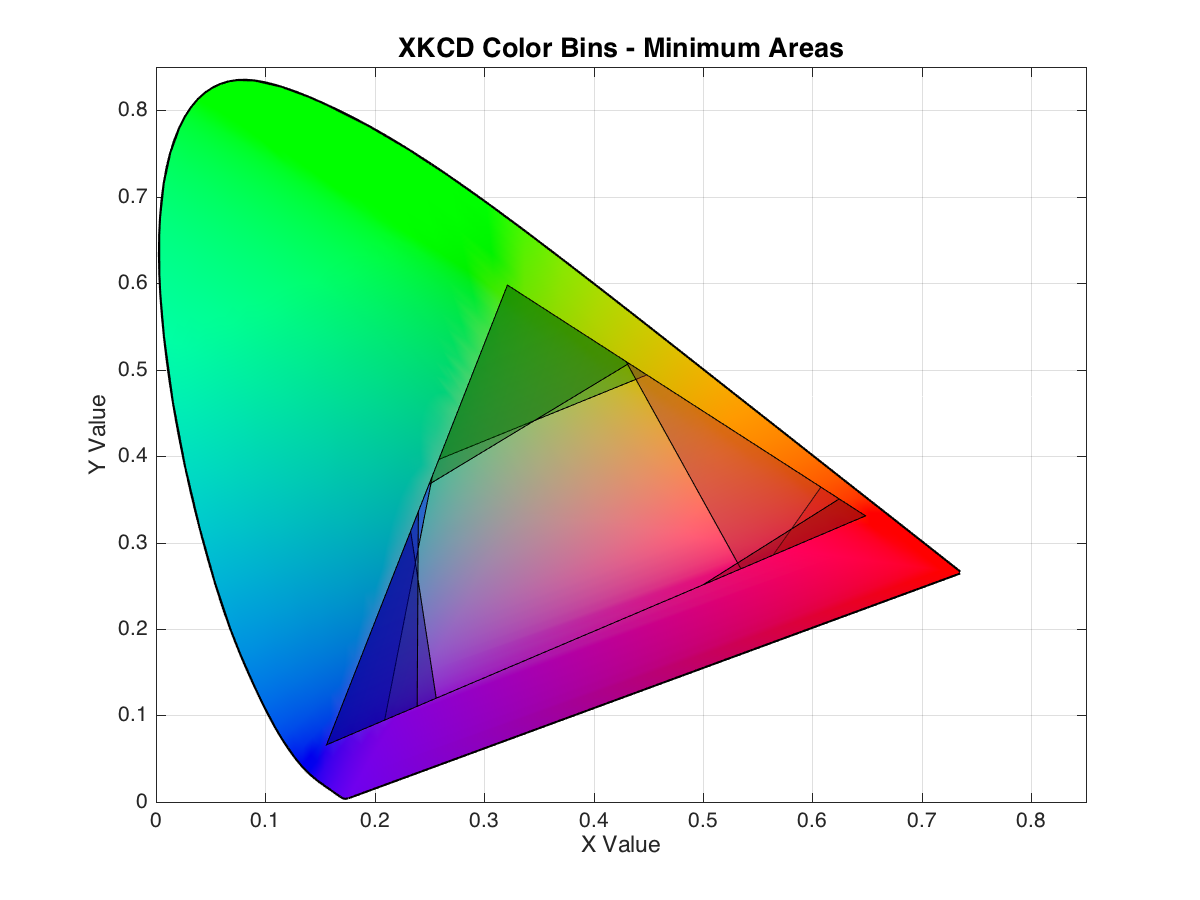
\includegraphics[width=0.9\textwidth]{images/results/colorbins_areas.png}
    \caption[XKCD Color Survey: Color Bins Minimum Areas]{XKCD Color Survey: Color Bins Minimum Areas.}
    \label{fig:colorbins_areas}
  \end{minipage}\hfill
  \begin{minipage}{0.45\textwidth}
    \centering
    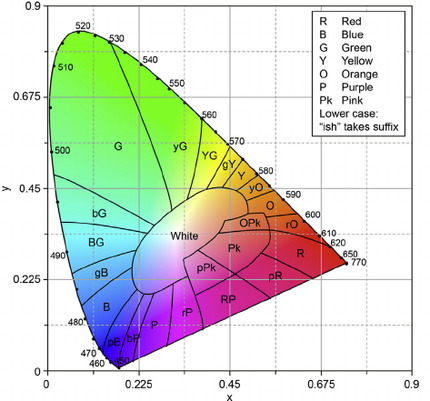
\includegraphics[width=0.87\textwidth]{images/results/cie_colors.png}
    \caption[Approximate Color Regions on CIE 1931 Chromaticity Diagram]{Approximate Color Regions on CIE 1931 Chromaticity Diagram. \cite{Fortner1997}}
    \label{fig:cie_colorregions}
  \end{minipage}
  \vspace{-15pt}
\end{figure} \par
%
However, we expected that when these color bins were drawn on a chromaticity diagram, they would create independent and more comprehensive shapes: we found that there are overlapping
values for some color bins (Figure \ref{fig:colorbins_areas}), which ultimately complicates the analysis because there is more than one possible name for the same color. For example, \emph{Blue} and \emph{Dark-Blue}
share 5 triplets: (0,0,76), (0,0,77), (0,0,78), (0,0,79) and (0,0,80); \emph{Green} and \emph{Dark-Green} share only 1 triplet, (0,57,0). This could happen since there are colors which may have ambiguous names, or
colors which are so close in the RGB cube that, for some users, it may be almost undetectable the difference between each shade. However, no repeated value was excluded from any color bin, since it would be invalid to
remove the triplet from a certain color bin: for this to be fair, we would have to randomize the process, and it would not still be fair since the the triplet is valid in both color bins. \par
%
We have solved the problem by allowing the program to find only one of the names and look no more after finding it: this is not dramatic, since the detected overlaps are from color bins which are close to each other
(the example from Green and Dark-Green, from above, is a valid one). Another way to detect the correct name is to observe the surrounding points around the value we are looking for, and attribute to that value the name
which repeats the most in its neighborhood. Currently, we are detecting the color bin which could be associated to a given value by comparing the answer with the points which form the
minimum polygon, testing if they are inside a given threshold ($threshold = 0.03$). \par
%
Moreover, the shapes created by each color bin can be depicted as \textbf{lines} if they present contiguous values in the same edge of the triangle, or as \textbf{triangles}
if the values are near the corner of the triangle and are distributed along two edges. The late situation is represented in Figure \ref{fig:colorbins_triangle}.
%
\begin{wrapfigure}[8]{r}{0.4\textwidth}
  \centering
  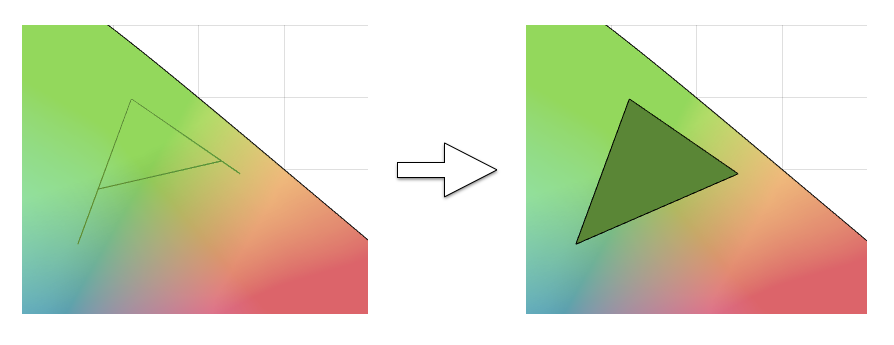
\includegraphics[width=0.4\textwidth]{images/results/colorbins_transformation.png}
  \caption[XKCD Color Survey: Color Bins Transformation]{XKCD Color Bins: Transformation from line of points, to minimum polygon.}
  \label{fig:colorbins_triangle}
\end{wrapfigure}
%
Alternatively, we could have opted for another kind of color name detection, but its implementation would be out of the scope of this Master thesis and would take a much longer
analysis than the one performed. For instance, one could have gone identifying the colors by analyzing their values and processing the wavelength originated, comparing the resulting
value with calculated areas, roughly defined by Fortner \cite{Fortner1997} and represented on Figure \ref{fig:cie_colorregions}. This idea had one problem, which was the longevity
of its solution (dated from 1997), and the inexistence of a ready-to-go implementation, completed with an \emph{svg} with all areas defined, had added weight on the decision. \par
%
Another possible method to decode colors into names would be to interpret color values and associate a color temperature, being the late one compared against a well defined table
of values; the problem here was the non-existence of table of well defined values of color temperature. Further investigation is needed to ascertain the possibility of creating such table.
%
\subsection{Outputs Generated}
\label{subsec:results_outputsgenerated}
%
Each script ends its execution when saving all the outputs referred below: it generates a set of \gls{CSV} tables ready for being analyzed by
SPSS Program, besides creating a great amount of CIE chromaticity diagrams to support the analysis. As referred before, questions 18 to 32 do not generate any output about
white answers. The outputs produced are:
%
\begin{itemize}
  \item \ul{Dataset Tables}, for laboratory, online and demographic results, as well as the one-component white answers.
  \item \ul{CIE Chromaticity Diagrams}, for laboratory, online and demographic results, as well as the one-component white answers. Particularly,
  we generate diagrams for each users group's answers, interpolated in RGB, HSV, CMYK, CIE-L*a*b* and CIE-L*C*h*.
\end{itemize}
%
%%%%%%%%%%%%%%%%%%%%%%%%%%%%%%%%%%%%%%%%%%%%%%%%%%%%%%%%%%%%%%%%%%%%%%%%%%%%%%%%%%%%%%%%%%%%%%%%%%%%%%%%%%%%%%%%%%%%%%%%%%%%%%%%%%%%%%%%%%%%%%%%%%%
%                                                                   RESULTS                                                                       %
%%%%%%%%%%%%%%%%%%%%%%%%%%%%%%%%%%%%%%%%%%%%%%%%%%%%%%%%%%%%%%%%%%%%%%%%%%%%%%%%%%%%%%%%%%%%%%%%%%%%%%%%%%%%%%%%%%%%%%%%%%%%%%%%%%%%%%%%%%%%%%%%%%%
%
\section{Results}
\label{sec:results_results}
%
In the following Section, we perform a statistical analysis of the processed data obtained from the user study. The main data to be analyzed is the one obtained in the
laboratory environment, being the online data only the corroboration of the main data. We start by drawing a profile of users who responded the survey, characterizing them as the age,
country of residence, academic degree, along with other characteristics; after, we begin drafting answers to the questions raised in the beginning of study, also referred in Section
\ref{sec:impl_objectives}, which comprises topics about \emph{Color Mixtures}, \emph{Color Models}, \emph{Color Naming} and consider differences between \emph{demographic groups}. \par
%
Note that each chromaticity diagram presented in this Section, shows a \textbf{black filled dot} which corresponds to the ideal answer for each color model, and \textbf{two black empty dots} which are the
blending-basis of questions which have asked for it; the \textbf{grey dots} represent the answers given by the users, and the black lines represent the union between each grey dot, forming each
answer pair given. \par
%
\subsection{User Profile}
\label{subsec:results_userprofile}
%
As previously said in Section \ref{sec:results_datacleaning}, we gathered a total amount of 259 users with, at least, one valid answer: from the laboratory environment
we collected 28 users, and 231 from the online strand. All of these users gave valid answers for the Profiling, Calibration and Color Deficiencies Tests Phases: the information collected
in the Profiling page is the most important to compose a user profile. \par
%
Recalling Section \ref{subsec:design_profiling}, we established that the most important information to collect were the \emph{age}, the \emph{gender}, \emph{academic degree},
\emph{nationality} and \emph{country of residence}, as well as the \emph{native language} of each user. The Table \ref{table:profiling_genderacademic} represents the frequencies of genders, ages and
academic degrees. \par
%
\begin{table}[htbp]
  \resizebox{\textwidth}{!} {
    \begin{tabular}{| l || c || c | c | c | c | c | c || c | c | c || c | c | c | c | c | c |}
      \hline
      \multicolumn{1}{|c||}{\multirow{2}{*}{Environment}} & \multirow{2}{*}{Users} & \multicolumn{6}{c||}{Ages}                                                           & \multicolumn{3}{c||}{Gender} & \multicolumn{6}{c|}{Academic Degree}                          \\ \cline{3-17}
      \multicolumn{1}{|c||}{}                             &                        & {[}0; 20{[} & {[}20; 29{]} & {[}30;39{]} & {[}40;49{]} & {[}50;59{]} & {[}60;90{]} & Female   & Male   & Other   & College & High-School & Bachelor & Master & Doctor & NoDegree \\ \hline
      Laboratory                                         & 28                     & 0           & 17           & 5           & 3           & 1           & 2            & 10       & 18     & 0        & 0       & 5           & 13       & 10     & 0      & 0        \\ \hline
      Online                                             & 231                    & 38          & 145          & 15          & 16          & 11          & 6            & 95       & 134    & 2        & 38      & 42          & 79       & 64     & 5      & 3        \\ \hline \hline
      Total                                              & 259                    & 38          & 162          & 20          & 19          & 12          & 8            & 105      & 152    & 2        & 38      & 47          & 92       & 74     & 5      & 3        \\ \hline
    \end{tabular}}
  \caption[Results: Profiling Information (Gender and Academic)]{Results: Profiling Information (Gender and Academic)}
  \vspace{-5pt}
  \label{table:profiling_genderacademic}
\end{table}
%
As seen above, our user sample is composed by 259 (100\%) users, being \textbf{105 (40.5\%) Females}, \textbf{152 (58.7\%) Males} and a minority of \textbf{2 (0.8\%) Other gendered users}: this sample age can
be characterized as being generally young ($\overline{x} = 29.77$, $\overline{x} = 23$, $s = 40.30$ ), surprisingly having \textbf{8 users (3.09\%) aged above 60 years old} which could enhance some interesting
differences between age groups. Generally, our users have hight academic qualifications, representing \textbf{66.02\% of all users (Bachelor, Master and Doctoral Degrees)}, being \textbf{38 (14.67\%) users
qualified with College degree}, \textbf{47 (18.15\%) have a High-School degree} and only \textbf{3 (1.16\%) subjects do not presented any academic degree}. Between the laboratory and online environment, the distribution
of users remains with the same proportions: more male users than females, mostly aged between 20 and 29 years old (60.71\%) and the majority having a superior academic degree (46.43\% BSc and 35.71\% MSc). \par
%
\begin{table}[htbp]
  \resizebox{\textwidth}{!} {
  \begin{tabular}{| l || c || c | c | c | c | c | c || c | c | c | c | c | c || c | c | c |}
    \hline
    \multicolumn{1}{|c||}{\multirow{2}{*}{Environment}} & \multirow{2}{*}{Users} & \multicolumn{6}{c||}{Nationality} & \multicolumn{6}{c||}{Country of Residence} & \multicolumn{3}{c|}{Languages} \\ \cline{3-17}
    \multicolumn{1}{|c||}{}                             &                        & CA  & ES & PT & UK & US & Others & CA   & DE   & GB   & PT   & US  & Others  & PT      & EN      & Others     \\ \hline
    Laboratory                                         & 28                     & 0   & 0  & 27 & 1  & 0  & 0      & 0    & 0    & 0    & 28   & 0   & 0       & 28      & 0       & 0          \\ \hline
    Online                                             & 231                    & 5   & 3  & 188& 6  & 11 & 18     & 5    & 3    & 9    & 189  & 11  & 14      & 188     & 29      & 14         \\ \hline \hline
    Total                                              & 259                    & 5   & 3  & 215& 7  & 11 & 18     & 5    & 3    & 9    & 217  & 11  & 14      & 216     & 29      & 14         \\ \hline
  \end{tabular}}
  \caption[Results: Profiling Information (Nationalities, Countries of Residence and Languages)]{Results: Profiling Information (Nationalities, Countries of Residence and Languages)}
  \vspace{-5pt}
  \label{table:profiling_nacionalities}
\end{table}
%
The Table \ref{table:profiling_nacionalities} depicts nationalities, current countries of residence and native languages spoken by our users. From the 259 (100\%) participant users,
\textbf{215 (83.01\%) of them have Portuguese nationality}, \textbf{217 (83.78\%) live in Portugal} currently and \textbf{216 (83.40\%) speak Portuguese}; the second most influent group of users are the ones from english-speaking
countries (United Kingdom, United States of America, and others). Other minor users which contributed to our survey came from Turkey, France, New Zealand, Sweden or even Antarctica (among others) -
\textbf{these countries represent only 5.41\%}. An ideal distribution of users would be such that it included enough users from all continents, which would give us room to investigate better the cultural
implications on the results; another interesting aspect would be to have users from Countries contained in the United Nations' List of Least Developed Countries\footnote{"United Nations' List of Least Developed Countries, as of May
2016", Available at: \url{un.org/en/development/desa/policy/cdp/ldc/ldc_list.pdf}. Last accessed on October 17th, 2016.} included in the sample, which was not accomplished in this study since an isolated vietnamese
user (0.39\% of the user sample) contributed to the study.
%
\subsection{Color Models}
\label{subsec:results_colormodels}
%
In this Section, we will start by analyzing the results from each question, comparing the statistics collected from each color model. Then, we are going to decompose the results by color models and evaluate which questions
had the best and worst results. Along with the statistics we are going to present, in the end we are going to map them against the questions raised before, clearly identifying them whenever they are answered. We would like
to emphasize that the important results are the ones collected in the laboratory environment: the online results will bridge and support the conclusions extracted from the laboratory conditions. The values presented as "distances"
are measured inside the finite interval $[0 ; 1]$, since the CIE Chromaticity Diagram has its values comprised between this interval. \par
%
\begin{table}[!htbp]
  \centering
  \resizebox{0.8\textwidth}{!} {
  \begin{tabular}{@{}cccccccccccccc@{}}
                                  &                                                       & \multicolumn{2}{c}{Reference Pairs}                         & \multicolumn{5}{c}{Laboratory Environment}                                                                                                                                                                                                                                      & \multicolumn{5}{c}{Online Environment}                                                                                                                                                                                                                                                                         \\ \cmidrule(l){3-14}
    \multirow{-2}{*}{Question ID} & \multirow{-2}{*}{Presented Color}                     & C1                           & \multicolumn{1}{c|}{C2}      & HSV                                                         & CIE-L*C*h*                                                 & CMYK                                                       & RGB                        & \multicolumn{1}{c||}{CIE-L*a*b*}                            & HSV                                                        & CIE-L*C*h*                                                 & CMYK                                                       & RGB                                                        & \multicolumn{1}{c|}{CIE-L*a*b*}                            \\ \midrule
    \multicolumn{1}{c}{1}       & \multicolumn{1}{c}{\cellcolor[HTML]{FFFF00}\#FFFF00} & \multicolumn{1}{c|}{Red}     & \multicolumn{1}{c|}{Green}   & \multicolumn{1}{c|}{0.13}                                   & \multicolumn{1}{c|}{0.2}                                   & \multicolumn{1}{c|}{\cellcolor[HTML]{32CB00}\textbf{0.09}} & \multicolumn{1}{c|}{0.12}  & \multicolumn{1}{c||}{0.12}                                  & \multicolumn{1}{c|}{0.07}                                  & \multicolumn{1}{c|}{0.21}                                  & \multicolumn{1}{c|}{\cellcolor[HTML]{32CB00}\textbf{0.06}} & \multicolumn{1}{c|}{0.07}                                  & \multicolumn{1}{c|}{0.07}                                  \\ \midrule
    \multicolumn{1}{c}{2}       & \multicolumn{1}{c}{\cellcolor[HTML]{FF00FF}\#FF00FF} & \multicolumn{1}{c|}{Red}     & \multicolumn{1}{c|}{Blue}    & \multicolumn{1}{c|}{0.22}                                   & \multicolumn{1}{c|}{0.16}                                  & \multicolumn{1}{c|}{\cellcolor[HTML]{32CB00}\textbf{0.11}} & \multicolumn{1}{c|}{0.17}  & \multicolumn{1}{c||}{0.16}                                  & \multicolumn{1}{c|}{0.15}                                  & \multicolumn{1}{c|}{0.16}                                  & \multicolumn{1}{c|}{\cellcolor[HTML]{32CB00}\textbf{0.08}} & \multicolumn{1}{c|}{0.1}                                   & \multicolumn{1}{c|}{0.12}                                  \\ \midrule
    \multicolumn{1}{c}{3}       & \multicolumn{1}{c}{\cellcolor[HTML]{80FF00}\#80FF00} & \multicolumn{1}{c|}{Red}     & \multicolumn{1}{c|}{Cyan}    & \multicolumn{1}{c|}{\cellcolor[HTML]{32CB00}\textbf{0.045}} & \multicolumn{1}{c|}{0.215}                                 & \multicolumn{1}{c|}{0.05}                                  & \multicolumn{1}{c|}{0.095} & \multicolumn{1}{c||}{0.11}                                  & \multicolumn{1}{c|}{\cellcolor[HTML]{32CB00}\textbf{0.04}} & \multicolumn{1}{c|}{0.21}                                  & \multicolumn{1}{c|}{0.06}                                  & \multicolumn{1}{c|}{0.11}                                  & \multicolumn{1}{c|}{0.11}                                  \\ \midrule
    \multicolumn{1}{c}{4}       & \multicolumn{1}{c}{\cellcolor[HTML]{7F00FF}\#7F00FF} & \multicolumn{1}{c|}{Red}     & \multicolumn{1}{c|}{Cyan}    & \multicolumn{1}{c|}{0.12}                                   & \multicolumn{4}{c||}{}                                                                                                                                                                                             & \multicolumn{1}{c|}{0.11}                                  & \multicolumn{4}{c|}{}                                                                                                                                                                                                                             \\ \midrule
    \multicolumn{1}{c}{5}       & \multicolumn{1}{c}{\cellcolor[HTML]{FF0080}\#FF0080} & \multicolumn{1}{c|}{Red}     & \multicolumn{1}{c|}{Magenta} & \multicolumn{1}{c|}{0.17}                                   & \multicolumn{1}{c|}{0.15}                                  & \multicolumn{1}{c|}{\cellcolor[HTML]{32CB00}\textbf{0.13}} & \multicolumn{1}{c|}{0.14}  & \multicolumn{1}{c||}{0.14}                                  & \multicolumn{1}{c|}{0.16}                                  & \multicolumn{1}{c|}{0.15}                                  & \multicolumn{1}{c|}{\cellcolor[HTML]{32CB00}\textbf{0.13}} & \multicolumn{1}{c|}{0.14}                                  & \multicolumn{1}{c|}{0.11}                                  \\ \midrule
    \multicolumn{1}{c}{6}       & \multicolumn{1}{c}{\cellcolor[HTML]{FF8000}\#FF8000} & \multicolumn{1}{c|}{Red}     & \multicolumn{1}{c|}{Yellow}  & \multicolumn{1}{c|}{0.07}                                   & \multicolumn{1}{c|}{0.13}                                  & \multicolumn{1}{c|}{0.06}                                  & \multicolumn{1}{c|}{0.08}  & \multicolumn{1}{c||}{\cellcolor[HTML]{32CB00}\textbf{0.05}} & \multicolumn{1}{c|}{0.03}                                  & \multicolumn{1}{c|}{0.14}                                  & \multicolumn{1}{c|}{0.03}                                  & \multicolumn{1}{c|}{0.04}                                  & \multicolumn{1}{c|}{\cellcolor[HTML]{32CB00}\textbf{0.02}} \\ \midrule
    \multicolumn{1}{c}{7}       & \multicolumn{1}{c}{\cellcolor[HTML]{0000FF}\#0000FF} & \multicolumn{1}{c|}{Cyan}    & \multicolumn{1}{c|}{Magenta} & \multicolumn{1}{c|}{0.16}                                   & \multicolumn{1}{c|}{0.23}                                  & \multicolumn{1}{c|}{\cellcolor[HTML]{32CB00}\textbf{0.10}} & \multicolumn{1}{c|}{0.15}  & \multicolumn{1}{c||}{0.17}                                  & \multicolumn{1}{c|}{0.13}                                  & \multicolumn{1}{c|}{0.18}                                  & \multicolumn{1}{c|}{\cellcolor[HTML]{32CB00}\textbf{0.11}} & \multicolumn{1}{c|}{0.17}                                  & \multicolumn{1}{c|}{0.22}                                  \\ \midrule
    \multicolumn{1}{c}{8}       & \multicolumn{1}{c}{\cellcolor[HTML]{FF0000}\#FF0000} & \multicolumn{1}{c|}{Magenta} & \multicolumn{1}{c|}{Yellow}  & \multicolumn{1}{c|}{\cellcolor[HTML]{32CB00}\textbf{0.10}}  & \multicolumn{1}{c|}{0.17}                                  & \multicolumn{1}{c|}{\cellcolor[HTML]{32CB00}\textbf{0.10}} & \multicolumn{1}{c|}{0.13}  & \multicolumn{1}{c||}{0.13}                                  & \multicolumn{1}{c|}{0.10}                                  & \multicolumn{1}{c|}{\cellcolor[HTML]{32CB00}\textbf{0.09}} & \multicolumn{1}{c|}{0.12}                                  & \multicolumn{1}{c|}{0.14}                                  & \multicolumn{1}{c|}{0.16}                                  \\ \midrule
    \multicolumn{1}{c}{9}       & \multicolumn{1}{c}{\cellcolor[HTML]{00FF80}\#00FF80} & \multicolumn{1}{c|}{Green}   & \multicolumn{1}{c|}{Cyan}    & \multicolumn{1}{c|}{0.13}                                   & \multicolumn{1}{c|}{0.16}                                  & \multicolumn{1}{c|}{\cellcolor[HTML]{32CB00}\textbf{0.09}} & \multicolumn{1}{c|}{0.10}  & \multicolumn{1}{c||}{0.11}                                  & \multicolumn{1}{c|}{0.11}                                  & \multicolumn{1}{c|}{0.13}                                  & \multicolumn{1}{c|}{\cellcolor[HTML]{32CB00}\textbf{0.10}} & \multicolumn{1}{c|}{\cellcolor[HTML]{32CB00}\textbf{0.10}} & \multicolumn{1}{c|}{0.11}                                  \\ \midrule
    \multicolumn{1}{c}{10}      & \multicolumn{1}{c}{\cellcolor[HTML]{0080FF}\#0080FF} & \multicolumn{1}{c|}{Green}   & \multicolumn{1}{c|}{Magenta} & \multicolumn{1}{c|}{0.30}                                   & \multicolumn{1}{c|}{0.26}                                  & \multicolumn{1}{c|}{\cellcolor[HTML]{32CB00}\textbf{0.13}} & \multicolumn{1}{c|}{0.21}  & \multicolumn{1}{c||}{0.20}                                  & \multicolumn{1}{c|}{0.17}                                  & \multicolumn{1}{c|}{0.27}                                  & \multicolumn{1}{c|}{\cellcolor[HTML]{32CB00}\textbf{0.13}} & \multicolumn{1}{c|}{0.20}                                  & \multicolumn{1}{c|}{0.22}                                  \\ \midrule
    \multicolumn{1}{c}{11}      & \multicolumn{1}{c}{\cellcolor[HTML]{FF8000}\#FF8000} & \multicolumn{1}{c|}{Green}   & \multicolumn{1}{c|}{Magenta} & \multicolumn{1}{c|}{\cellcolor[HTML]{32CB00}\textbf{0.06}}  & \multicolumn{4}{c||}{}                                                                                                                                                                                             & \multicolumn{1}{c|}{\cellcolor[HTML]{32CB00}\textbf{0.04}} & \multicolumn{4}{c|}{}                                                                                                                                                                                                                             \\ \midrule
    \multicolumn{1}{c}{12}      & \multicolumn{1}{c}{\cellcolor[HTML]{80FF00}\#80FF00} & \multicolumn{1}{c|}{Green}   & \multicolumn{1}{c|}{Yellow}  & \multicolumn{1}{c|}{\cellcolor[HTML]{32CB00}\textbf{0.11}}  & \multicolumn{1}{c|}{0.23}                                  & \multicolumn{1}{c|}{0.13}                                  & \multicolumn{1}{c|}{0.15}  & \multicolumn{1}{c||}{0.17}                                  & \multicolumn{1}{c|}{\cellcolor[HTML]{32CB00}\textbf{0.08}} & \multicolumn{1}{c|}{0.24}                                  & \multicolumn{1}{c|}{0.12}                                  & \multicolumn{1}{c|}{0.13}                                  & \multicolumn{1}{c|}{0.15}                                  \\ \midrule
    \multicolumn{1}{c}{13}      & \multicolumn{1}{c}{\cellcolor[HTML]{0080FF}\#0080FF} & \multicolumn{1}{c|}{Blue}    & \multicolumn{1}{c|}{Cyan}    & \multicolumn{1}{c|}{0.27}                                   & \multicolumn{1}{c|}{\cellcolor[HTML]{32CB00}\textbf{0.17}} & \multicolumn{1}{c|}{0.19}                                  & \multicolumn{1}{c|}{0.25}  & \multicolumn{1}{c||}{0.23}                                  & \multicolumn{1}{c|}{0.14}                                  & \multicolumn{1}{c|}{0.20}                                  & \multicolumn{1}{c|}{0.14}                                  & \multicolumn{1}{c|}{\cellcolor[HTML]{32CB00}\textbf{0.13}} & \multicolumn{1}{c|}{0.14}                                  \\ \midrule
    \multicolumn{1}{c}{14}      & \multicolumn{1}{c}{\cellcolor[HTML]{8000FF}\#8000FF} & \multicolumn{1}{c|}{Blue}    & \multicolumn{1}{c|}{Magenta} & \multicolumn{1}{c|}{0.12}                                   & \multicolumn{1}{c|}{0.30}                                  & \multicolumn{1}{c|}{\cellcolor[HTML]{32CB00}\textbf{0.10}} & \multicolumn{1}{c|}{0.13}  & \multicolumn{1}{c||}{0.13}                                  & \multicolumn{1}{c|}{0.10}                                  & \multicolumn{1}{c|}{0.29}                                  & \multicolumn{1}{c|}{\cellcolor[HTML]{32CB00}\textbf{0.09}} & \multicolumn{1}{c|}{0.11}                                  & \multicolumn{1}{c|}{0.12}                                  \\ \midrule
    \multicolumn{1}{c}{15}      & \multicolumn{1}{c}{\cellcolor[HTML]{00FF80}\#00FF80} & \multicolumn{1}{c|}{Blue}    & \multicolumn{1}{c|}{Yellow}  & \multicolumn{1}{c|}{0.09}                                   & \multicolumn{1}{c|}{0.30}                                  & \multicolumn{1}{c|}{\cellcolor[HTML]{32CB00}\textbf{0.06}} & \multicolumn{1}{c|}{0.11}  & \multicolumn{1}{c||}{0.13}                                  & \multicolumn{1}{c|}{0.11}                                  & \multicolumn{1}{c|}{0.30}                                  & \multicolumn{1}{c|}{\cellcolor[HTML]{32CB00}\textbf{0.06}} & \multicolumn{1}{c|}{0.11}                                  & \multicolumn{1}{c|}{0.13}                                  \\ \midrule
    \multicolumn{1}{c}{16}      & \multicolumn{1}{c}{\cellcolor[HTML]{FF007F}\#FF007F} & \multicolumn{1}{c|}{Blue}    & \multicolumn{1}{c|}{Yellow}  & \multicolumn{1}{c|}{0.21}                                   & \multicolumn{4}{c||}{}                                                                                                                                                                                             & \multicolumn{1}{c|}{0.19}                                  & \multicolumn{4}{c|}{}                                                                                                                                                                                                                             \\ \midrule
    \multicolumn{1}{c}{17}      & \multicolumn{1}{c}{\cellcolor[HTML]{00FF00}\#00FF00} & \multicolumn{1}{c|}{Cyan}    & \multicolumn{1}{c|}{Yellow}  & \multicolumn{1}{c|}{0.07}                                   & \multicolumn{1}{c|}{0.16}                                  & \multicolumn{1}{c|}{\cellcolor[HTML]{32CB00}\textbf{0.05}} & \multicolumn{1}{c|}{0.10}  & \multicolumn{1}{c||}{0.11}                                  & \multicolumn{1}{c|}{0.08}                                  & \multicolumn{1}{c|}{0.17}                                  & \multicolumn{1}{c|}{\cellcolor[HTML]{32CB00}\textbf{0.05}} & \multicolumn{1}{c|}{0.10}                                  & \multicolumn{1}{c|}{0.11}                                  \\ \bottomrule
  \end{tabular}}
  \caption[Distances of Results Interpolated in each Color Model]{Distances between interpolated results in each Color Model, to the ideal pre-calculated answer.}
  \vspace{-5pt}
  \label{table:colormodels_distances_labonline}
\end{table}
%
As referred before, each answer pair given from our users on questions 1 to 17 (one color given, two colors asked) was interpolated in five color models:
HSV, CIE-L*C*h*, CMYK, RGB and CIE-L*a*b*. Then, we have converted the result into CIE-XYZ values, so the comparison between the pre-calculated blend for
each color model and the given answer-pair would be conveyed in a standard color model. However, since the CIE-XYZ color model represents a 3D color space
and we are representing our values in the same plane of maximum saturation, the XYZ coordinates had to be flattened down to XY coordinates only, dropping
the Z component: this is a conversion from CIE-XYZ to CIE-XYY, where the X and Y coordinates were divided by the sum of all XYZ coordinates. Then, the
euclidean distance between this interpolated blend and the one pre-calculated was measured, indicating us the proximity of the user's answers to each
color model. \textbf{It was this distance which we had considered when analyzing the relationship between the users' expectations and each color model}.
In order to improve this analysis, we present Table \ref{table:colormodels_distances_labonline} which contains the mean value for these distances,
according to each color model for each question, in each study environment. Colored in green are, the color model which has the
smallest distance, \emph{per} question, in each environment. \par
%
%%%%%%%%%%%%%%%%%%%%%%%%%%%%%%%%%%%%%%%%%%%%%%%%%%%%%%%%%%%%%%%%%%%%%%%%%%%%%%%%%
%
\subsubsection{Analyzing Questions}
\label{subsubsec:questions_analyzing}
%
The importance of breaking down the evaluation into questions is such that, it is relevant to understand, at least, which color models have the best
results for each mixture. The results from this Section will be critical to determine later which color models are more compatible with each mixture,
which model yields better results and others who do not. In order to present the colors to the user, in the interface, we interpolated the colors from
each color blending according to the HSV model, since it provides three parameters which are convenient for us to manipulate (the hue, saturation and value).
Therefore, \textbf{the resulting colors which we present to the user when asking him the blending-basis are blended in HSV} for convenience. However, as
said before, we intended to compare the interpolated answer pairs given by the users, to each of the previously referred color models: as it will be seen
on each question below, we compared these answers with the pre-calculated values for each blending in each color model. For example, the answers were
interpolated in CIE-L*C*h*, and then they were compared with the result which was supposed to happen when blending the two colors from that question, in
CIE-L*C*h*. \par
%
On the other hand, when the blending-basis was given to the user and we intended to test which resulting color the users would tend to, we needed to give
them every pre-calculated result, in every color model: this way, \textbf{we presented to the user the entire set of pre-calculated blending results,
containing the results from HSV, CIE-L*C*h*, CMYK, RGB and CIE-L*a*b*}. \par
%
The triples presented in tables below represent the resulting color of each color blending, \emph{per} color model, and it is
a XYZ Triple value that maps that color on the CIE Chromaticity Diagram.
%
\paragraph{\ul{Question One}}
%
One can observe that the model which presents the lowest mean value is the CMYK ($\overline{x} = 0.09$), possibly indicating that this model yields
the best results for this question, while HSV, RGB and CIE-L*a*b* have closer values. A Friedman Test showed that there are, indeed, significant
differences ($\chi^2 = 48.568$, $p < 0.05$) between each color model.
Further analysis with the Wilcoxon Test reveals that CMYK ($p < 0.05$) has, in fact, very different responses from the other color models, which leads
us to conclude that \textbf{the CMYK Color Model is the best model to represent yellow blends}. Since HSV, RGB and CIE-L*a*b* have similar mean values,
we tried to compare them between each other: \textbf{there is no statistically significant differences among HSV, RGB and CIE-L*a*b*, whereby there is insufficient
information to evaluate this color models regarding this color mixture}. According to table, it is also possible to say that \textbf{CMYK Color Model
presents a low deviation}, not only in laboratory results ($s_{lab} = 0.06$). \par
%
It is safe to say that \textbf{CIE-L*C*h* has the worst performance against the other color models}, since its mean is the highest of all
($\overline{x} = 0.20$), and the values from Wilcoxon Test ($p < 0.05$) indicates that this color model has statistically significant differences every
other model. \textbf{These results are corroborated by the online users}, since a Wilcoxon Test shows that there are no statistically significant
differences between the laboratory distances and online ones ($p < 0.05$).
%
\begin{table}[H]
  \resizebox{\textwidth}{!} {
  \begin{tabular}{lccccccccccccc}
    \hline
    \multicolumn{1}{c}{}                              &                                      & \multicolumn{2}{c}{Reference Pair}                   & \multicolumn{10}{c}{Possible Results}                                                                                                                                                                                                                                                                                        \\ \cline{3-14}
    \multicolumn{1}{c}{\multirow{-2}{*}{Question ID}} & \multirow{-2}{*}{Given Color}        & C1                       & C2                         & \multicolumn{2}{c}{HSV}                                        & \multicolumn{2}{c}{CIE-L*C*h*}                                 & \multicolumn{2}{c}{CMYK}                                       & \multicolumn{2}{c}{RGB}                                        & \multicolumn{2}{c}{CIE-L*a*b*}                                 \\ \hline
    \multicolumn{1}{c}{1}                             & \cellcolor[HTML]{FFFF00}(77, 93, 14) & \multicolumn{1}{c|}{Red} & \multicolumn{1}{c|}{Green} & \multicolumn{2}{c|}{\cellcolor[HTML]{FFFF00}(77, 93, 14)}      & \multicolumn{2}{c|}{\cellcolor[HTML]{D7A700}(42, 42, 6)}       & \multicolumn{2}{c|}{\cellcolor[HTML]{808000}(17, 20, 3)}       & \multicolumn{2}{c|}{\cellcolor[HTML]{808000}(17, 20, 3)}       & \multicolumn{2}{c|}{\cellcolor[HTML]{C9AB00}(39, 42, 6)}       \\ \hline
                                                      & \multicolumn{1}{l}{}                 & \multicolumn{1}{l}{}     & \multicolumn{1}{l}{}       & \multicolumn{1}{c}{$\overline{x}$} & \multicolumn{1}{c}{$s$} & \multicolumn{1}{c}{$\overline{x}$} & \multicolumn{1}{c}{$s$} & \multicolumn{1}{c}{$\overline{x}$} & \multicolumn{1}{c}{$s$} & \multicolumn{1}{c}{$\overline{x}$} & \multicolumn{1}{c}{$s$} & \multicolumn{1}{c}{$\overline{x}$} & \multicolumn{1}{c}{$s$} \\ \hline
    \multicolumn{4}{l}{Distance to Objective - Laboratory}                                                                                           & \multicolumn{1}{|c}{0.13}       & \multicolumn{1}{c|}{0.08}    & \multicolumn{1}{|c}{0.2}        & \multicolumn{1}{c|}{0.06}    & \multicolumn{1}{|c}{\textbf{0.09}}       & \multicolumn{1}{c|}{0.06}    & \multicolumn{1}{|c}{0.12}       & \multicolumn{1}{c|}{0.08}    & \multicolumn{1}{|c}{0.12}       & \multicolumn{1}{c|}{0.08}    \\
    \multicolumn{4}{l}{Distance to Objective - Online}                                                                                               & \multicolumn{1}{|c}{0.07}       & \multicolumn{1}{c|}{0.09}    & \multicolumn{1}{|c}{0.21}       & \multicolumn{1}{c|}{0.07}    & \multicolumn{1}{|c}{\textbf{0.06}}       & \multicolumn{1}{c|}{0.06}    & \multicolumn{1}{|c}{0.07}       & \multicolumn{1}{c|}{0.09}    & \multicolumn{1}{|c}{0.07}       & \multicolumn{1}{c|}{0.08}    \\ \hline
    \end{tabular}}
  \caption[Question 1, with expected Results.]{Question 1: expected colors, possible results and statistics of distances to Objective.}
  \vspace{-5pt}
  \label{table:lab_q1_expected}
\end{table}
%
\paragraph{\ul{Question Two}}
%
CMYK Color Model presents, yet again, the lowest mean value for distance to ideal answer ($\overline{x} = 0.11$).
However, it is not safe to say that which color model had the worst results: judging by laboratory values, the HSV Color Model would not only
the have highest mean distance, but also the largest deviation of answers; yet, evaluating the online results, it would CIE-L*C*h* to occupy
such position. Performing a Friedman Test, we can conclude that there are, in fact, significant differences ($\chi^2 = 22.041$, $p < 0.05$) between
the color models; post hoc Wilcoxon Analysis ($p < 0.05$) reveals CMYK has statistically different results from every other color model, therefore
concluding that \textbf{CMYK has the best solution for this blending}.\par
%
The tendency of results to blend Magenta in CMYK Color Model, could be explained by the fact that magenta is a primitive color of such model,
therefore leading the user to blend it accordingly. In this question, \textbf{CIE-L*C*h* has only significant differences with HSV ($p < 0.05$)},
which is far opposite from question 1. The online results for this question validate the laboratory experience, since a Wilcoxon Test show that there
are no statistically significant differences between the laboratory distances and online ones ($p < 0.05$).
%
\begin{table}[H]
  \resizebox{\textwidth}{!} {
  \begin{tabular}{lccccccccccccc}
    \hline
    \multicolumn{1}{c}{}                              &                                      & \multicolumn{2}{c}{Reference Pair}                   & \multicolumn{10}{c}{Possible Results}                                                                                                                                                                                                                                                                                        \\ \cline{3-14}
    \multicolumn{1}{c}{\multirow{-2}{*}{Question ID}} & \multirow{-2}{*}{Given Color}        & C1                       & C2                         & \multicolumn{2}{c}{HSV}                                        & \multicolumn{2}{c}{CIE-L*C*h*}                                 & \multicolumn{2}{c}{CMYK}                                       & \multicolumn{2}{c}{RGB}                                        & \multicolumn{2}{c}{CIE-L*a*b*}                                 \\ \hline
    \multicolumn{1}{c}{2}                             & \cellcolor[HTML]{FF00FF}(59, 28, 97) & \multicolumn{1}{c|}{Red} & \multicolumn{1}{c|}{Blue}  & \multicolumn{2}{c|}{\cellcolor[HTML]{FF00FF}(59, 28, 97)}      & \multicolumn{2}{c|}{\cellcolor[HTML]{FB0080}{\color[HTML]{FFFFFF}(44, 22, 22)}}       & \multicolumn{2}{c|}{\cellcolor[HTML]{800080}{\color[HTML]{FFFFFF}(13, 6, 21)}}       & \multicolumn{2}{c|}{\cellcolor[HTML]{800080}{\color[HTML]{FFFFFF}(13, 6, 21)}}       & \multicolumn{2}{c|}{\cellcolor[HTML]{CA0088}(29, 14, 25)}       \\ \hline
                                                      & \multicolumn{1}{l}{}                 & \multicolumn{1}{l}{}     & \multicolumn{1}{l}{}       & \multicolumn{1}{c}{$\overline{x}$} & \multicolumn{1}{c}{$s$} & \multicolumn{1}{c}{$\overline{x}$} & \multicolumn{1}{c}{$s$} & \multicolumn{1}{c}{$\overline{x}$} & \multicolumn{1}{c}{$s$} & \multicolumn{1}{c}{$\overline{x}$} & \multicolumn{1}{c}{$s$} & \multicolumn{1}{c}{$\overline{x}$} & \multicolumn{1}{c}{$s$} \\ \hline
    \multicolumn{4}{l}{Distance to Objective - Laboratory}                                                                                           & \multicolumn{1}{|c}{0.22}       & \multicolumn{1}{c|}{0.13}    & \multicolumn{1}{|c}{0.16}       & \multicolumn{1}{c|}{0.09}    & \multicolumn{1}{|c}{\textbf{0.11}}       & \multicolumn{1}{c|}{0.06}    & \multicolumn{1}{|c}{0.17}       & \multicolumn{1}{c|}{0.11}    & \multicolumn{1}{|c}{0.16}       & \multicolumn{1}{c|}{0.08}    \\
    \multicolumn{4}{l}{Distance to Objective - Online}                                                                                               & \multicolumn{1}{|c}{0.15}       & \multicolumn{1}{c|}{0.13}    & \multicolumn{1}{|c}{0.16}       & \multicolumn{1}{c|}{0.08}    & \multicolumn{1}{|c}{\textbf{0.08}}       & \multicolumn{1}{c|}{0.04}    & \multicolumn{1}{|c}{0.1}        & \multicolumn{1}{c|}{0.08}    & \multicolumn{1}{|c}{0.12}       & \multicolumn{1}{c|}{0.05}    \\ \hline
    \end{tabular}}
  \caption[Question 2, with expected Results.]{Question 2: expected colors, possible results and statistics of distances to Objective.}
  \vspace{-5pt}
  \label{table:lab_q2_expected}
\end{table}
%
\paragraph{\ul{Question Three}}
%
It is observable that CMYK Color Model presents the lowest mean value for distance to ideal answer ($\overline{x} = 0.05$); however,
the standard deviation for the HSV Color Model is the highest between both study environments ($s = 0.12$).
Running the Friedman Test, we can conclude that there are significant differences ($\chi^2 = 84.448$, $p < 0.05$) between the color models;
Wilcoxon Analysis ($p < 0.05$) reveals that CMYK has statistically different results from other color models (except RGB), therefore concluding that
\textbf{CMYK has the best solution for this blending}. CIE-L*C*h* is again the lower color model being
significantly different from every other color model. \par
%
Once again, these results are validated by the online users' dataset, since a Wilcoxon Test show that there are no statistically significant differences between the laboratory
distances and online ones ($p < 0.05$).The results from this question will be useful later, when analyzing question twelve.
%
\begin{table}[H]
  \resizebox{\textwidth}{!} {
  \begin{tabular}{lccccccccccccc}
    \hline
    \multicolumn{1}{c}{}                              &                                      & \multicolumn{2}{c}{Reference Pair}                   & \multicolumn{10}{c}{Possible Results}                                                                                                                                                                                                                                                                                        \\ \cline{3-14}
    \multicolumn{1}{c}{\multirow{-2}{*}{Question ID}} & \multirow{-2}{*}{Given Color}        & C1                       & C2                         & \multicolumn{2}{c}{HSV}                                        & \multicolumn{2}{c}{CIE-L*C*h*}                                 & \multicolumn{2}{c}{CMYK}                                       & \multicolumn{2}{c}{RGB}                                        & \multicolumn{2}{c}{CIE-L*a*b*}                                 \\ \hline
    \multicolumn{1}{c}{3}                             & \cellcolor[HTML]{80FF00}(45, 76, 12) & \multicolumn{1}{c|}{Red} & \multicolumn{1}{c|}{Cyan}  & \multicolumn{2}{c|}{\cellcolor[HTML]{80FF00}(45, 76, 12)}      & \multicolumn{2}{c|}{\cellcolor[HTML]{91C01D}(31, 44, 8)}       & \multicolumn{2}{c|}{\cellcolor[HTML]{808080}{\color[HTML]{FFFFFF}(21, 22, 24)}}       & \multicolumn{2}{c|}{\cellcolor[HTML]{808080}{\color[HTML]{FFFFFF}(21, 22, 24)}}       & \multicolumn{2}{c|}{\cellcolor[HTML]{DDA581}(47, 44, 27)}       \\ \hline
                                                      & \multicolumn{1}{l}{}                 & \multicolumn{1}{l}{}     & \multicolumn{1}{l}{}       & \multicolumn{1}{c}{$\overline{x}$} & \multicolumn{1}{c}{$s$} & \multicolumn{1}{c}{$\overline{x}$} & \multicolumn{1}{c}{$s$} & \multicolumn{1}{c}{$\overline{x}$} & \multicolumn{1}{c}{$s$} & \multicolumn{1}{c}{$\overline{x}$} & \multicolumn{1}{c}{$s$} & \multicolumn{1}{c}{$\overline{x}$} & \multicolumn{1}{c}{$s$} \\ \hline
    \multicolumn{4}{l}{Distance to Objective - Laboratory}                                                                                           & \multicolumn{1}{|c}{0.094}       & \multicolumn{1}{c|}{0.12}    & \multicolumn{1}{|c}{0.23}       & \multicolumn{1}{c|}{0.06}    & \multicolumn{1}{|c}{\textbf{0.061}}       & \multicolumn{1}{c|}{0.03}    & \multicolumn{1}{|c}{0.11}       & \multicolumn{1}{c|}{0.06}    & \multicolumn{1}{|c}{0.12}       & \multicolumn{1}{c|}{0.04}    \\
    \multicolumn{4}{l}{Distance to Objective - Online}                                                                                               & \multicolumn{1}{|c}{\textbf{0.07}}        & \multicolumn{1}{c|}{0.09}    & \multicolumn{1}{|c}{0.23}        & \multicolumn{1}{c|}{0.06}    & \multicolumn{1}{|c}{\textbf{0.07}}       & \multicolumn{1}{c|}{0.03}    & \multicolumn{1}{|c}{0.12}        & \multicolumn{1}{c|}{0.06}    & \multicolumn{1}{|c}{0.13}       & \multicolumn{1}{c|}{0.04}    \\ \hline
    \end{tabular}}
  \caption[Question 3, with expected Results.]{Question 3: expected colors, possible results and statistics of distances to Objective.}
  \vspace{-5pt}
  \label{table:lab_q3_expected}
\end{table}
%
\paragraph{\ul{Question Four}}
%
This one is the second possible output from the blend of \ul{Red and Cyan colors}. Comparing the results for the HSV Color Model of both questions, mean distances are quite lower for question thirteen
($\overline{x} = 0.045$), whilst the deviation of answers is higher in both questions. \par
%
Based on these results, we can conclude \textbf{users tend to blend in CMYK Color Model to obtain a green color}, \textbf{mixing red and cyan
does not generate a purple shade, according to users' expectations}. \textbf{These results are corroborated by the online users}, since a Wilcoxon
Test show that there are no statistically significant differences between the laboratory distances and online ones ($p < 0.05$).
%
\begin{table}[H]
  \resizebox{\textwidth}{!} {
  \begin{tabular}{lccccccccccccc}
    \hline
    \multicolumn{1}{c}{}                              &                                      & \multicolumn{2}{c}{Reference Pair}                   & \multicolumn{10}{c}{Possible Results}                                                                                                                                                                                                                                                                                        \\ \cline{3-14}
    \multicolumn{1}{c}{\multirow{-2}{*}{Question ID}} & \multirow{-2}{*}{Given Color}        & C1                       & C2                         & \multicolumn{2}{c}{HSV}                                        & \multicolumn{2}{c}{CIE-L*C*h*}                                 & \multicolumn{2}{c}{CMYK}                                       & \multicolumn{2}{c}{RGB}                                        & \multicolumn{2}{c}{CIE-L*a*b*}                                 \\ \hline
    \multicolumn{1}{c}{4}                             & \cellcolor[HTML]{7F00FF}{\color[HTML]{FFFFFF}(27, 12, 95)} & \multicolumn{1}{c|}{Red} & \multicolumn{1}{c|}{Cyan}  & \multicolumn{2}{c|}{\cellcolor[HTML]{FF00FF}(59, 28, 97)}      & \multicolumn{2}{c|}{\cellcolor[HTML]{91C01D}(31, 44, 8)}       & \multicolumn{2}{c|}{\cellcolor[HTML]{808080}{\color[HTML]{FFFFFF}(21, 22, 24)}}       & \multicolumn{2}{c|}{\cellcolor[HTML]{808080}{\color[HTML]{FFFFFF}(21, 22, 24)}}       & \multicolumn{2}{c|}{\cellcolor[HTML]{DDA581}(47, 44, 27)}       \\ \hline
                                                      & \multicolumn{1}{l}{}                 & \multicolumn{1}{l}{}     & \multicolumn{1}{l}{}       & \multicolumn{1}{c}{$\overline{x}$} & \multicolumn{1}{c}{$s$} & \multicolumn{1}{c}{$\overline{x}$} & \multicolumn{1}{c}{$s$} & \multicolumn{1}{c}{$\overline{x}$} & \multicolumn{1}{c}{$s$} & \multicolumn{1}{c}{$\overline{x}$} & \multicolumn{1}{c}{$s$} & \multicolumn{1}{c}{$\overline{x}$} & \multicolumn{1}{c}{$s$} \\ \hline
    \multicolumn{4}{l}{Distance to Objective - Laboratory}                                                                                           & \multicolumn{1}{|c}{0.12}       & \multicolumn{1}{c|}{0.13}    & \multicolumn{1}{|c}{0.20}       & \multicolumn{1}{c|}{0.06}    & \multicolumn{1}{|c}{\textbf{0.10}}         & \multicolumn{1}{c|}{0.04}    & \multicolumn{1}{|c}{0.19}       & \multicolumn{1}{c|}{0.06}    & \multicolumn{1}{|c}{0.20}       & \multicolumn{1}{c|}{0.09}    \\
    \multicolumn{4}{l}{Distance to Objective - Online}                                                                                               & \multicolumn{1}{|c}{0.11}       & \multicolumn{1}{c|}{0.15}    & \multicolumn{1}{|c}{0.22}       & \multicolumn{1}{c|}{0.08}    & \multicolumn{1}{|c}{\textbf{0.11}}         & \multicolumn{1}{c|}{0.04}    & \multicolumn{1}{|c}{0.21}        & \multicolumn{1}{c|}{0.08}    & \multicolumn{1}{|c}{0.23}       & \multicolumn{1}{c|}{0.10}    \\ \hline
    \end{tabular}}
  \caption[Question 4, with expected Results.]{Question 4: expected colors, possible results and statistics of distances to Objective.}
  \vspace{-5pt}
  \label{table:lab_q4_expected}
\end{table}
%
\paragraph{\ul{Question Five}}
%
It is observable that CMYK Color Model presents, the lowest mean value for distance to ideal answer ($\overline{x} = 0.13$), whilst its standard deviation is also the lowest between both study environments.
Judging by laboratory and online values, every color model have closer values from each other, being the standard deviation the differentiator between them. The HSV Color Model has not only the have highest
mean distance, but also the largest deviation of answers; yet, evaluating the result from Friedman Test, we can conclude that there are, in fact, significant differences ($\chi^2 = 32.720$, $p < 0.05$) between
the color models; post hoc Wilcoxon Analysis ($p < 0.05$) reveals CMYK only has statistically different results from HSV color model, and RGB and CIE-L*a*b* have both statistically significant differences with HSV. \par
%
\textbf{Every color model studied yield acceptable results when blending red and magenta}. \textbf{The confirmation of similarity of values with the online users}, can be achieved performing a Wilcoxon Test, showing that there are no statistically significant differences between the laboratory distances and online ones ($p < 0.05$).
%
\begin{table}[H]
  \resizebox{\textwidth}{!} {
  \begin{tabular}{lccccccccccccc}
    \hline
    \multicolumn{1}{c}{}                              &                                      & \multicolumn{2}{c}{Reference Pair}                   & \multicolumn{10}{c}{Possible Results}                                                                                                                                                                                                                                                                                        \\ \cline{3-14}
    \multicolumn{1}{c}{\multirow{-2}{*}{Question ID}} & \multirow{-2}{*}{Given Color}        & C1                       & C2                         & \multicolumn{2}{c}{HSV}                                        & \multicolumn{2}{c}{CIE-L*C*h*}                                 & \multicolumn{2}{c}{CMYK}                                       & \multicolumn{2}{c}{RGB}                                        & \multicolumn{2}{c}{CIE-L*a*b*}                                 \\ \hline
    \multicolumn{1}{c}{5}                             & \cellcolor[HTML]{FF0080}{\color[HTML]{FFFFFF}(45, 23, 22)} & \multicolumn{1}{c|}{Red} & \multicolumn{1}{c|}{Magenta}  & \multicolumn{2}{c|}{\cellcolor[HTML]{FF0080}{\color[HTML]{FFFFFF}(45, 23, 22)}}      & \multicolumn{2}{c|}{\cellcolor[HTML]{FF0080}{\color[HTML]{FFFFFF}(45, 23, 22)}}       & \multicolumn{2}{c|}{\cellcolor[HTML]{FF0080}{\color[HTML]{FFFFFF}(45, 23, 22)}}       & \multicolumn{2}{c|}{\cellcolor[HTML]{FF0080}{\color[HTML]{FFFFFF}(45, 23, 22)}}       & \multicolumn{2}{c|}{\cellcolor[HTML]{FF0087}{\color[HTML]{FFFFFF}(45, 23, 25)}}       \\ \hline
                                                      & \multicolumn{1}{l}{}                 & \multicolumn{1}{l}{}     & \multicolumn{1}{l}{}       & \multicolumn{1}{c}{$\overline{x}$} & \multicolumn{1}{c}{$s$} & \multicolumn{1}{c}{$\overline{x}$} & \multicolumn{1}{c}{$s$} & \multicolumn{1}{c}{$\overline{x}$} & \multicolumn{1}{c}{$s$} & \multicolumn{1}{c}{$\overline{x}$} & \multicolumn{1}{c}{$s$} & \multicolumn{1}{c}{$\overline{x}$} & \multicolumn{1}{c}{$s$} \\ \hline
    \multicolumn{4}{l}{Distance to Objective - Laboratory}                                                                                           & \multicolumn{1}{|c}{0.17}       & \multicolumn{1}{c|}{0.10}    & \multicolumn{1}{|c}{0.15}       & \multicolumn{1}{c|}{0.08}    & \multicolumn{1}{|c}{\textbf{0.13}}       & \multicolumn{1}{c|}{0.07}    & \multicolumn{1}{|c}{0.14}       & \multicolumn{1}{c|}{0.09}    & \multicolumn{1}{|c}{0.14}       & \multicolumn{1}{c|}{0.08}    \\
    \multicolumn{4}{l}{Distance to Objective - Online}                                                                                               & \multicolumn{1}{|c}{0.16}        & \multicolumn{1}{c|}{0.13}    & \multicolumn{1}{|c}{0.15}        & \multicolumn{1}{c|}{0.07}    & \multicolumn{1}{|c}{\textbf{0.13}}       & \multicolumn{1}{c|}{0.06}    & \multicolumn{1}{|c}{0.14}        & \multicolumn{1}{c|}{0.10}    & \multicolumn{1}{|c}{0.11}       & \multicolumn{1}{c|}{0.07}    \\ \hline
    \end{tabular}}
  \caption[Question 5, with expected Results.]{Question 5: expected colors, possible results and statistics of distances to Objective.}
  \vspace{-5pt}
  \label{table:lab_q5_expected}
\end{table}
%
\paragraph{\ul{Question Six}}
%
It is observable that CIE-L*a*b* Color Model presents, the lowest mean value for distance to ideal answer ($\overline{x} = 0.05$).
Judging by laboratory and online values, every color model have closer values from each other, being the standard deviation the differentiator between them. In fact, \textbf{HSV, CMYK and RGB have similar values due to the similarity between their outputs}: their mean values, though not
the lower ones, are still very good and closer to the objective colors ($\overline{x}_{CMYK} = 0.06$, $\overline{x}_{HSV} = 0.07$ and $\overline{x}_{RGB} = 0.08$). \par
%
The CMYK Color Model has, again, the lowest deviation of results. Performing a Friedman Test, we can conclude that there are, in fact, significant differences ($\chi^2 = 45.396$, $p < 0.05$)
between the color models; post hoc Wilcoxon Analysis ($p < 0.05$) reveals CIE-L*a*b* only has no statistically different results from CMYK color model, and CIE-L*C*h* has statistically
significant differences with every color model. Every color model besides CIE-L*C*h offers great results, which leads us to allege that \textbf{HSV, RGB, CMYK and CIE-L*a*b* color models
provide quite good results when blending red and yellow}. \textbf{These results are corroborated by the online users}, since a Wilcoxon Test show that there are no statistically significant
differences between the laboratory distances and online ones ($p < 0.05$).
%
\begin{table}[H]
  \resizebox{\textwidth}{!} {
  \begin{tabular}{lccccccccccccc}
    \hline
    \multicolumn{1}{c}{}                              &                                      & \multicolumn{2}{c}{Reference Pair}                   & \multicolumn{10}{c}{Possible Results}                                                                                                                                                                                                                                                                                        \\ \cline{3-14}
    \multicolumn{1}{c}{\multirow{-2}{*}{Question ID}} & \multirow{-2}{*}{Given Color}        & C1                       & C2                         & \multicolumn{2}{c}{HSV}                                        & \multicolumn{2}{c}{CIE-L*C*h*}                                 & \multicolumn{2}{c}{CMYK}                                       & \multicolumn{2}{c}{RGB}                                        & \multicolumn{2}{c}{CIE-L*a*b*}                                 \\ \hline
    \multicolumn{1}{c}{6}                             & \cellcolor[HTML]{FF8000}(49, 37, 5) & \multicolumn{1}{c|}{Red} & \multicolumn{1}{c|}{Yellow}  & \multicolumn{2}{c|}{\cellcolor[HTML]{FF8000}(49, 37, 5)}      & \multicolumn{2}{c|}{\cellcolor[HTML]{FF9F00}(54, 46, 6)}       & \multicolumn{2}{c|}{\cellcolor[HTML]{FF8000}(49, 37, 5)}       & \multicolumn{2}{c|}{\cellcolor[HTML]{FF8000}(49, 37, 5)}       & \multicolumn{2}{c|}{\cellcolor[HTML]{FFA100}(54, 47, 6)}       \\ \hline
                                                      & \multicolumn{1}{l}{}                 & \multicolumn{1}{l}{}     & \multicolumn{1}{l}{}       & \multicolumn{1}{c}{$\overline{x}$} & \multicolumn{1}{c}{$s$} & \multicolumn{1}{c}{$\overline{x}$} & \multicolumn{1}{c}{$s$} & \multicolumn{1}{c}{$\overline{x}$} & \multicolumn{1}{c}{$s$} & \multicolumn{1}{c}{$\overline{x}$} & \multicolumn{1}{c}{$s$} & \multicolumn{1}{c}{$\overline{x}$} & \multicolumn{1}{c}{$s$} \\ \hline
    \multicolumn{4}{l}{Distance to Objective - Laboratory}                                                                                           & \multicolumn{1}{|c}{0.07}       & \multicolumn{1}{c|}{0.10}    & \multicolumn{1}{|c}{0.13}       & \multicolumn{1}{c|}{0.09}    & \multicolumn{1}{|c}{0.06}       & \multicolumn{1}{c|}{0.06}    & \multicolumn{1}{|c}{0.08}       & \multicolumn{1}{c|}{0.09}    & \multicolumn{1}{|c}{\textbf{0.05}}       & \multicolumn{1}{c|}{0.07}    \\
    \multicolumn{4}{l}{Distance to Objective - Online}                                                                                               & \multicolumn{1}{|c}{0.03}        & \multicolumn{1}{c|}{0.05}    & \multicolumn{1}{|c}{0.14}        & \multicolumn{1}{c|}{0.07}    & \multicolumn{1}{|c}{0.03}       & \multicolumn{1}{c|}{0.03}    & \multicolumn{1}{|c}{0.04}        & \multicolumn{1}{c|}{0.05}    & \multicolumn{1}{|c}{\textbf{0.02}}       & \multicolumn{1}{c|}{0.03}    \\ \hline
    \end{tabular}}
  \caption[Question 6, with expected Results.]{Question 6: expected colors, possible results and statistics of distances to Objective.}
  \vspace{-5pt}
  \label{table:lab_q6_expected}
\end{table}
%
\paragraph{\ul{Question Seven}}
%
It is observable that CMYK Color Model proves to be again the lowest mean value for distance to ideal answer ($\overline{x} = 0.10$), whilst offering the lowest value for deviation along with CIE-L*a*b* ($s = 0.08$). CIE-L*C*h* has the
highest mean result of distances, but the one which has the highest deviation is the HSV Color Model.
Performing a Friedman Test, we can conclude that there are, in fact, significant differences ($\chi^2 = 60.886$, $p < 0.05$) between the color models; Wilcoxon Analysis ($p < 0.05$)
shows HSV has no statistically different results from any color model and CIE-L*C*h* has statistically significant differences only with CMYK color model. In general, this question
gathers a low quantity of statistically significant differences: between CIE-L*C*h* and CMYK, CMYK and RGB, and CMYK and CIE-L*a*b* \par
%
Based on these results, corroborated by the online users with a Wilcoxon Test that shows that there are no significant differences ($p < 0.05$), we can conclude \textbf{users tend
to blend in HSV to obtain a blue color}. However, it should be considered that \textbf{HSV, RGB and CIE-L*a*b* also yielded good results, particularly the last one which had the
lowest deviation of answers}. The results from this question can be found in Table \ref{table:lab_q7_expected}.
%
\begin{table}[H]
  \resizebox{\textwidth}{!} {
  \begin{tabular}{lccccccccccccc}
    \hline
    \multicolumn{1}{c}{}                              &                                      & \multicolumn{2}{c}{Reference Pair}                   & \multicolumn{10}{c}{Possible Results}                                                                                                                                                                                                                                                                                        \\ \cline{3-14}
    \multicolumn{1}{c}{\multirow{-2}{*}{Question ID}} & \multirow{-2}{*}{Given Color}        & C1                       & C2                         & \multicolumn{2}{c}{HSV}                                        & \multicolumn{2}{c}{CIE-L*C*h*}                                 & \multicolumn{2}{c}{CMYK}                                       & \multicolumn{2}{c}{RGB}                                        & \multicolumn{2}{c}{CIE-L*a*b*}                                 \\ \hline
    \multicolumn{1}{c}{7}                             & \cellcolor[HTML]{0000FF}{\color[HTML]{FFFFFF}(18, 7, 95)} & \multicolumn{1}{c|}{Cyan} & \multicolumn{1}{c|}{Magenta}  & \multicolumn{2}{c|}{\cellcolor[HTML]{0000FF}{\color[HTML]{FFFFFF}(18, 7, 95)}}      & \multicolumn{2}{c|}{\cellcolor[HTML]{00CAFF}(39, 49, 102)}       & \multicolumn{2}{c|}{\cellcolor[HTML]{8080FF}{\color[HTML]{FFFFFF}(35, 27, 98)}}       & \multicolumn{2}{c|}{\cellcolor[HTML]{8080FF}{\color[HTML]{FFFFFF}(35, 27, 98)}}       & \multicolumn{2}{c|}{\cellcolor[HTML]{C6AEFF}(56, 50, 101)}       \\ \hline
                                                      & \multicolumn{1}{l}{}                 & \multicolumn{1}{l}{}     & \multicolumn{1}{l}{}       & \multicolumn{1}{c}{$\overline{x}$} & \multicolumn{1}{c}{$s$} & \multicolumn{1}{c}{$\overline{x}$} & \multicolumn{1}{c}{$s$} & \multicolumn{1}{c}{$\overline{x}$} & \multicolumn{1}{c}{$s$} & \multicolumn{1}{c}{$\overline{x}$} & \multicolumn{1}{c}{$s$} & \multicolumn{1}{c}{$\overline{x}$} & \multicolumn{1}{c}{$s$} \\ \hline
    \multicolumn{4}{l}{Distance to Objective - Laboratory}                                                                                           & \multicolumn{1}{|c}{0.16}       & \multicolumn{1}{c|}{0.21}    & \multicolumn{1}{|c}{0.23}       & \multicolumn{1}{c|}{0.10}    & \multicolumn{1}{|c}{\textbf{0.10}}       & \multicolumn{1}{c|}{0.08}    & \multicolumn{1}{|c}{0.15}       & \multicolumn{1}{c|}{0.13}    & \multicolumn{1}{|c}{0.17}       & \multicolumn{1}{c|}{0.08}    \\
    \multicolumn{4}{l}{Distance to Objective - Online}                                                                                               & \multicolumn{1}{|c}{0.13}        & \multicolumn{1}{c|}{0.21}    & \multicolumn{1}{|c}{0.18}        & \multicolumn{1}{c|}{0.08}    & \multicolumn{1}{|c}{\textbf{0.11}}       & \multicolumn{1}{c|}{0.06}    & \multicolumn{1}{|c}{0.17}        & \multicolumn{1}{c|}{0.11}    & \multicolumn{1}{|c}{0.22}       & \multicolumn{1}{c|}{0.07}    \\ \hline
    \end{tabular}}
  \caption[Question 7, with expected Results.]{Question 7: expected colors, possible results and statistics of distances to Objective.}
  \vspace{-5pt}
  \label{table:lab_q7_expected}
\end{table}
%
\paragraph{\ul{Question Eight}}
%
The CMYK and HSV Color Model present the lowest mean value for distance to ideal answer ($\overline{x} = 0.10$), whilst standard deviation for the CMYK Color Model is also the lowest between both study environments.
Surprisingly, CIE-L*C*h has the lowest result for the mean distance of online results ($\overline{x} = 0.09$), which is quite lower than the maximum value of this parameter in the online
environment ($\overline{x}_{lab} = 0.16$). This result is different from the laboratory data, in which this same color model has the highest mean value for distance to ideal answer. With
this said, \textbf{it is not safe to say that which color model had the worst results}. Also, there should be some sort of affinity between RGB and CIE-L*a*b* models, regarding the Laboratory: they both have the same mean distance and deviation values.
Evaluating the data with the Friedman Test, we can conclude that there are, in fact, significant differences ($\chi^2 = 27.377$, $p < 0.05$) between the color models; a Wilcoxon Analysis
($p < 0.05$) does not reveal a significant difference between color models. \par
%
\textbf{Every color model studied yield acceptable results when blending magenta and yellow}, but further depth studying should be applied. \textbf{These results are corroborated by the online users}, since a Wilcoxon Test show that there are no
statistically significant differences between the laboratory distances and online ones ($p < 0.05$).
%
\begin{table}[H]
  \resizebox{\textwidth}{!} {
  \begin{tabular}{lccccccccccccc}
    \hline
    \multicolumn{1}{c}{}                              &                                      & \multicolumn{2}{c}{Reference Pair}                   & \multicolumn{10}{c}{Possible Results}                                                                                                                                                                                                                                                                                        \\ \cline{3-14}
    \multicolumn{1}{c}{\multirow{-2}{*}{Question ID}} & \multirow{-2}{*}{Given Color}        & C1                       & C2                         & \multicolumn{2}{c}{HSV}                                        & \multicolumn{2}{c}{CIE-L*C*h*}                                 & \multicolumn{2}{c}{CMYK}                                       & \multicolumn{2}{c}{RGB}                                        & \multicolumn{2}{c}{CIE-L*a*b*}                                 \\ \hline
    \multicolumn{1}{c}{8}                             & \cellcolor[HTML]{FF0000}{\color[HTML]{FFFFFF}(41, 21, 2)} & \multicolumn{1}{c|}{Magenta} & \multicolumn{1}{c|}{Yellow}  & \multicolumn{2}{c|}{\cellcolor[HTML]{FF0000}{\color[HTML]{FFFFFF}(41, 21, 2)}}      & \multicolumn{2}{c|}{\cellcolor[HTML]{FF6755}{\color[HTML]{FFFFFF}(48, 32, 12)}}       & \multicolumn{2}{c|}{\cellcolor[HTML]{FF8080}{\color[HTML]{FFFFFF}(53, 38, 25)}}       & \multicolumn{2}{c|}{\cellcolor[HTML]{FF8080}{\color[HTML]{FFFFFF}(53, 38, 25)}}       & \multicolumn{2}{c|}{\cellcolor[HTML]{FFA6A6}(62, 51, 43)}       \\ \hline
                                                      & \multicolumn{1}{l}{}                 & \multicolumn{1}{l}{}     & \multicolumn{1}{l}{}       & \multicolumn{1}{c}{$\overline{x}$} & \multicolumn{1}{c}{$s$} & \multicolumn{1}{c}{$\overline{x}$} & \multicolumn{1}{c}{$s$} & \multicolumn{1}{c}{$\overline{x}$} & \multicolumn{1}{c}{$s$} & \multicolumn{1}{c}{$\overline{x}$} & \multicolumn{1}{c}{$s$} & \multicolumn{1}{c}{$\overline{x}$} & \multicolumn{1}{c}{$s$} \\ \hline
    \multicolumn{4}{l}{Distance to Objective - Laboratory}                                                                                           & \multicolumn{1}{|c}{\textbf{0.10}}       & \multicolumn{1}{c|}{0.16}    & \multicolumn{1}{|c}{0.17}       & \multicolumn{1}{c|}{0.13}    & \multicolumn{1}{|c}{\textbf{0.10}}       & \multicolumn{1}{c|}{0.05}    & \multicolumn{1}{|c}{0.13}       & \multicolumn{1}{c|}{0.09}    & \multicolumn{1}{|c}{0.13}       & \multicolumn{1}{c|}{0.09}    \\
    \multicolumn{4}{l}{Distance to Objective - Online}                                                                                               & \multicolumn{1}{|c}{0.10}        & \multicolumn{1}{c|}{0.17}    & \multicolumn{1}{|c}{\textbf{0.09}}        & \multicolumn{1}{c|}{0.12}    & \multicolumn{1}{|c}{0.12}       & \multicolumn{1}{c|}{0.05}    & \multicolumn{1}{|c}{0.14}        & \multicolumn{1}{c|}{0.07}    & \multicolumn{1}{|c}{0.16}       & \multicolumn{1}{c|}{0.07}    \\ \hline
    \end{tabular}}
  \caption[Question 8, with expected Results.]{Question 8: expected colors, possible results and statistics of distances to Objective.}
  \vspace{-5pt}
  \label{table:lab_q8_expected}
\end{table}
%
\paragraph{\ul{Question Nine}}
%
CMYK and HSV Color Model present the lowest mean value for distance to ideal answer ($\overline{x} = 0.10$), whilst standard deviation for the CMYK Color Model is also the lowest between both study environments. \par
The results show that CIE-L*C*h* is the worst-generating values Color Model, having the higher mean value of all models across study environments. There is also the same tendency of RGB,
CIE-L*a*b* and HSV present closer values between each other. Evaluating the data with the Friedman Test, we can conclude that there are significant differences ($\chi^2 = 48.252$, $p < 0.05$)
between the color models; a Wilcoxon Analysis ($p < 0.05$) does reveal there are almost no significant difference between color models: mostly, the significant differences reside in CIE-L*C*h*, when
compared again with CMYK, RGB and CIE-L*a*b*. \par
%
\textbf{Every color model studied, except CIE-L*C*h*, yield acceptable results when blending green and cyan}. \textbf{These results are corroborated by the online users}, since a Wilcoxon Test show that there are no
statistically significant differences between the laboratory distances and online ones ($p < 0.05$).
%
\begin{table}[H]
  \resizebox{\textwidth}{!} {
  \begin{tabular}{lccccccccccccc}
    \hline
    \multicolumn{1}{c}{}                              &                                      & \multicolumn{2}{c}{Reference Pair}                   & \multicolumn{10}{c}{Possible Results}                                                                                                                                                                                                                                                                                        \\ \cline{3-14}
    \multicolumn{1}{c}{\multirow{-2}{*}{Question ID}} & \multirow{-2}{*}{Given Color}        & C1                       & C2                         & \multicolumn{2}{c}{HSV}                                        & \multicolumn{2}{c}{CIE-L*C*h*}                                 & \multicolumn{2}{c}{CMYK}                                       & \multicolumn{2}{c}{RGB}                                        & \multicolumn{2}{c}{CIE-L*a*b*}                                 \\ \hline
    \multicolumn{1}{c}{9}                             & \cellcolor[HTML]{00FF80}(40, 73, 32) & \multicolumn{1}{c|}{Green} & \multicolumn{1}{c|}{Cyan}  & \multicolumn{2}{c|}{\cellcolor[HTML]{00FF80}(40, 73, 32)}      & \multicolumn{2}{c|}{\cellcolor[HTML]{00FFB7}(44, 75, 57)}       & \multicolumn{2}{c|}{\cellcolor[HTML]{00FF80}(40, 73, 32)}       & \multicolumn{2}{c|}{\cellcolor[HTML]{00FF80}(40, 73, 32)}       & \multicolumn{2}{c|}{\cellcolor[HTML]{46FF9C}(44, 75, 44)}       \\ \hline
                                                      & \multicolumn{1}{l}{}                 & \multicolumn{1}{l}{}     & \multicolumn{1}{l}{}       & \multicolumn{1}{c}{$\overline{x}$} & \multicolumn{1}{c}{$s$} & \multicolumn{1}{c}{$\overline{x}$} & \multicolumn{1}{c}{$s$} & \multicolumn{1}{c}{$\overline{x}$} & \multicolumn{1}{c}{$s$} & \multicolumn{1}{c}{$\overline{x}$} & \multicolumn{1}{c}{$s$} & \multicolumn{1}{c}{$\overline{x}$} & \multicolumn{1}{c}{$s$} \\ \hline
    \multicolumn{4}{l}{Distance to Objective - Laboratory}                                                                                           & \multicolumn{1}{|c}{0.13}       & \multicolumn{1}{c|}{0.10}    & \multicolumn{1}{|c}{0.16}       & \multicolumn{1}{c|}{0.07}    & \multicolumn{1}{|c}{\textbf{0.09}}       & \multicolumn{1}{c|}{0.05}    & \multicolumn{1}{|c}{0.10}       & \multicolumn{1}{c|}{0.08}    & \multicolumn{1}{|c}{0.11}       & \multicolumn{1}{c|}{0.07}    \\
    \multicolumn{4}{l}{Distance to Objective - Online}                                                                                               & \multicolumn{1}{|c}{0.11}        & \multicolumn{1}{c|}{0.08}    & \multicolumn{1}{|c}{0.13}        & \multicolumn{1}{c|}{0.06}    & \multicolumn{1}{|c}{\textbf{0.10}}       & \multicolumn{1}{c|}{0.04}    & \multicolumn{1}{|c}{\textbf{0.10}}        & \multicolumn{1}{c|}{0.08}    & \multicolumn{1}{|c}{0.11}       & \multicolumn{1}{c|}{0.06}    \\ \hline
    \end{tabular}}
  \caption[Question 9, with expected Results.]{Question 9: expected colors, possible results and statistics of distances to Objective.}
  \vspace{-5pt}
  \label{table:lab_q9_expected}
\end{table}
%
\paragraph{\ul{Question Ten}}
%
The colors were interpolated and the mean values over distances were calculated, as Table \ref{table:lab_q10_expected} shows. It is observable that CMYK Color Model presents
the lowest mean value for distance to ideal answer ($\overline{x} = 0.013$); its standard deviation is also the lowest between both study environments ($s = 0.05$), which could indicate a preference
for this color model. Notwithstanding, all the mean values are substantially high when compared with previous questions, which could indicate that \textbf{none of these models produce the color blending according
to the users' expectations, nor blending green and magenta to produce a blue shade}. \par
%
Running the Friedman Test, we can conclude that there are significant differences ($\chi^2 = 37.700$, $p < 0.05$) between the color models; a Wilcoxon Analysis ($p < 0.05$) reveals
CMYK has statistically different results from other color model, therefore concluding that \textbf{CMYK has the best solution for this blending}, according to
users' responses. HSV is the lower color model, being significantly different from every other color model excluding CMYK. CIE-L*C*h*, RGB and CIE-L*a*b* all afford similar mean values.
Once again, these results are validated by the online users' dataset with a Wilcoxon Test providing no significant differences ($p < 0.05$). The results from this question will be useful later, when
analyzing question thirteen. Figures \ref{fig:onlineregular_10} and \ref{fig:onlinehsvregular_10} demonstrates the placement of answer-pairs, and the pairs blended in HSV Color Model.
%
\begin{table}[htbp]
  \resizebox{\textwidth}{!} {
  \begin{tabular}{lccccccccccccc}
    \hline
    \multicolumn{1}{c}{}                              &                                      & \multicolumn{2}{c}{Reference Pair}                   & \multicolumn{10}{c}{Possible Results}                                                                                                                                                                                                                                                                                        \\ \cline{3-14}
    \multicolumn{1}{c}{\multirow{-2}{*}{Question ID}} & \multirow{-2}{*}{Given Color}        & C1                       & C2                         & \multicolumn{2}{c}{HSV}                                        & \multicolumn{2}{c}{CIE-L*C*h*}                                 & \multicolumn{2}{c}{CMYK}                                       & \multicolumn{2}{c}{RGB}                                        & \multicolumn{2}{c}{CIE-L*a*b*}                                 \\ \hline
    \multicolumn{1}{c}{10}                             & \cellcolor[HTML]{0080FF}{\color[HTML]{FFFFFF}(26, 23, 98)} & \multicolumn{1}{c|}{Green} & \multicolumn{1}{c|}{Magenta}  & \multicolumn{2}{c|}{\cellcolor[HTML]{0080FF}{\color[HTML]{FFFFFF}(26, 23, 98)}}      & \multicolumn{2}{c|}{\cellcolor[HTML]{FF6F00}(47, 33, 4)}       & \multicolumn{2}{c|}{\cellcolor[HTML]{808080}{\color[HTML]{FFFFFF}(21, 22, 24)}}       & \multicolumn{2}{c|}{\cellcolor[HTML]{808080}{\color[HTML]{FFFFFF}(21, 22, 24)}}       & \multicolumn{2}{c|}{\cellcolor[HTML]{C9B2A2}(47, 48, 41)}       \\ \hline
                                                      & \multicolumn{1}{l}{}                 & \multicolumn{1}{l}{}     & \multicolumn{1}{l}{}       & \multicolumn{1}{c}{$\overline{x}$} & \multicolumn{1}{c}{$s$} & \multicolumn{1}{c}{$\overline{x}$} & \multicolumn{1}{c}{$s$} & \multicolumn{1}{c}{$\overline{x}$} & \multicolumn{1}{c}{$s$} & \multicolumn{1}{c}{$\overline{x}$} & \multicolumn{1}{c}{$s$} & \multicolumn{1}{c}{$\overline{x}$} & \multicolumn{1}{c}{$s$} \\ \hline
    \multicolumn{4}{l}{Distance to Objective - Laboratory}                                                                                           & \multicolumn{1}{|c}{0.30}       & \multicolumn{1}{c|}{0.16}    & \multicolumn{1}{|c}{0.26}       & \multicolumn{1}{c|}{0.12}    & \multicolumn{1}{|c}{\textbf{0.13}}       & \multicolumn{1}{c|}{0.05}    & \multicolumn{1}{|c}{0.21}       & \multicolumn{1}{c|}{0.06}    & \multicolumn{1}{|c}{0.20}       & \multicolumn{1}{c|}{0.10}    \\
    \multicolumn{4}{l}{Distance to Objective - Online}                                                                                               & \multicolumn{1}{|c}{0.17}        & \multicolumn{1}{c|}{0.17}    & \multicolumn{1}{|c}{0.27}        & \multicolumn{1}{c|}{0.09}    & \multicolumn{1}{|c}{\textbf{0.13}}       & \multicolumn{1}{c|}{0.04}    & \multicolumn{1}{|c}{0.20}        & \multicolumn{1}{c|}{0.04}    & \multicolumn{1}{|c}{0.22}       & \multicolumn{1}{c|}{0.07}    \\ \hline
    \end{tabular}}
  \caption[Question 10, with expected Results.]{Question 10: expected colors, possible results and statistics of distances to Objective.}
  \vspace{-5pt}
  \label{table:lab_q10_expected}
\end{table}
%
\begin{figure}[htbp]
  \centering
  \vspace{-15pt}
  \begin{minipage}{0.48\textwidth}
    \centering
    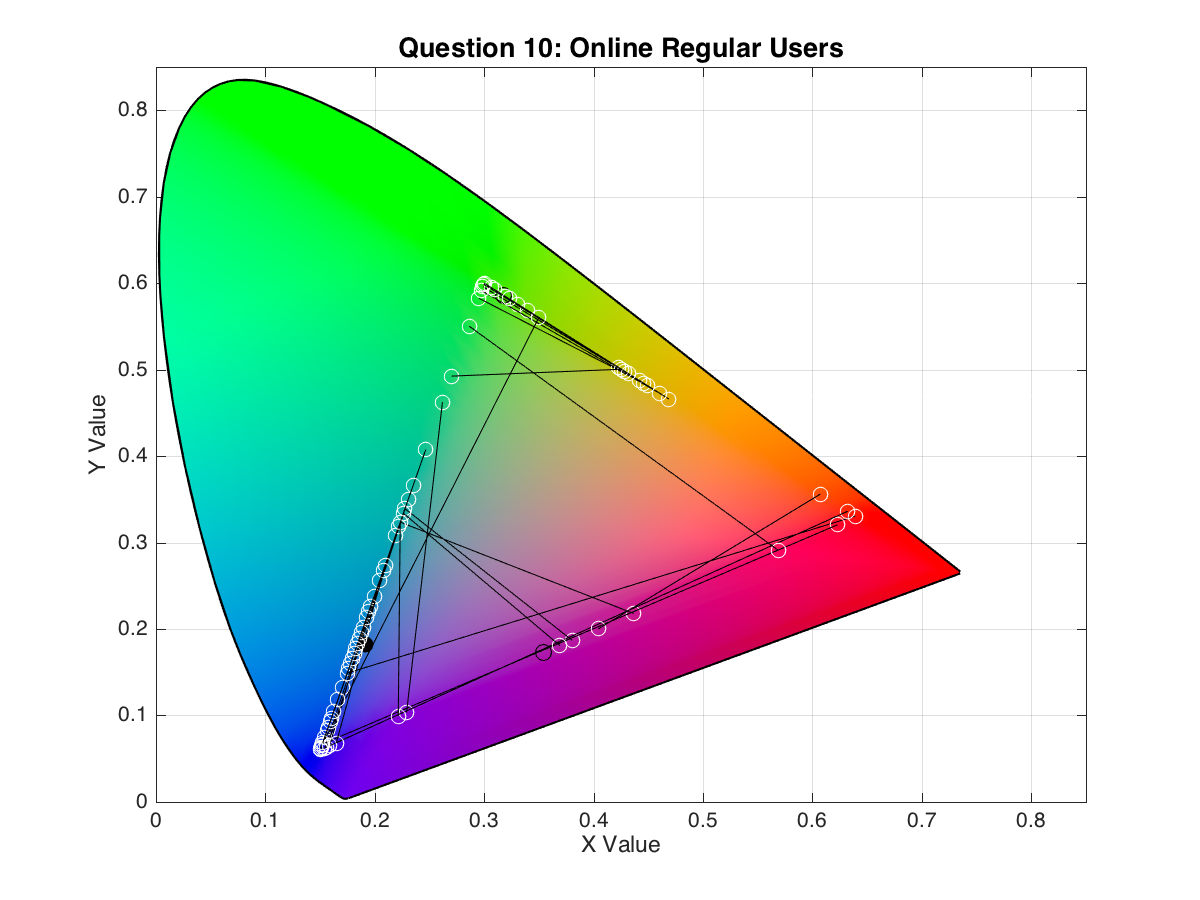
\includegraphics[width=\textwidth]{images/results/10_online_regularUsers.png}
    \caption[Online: Answers for Question 10, from regular users.]{Online: Question 10, Regular users.}
    \label{fig:onlineregular_10}
  \end{minipage}\hfill
  \begin{minipage}{0.48\textwidth}
    \centering
    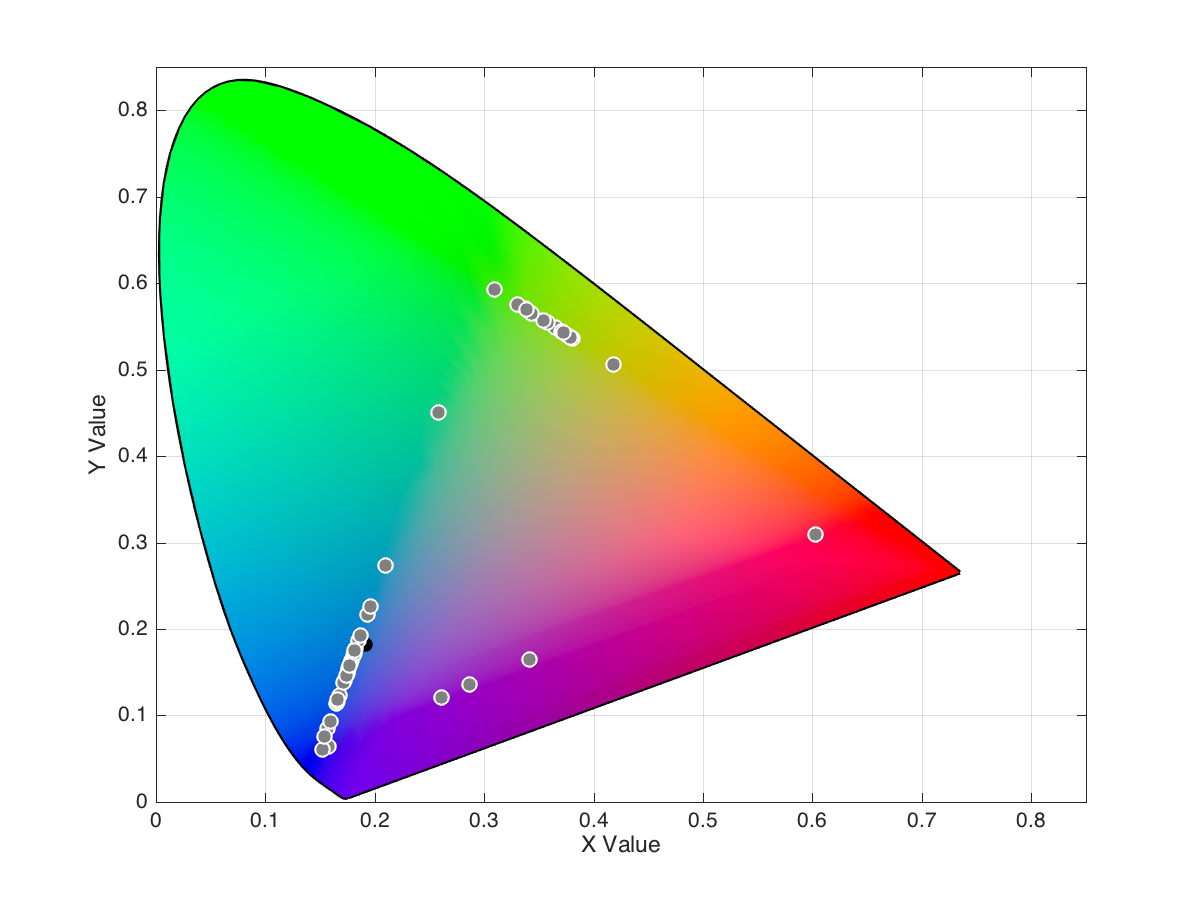
\includegraphics[width=\textwidth]{images/results/10_online_HSVresponses.png}
    \caption[Online: Answers for Question 10, from regular users, mixed in HSV Color Model.]{Online: Question 10, Regular users, mixed in HSV.}
    \label{fig:onlinehsvregular_10}
  \end{minipage}
  \vspace{-5pt}
\end{figure}
%
\paragraph{\ul{Question Eleven}}
%
This question has the second possible output from the blend of \ul{Green and Magenta colors}. Mean distances are dramatically lower for this question ($\overline{x} = 0.06$),
whilst the deviation of answers is also lower. However, there is an interesting feature: instead of believing in a Green-Magenta blending to produce Orange, \textbf{the users tend to use again Red and Yellow} as on question six,
which explains the low HSV mean value for question eleven.
%
Based on these results, we can conclude \textbf{the orange color is a strongly implemented color in mental models of our users}. The results from this question can be found in table
\ref{table:lab_q11_expected}. Once again, \textbf{these results are corroborated by the online users}, since a Wilcoxon Test show that there are no statistically significant differences between the laboratory
distances and online ones ($p < 0.05$).
%
\begin{table}[H]
  \resizebox{\textwidth}{!} {
  \begin{tabular}{lccccccccccccc}
    \hline
    \multicolumn{1}{c}{}                              &                                      & \multicolumn{2}{c}{Reference Pair}                   & \multicolumn{10}{c}{Possible Results}                                                                                                                                                                                                                                                                                        \\ \cline{3-14}
    \multicolumn{1}{c}{\multirow{-2}{*}{Question ID}} & \multirow{-2}{*}{Given Color}        & C1                       & C2                         & \multicolumn{2}{c}{HSV}                                        & \multicolumn{2}{c}{CIE-L*C*h*}                                 & \multicolumn{2}{c}{CMYK}                                       & \multicolumn{2}{c}{RGB}                                        & \multicolumn{2}{c}{CIE-L*a*b*}                                 \\ \hline
    \multicolumn{1}{c}{11}                             & \cellcolor[HTML]{FF8000}(49, 37, 5) & \multicolumn{1}{c|}{Green} & \multicolumn{1}{c|}{Magenta}  & \multicolumn{2}{c|}{\cellcolor[HTML]{FF8000}(49, 37, 5)}      & \multicolumn{2}{c|}{\cellcolor[HTML]{FF6F00}(47, 33, 4)}       & \multicolumn{2}{c|}{\cellcolor[HTML]{808080}{\color[HTML]{FFFFFF}(21, 22, 24)}}       & \multicolumn{2}{c|}{\cellcolor[HTML]{808080}{\color[HTML]{FFFFFF}(21, 22, 24)}}       & \multicolumn{2}{c|}{\cellcolor[HTML]{C9B2A2}(47, 48, 41)}       \\ \hline
                                                      & \multicolumn{1}{l}{}                 & \multicolumn{1}{l}{}     & \multicolumn{1}{l}{}       & \multicolumn{1}{c}{$\overline{x}$} & \multicolumn{1}{c}{$s$} & \multicolumn{1}{c}{$\overline{x}$} & \multicolumn{1}{c}{$s$} & \multicolumn{1}{c}{$\overline{x}$} & \multicolumn{1}{c}{$s$} & \multicolumn{1}{c}{$\overline{x}$} & \multicolumn{1}{c}{$s$} & \multicolumn{1}{c}{$\overline{x}$} & \multicolumn{1}{c}{$s$} \\ \hline
    \multicolumn{4}{l}{Distance to Objective - Laboratory}                                                                                           & \multicolumn{1}{|c}{\textbf{0.06}}       & \multicolumn{1}{c|}{0.09}    & \multicolumn{1}{|c}{0.14}       & \multicolumn{1}{c|}{0.12}    & \multicolumn{1}{|c}{0.13}       & \multicolumn{1}{c|}{0.03}    & \multicolumn{1}{|c}{0.18}       & \multicolumn{1}{c|}{0.04}    & \multicolumn{1}{|c}{0.14}       & \multicolumn{1}{c|}{0.03}    \\
    \multicolumn{4}{l}{Distance to Objective - Online}                                                                                               & \multicolumn{1}{|c}{\textbf{0.04}}        & \multicolumn{1}{c|}{0.06}    & \multicolumn{1}{|c}{0.12}        & \multicolumn{1}{c|}{0.10}    & \multicolumn{1}{|c}{0.14}       & \multicolumn{1}{c|}{0.02}    & \multicolumn{1}{|c}{0.19}        & \multicolumn{1}{c|}{0.02}    & \multicolumn{1}{|c}{0.15}       & \multicolumn{1}{c|}{0.01}    \\ \hline
    \end{tabular}}
  \caption[Question 11, with expected Results.]{Question 11: expected colors, possible results and statistics of distances to Objective.}
  \vspace{-5pt}
  \label{table:lab_q11_expected}
\end{table}
%
\paragraph{\ul{Question Twelve}}
%
It is observable that HSV Color Model presents, the lowest mean value for distance to ideal answer ($\overline{x} = 0.11$), whilst standard deviation for the CMYK Color Model provides the lowest value between both study environments
($s_{lab} = 0.04$, $s_{online} = 0.05$).
The results show that CIE-L*C*h* the worst-generating values Color Model; there is also the same tendency of RGB, CIE-L*a*b* and CMYK present closer values between each other. Evaluating the data with the Friedman Test, we can conclude that there are significant differences ($\chi^2 = 71.788$, $p < 0.05$)
between the color models; a Wilcoxon Analysis ($p < 0.05$) does reveal \textbf{there are significant difference between color models}: when analyzing the results for the tests between HSV and other
color models, it presents significant differences between all models except CMYK; the model which consistently presents the larger distances is CIE-L*C*h* against every color model, leading to
statistically significant differences with every other model. \par
%
Comparing the results of this question with number three, we can observe that the later has shorter values: HSV Color Model still presents the best mean values between questions.
The fact that question three has lower values, leads us to conclude that \textbf{mixing Red and Cyan to achieve this green tone is more similar with the users' expectations, than blending a Green and
Yellow color}. Figures \ref{fig:onlinehsvregular_3} and \ref{fig:onlinehsvregular_12} compare the results from both question three and twelve, blended in HSV (the model which yields the best results).
%
\begin{table}[H]
  \resizebox{\textwidth}{!} {
  \begin{tabular}{lccccccccccccc}
    \hline
    \multicolumn{1}{c}{}                              &                                      & \multicolumn{2}{c}{Reference Pair}                   & \multicolumn{10}{c}{Possible Results}                                                                                                                                                                                                                                                                                        \\ \cline{3-14}
    \multicolumn{1}{c}{\multirow{-2}{*}{Question ID}} & \multirow{-2}{*}{Given Color}        & C1                       & C2                         & \multicolumn{2}{c}{HSV}                                        & \multicolumn{2}{c}{CIE-L*C*h*}                                 & \multicolumn{2}{c}{CMYK}                                       & \multicolumn{2}{c}{RGB}                                        & \multicolumn{2}{c}{CIE-L*a*b*}                                 \\ \hline
    \multicolumn{1}{c}{12}                             & \cellcolor[HTML]{80FF00}(45, 76, 12) & \multicolumn{1}{c|}{Green} & \multicolumn{1}{c|}{Yellow}  & \multicolumn{2}{c|}{\cellcolor[HTML]{80FF00}(45, 76, 12)}      & \multicolumn{2}{c|}{\cellcolor[HTML]{B1FF00}(54, 81, 13)}       & \multicolumn{2}{c|}{\cellcolor[HTML]{80FF00}(45, 76, 12)}       & \multicolumn{2}{c|}{\cellcolor[HTML]{80FF00}(45, 76, 12)}       & \multicolumn{2}{c|}{\cellcolor[HTML]{AEFF00}(53, 81, 13)}       \\ \hline
                                                      & \multicolumn{1}{l}{}                 & \multicolumn{1}{l}{}     & \multicolumn{1}{l}{}       & \multicolumn{1}{c}{$\overline{x}$} & \multicolumn{1}{c}{$s$} & \multicolumn{1}{c}{$\overline{x}$} & \multicolumn{1}{c}{$s$} & \multicolumn{1}{c}{$\overline{x}$} & \multicolumn{1}{c}{$s$} & \multicolumn{1}{c}{$\overline{x}$} & \multicolumn{1}{c}{$s$} & \multicolumn{1}{c}{$\overline{x}$} & \multicolumn{1}{c}{$s$} \\ \hline
    \multicolumn{4}{l}{Distance to Objective - Laboratory}                                                                                           & \multicolumn{1}{|c}{\textbf{0.11}}       & \multicolumn{1}{c|}{0.13}    & \multicolumn{1}{|c}{0.23}       & \multicolumn{1}{c|}{0.07}    & \multicolumn{1}{|c}{0.13}       & \multicolumn{1}{c|}{0.04}    & \multicolumn{1}{|c}{0.15}       & \multicolumn{1}{c|}{0.08}    & \multicolumn{1}{|c}{0.17}       & \multicolumn{1}{c|}{0.07}    \\
    \multicolumn{4}{l}{Distance to Objective - Online}                                                                                               & \multicolumn{1}{|c}{\textbf{0.08}}        & \multicolumn{1}{c|}{0.11}    & \multicolumn{1}{|c}{0.24}        & \multicolumn{1}{c|}{0.06}    & \multicolumn{1}{|c}{0.12}       & \multicolumn{1}{c|}{0.05}    & \multicolumn{1}{|c}{0.13}        & \multicolumn{1}{c|}{0.09}    & \multicolumn{1}{|c}{0.15}       & \multicolumn{1}{c|}{0.09}    \\ \hline
    \end{tabular}}
  \caption[Question 12, with expected Results.]{Question 12: expected colors, possible results and statistics of distances to Objective.}
  \vspace{-5pt}
  \label{table:lab_q12_expected}
\end{table}
%
\begin{figure}[htbp]
  \centering
  \vspace{-15pt}
  \begin{minipage}{0.48\textwidth}
    \centering
    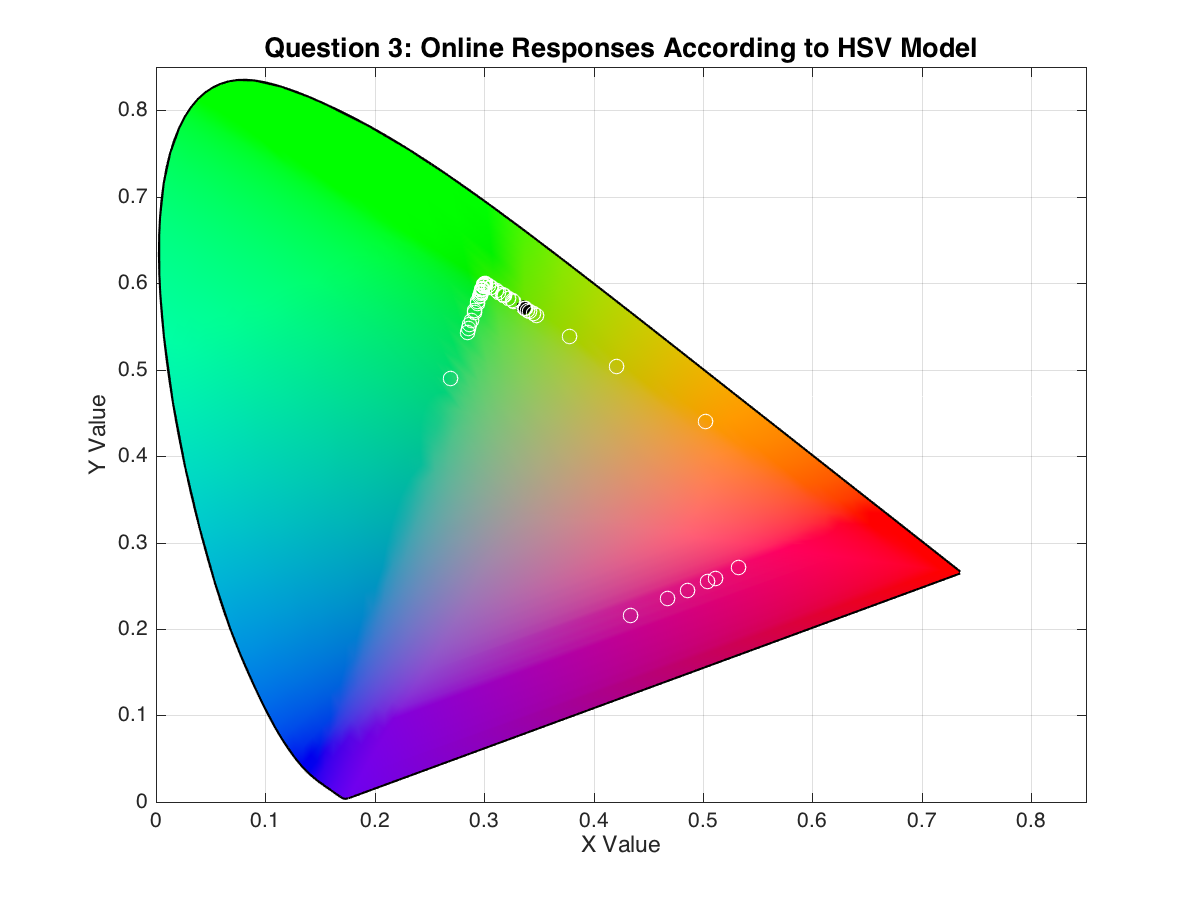
\includegraphics[width=\textwidth]{images/results/3_online_HSVresponses.png}
    \caption[Online: Answers for Question 3, from regular users, mixed in HSV Color Model.]{Online: Answers for Question 3, from regular users, mixed in HSV Color Model.}
    \label{fig:onlinehsvregular_3}
  \end{minipage}\hfill
  \begin{minipage}{0.48\textwidth}
    \centering
    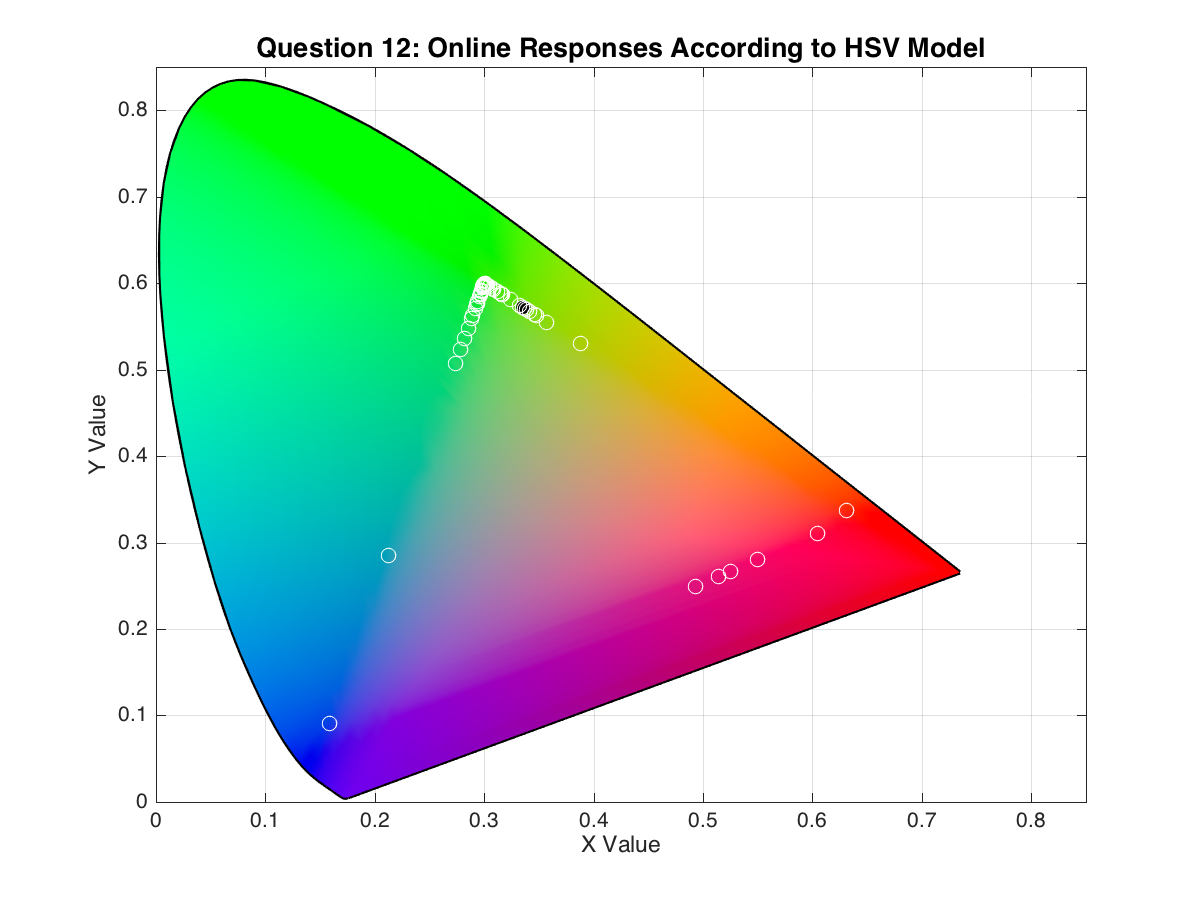
\includegraphics[width=\textwidth]{images/results/12_online_HSVresponses.png}
    \caption[Online: Answers for Question 12, from regular users, mixed in HSV Color Model.]{Online: Answers for Question 12, from regular users, mixed in HSV Color Model.}
    \label{fig:onlinehsvregular_12}
  \end{minipage}
  \vspace{-5pt}
\end{figure}
%
\paragraph{\ul{Question Thirteen}}
%
It is interesting to see CIE-L*C*h* overcoming the lowest result in the laboratory environment, against other color models which regularly had best results in previous questions; however, these results are not consistent with the online users, which indicated responses closer to the RGB Color Model
($s_{online} = 0.13$).
Analyzing the laboratory results, it shows that HSV is the worst-generating values Color Model, having the higher mean value ($\overline{x}_{HSV} = 0.27$) of all models. When comparing it to the online dataset,
HSV, CMYK and CIE-L*a*b* have all the same mean values. Evaluating the data with the Friedman Test, we can conclude that there are significant differences ($\chi^2 = 38.993$, $p < 0.05$)
between the color models on the laboratory results; a Wilcoxon Analysis ($p < 0.05$) does reveal \textbf{there are significant difference between color models}: when analyzing the results for the tests between HSV and other
color models, it presents significant differences between all models except CIE-L*C*h*. \par
%
Comparing the results of this question with number ten, we can observe that this question has shorter HSV value; however we know that HSV was not the lowest mean value on question thirteen
These results leads us to conclude that \textbf{there are insufficient values to ascertain the best color model to achieve this blue tone}. Further studies are required to unveil the
appropriate color model and clarify this matter. Figures \ref{fig:onlinehsvregular_10} and \ref{fig:onlinehsvregular_13} compare the results from both question ten and thirteen, blended in HSV and RGB respectively. \par
%
Moreover, these results are \textbf{not} corroborated by the online users, since a Wilcoxon Test show that there are indeed statistically significant differences between the laboratory distances
and online ones ($p < 0.05$): namely between the CMYK distance values ($p = 0.041$) and RGB ($p = 0.005$).
%
\begin{table}[H]
  \resizebox{\textwidth}{!} {
  \begin{tabular}{lccccccccccccc}
    \hline
    \multicolumn{1}{c}{}                              &                                      & \multicolumn{2}{c}{Reference Pair}                   & \multicolumn{10}{c}{Possible Results}                                                                                                                                                                                                                                                                                        \\ \cline{3-14}
    \multicolumn{1}{c}{\multirow{-2}{*}{Question ID}} & \multirow{-2}{*}{Given Color}        & C1                       & C2                         & \multicolumn{2}{c}{HSV}                                        & \multicolumn{2}{c}{CIE-L*C*h*}                                 & \multicolumn{2}{c}{CMYK}                                       & \multicolumn{2}{c}{RGB}                                        & \multicolumn{2}{c}{CIE-L*a*b*}                                 \\ \hline
    \multicolumn{1}{c}{13}                             & \cellcolor[HTML]{0080FF}{\color[HTML]{FFFFFF}(26, 23, 98)} & \multicolumn{1}{c|}{Blue} & \multicolumn{1}{c|}{Cyan}  & \multicolumn{2}{c|}{\cellcolor[HTML]{0080FF}{\color[HTML]{FFFFFF}(26, 23, 98)}}      & \multicolumn{2}{c|}{\cellcolor[HTML]{00ACFF}(33, 37, 100)}       & \multicolumn{2}{c|}{\cellcolor[HTML]{0080FF}{\color[HTML]{FFFFFF}(26, 23, 98)}}       & \multicolumn{2}{c|}{\cellcolor[HTML]{0080FF}{\color[HTML]{FFFFFF}(26, 23, 98)}}       & \multicolumn{2}{c|}{\cellcolor[HTML]{5792FF}{\color[HTML]{FFFFFF}(32, 30, 99)}}       \\ \hline
                                                      & \multicolumn{1}{l}{}                 & \multicolumn{1}{l}{}     & \multicolumn{1}{l}{}       & \multicolumn{1}{c}{$\overline{x}$} & \multicolumn{1}{c}{$s$} & \multicolumn{1}{c}{$\overline{x}$} & \multicolumn{1}{c}{$s$} & \multicolumn{1}{c}{$\overline{x}$} & \multicolumn{1}{c}{$s$} & \multicolumn{1}{c}{$\overline{x}$} & \multicolumn{1}{c}{$s$} & \multicolumn{1}{c}{$\overline{x}$} & \multicolumn{1}{c}{$s$} \\ \hline
    \multicolumn{4}{l}{Distance to Objective - Laboratory}                                                                                           & \multicolumn{1}{|c}{0.27}       & \multicolumn{1}{c|}{0.16}    & \multicolumn{1}{|c}{\textbf{0.17}}       & \multicolumn{1}{c|}{0.10}    & \multicolumn{1}{|c}{0.19}       & \multicolumn{1}{c|}{0.13}    & \multicolumn{1}{|c}{0.25}       & \multicolumn{1}{c|}{0.16}    & \multicolumn{1}{|c}{0.23}       & \multicolumn{1}{c|}{0.12}    \\
    \multicolumn{4}{l}{Distance to Objective - Online}                                                                                               & \multicolumn{1}{|c}{0.14}        & \multicolumn{1}{c|}{0.16}    & \multicolumn{1}{|c}{0.20}        & \multicolumn{1}{c|}{0.09}    & \multicolumn{1}{|c}{0.14}       & \multicolumn{1}{c|}{0.11}    & \multicolumn{1}{|c}{\textbf{0.13}}        & \multicolumn{1}{c|}{0.15}    & \multicolumn{1}{|c}{0.14}       & \multicolumn{1}{c|}{0.11}    \\ \hline
    \end{tabular}}
  \caption[Question 13, with expected Results.]{Question 13: expected colors, possible results and statistics of distances to Objective.}
  \vspace{-5pt}
  \label{table:lab_q13_expected}
\end{table}
%
\begin{figure}[htbp]
  \centering
  \vspace{-15pt}
  \begin{minipage}{0.48\textwidth}
    \centering
    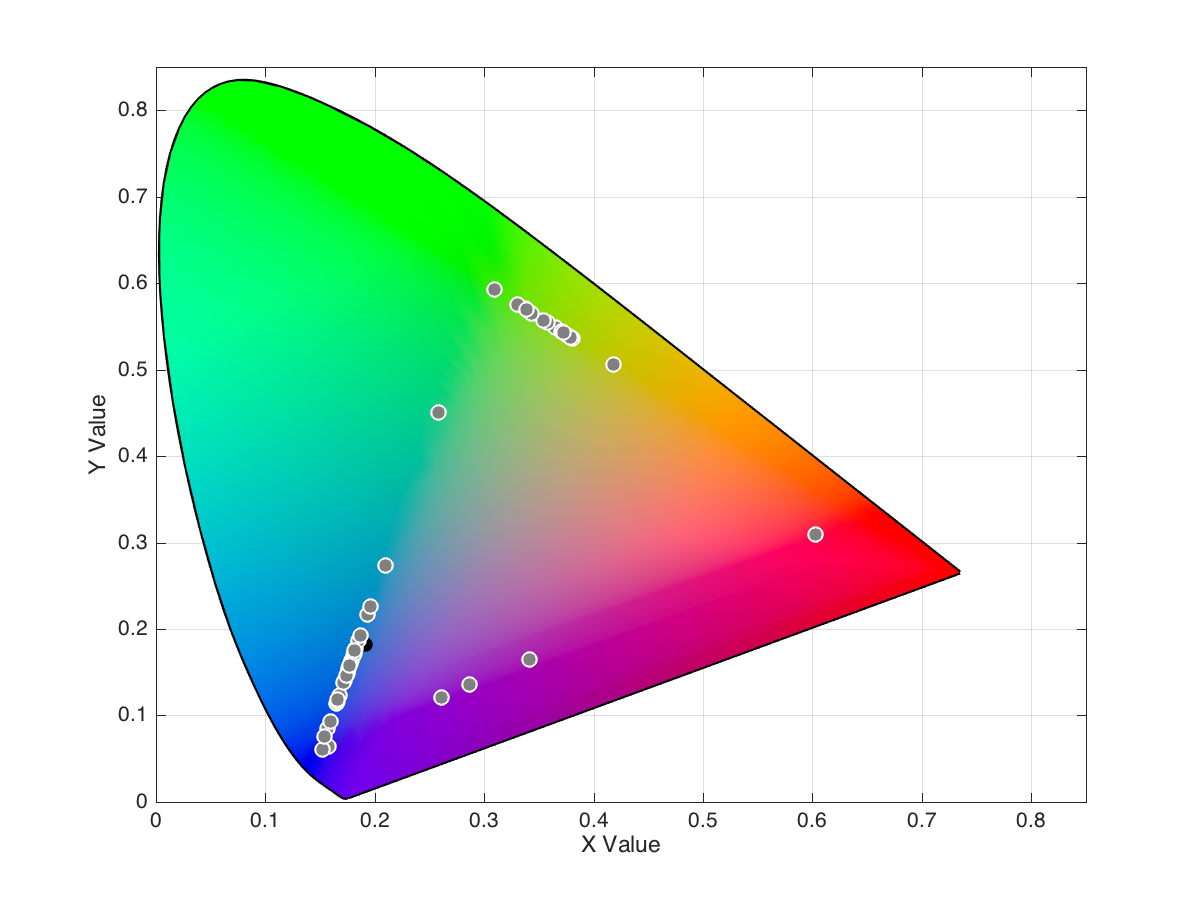
\includegraphics[width=\textwidth]{images/results/10_online_HSVresponses.png}
    \caption[Online: Answers for Question 10, from regular users, mixed in HSV Color Model.]{Online: Answers for Question 10, from regular users, mixed in HSV Color Model.}
    \label{fig:onlinehsvregular_10}
  \end{minipage}\hfill
  \begin{minipage}{0.48\textwidth}
    \centering
    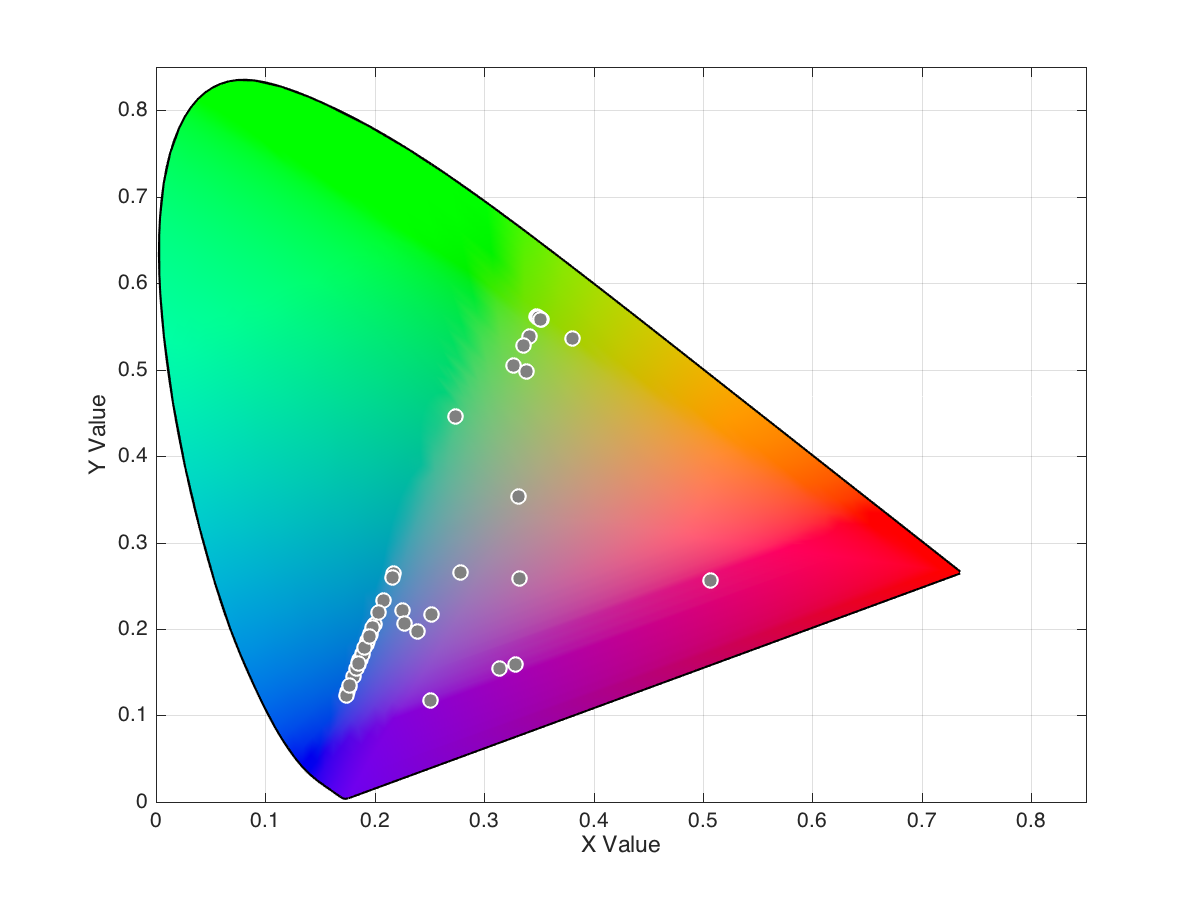
\includegraphics[width=\textwidth]{images/results/13_online_RGBresponses.png}
    \caption[Online: Answers for Question 13, from regular users, mixed in RGB Color Model.]{Online: Answers for Question 13, from regular users, mixed in RGB Color Model.}
    \label{fig:onlinehsvregular_13}
  \end{minipage}
  \vspace{-5pt}
\end{figure}
%
\paragraph{\ul{Question Fourteen}}
%
It is observable that CMYK Color Model presents, the lowest mean value for distance to ideal answer ($\overline{x} = 0.10$ laboratory, and $\overline{x} = 0.09$ online), whilst standard deviation for the CMYK Color Model is also the
lowest between both study environments presenting exactly the same value.
The results show that CIE-L*C*h* the worst-generating values Color Model having, by far, the higher mean value of all models across study environments ($\overline{x} = 0.30$). There is also the same tendency of RGB,
CIE-L*a*b* and HSV present closer values between each other. Evaluating the data with the Friedman Test, we can conclude that there are significant differences ($\chi^2 = 51.726$, $p < 0.05$)
between the color models; a Wilcoxon Analysis ($p < 0.05$) does reveal there are no significant difference between color models: mostly, the significant differences reside in CIE-L*C*h*, when
compared with HSV, CMYK and CIE-L*a*b*. \par
%
\begin{table}[H]
  \resizebox{\textwidth}{!} {
  \begin{tabular}{lccccccccccccc}
    \hline
    \multicolumn{1}{c}{}                              &                                      & \multicolumn{2}{c}{Reference Pair}                   & \multicolumn{10}{c}{Possible Results}                                                                                                                                                                                                                                                                                        \\ \cline{3-14}
    \multicolumn{1}{c}{\multirow{-2}{*}{Question ID}} & \multirow{-2}{*}{Given Color}        & C1                       & C2                         & \multicolumn{2}{c}{HSV}                                        & \multicolumn{2}{c}{CIE-L*C*h*}                                 & \multicolumn{2}{c}{CMYK}                                       & \multicolumn{2}{c}{RGB}                                        & \multicolumn{2}{c}{CIE-L*a*b*}                                 \\ \hline
    \multicolumn{1}{c}{14}                             & \cellcolor[HTML]{8000FF}{\color[HTML]{FFFFFF}(27, 12, 95)} & \multicolumn{1}{c|}{Blue} & \multicolumn{1}{c|}{Magenta}  & \multicolumn{2}{c|}{\cellcolor[HTML]{8000FF}{\color[HTML]{FFFFFF}(27, 12, 95)}}      & \multicolumn{2}{c|}{\cellcolor[HTML]{B000FF}{\color[HTML]{FFFFFF}(36, 16, 96)}}       & \multicolumn{2}{c|}{\cellcolor[HTML]{8000FF}{\color[HTML]{FFFFFF}(27, 12, 95)}}       & \multicolumn{2}{c|}{\cellcolor[HTML]{8000FF}{\color[HTML]{FFFFFF}(27, 12, 95)}}       & \multicolumn{2}{c|}{\cellcolor[HTML]{AB00FF}{\color[HTML]{FFFFFF}(35, 16, 96)}}       \\ \hline
                                                      & \multicolumn{1}{l}{}                 & \multicolumn{1}{l}{}     & \multicolumn{1}{l}{}       & \multicolumn{1}{c}{$\overline{x}$} & \multicolumn{1}{c}{$s$} & \multicolumn{1}{c}{$\overline{x}$} & \multicolumn{1}{c}{$s$} & \multicolumn{1}{c}{$\overline{x}$} & \multicolumn{1}{c}{$s$} & \multicolumn{1}{c}{$\overline{x}$} & \multicolumn{1}{c}{$s$} & \multicolumn{1}{c}{$\overline{x}$} & \multicolumn{1}{c}{$s$} \\ \hline
    \multicolumn{4}{l}{Distance to Objective - Laboratory}                                                                                           & \multicolumn{1}{|c}{0.12}       & \multicolumn{1}{c|}{0.14}    & \multicolumn{1}{|c}{0.30}       & \multicolumn{1}{c|}{0.09}    & \multicolumn{1}{|c}{\textbf{0.10}}       & \multicolumn{1}{c|}{0.05}    & \multicolumn{1}{|c}{0.13}       & \multicolumn{1}{c|}{0.13}    & \multicolumn{1}{|c}{0.13}       & \multicolumn{1}{c|}{0.09}    \\
    \multicolumn{4}{l}{Distance to Objective - Online}                                                                                               & \multicolumn{1}{|c}{0.10}        & \multicolumn{1}{c|}{0.12}    & \multicolumn{1}{|c}{0.29}        & \multicolumn{1}{c|}{0.13}    & \multicolumn{1}{|c}{\textbf{0.09}}       & \multicolumn{1}{c|}{0.05}    & \multicolumn{1}{|c}{0.11}        & \multicolumn{1}{c|}{0.12}    & \multicolumn{1}{|c}{0.12}       & \multicolumn{1}{c|}{0.09}    \\ \hline
    \end{tabular}}
  \caption[Question 14, with expected Results.]{Question 14: expected colors, possible results and statistics of distances to Objective.}
  \vspace{-5pt}
  \label{table:lab_q14_expected}
\end{table}
%
Evaluating this question, it is possible to affirm that \textbf{CMYK has the best results when mixing purple, a color derived from magenta}, due to the commitment between the mean value and standard deviation, which
could be justified by the fact that \textbf{magenta is a primitive from such model, combined with the indication shown throughout the study to demonstrate a subtractive mental model of color}.
\textbf{These results are corroborated by the online users}, since a Wilcoxon Test show that there are no statistically significant differences between the laboratory distances and online ones ($p < 0.05$).
%
\paragraph{\ul{Question Fifteen}}
%
This question also presented a repeated color: this green shade is equal to the one presented in question nine, therefore its results are interesting to compare with this question.
The colors were blended and the mean values over distances were calculated: it is observable that CMYK Color Model presents the lowest mean value
for distance to ideal answer ($\overline{x} = 0.06$); its standard deviation is also the lowest between both study environments ($s = 0.03$). Though, it is important to analyze this result: since we
are mixing opposite colors, both CMYK and RGB generate a neutral color, which means that the closer the users' answers are from the ideal answers (Blue and Yellow), the shorter the distance on these color
models, and greyer the shade. \textbf{This value, in fact, supports the result of HSV Color} ($\overline{x}_{HSV} = 0.09$), which is very acceptable since the answer pairs are very close to the expected one. \par
%
Running the Friedman Test, we can conclude that there are significant differences ($\chi^2 = 63.068$, $p < 0.05$) between the color models; a Wilcoxon Analysis ($p < 0.05$) reveals that
there are statistically different results among all color models, except for \ul{HSV and RGB} and \ul{HSV and CIE-L*a*b*}, which do not have statistically significant differences.
Comparing the results of this question with number nine, we can observe that this question has shorter values: HSV Color Model still presents the best mean values between questions, and deviations of question 15
answers are lower for all models against question 9. This fact leads us to conclude that \textbf{mixing Blue and Cyan to achieve this green shade is more similar with the users' expectations, than blending a Green and
Cyan color}. Figures \ref{fig:onlinehsvregular_9} and \ref{fig:onlinehsvregular_15} compare the results from both question nine and fifteen, blended in HSV (the model which yields the best results). \par
%
HSV has statistically different results from other color models, therefore concluding that \textbf{HSV has the best solution for this blending}. \textbf{The laboratory results are corroborated by the online ones}, since a Wilcoxon Test show that there
are no statistically significant differences between the laboratory distances and online ($p < 0.05$).\par
%
\begin{table}[H]
  \resizebox{\textwidth}{!} {
  \begin{tabular}{lccccccccccccc}
    \hline
    \multicolumn{1}{c}{}                              &                                      & \multicolumn{2}{c}{Reference Pair}                   & \multicolumn{10}{c}{Possible Results}                                                                                                                                                                                                                                                                                        \\ \cline{3-14}
    \multicolumn{1}{c}{\multirow{-2}{*}{Question ID}} & \multirow{-2}{*}{Given Color}        & C1                       & C2                         & \multicolumn{2}{c}{HSV}                                        & \multicolumn{2}{c}{CIE-L*C*h*}                                 & \multicolumn{2}{c}{CMYK}                                       & \multicolumn{2}{c}{RGB}                                        & \multicolumn{2}{c}{CIE-L*a*b*}                                 \\ \hline
    \multicolumn{1}{c}{15}                             & \cellcolor[HTML]{00FF80}(40, 73, 32) & \multicolumn{1}{c|}{Blue} & \multicolumn{1}{c|}{Yellow}  & \multicolumn{2}{c|}{\cellcolor[HTML]{00FF80}(40, 73, 32)}      & \multicolumn{2}{c|}{\cellcolor[HTML]{FF0050}(43, 22, 10)}       & \multicolumn{2}{c|}{\cellcolor[HTML]{808080}{\color[HTML]{FFFFFF}(21, 22, 24)}}       & \multicolumn{2}{c|}{\cellcolor[HTML]{808080}{\color[HTML]{FFFFFF}(21, 22, 24)}}       & \multicolumn{2}{c|}{\cellcolor[HTML]{CA8AAA}(41, 34, 42)}       \\ \hline
                                                      & \multicolumn{1}{l}{}                 & \multicolumn{1}{l}{}     & \multicolumn{1}{l}{}       & \multicolumn{1}{c}{$\overline{x}$} & \multicolumn{1}{c}{$s$} & \multicolumn{1}{c}{$\overline{x}$} & \multicolumn{1}{c}{$s$} & \multicolumn{1}{c}{$\overline{x}$} & \multicolumn{1}{c}{$s$} & \multicolumn{1}{c}{$\overline{x}$} & \multicolumn{1}{c}{$s$} & \multicolumn{1}{c}{$\overline{x}$} & \multicolumn{1}{c}{$s$} \\ \hline
    \multicolumn{4}{l}{Distance to Objective - Laboratory}                                                                                           & \multicolumn{1}{|c}{0.09}       & \multicolumn{1}{c|}{0.04}    & \multicolumn{1}{|c}{0.30}       & \multicolumn{1}{c|}{0.08}    & \multicolumn{1}{|c}{\textbf{0.06}}       & \multicolumn{1}{c|}{0.03}    & \multicolumn{1}{|c}{0.11}       & \multicolumn{1}{c|}{0.05}    & \multicolumn{1}{|c}{0.13}       & \multicolumn{1}{c|}{0.06}    \\
    \multicolumn{4}{l}{Distance to Objective - Online}                                                                                               & \multicolumn{1}{|c}{0.11}        & \multicolumn{1}{c|}{0.08}    & \multicolumn{1}{|c}{0.30}        & \multicolumn{1}{c|}{0.07}    & \multicolumn{1}{|c}{\textbf{0.06}}       & \multicolumn{1}{c|}{0.03}    & \multicolumn{1}{|c}{0.11}        & \multicolumn{1}{c|}{0.04}    & \multicolumn{1}{|c}{0.13}       & \multicolumn{1}{c|}{0.06}    \\ \hline
    \end{tabular}}
  \caption[Question 15, with expected Results.]{Question 15: expected colors, possible results and statistics of distances to Objective.}
  \vspace{-5pt}
  \label{table:lab_q15_expected}
\end{table}
%
\begin{figure}[htbp]
  \centering
  \vspace{-15pt}
  \begin{minipage}{0.48\textwidth}
    \centering
    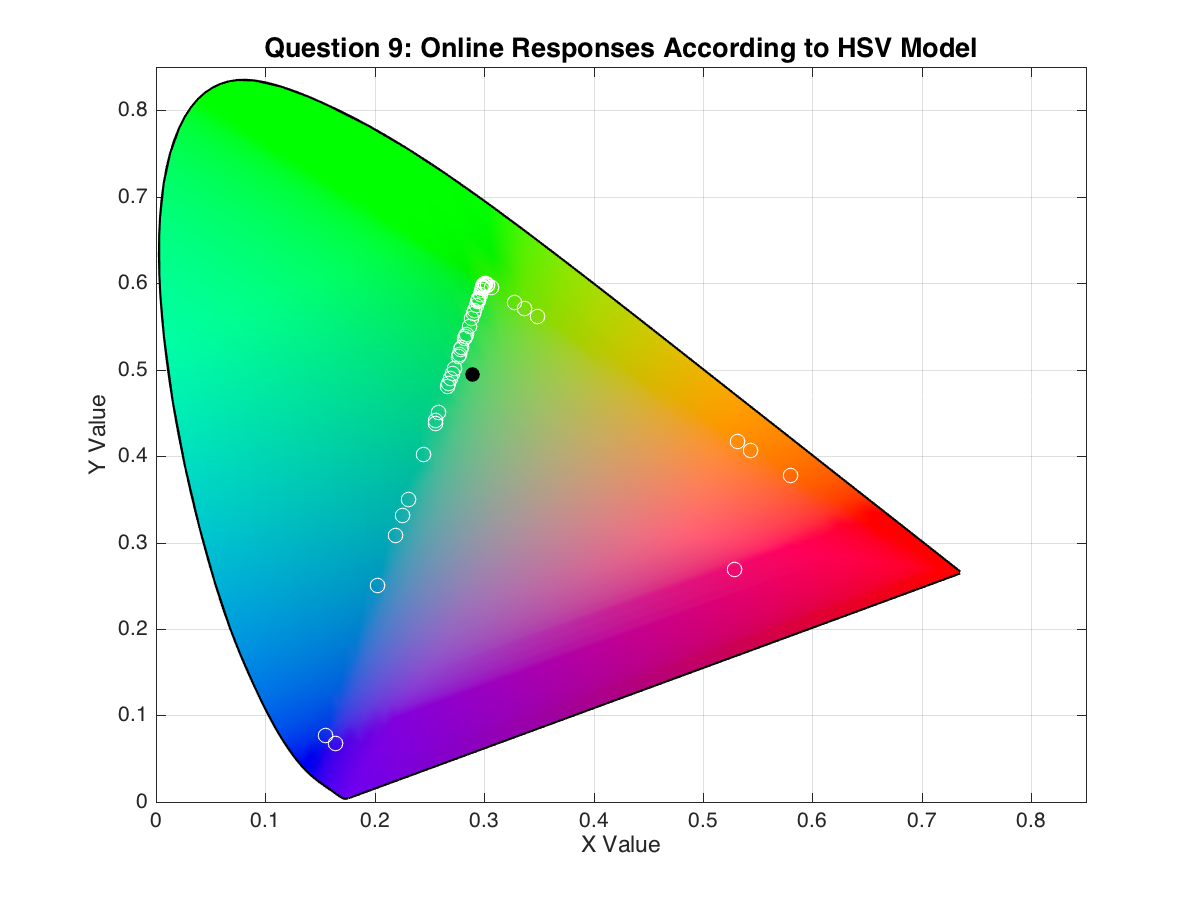
\includegraphics[width=\textwidth]{images/results/9_online_HSVresponses.png}
    \caption[Online: Answers for Question 9, from regular users, mixed in HSV Color Model.]{Online: Answers for Question 9, from regular users, mixed in HSV Color Model.}
    \label{fig:onlinehsvregular_9}
  \end{minipage}\hfill
  \begin{minipage}{0.48\textwidth}
    \centering
    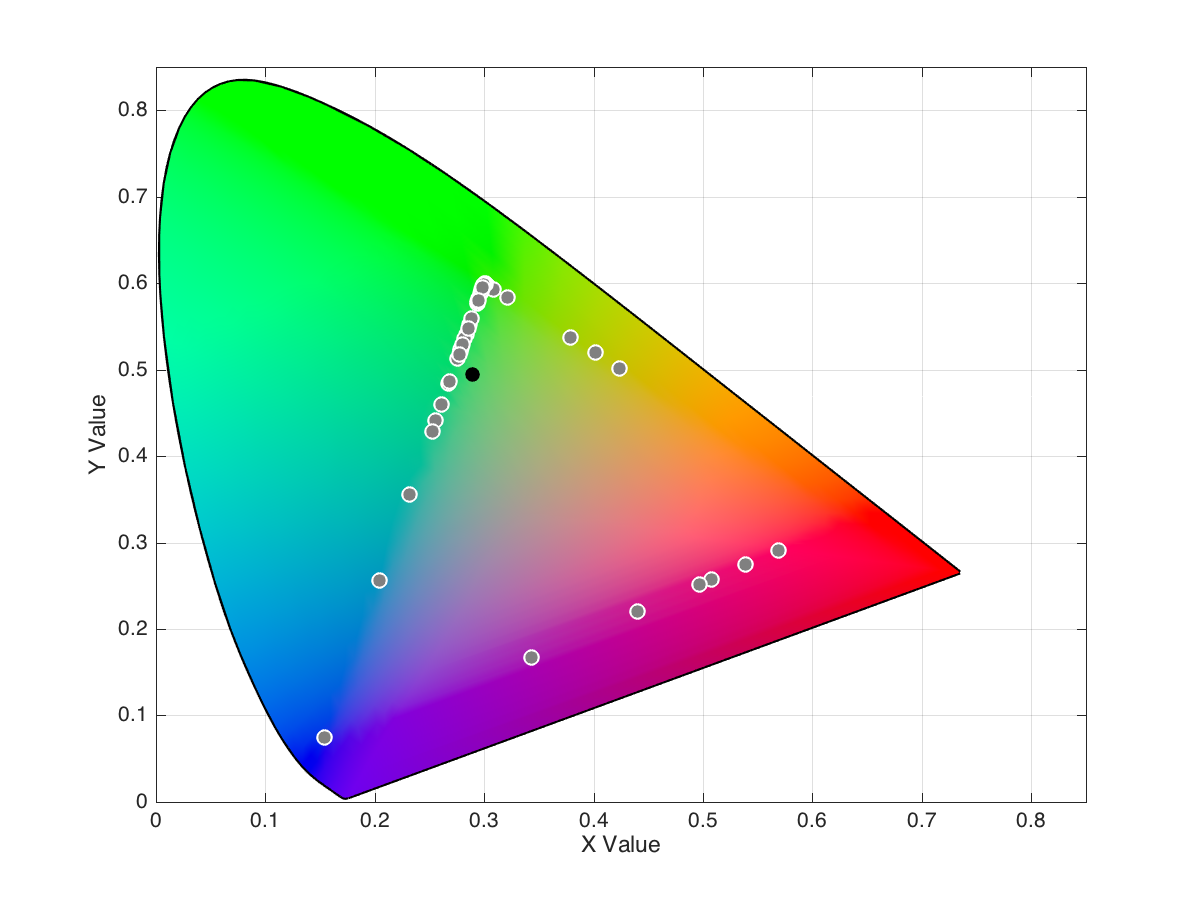
\includegraphics[width=\textwidth]{images/results/15_online_HSVresponses.png}
    \caption[Online: Answers for Question 15, from regular users, mixed in HSV Color Model.]{Online: Answers for Question 15, from regular users, mixed in HSV Color Model.}
    \label{fig:onlinehsvregular_15}
  \end{minipage}
  \vspace{-5pt}
\end{figure}
%
\paragraph{\ul{Question Sixteen}}
%
Comparing the results for the HSV Color Model of both question 15 and 16, mean distances are largely high for question 16
($\overline{x}_{lab} = 0.21$, $\overline{x}_{online} = 0.19$), whilst the deviation of answers is also lower in question 15.
Whilst the color presented was fairly similar with Magenta, the users tended to answer with Red-Blue pair of colors (which, as seen on question two, produces magenta according
to the HSV Color Model). \par
%
Based on these results, corroborated by the online users by a Wilcoxon Test with no significant differences ($p < 0.05$), we can conclude that \textbf{blending Blue and Yellow, according to users' mental model of color, produces Green instead of Magenta}. It is also
possible to conclude that \textbf{to produce Magenta, according to user's mental model of color, it is needed to blend Red and Blue}. The results from
this question can be found in Table \ref{table:lab_q16_expected}. These differences can be seen on Figures \ref{fig:onlineregular_16} and \ref{fig:onlinehsvregular_16}, which largely
demonstrate the placement of answer-pairs, and the pairs blended in HSV Color Model.
%
\begin{table}[H]
  \resizebox{\textwidth}{!} {
  \begin{tabular}{lccccccccccccc}
    \hline
    \multicolumn{1}{c}{}                              &                                      & \multicolumn{2}{c}{Reference Pair}                   & \multicolumn{10}{c}{Possible Results}                                                                                                                                                                                                                                                                                        \\ \cline{3-14}
    \multicolumn{1}{c}{\multirow{-2}{*}{Question ID}} & \multirow{-2}{*}{Given Color}        & C1                       & C2                         & \multicolumn{2}{c}{HSV}                                        & \multicolumn{2}{c}{CIE-L*C*h*}                                 & \multicolumn{2}{c}{CMYK}                                       & \multicolumn{2}{c}{RGB}                                        & \multicolumn{2}{c}{CIE-L*a*b*}                                 \\ \hline
    \multicolumn{1}{c}{16}                             & \cellcolor[HTML]{FF007F}{\color[HTML]{FFFFFF}(45, 23, 22)} & \multicolumn{1}{c|}{Blue} & \multicolumn{1}{c|}{Yellow}  & \multicolumn{2}{c|}{\cellcolor[HTML]{FF007F}{\color[HTML]{FFFFFF}(45, 23, 22)}}      & \multicolumn{2}{c|}{\cellcolor[HTML]{FF0050}{\color[HTML]{FFFFFF}(43, 22, 10)}}       & \multicolumn{2}{c|}{\cellcolor[HTML]{808080}{\color[HTML]{FFFFFF}(21, 22, 24)}}       & \multicolumn{2}{c|}{\cellcolor[HTML]{808080}{\color[HTML]{FFFFFF}(21, 22, 24)}}       & \multicolumn{2}{c|}{\cellcolor[HTML]{CA8AAA}(41, 34, 42)}       \\ \hline
                                                      & \multicolumn{1}{l}{}                 & \multicolumn{1}{l}{}     & \multicolumn{1}{l}{}       & \multicolumn{1}{c}{$\overline{x}$} & \multicolumn{1}{c}{$s$} & \multicolumn{1}{c}{$\overline{x}$} & \multicolumn{1}{c}{$s$} & \multicolumn{1}{c}{$\overline{x}$} & \multicolumn{1}{c}{$s$} & \multicolumn{1}{c}{$\overline{x}$} & \multicolumn{1}{c}{$s$} & \multicolumn{1}{c}{$\overline{x}$} & \multicolumn{1}{c}{$s$} \\ \hline
    \multicolumn{4}{l}{Distance to Objective - Laboratory}                                                                                           & \multicolumn{1}{|c}{0.21}       & \multicolumn{1}{c|}{0.10}    & \multicolumn{1}{|c}{0.22}       & \multicolumn{1}{c|}{0.12}    & \multicolumn{1}{|c}{\textbf{0.10}}       & \multicolumn{1}{c|}{0.05}    & \multicolumn{1}{|c}{0.16}       & \multicolumn{1}{c|}{0.07}    & \multicolumn{1}{|c}{0.12}       & \multicolumn{1}{c|}{0.08}    \\
    \multicolumn{4}{l}{Distance to Objective - Online}                                                                                               & \multicolumn{1}{|c}{0.19}        & \multicolumn{1}{c|}{0.12}    & \multicolumn{1}{|c}{0.17}        & \multicolumn{1}{c|}{0.09}    & \multicolumn{1}{|c}{\textbf{0.10}}       & \multicolumn{1}{c|}{0.06}    & \multicolumn{1}{|c}{0.15}        & \multicolumn{1}{c|}{0.07}    & \multicolumn{1}{|c}{0.11}       & \multicolumn{1}{c|}{0.06}    \\ \hline
    \end{tabular}}
  \caption[Question 16, with expected Results.]{Question 16: expected colors, possible results and statistics of distances to Objective.}
  \vspace{-5pt}
  \label{table:lab_q16_expected}
\end{table}
%
\begin{figure}[htbp]
  \centering
  \vspace{-15pt}
  \begin{minipage}{0.48\textwidth}
    \centering
    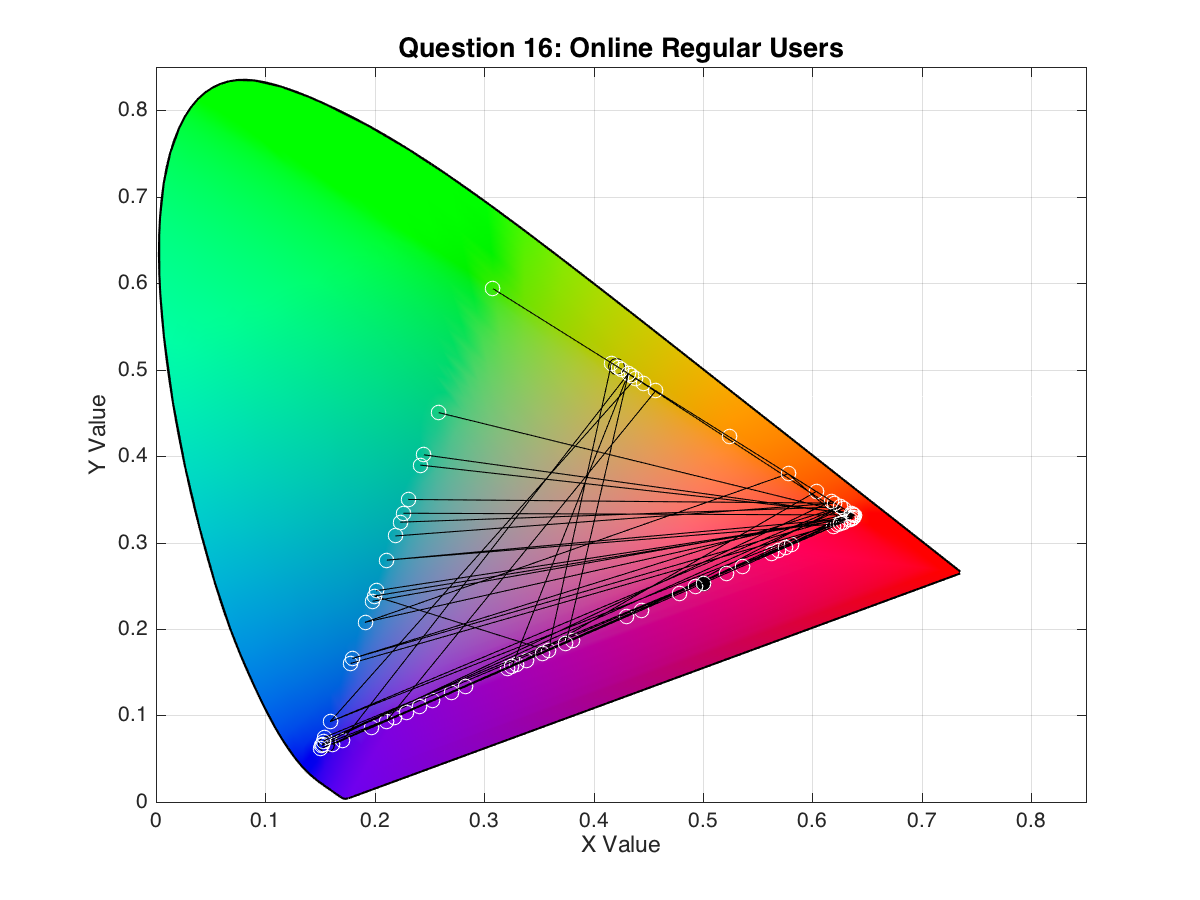
\includegraphics[width=\textwidth]{images/results/16_online_regularUsers.png}
    \caption[Online: Answers for Question 16, from regular users.]{Online: Answers for Question 16, from regular users.}
    \label{fig:onlineregular_16}
  \end{minipage}\hfill
  \begin{minipage}{0.48\textwidth}
    \centering
    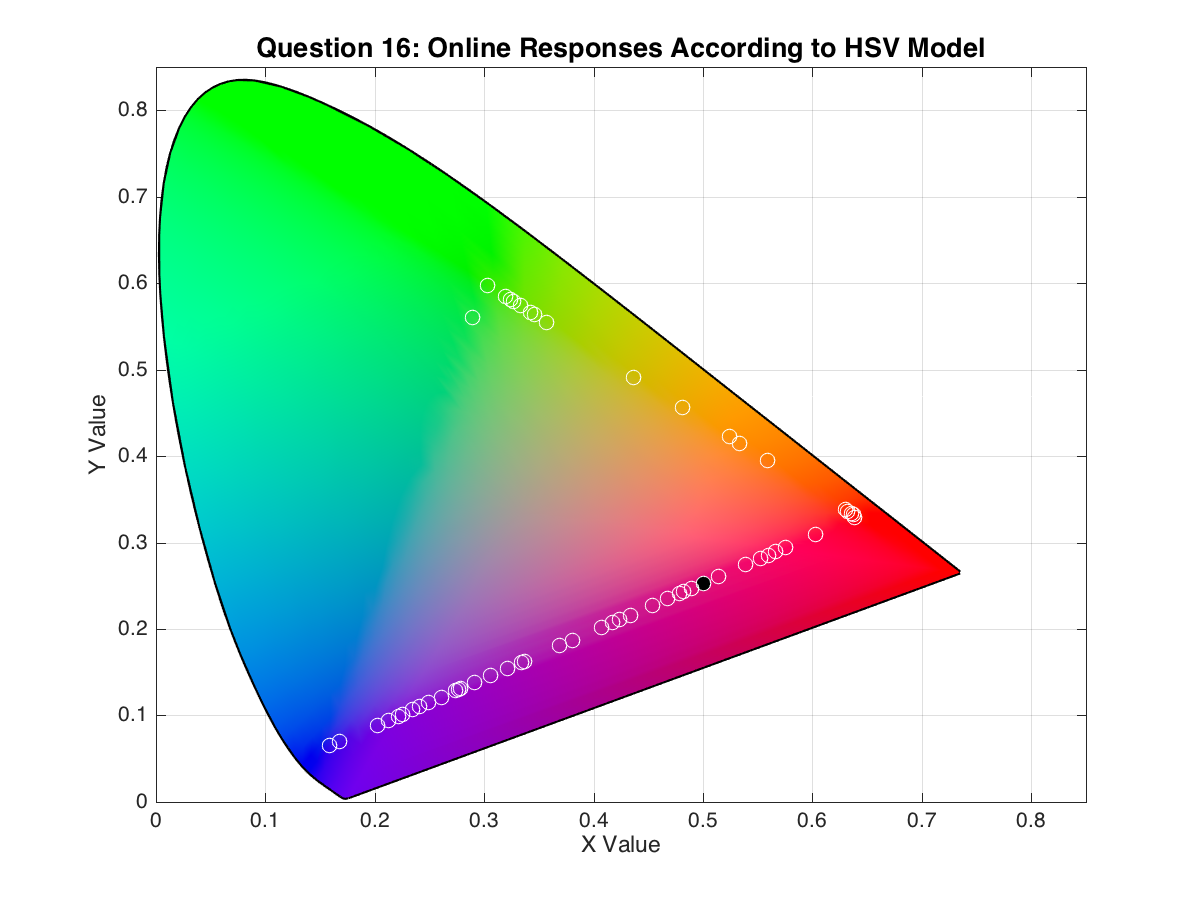
\includegraphics[width=\textwidth]{images/results/16_online_HSVresponses.png}
    \caption[Online: Answers for Question 16, from regular users, mixed in HSV Color Model.]{Online: Answers for Question 16, from regular users, mixed in HSV Color Model.}
    \label{fig:onlinehsvregular_16}
  \end{minipage}
  \vspace{-5pt}
\end{figure}
%
\paragraph{\ul{Question Seventeen}}
%
Finally, the colors for this last question were blended: it is observable that CMYK Color Model presents the lowest mean value for distance to ideal answer ($\overline{x} = 0.05$
laboratory, and $\overline{x} = 0.05$ online), whilst standard deviation for the CMYK Color Model is also the lowest between both study environments presenting exactly the same value.
The results show that CIE-L*C*h* the worst-generating values Color Model having the higher mean value of all models across study environments ($\overline{x} = 0.16$), which is consistent with the
entire user study. There is also the tendency of RGB and CIE-L*a*b* to present closer values between each other. Evaluating the data with the Friedman Test, we can conclude that there are significant
differences ($\chi^2 = 86.654$, $p < 0.05$) between the color models; a Wilcoxon Analysis ($p < 0.05$) does reveal there are clearly significant difference between color models: mostly, every color model
has significant differences between each other, except for HSV-CMYK, and RGB-CIE-L*a*b* which in fact present no statistically significant differences. \par
%
It is possible to affirm that \textbf{CMYK has the best results when cyan and yellow}, which could be justified by the fact that \textbf{cyan and yellow are primitives from such model, combined with the indication shown throughout the study to demonstrate a subtractive mental model of color}.
\textbf{These results are corroborated by the online users}, since a Wilcoxon Test show that there are no statistically significant differences between the laboratory distances and online ones ($p < 0.05$).
%
\begin{table}[H]
  \resizebox{\textwidth}{!} {
  \begin{tabular}{lccccccccccccc}
    \hline
    \multicolumn{1}{c}{}                              &                                      & \multicolumn{2}{c}{Reference Pair}                   & \multicolumn{10}{c}{Possible Results}                                                                                                                                                                                                                                                                                        \\ \cline{3-14}
    \multicolumn{1}{c}{\multirow{-2}{*}{Question ID}} & \multirow{-2}{*}{Given Color}        & C1                       & C2                         & \multicolumn{2}{c}{HSV}                                        & \multicolumn{2}{c}{CIE-L*C*h*}                                 & \multicolumn{2}{c}{CMYK}                                       & \multicolumn{2}{c}{RGB}                                        & \multicolumn{2}{c}{CIE-L*a*b*}                                 \\ \hline
    \multicolumn{1}{c}{17}                             & \cellcolor[HTML]{00FF00}(36, 72, 13) & \multicolumn{1}{c|}{Cyan} & \multicolumn{1}{c|}{Yellow}  & \multicolumn{2}{c|}{\cellcolor[HTML]{00FF00}(36, 72, 13)}      & \multicolumn{2}{c|}{\cellcolor[HTML]{6EFFA3}(49, 77, 47)}       & \multicolumn{2}{c|}{\cellcolor[HTML]{80FF80}(49, 78, 33)}       & \multicolumn{2}{c|}{\cellcolor[HTML]{80FF80}(49, 78, 33)}       & \multicolumn{2}{c|}{\cellcolor[HTML]{C4FF9E}(66, 87, 46)}       \\ \hline
                                                      & \multicolumn{1}{l}{}                 & \multicolumn{1}{l}{}     & \multicolumn{1}{l}{}       & \multicolumn{1}{c}{$\overline{x}$} & \multicolumn{1}{c}{$s$} & \multicolumn{1}{c}{$\overline{x}$} & \multicolumn{1}{c}{$s$} & \multicolumn{1}{c}{$\overline{x}$} & \multicolumn{1}{c}{$s$} & \multicolumn{1}{c}{$\overline{x}$} & \multicolumn{1}{c}{$s$} & \multicolumn{1}{c}{$\overline{x}$} & \multicolumn{1}{c}{$s$} \\ \hline
    \multicolumn{4}{l}{Distance to Objective - Laboratory}                                                                                           & \multicolumn{1}{|c}{0.07}       & \multicolumn{1}{c|}{0.10}    & \multicolumn{1}{|c}{0.16}       & \multicolumn{1}{c|}{0.06}    & \multicolumn{1}{|c}{\textbf{0.05}}       & \multicolumn{1}{c|}{0.02}    & \multicolumn{1}{|c}{0.10}       & \multicolumn{1}{c|}{0.06}    & \multicolumn{1}{|c}{0.11}       & \multicolumn{1}{c|}{0.05}    \\
    \multicolumn{4}{l}{Distance to Objective - Online}                                                                                               & \multicolumn{1}{|c}{0.08}        & \multicolumn{1}{c|}{0.13}    & \multicolumn{1}{|c}{0.17}        & \multicolumn{1}{c|}{0.06}    & \multicolumn{1}{|c}{\textbf{0.05}}       & \multicolumn{1}{c|}{0.03}    & \multicolumn{1}{|c}{0.10}        & \multicolumn{1}{c|}{0.06}    & \multicolumn{1}{|c}{0.11}       & \multicolumn{1}{c|}{0.05}    \\ \hline
    \end{tabular}}
  \caption[Question 17, with expected Results.]{Question 17: expected colors, possible results and statistics of distances to Objective.}
  \vspace{-5pt}
  \label{table:lab_q17_expected}
\end{table}
%
%
%%%%%%%%%%%%%%%%%%%%%%%%%%%%%%%%%%%%%%%%%%%%%%%%%%%%%%%%%%%%%%%%%%%%%%%%%%%%%%%%
%
\begin{table}[htbp]
  \centering
  \resizebox{0.8\textwidth}{!} {
  \begin{tabular}{@{}ccccccccccc@{}}
    \toprule
                                  & \multicolumn{2}{c}{HSV}                                                                                                                              & \multicolumn{2}{c}{CIE-L*C*h*}                                                                                               & \multicolumn{2}{c}{CMYK}                                                                                                     & \multicolumn{2}{c}{RGB}                                                                                                      & \multicolumn{2}{c}{CIE-L*a*b*}                                                                                               \\ \cmidrule(l){2-11}
    \multirow{-2}{*}{Question ID} & Mean ($\overline{x}$)                                                                  & Std-Dev ($s$)                                             & Mean ($\overline{x}$)                                           & Std-Dev ($s$)                                            & Mean ($\overline{x}$)                                           & Std-Dev ($s$)                                            & Mean ($\overline{x}$)                                           & Std-Dev ($s$)                                            & \multicolumn{1}{c|}{Mean ($\overline{x}$)}                      & \multicolumn{1}{c|}{Std-Dev ($s$)}                       \\ \midrule
    \multicolumn{1}{c|}{1}        & \multicolumn{1}{c|}{0.1258}                                                         & \multicolumn{1}{c||}{\cellcolor[HTML]{32CB00}\textbf{0.08275}}  & \multicolumn{1}{c|}{0.2042}                                  & \multicolumn{1}{c||}{\cellcolor[HTML]{32CB00}\textbf{0.0644}}  & \multicolumn{1}{c|}{0.0926}                                  & \multicolumn{1}{c||}{0.06118}                                  & \multicolumn{1}{c|}{0.1237}                                  & \multicolumn{1}{c||}{0.07925}                                  & \multicolumn{1}{c|}{0.1232}                                  & \multicolumn{1}{c|}{0.0807}                                   \\ \midrule
    \multicolumn{1}{c|}{2}        & \multicolumn{1}{c|}{\cellcolor[HTML]{FD6864}\textbf{0.2173}}                        & \multicolumn{1}{c||}{0.13014}                                   & \multicolumn{1}{c|}{\cellcolor[HTML]{32CB00}\textbf{0.1573}} & \multicolumn{1}{c||}{0.09445}                                  & \multicolumn{1}{c|}{0.106}                                   & \multicolumn{1}{c||}{0.05642}                                  & \multicolumn{1}{c|}{\cellcolor[HTML]{FD6864}\textbf{0.166}}  & \multicolumn{1}{c||}{0.10521}                                  & \multicolumn{1}{c|}{0.156}                                   & \multicolumn{1}{c|}{0.08399}                                  \\ \midrule \midrule
    \multicolumn{1}{c|}{3}        & \multicolumn{1}{c|}{0.0941}                                                         & \multicolumn{1}{c||}{0.12308}                                   & \multicolumn{1}{c|}{0.23}                                    & \multicolumn{1}{c||}{\cellcolor[HTML]{32CB00}\textbf{0.05855}} & \multicolumn{1}{c|}{0.0609}                                  & \multicolumn{1}{c||}{\cellcolor[HTML]{32CB00}\textbf{0.03379}}                                  & \multicolumn{1}{c|}{0.1114}                                  & \multicolumn{1}{c||}{\cellcolor[HTML]{32CB00}\textbf{0.06034}}                                  & \multicolumn{1}{c|}{0.1227}                                  & \multicolumn{1}{c|}{\cellcolor[HTML]{32CB00}\textbf{0.03918}} \\ \midrule
    \multicolumn{1}{c|}{4}        & \multicolumn{1}{c|}{0.1162}                                                         & \multicolumn{1}{c||}{0.12975}                                   & \multicolumn{8}{c}{}                                                                                                                                                                                                                                                                                                                                                                                                                                                                                                      \\ \midrule \midrule
    \multicolumn{1}{c|}{5}        & \multicolumn{1}{c|}{0.1683}                                                         & \multicolumn{1}{c||}{0.10113}                                   & \multicolumn{1}{c|}{\cellcolor[HTML]{32CB00}\textbf{0.15}}   & \multicolumn{1}{c||}{0.08}                                     & \multicolumn{1}{c|}{\cellcolor[HTML]{FD6864}\textbf{0.1322}} & \multicolumn{1}{c||}{0.06787}                                  & \multicolumn{1}{c|}{0.1389}                                  & \multicolumn{1}{c||}{0.09106}                                  & \multicolumn{1}{c|}{0.135}                                   & \multicolumn{1}{c|}{0.07579}                                  \\ \midrule
    \multicolumn{1}{c|}{6}        & \multicolumn{1}{c|}{\cellcolor[HTML]{32CB00}{\color[HTML]{000000} \textbf{0.0741}}} & \multicolumn{1}{c||}{0.10418}                                   & \multicolumn{1}{c|}{\cellcolor[HTML]{32CB00}\textbf{0.1332}} & \multicolumn{1}{c||}{0.08671}                                  & \multicolumn{1}{c|}{\cellcolor[HTML]{32CB00}\textbf{0.0577}} & \multicolumn{1}{c||}{0.06164}                                  & \multicolumn{1}{c|}{\cellcolor[HTML]{32CB00}\textbf{0.0777}} & \multicolumn{1}{c||}{0.0973}                                   & \multicolumn{1}{c|}{\cellcolor[HTML]{32CB00}\textbf{0.0509}} & \multicolumn{1}{c|}{0.07374}                                  \\ \midrule
    \multicolumn{1}{c|}{7}        & \multicolumn{1}{c|}{0.1577}                                                         & \multicolumn{1}{c||}{\cellcolor[HTML]{FD6864}\textbf{0.20679}}  & \multicolumn{1}{c|}{0.2323}                                  & \multicolumn{1}{c||}{\cellcolor[HTML]{FD6864}\textbf{0.10038}}                                  & \multicolumn{1}{c|}{0.0986}                                  & \multicolumn{1}{c||}{0.07523}                                  & \multicolumn{1}{c|}{0.1455}                                  & \multicolumn{1}{c||}{\cellcolor[HTML]{FD6864}\textbf{0.12835}} & \multicolumn{1}{c|}{0.1705}                                  & \multicolumn{1}{c|}{0.07925}                                  \\ \midrule
    \multicolumn{1}{c|}{8}        & \multicolumn{1}{c|}{0.0954}                                                         & \multicolumn{1}{c||}{\cellcolor[HTML]{FD6864}\textbf{0.16302}}  & \multicolumn{1}{c|}{0.17}                                    & \multicolumn{1}{c||}{\cellcolor[HTML]{FD6864}\textbf{0.12845}} & \multicolumn{1}{c|}{0.1008}                                  & \multicolumn{1}{c||}{\cellcolor[HTML]{FD6864}\textbf{0.4974}}  & \multicolumn{1}{c|}{0.1292}                                  & \multicolumn{1}{c||}{0.08967}                                  & \multicolumn{1}{c|}{0.1292}                                  & \multicolumn{1}{c|}{0.08986}                                  \\ \midrule
    \multicolumn{1}{c|}{9}        & \multicolumn{1}{c|}{0.1258}                                                         & \multicolumn{1}{c||}{0.0989}                                    & \multicolumn{1}{c|}{0.1642}                                  & \multicolumn{1}{c||}{0.07463}                                  & \multicolumn{1}{c|}{0.0911}                                  & \multicolumn{1}{c||}{0.04642}                                  & \multicolumn{1}{c|}{\cellcolor[HTML]{32CB00}\textbf{0.1005}} & \multicolumn{1}{c||}{0.07524}                                  & \multicolumn{1}{c|}{\cellcolor[HTML]{32CB00}\textbf{0.1142}} & \multicolumn{1}{c|}{0.06694}                                  \\ \midrule \midrule
    \multicolumn{1}{c|}{10}       & \multicolumn{1}{c|}{\cellcolor[HTML]{FD6864}\textbf{0.3}}                           & \multicolumn{1}{c||}{\cellcolor[HTML]{FD6864}\textbf{0.15792}}  & \multicolumn{1}{c|}{\cellcolor[HTML]{FD6864}\textbf{0.2557}} & \multicolumn{1}{c||}{\cellcolor[HTML]{FD6864}\textbf{0.1164}}                                   & \multicolumn{1}{c|}{\cellcolor[HTML]{FD6864}\textbf{0.1314}} & \multicolumn{1}{c||}{0.04769}                                  & \multicolumn{1}{c|}{\cellcolor[HTML]{FD6864}\textbf{0.2107}} & \multicolumn{1}{c||}{0.06403}                                  & \multicolumn{1}{c|}{\cellcolor[HTML]{FD6864}\textbf{0.2043}} & \multicolumn{1}{c|}{\cellcolor[HTML]{FD6864}\textbf{0.09581}} \\ \midrule
    \multicolumn{1}{c|}{11}       & \multicolumn{1}{c|}{\cellcolor[HTML]{32CB00}{\color[HTML]{000000} \textbf{0.0587}}} & \multicolumn{1}{c||}{0.08828}                                   & \multicolumn{8}{c}{\cellcolor[HTML]{FFFFFF}\textbf{}}                                                                                                                                                                                                                                                                                                                                                                                                                                                                     \\ \midrule \midrule
    \multicolumn{1}{c|}{12}       & \multicolumn{1}{c|}{0.1067}                                                         & \multicolumn{1}{c||}{0.12639}                                   & \multicolumn{1}{c|}{0.2343}                                  & \multicolumn{1}{c||}{0.06638}                                  & \multicolumn{1}{c|}{\cellcolor[HTML]{FD6864}\textbf{0.1314}} & \multicolumn{1}{c||}{0.03966}                                  & \multicolumn{1}{c|}{0.151}                                   & \multicolumn{1}{c||}{0.07758}                                  & \multicolumn{1}{c|}{\cellcolor[HTML]{FD6864}\textbf{0.1743}} & \multicolumn{1}{c|}{0.07284}                                  \\ \midrule
    \multicolumn{1}{c|}{13}       & \multicolumn{1}{c|}{\cellcolor[HTML]{FD6864}{\color[HTML]{000000} \textbf{0.2713}}} & \multicolumn{1}{c||}{0.15607}                                   & \multicolumn{1}{c|}{0.1663}                                  & \multicolumn{1}{c||}{0.09701}                                  & \multicolumn{1}{c|}{\cellcolor[HTML]{FD6864}\textbf{0.1875}} & \multicolumn{1}{c||}{\cellcolor[HTML]{FD6864}\textbf{0.13097}} & \multicolumn{1}{c|}{\cellcolor[HTML]{FD6864}\textbf{0.245}}  & \multicolumn{1}{c||}{\cellcolor[HTML]{FD6864}\textbf{0.15795}} & \multicolumn{1}{c|}{\cellcolor[HTML]{FD6864}\textbf{0.2269}} & \multicolumn{1}{c|}{\cellcolor[HTML]{FD6864}\textbf{0.12224}} \\ \midrule
    \multicolumn{1}{c|}{14}       & \multicolumn{1}{c|}{0.1186}                                                         & \multicolumn{1}{c||}{\cellcolor[HTML]{32CB00}\textbf{0.014423}} & \multicolumn{1}{c|}{\cellcolor[HTML]{FD6864}\textbf{0.2995}} & \multicolumn{1}{c||}{0.08936}                                  & \multicolumn{1}{c|}{0.0973}                                  & \multicolumn{1}{c||}{\cellcolor[HTML]{FD6864}\textbf{0.4901}}  & \multicolumn{1}{c|}{0.1327}                                  & \multicolumn{1}{c||}{\cellcolor[HTML]{FD6864}\textbf{0.13406}} & \multicolumn{1}{c|}{0.1336}                                  & \multicolumn{1}{c|}{\cellcolor[HTML]{FD6864}\textbf{0.09444}} \\ \midrule \midrule
    \multicolumn{1}{c|}{15}       & \multicolumn{1}{c|}{0.09}                                                           & \multicolumn{1}{c||}{\cellcolor[HTML]{32CB00}\textbf{0.03559}}  & \multicolumn{1}{c|}{\cellcolor[HTML]{FD6864}\textbf{0.3031}} & \multicolumn{1}{c||}{0.07872}                                  & \multicolumn{1}{c|}{\cellcolor[HTML]{32CB00}\textbf{0.0625}} & \multicolumn{1}{c||}{\cellcolor[HTML]{32CB00}\textbf{0.02696}} & \multicolumn{1}{c|}{0.11}                                    & \multicolumn{1}{c||}{\cellcolor[HTML]{32CB00}\textbf{0.04705}} & \multicolumn{1}{c|}{0.1256}                                  & \multicolumn{1}{c|}{\cellcolor[HTML]{32CB00}\textbf{0.06229}}                                  \\ \midrule
    \multicolumn{1}{c|}{16}       & \multicolumn{1}{c|}{0.2087}                                                         & \multicolumn{1}{c||}{0.10378}                                   & \multicolumn{8}{c}{}                                                                                                                                                                                                                                                                                                                                                                                                                                                                                                      \\ \midrule \midrule
    \multicolumn{1}{c|}{17}       & \multicolumn{1}{c|}{\cellcolor[HTML]{32CB00}{\color[HTML]{000000} \textbf{0.0683}}} & \multicolumn{1}{c||}{0.10228}                                   & \multicolumn{1}{c|}{0.1626}                                  & \multicolumn{1}{c||}{\cellcolor[HTML]{32CB00}\textbf{0.05902}} & \multicolumn{1}{c|}{\cellcolor[HTML]{32CB00}\textbf{0.0452}} & \multicolumn{1}{c||}{\cellcolor[HTML]{32CB00}\textbf{0.0162}}  & \multicolumn{1}{c|}{\cellcolor[HTML]{32CB00}\textbf{0.103}}  & \multicolumn{1}{c||}{\cellcolor[HTML]{32CB00}\textbf{0.0574}}  & \multicolumn{1}{c|}{\cellcolor[HTML]{32CB00}\textbf{0.113}}  & \multicolumn{1}{c|}{\cellcolor[HTML]{32CB00}\textbf{0.05112}}                      \\ \bottomrule
  \end{tabular}}
  \caption[Laboratory: Statistics for distances \emph{per} question, of Results Interpolated in each Color Model]{Laboratory: Statistics for distances \emph{per} question, of Results Interpolated in each Color Model.}
  \vspace{-5pt}
  \label{table:colormodels_distances_questions_statistics}
\end{table}
%
\subsubsection{Analyzing Color Models}
\label{subsubsec:models_analyzing}
%
Now that we have broke down the results for each question, it is important to evaluate the values according to each color model. We have gathered
the results from the previous Section, displaying the three best and worst results of each color model, identified as green and red, respectively:
this information is presented in Table \ref{table:colormodels_distances_questions_statistics}. Also, based on Table \ref{table:colormodels_distances_labonline},
which presents the mean values for each color model decomposed by question, we can run descriptive statistics over its column and produce Table
\ref{table:colormodels_distances_labonline_statistics} that is going to be helpful when inspecting the results \emph{per} color model, which contains
a set of descriptive statistics for each Color Model. In green/red, it is identified the color model which had the best/worst result for each statistic. \par
%
\begin{table}[htbp]
  \centering
  \resizebox{0.8\textwidth}{!} {
  \begin{tabular}{@{}ccccccccccc@{}}
    \toprule
                                                                                       & \multicolumn{5}{c}{Laboratory Environment}                                                                                       & \multicolumn{5}{c}{Online Environment}                                                                                                                           \\ \cmidrule(l){2-11}
    \multirow{-2}{*}{\begin{tabular}[c]{@{}c@{}}Descriptive\\ Statistics\end{tabular}} & HSV   & CIE-L*C*h* & CMYK                                   & RGB   & CIE-L*a*b*                                                 & HSV                                   & CIE-L*C*h* & CMYK                                   & RGB                                   & CIE-L*a*b*                 \\ \midrule
    \multicolumn{1}{c|}{Mean ($\overline{x}$)}                                            & 0.14  & \cellcolor[HTML]{FD6864}\textbf{0.20}       & \cellcolor[HTML]{32CB00}\textbf{0.10}  & 0.14  & \multicolumn{1}{c|}{0.14}                                  & 0.11                                  & \cellcolor[HTML]{FD6864}\textbf{0.20}       & \cellcolor[HTML]{32CB00}\textbf{0.09}  & 0.12                                  & \multicolumn{1}{c|}{0.13}  \\ \midrule
    \multicolumn{1}{c|}{Std-Dev ($s$)}                                            & \cellcolor[HTML]{FD6864}\textbf{0.08}  & 0.06       & \cellcolor[HTML]{32CB00}\textbf{0.04}  & 0.05  & \multicolumn{1}{c|}{\cellcolor[HTML]{32CB00}\textbf{0.04}} & \cellcolor[HTML]{32CB00}\textbf{0.04} & \cellcolor[HTML]{FD6864}\textbf{0.06}       & \cellcolor[HTML]{32CB00}\textbf{0.04}  & \cellcolor[HTML]{32CB00}\textbf{0.04} & \multicolumn{1}{c|}{0.05}  \\ \midrule
    \multicolumn{1}{c|}{Maximum Value}                                                 & 0.30  & 0.30       & 0.19                                   & 0.25  & \multicolumn{1}{c|}{0.23}                                  & 0.17                                  & 0.30       & 0.14                                   & 0.20                                  & \multicolumn{1}{c|}{0.22}  \\ \midrule
    \multicolumn{1}{c|}{Minimum Value}                                                 & 0.05  & 0.13       & 0.05                                   & 0.08  & \multicolumn{1}{c|}{0.05}                                  & 0.03                                  & 0.09       & 0.30                                   & 0.04                                  & \multicolumn{1}{c|}{0.02}  \\ \midrule
    \multicolumn{1}{c|}{Range}                                                         & \cellcolor[HTML]{FD6864}\textbf{0.25}  & 0.17       & \cellcolor[HTML]{32CB00}\textbf{0.14}  & 0.17  & \multicolumn{1}{c|}{0.18}                                  & 0.14                                  & \cellcolor[HTML]{FD6864}\textbf{0.21}       & \cellcolor[HTML]{32CB00}\textbf{0.11}  & 0.16                                  & \multicolumn{1}{c|}{0.20}  \\ \midrule
    \multicolumn{1}{c|}{Variance ($s^2$)}                                                      & \cellcolor[HTML]{FD6864}\textbf{0.006} & 0.003      & \cellcolor[HTML]{32CB00}\textbf{0.001} & 0.002 & \multicolumn{1}{c|}{0.002}                                 & 0.002                                 & \cellcolor[HTML]{FD6864}\textbf{0.004}      & \cellcolor[HTML]{32CB00}\textbf{0.001} & 0.002                                 & \multicolumn{1}{c|}{0.003} \\ \bottomrule
  \end{tabular}}
  \caption[Condensed Statistics for Distances to Ideal Results, mixed in each Color Model.]{Condensed Statistics for Distances to Ideal Results, mixed in each Color Model. In Green/Red shade, the best/worst result for each descriptive statistic.}
  \vspace{-5pt}
  \label{table:colormodels_distances_labonline_statistics}
\end{table}
%
The Color Model which presented the lowest mean value for distances was the CMYK Color Model ($\overline{x} = 0.10$), followed by HSV, RGB and CIE-L*a*b* (all with $\overline{x} = 0.14$), being
CIE-L*C*h the model which has the highest calculated distances ($\overline{x} = 0.20$). Consistently, the color model which has the lowest variance and range of answers is the CMYK ($s^2 = 0.001$,
$range = 0.14$), opposed to the HSV ($s^2 = 0.006$, $range = 0.26$). \par
%
By analyzing the results from the online users, we can verify that they corroborate the smallest data set (from laboratory users). In pursuance of fully understanding which color model provides the best results,
we are going to break down the results according to Color Models \emph{per} question, describing it in the following sub-subSections. \par
%
%%%%%%%%%%%%%%%%%% HSV Analise %%%%%%%%%%%%%%%%%%
%
\paragraph{\ul{HSV Color Model Blendings}} \par
\label{par:hsvcolormodel}
%
\begin{wrapfigure}[9]{r}{0.25\textwidth}
	\centering
    \vspace{-\baselineskip}
	  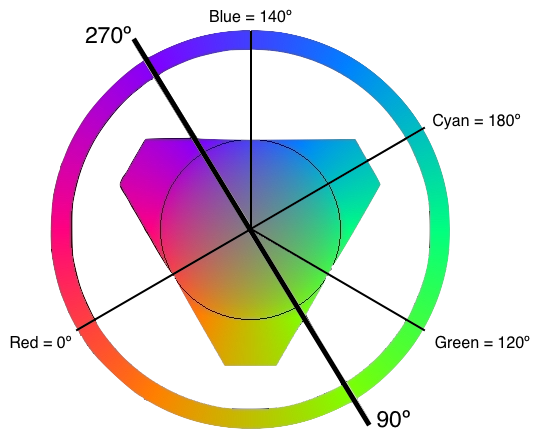
\includegraphics[width=0.25\textwidth]{images/results/HSV_hue.png}
    \caption[Example of HSV Hue Circle, with opposed hue values.]{Example of HSV Hue Circle, with opposed hue values.}
    \label{fig:hsvcircles_example}
\end{wrapfigure}
%
The HSV Color Model, along with CMYK and RGB, is the one which presents the lowest standard deviation of distances between the results from the online environment, which could indicate greater agreement between distances
 to the ideal HSV answer. \par
%
The questions which have shorter distances are number eleven (given orange and expected green and magenta), number seventeen (given green, expected blue and yellow) and number six (given orange,
expected red and yellow), with mean values of $\overline{x} = 0.0587$, $\overline{x} = 0.0683$ and $\overline{x} = 0.0741$, respectively.
On the other hand, we found that the questions which generate the worst results are number two (given magenta, expected red and blue), number thirteen (given a shade of blue, expected blue and cyan) and number
ten (given a shade of blue, expected green and magenta), with correspondent mean values $\overline{x}_{2} = 0.2173$, $\overline{x}_{13} = 0.2713$ and
$\overline{x}_{10} = 0.3$.
By analyzing Table \ref{table:colormodels_distances_labonline_statistics}, we can conclude that the HSV color model is the one which has a wider range of distances (laboratory environment) compared to other models. \par
%
When comparing the results from the HSV color model with other color models' results, we detected some statistically significant differences with other models: performing a Wilcoxon Test ($p < 0.05$), we can infer that HSV does
have statistically significant differences with CIE-L*C*h*, CMYK, RGB and CIE-L*a*b* in the majority of questions. The model which HSV has least statistically significant differences with is RGB, with seven questions. \par
%
As referred before, there are some color blends that, due to the fact that primitives of the mixture are precisely opposed ($180º$) in the HSV hue circle, the blending in HSV Model could produce two different outputs.
This occurs if one mixes the colors obeying to a positive or negative rotation on the circle (as seen on Figure \ref{fig:hsvcircles_example}). There are in this study three pairs of colors which blend onto two possible
colors: pair Red-Cyan (with possible outputs question three and four), pair Green-Magenta (questions ten and eleven) and pair Blue-Yellow (questions fifteen and sixteen). By placing these questions, we intended to
understand which side the user would tend to follow (or even if he follows one) when asked to indicate the blending-basis. The results for each question were already analyzed in the previous subSection, therefore we
present the essence of them in the following topics:
%
\begin{enumerate}
  \item \ul{Red \& Cyan Blend} - Analyzing answers for questions three and four, they produce fairly similar results: they are both a bit far from the reference pair ($\overline{x}_{distance-3} = 0.0941$ and
  $\overline{x}_{HSV-4} = 0.1162$), although the mean distance to the HSV pre-calculated blending for question three has a slightly lower value than question four. This could be also compared to question 12, which also
  produces \textbf{Lime-Green} like question three, but even when compared, question three still has the best results when generating this tone of green. This leads us to specify that, although the mean distances to the
  ideal HSV Color blend for this mixture, are not the lowest among all questions, \textbf{the users show a tendency to associate the blending of red and cyan to a result of lime-green, instead of shade of purple}. When comparing
  these results with online, we found that the later ones corroborate and prove this conclusion.
  %
  \item \ul{Green \& Magenta Blend} - Unlike the previous blend, the results between these questions were quite different between each other concerning the distance to the reference pair: $\overline{x}_{HSV-10} = 0.3$
  and $\overline{x}_{HSV-11} = 0.0587$. However, the lower results associated with question eleven are due to the simple fact that \textbf{users indicated answers pairs which contained Red and Yellow}, which is the pair
  analyzed previously that also blended into orange; if the distance to the ideal answer pair for this question was measured, its mean value would be $\overline{x}_{distanceC1-C2} = 0.645$, which is largely different from the
  reference pair. Therefore we can conclude that \textbf{it is hard for the users to blend green and magenta, to obtain either a blue or an orange shade}; we can also conclude that \textbf{the blending of red and yellow
  onto an orange color, is a strongly implemented color mixture, in mental models of our users}.
  %
  \item \ul{Blue \& Yellow Blend} - Evaluating the results obtained on question fifteen and sixteen, we obtain different results for both. Analyzing results of question fifteen, we know that the distance to the expected
  pair of colors it presents one of the lowest values among all results for HSV Color Model ($\overline{x}_{HSV-15} = 0.09$, $s_{HSV-15} = 0.03559$); however, when comparing the result-pairs given on this question, with
  the ones given on question nine (which presented the exact same shade of green, when asked for pair Green-Cyan), question fifteen still presents the results to generate this color.
  As it can be seen on Figure \ref{fig:labhsvregular_15}, the resulting blend in HSV Color Model tend to be close to the ideal HSV answer: despite being nearer to the top corner of the HSV Model Triangle, \textbf{we can still
  consider the answers to be a tone of green color}. Regarding the results from question 16, they present themselves to be one of the worst for this color model: the distance to the reference pair is $\overline{x}_{HSV-16} = 0.2087$
  and the standard deviation for the distances of answers blended in HSV is $s_{HSV-16} = 0.10378$. Since the presented color had a strong value of red component, users tended their answers to the red shade, while blending
  it with a purple or pink one, to indicate a mixture close to magenta. This indicates that \textbf{blending Blue and Yellow, in HSV Color Model, does not correspond to a red shade, but to a green one, according to
  the users' expectations}.
  %
  \begin{figure}[!htbp]
    \centering
    \begin{minipage}{0.48\textwidth}
      \centering
      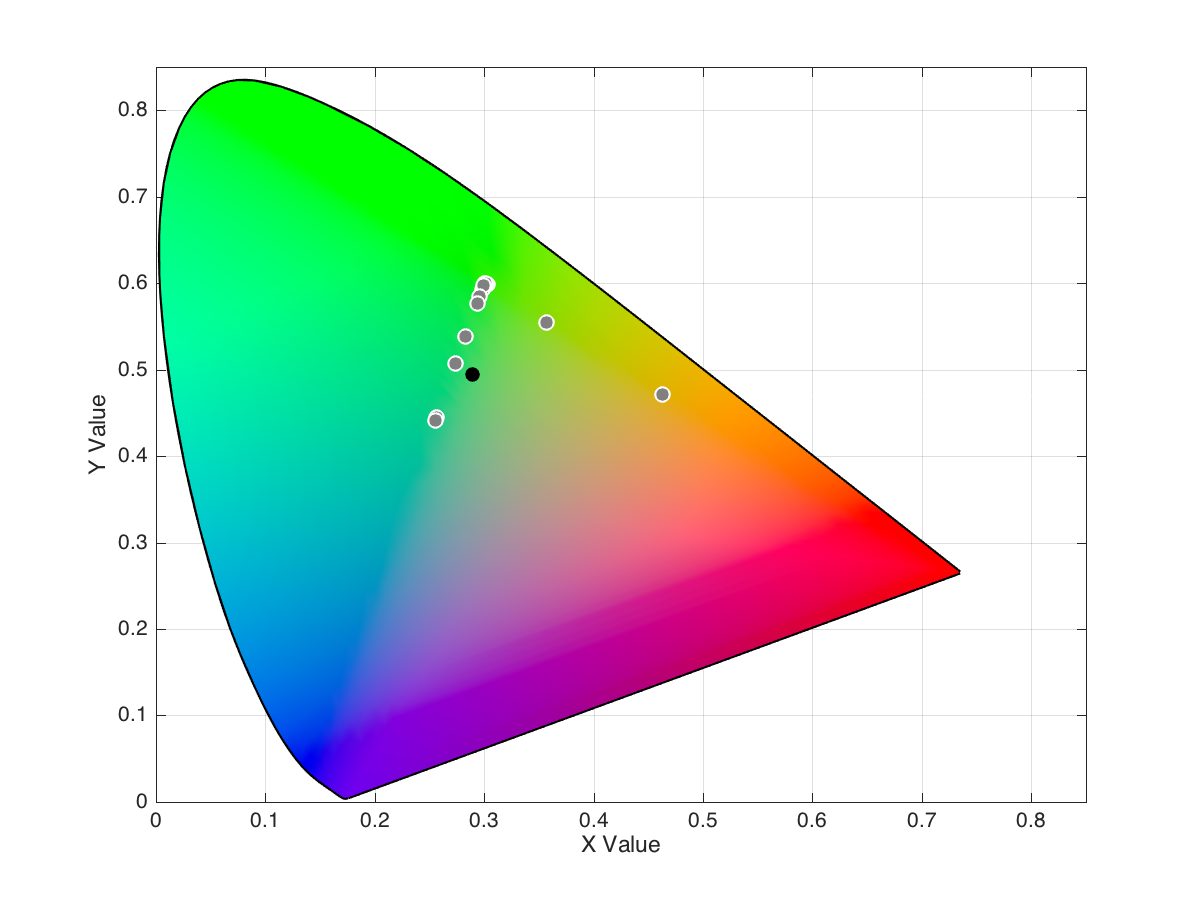
\includegraphics[width=\textwidth]{images/results/15_lab_HSVresponses.png}
      \caption[Laboratory: Answers for Question 15, from regular users, mixed in HSV Color Model.]{Laboratory: Answers for Question 15, from regular users, mixed in HSV Color Model.}
      \label{fig:labhsvregular_15}
    \end{minipage}\hfill
    \begin{minipage}{0.48\textwidth}
      \centering
      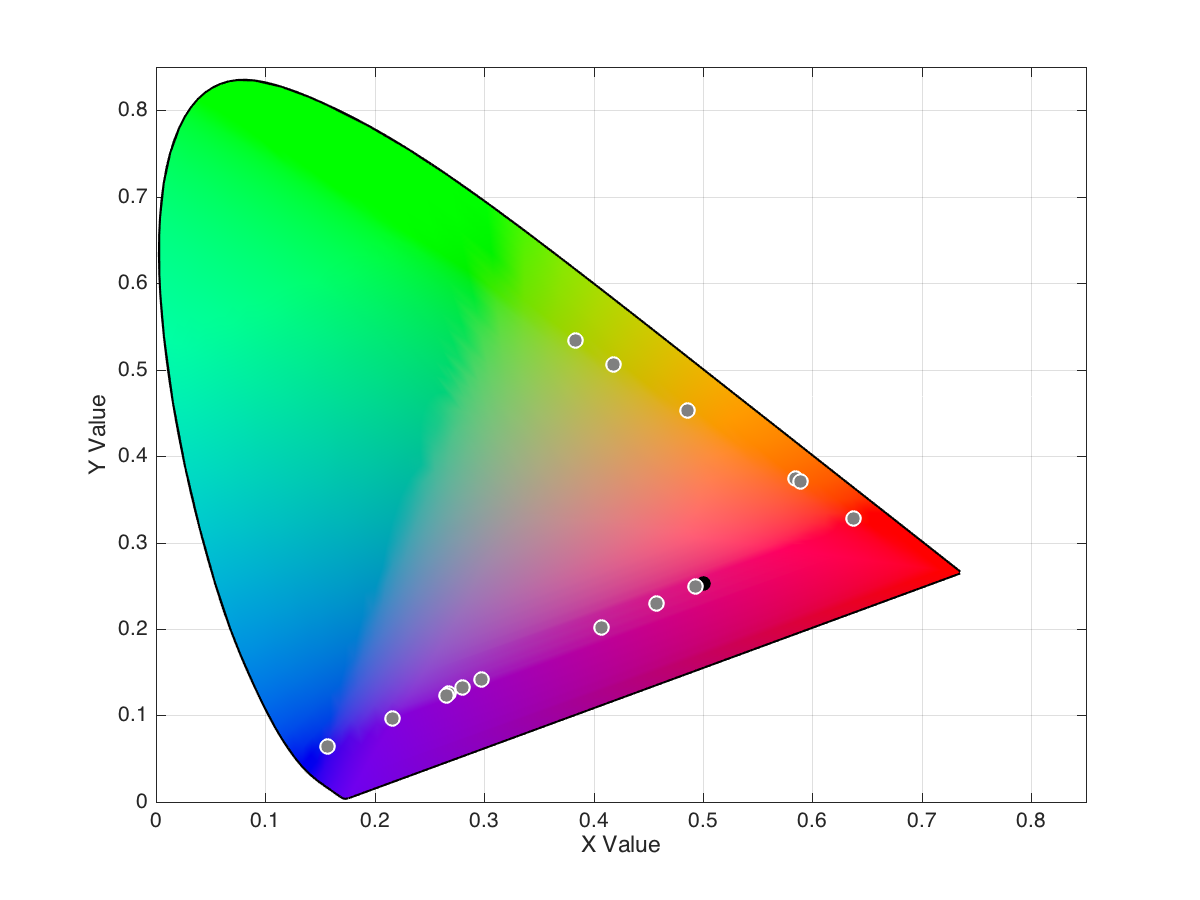
\includegraphics[width=\textwidth]{images/results/16_lab_HSVresponses.png}
      \caption[Laboratory: Answers for Question 16, from regular users, mixed in HSV Color Model.]{Laboratory: Answers for Question 16, from regular users, mixed in HSV Color Model.}
      \label{fig:labhsvregular_16}
    \end{minipage}
    \vspace{-5pt}
  \end{figure}
  %
\end{enumerate} \par
%
Another interesting example are Question 10 and 13: they both present a shade of blue, which could be obtained by two combinations, either Green and Magenta (Question ten) or Blue and Cyan (Question thirteen). Particularly, the
late question had a fairly simple expected pair (two shades of blue), but the users demonstrated some dispersion when answering the question: moreover, the statistics prove it, by having a rather high standard deviation
($\overline{x}_{HSV-10} = 0.3$, $s_{HSV-10} = 0.15792$) when compared to the standard deviation of the whole model ($s_{HSV} = 0.08$). These results are, thus, consistent with the know fact revealed in the Background of this thesis that
\textbf{human color perception is poorer in the blue region of the color spectrum, than in others}, \emph{e.g} the green zone, which produced the best results for this color model; these results are extensible to the purple region
of the spectrum, which is contiguous to the blue one. \par
%
The diagram of Figure \ref{fig:hsv_analysis} contains the three top and bottom-valued questions, disposed on top of an interval $[0 ; 0.5]$ of differences. Each question is mapped according to its mean value for distance to the ideal
HSV Color Model response, while is accompanied by the range of values which compose its answers. \par
%
\begin{figure}[!htbp]
  \centering
  \vspace{-15pt}
  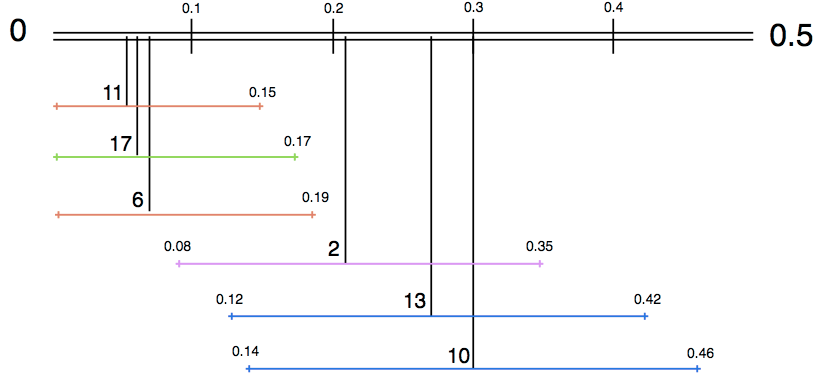
\includegraphics[width=0.65\textwidth]{images/results/hsv_questions_analysis.png}
  \caption[Best and Worst Questions, according to HSV Color Model.]{Best and Worst Questions, according to HSV Color Model.}
  \label{fig:hsv_analysis}
  \vspace{-5pt}
\end{figure}
%
%%%%%%%%%%%%%%%%%% LCh Analise %%%%%%%%%%%%%%%%%%
%
\paragraph{\ul{CIE-L*C*h* Color Model Blendings}} \par
\label{par:lchcolormodel}
%
In turn, the CIE-L*C*h* Color Model is the one which presents the worst results for most of the descriptive statistics present on Table \ref{table:colormodels_distances_labonline_statistics}: it has the highest
mean value on laboratory and online environment, and the highest standard deviation, range and variance exclusively on the online environment. \par
%
The three questions which have shorter distances are number six (given orange, expected red and yellow), number five (given a shade of red, expected red and magenta) and number two (given magenta, expected red
and blue). The mean values distances for this questions were $\overline{x}_{6} = 0.1332$, $\overline{x}_{5} = 0.15$ and $\overline{x}_{2} = 0.1573$ which, contrary to the previous color model, are all values above $0.1$ (a quite
high value in the scale which results are presented), that could represent a significant change in the resultant color. \par
%
On the other hand, we consider that the questions which generate the worst results are number ten (given a shade of blue, expected green and magenta), number fourteen (given a shade of purple, expected blue and magenta) and number
fifteen (given a shade of green, expected blue and yellow), with correspondent mean values $\overline{x}_{10} = 0.2557$, $\overline{x}_{14} = 0.2995$ and $\overline{x}_{15} = 0.3031$. Curiously, the standard deviations of distances (for the
laboratory environment) in this color model are fairly low when compared to the previous color model. \par
%
When comparing the results from the CIE-L*C*h* color model with other color models' results, we detect some statistically significant differences with other models: performing a Wilcoxon Test ($p < 0.05$), we can infer that CIE-L*C*h* does
present statistically significant differences with HSV, CMYK, RGB and CIE-L*a*b* in the majority of questions (between 8 to 10 questions). The model which CIE-L*C*h* has most statistically significant differences with is CMYK, with eleven questions. \par
%
Question six presented again a constant top value for the mean value, on this model, which reinforces the theory that the \textbf{orange color is commonly used and mixed by the users}. On the other hand, question number
ten kept having one of the worst mean ($\overline{x}_{10} = 0.2557$) and deviation ($s_{10} = 0.1164$) values, strengthening the theory that \textbf{blue shades and tones will probably wild worst results, due to the fact
that it is the color which human have less descriptive power}. \par
%
\begin{figure}[!htbp]
  \centering
  \vspace{-15pt}
  \begin{minipage}{0.48\textwidth}
    \centering
    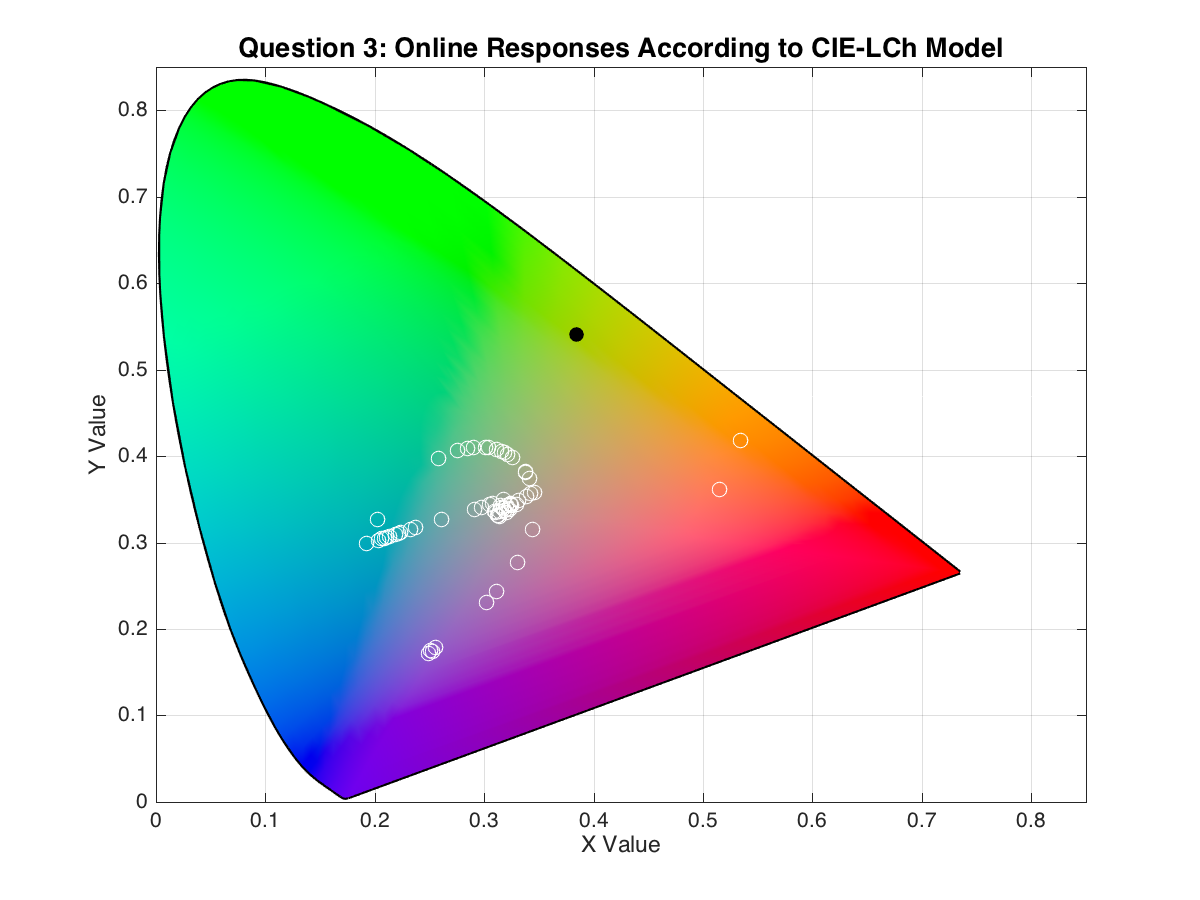
\includegraphics[width=\textwidth]{images/results/3_online_LChresponses.png}
    \caption[Online: Answers for Question 3, from regular users, mixed in CIE-L*C*h* Color Model.]{Online: Answers for Question 3, from regular users, mixed in CIE-L*C*h* Color Model.}
    \label{fig:onlinelchregular_3}
  \end{minipage}\hfill
  \begin{minipage}{0.48\textwidth}
    \centering
    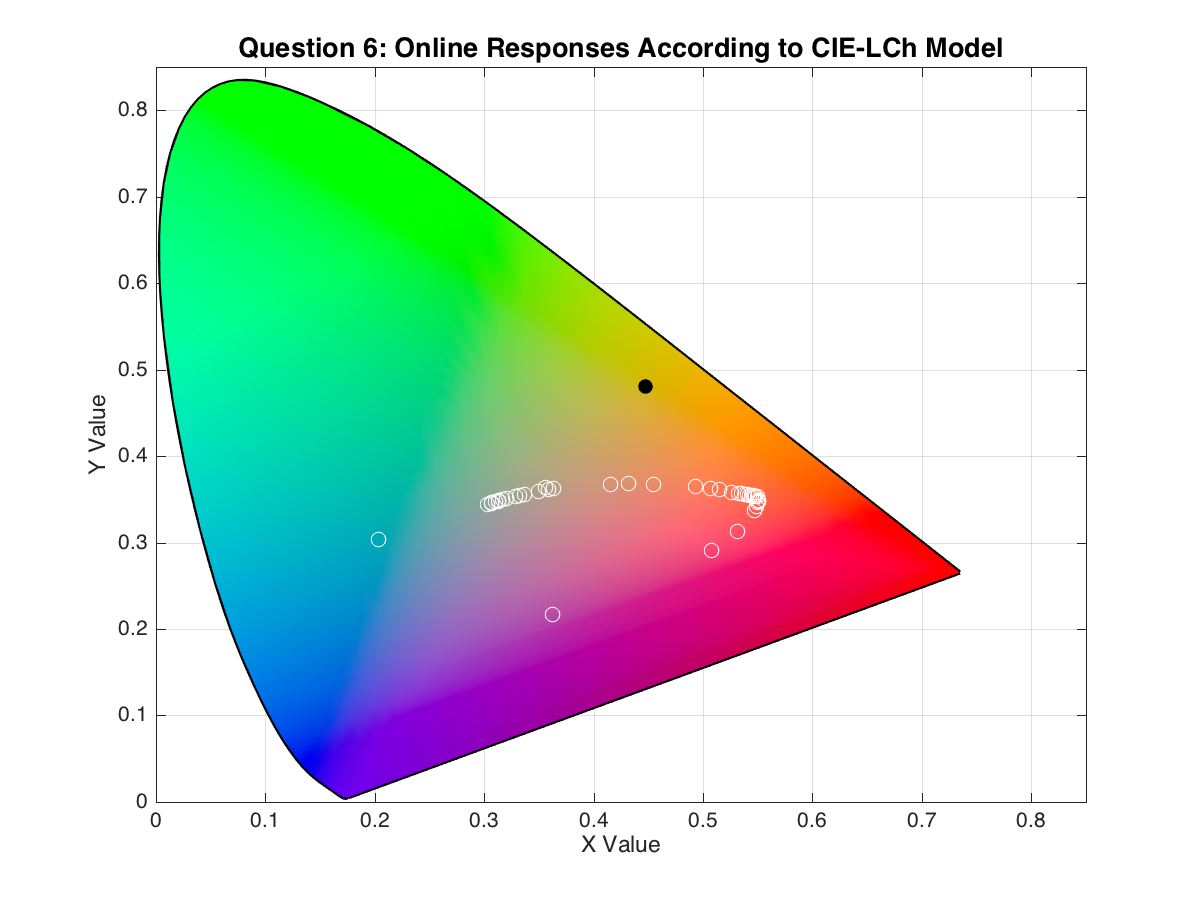
\includegraphics[width=\textwidth]{images/results/6_online_LChresponses.png}
    \caption[Online: Answers for Question 6, from regular users, mixed in CIE-L*C*h* Color Model.]{Online: Answers for Question 6, from regular users, mixed in CIE-L*C*h* Color Model.}
    \label{fig:onlinelchregular_6}
  \end{minipage}
  \vspace{-5pt}
\end{figure}
%
The question which revealed one of the lowest standard deviation value (meaning less oscillation of results), relating the online environment, was question three ($s_{3} = 0.05855$): this question help us
illustrate the difference between each of the descriptive statistics, since it has one of the highest mean value of distances ($\overline{x}_{17} = 0.23$) and, at the same time, lowest standard deviation. This could
portray a scenario in which the users agreed on a quite distant answer. This question is illustrated in Figure \ref{fig:onlinelchregular_3}. \par
%
The question which has the lowest mean value of distances was question six ($s_{LCh-6} = 0.1332$), and it is represented on Figure \ref{fig:onlinelchregular_6}. Nonetheless, we can observe that \textbf{these
questions have all answers pairs which, when blended according to CIE-L*C*h*, generate results that are farther apart from the ideal answer of each question}, therefore concluding that \textbf{CIE-L*C*h* is not
the color model which hatches the best results when blending colors, according to users' expectations}. \par
%
The diagram of Figure \ref{fig:lch_analysis} contains the three top and bottom-valued questions, disposed on top of an interval $[0 ; 0.5]$ of differences. Each question is mapped according to its mean value for
distance to the ideal CIE-L*C*h* Color Model response, while is accompanied by the range its answers. \par
%
\begin{figure}[!htbp]
  \centering
  \vspace{-15pt}
  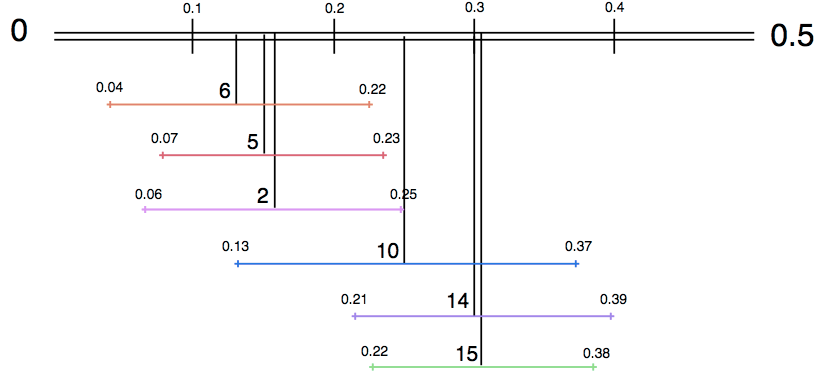
\includegraphics[width=0.65\textwidth]{images/results/lch_questions_analysis.png}
  \caption[Best and Worst Questions, according to CIE-L*C*h* Color Model.]{Best and Worst Questions, according to CIE-L*C*h* Color Model.}
  \vspace{-5pt}
  \label{fig:lch_analysis}
\end{figure}
%
%%%%%%%%%%%%%%%%%% CMYK Analise %%%%%%%%%%%%%%%%%%
%
\paragraph{\ul{CMYK Color Model Blendings}}
\label{par:cmykcolormodel}
%
The CMYK Color Model is, by far, the one which presents the best results for most of the descriptive statistics present on Table \ref{table:colormodels_distances_labonline_statistics}: it has the lowest mean value of distances ($\overline{x}_{lab} = 0.10$, $\overline{x}_{online} = 0.09$), lowest standard deviation ($s_{lab} = 0.04$, $s_{online} = 0.04$),
the lowest range of values ($range_{lab} = 0.14$, $range_{online} = 0.11$) and, finally, the lowest variance value ($s^2_{lab} = 0.001$, $s^2_{online} = 0.001$). \par
%
The three questions which have shorter distances are number seventeen (given a green, expected cyan and blue), number six (given orange, expected red and yellow) and number fifteen (given a shade of green, expected blue
and yellow). The mean values distances for this questions were $\overline{x}_{17} = 0.0452$, $\overline{x}_{6} = 0.0577$ and $\overline{x}_{15} = 0.0625$ which, contrary to the previous color model, are all values \ul{below $0.1$},
that does not represent a significant change in the resultant color. \par
%
On the other hand, we consider that the questions which generate the worst results are number ten (given a shade of blue, expected green and magenta) and twelve (given a tone of green, expected green and yellow), number five
(given a shade of red, expected red and magenta) and number thirteen (given a shade of blue, expected blue and cyan), with correspondent mean values $\overline{x}_{10-12} = 0.1314$, $\overline{x}_{5} = 0.1322$ and
$\overline{x}_{13} = 0.1875$. Comparing them with the CIE-L*C*h* Color Model, we can easily observe that these values are very low when compared with the later's worst results. \par
%
Question six keeps presenting a constant top value for the mean value, on this model, while question number ten and thirteen (both presented blue shades) kept having the worst mean and deviation values ($\overline{x}_{13} = 0.1875$,
$s_{13} = 0.13097$), strengthening the theories aforementioned. \par
%
When comparing the results from the CMYK color model with other color models' results, we detect some statistically significant differences with other models: performing a Wilcoxon Test ($p < 0.05$), we can infer that CMYK does
present statistically significant differences with HSV, CIE-L*C*h*, RGB and CIE-L*a*b* in the majority of questions. The model which CMYK has most statistically significant differences with is RGB, with thirteen questions. \par
%
Question seventeen presented consistently another low value: along with question three and fifteen, these presented different \ul{shades of green} and all had yielded favorable results. Having this in mind, this may lead us to
form another conclusion: \textbf{questions which presented shades of green color may produce better results, according to users' expectations}. This is consistent with the fact that \textbf{humans have more descriptive power
in the green zone of the spectrum, due to the amount of cones which exist in the human eye}. \par
%
As it was explained before in the theoretical background, this color model is mainly a subtractive one, meaning it will naturally darken the colors when they are blended; the questions which yielded \textbf{better results are majorly
related to primitives of the CMYK color model}. This success could be related to the fact that \textbf{people tend to formulate mental models of color based on ink mixing in childhood} \cite{Gossett2004}, mostly associating it to
RYB and CMYK Color Models without even knowing it. \par
%
\begin{figure}[!htbp]
  \centering
  \vspace{-5pt}
  \begin{minipage}{0.48\textwidth}
    \centering
    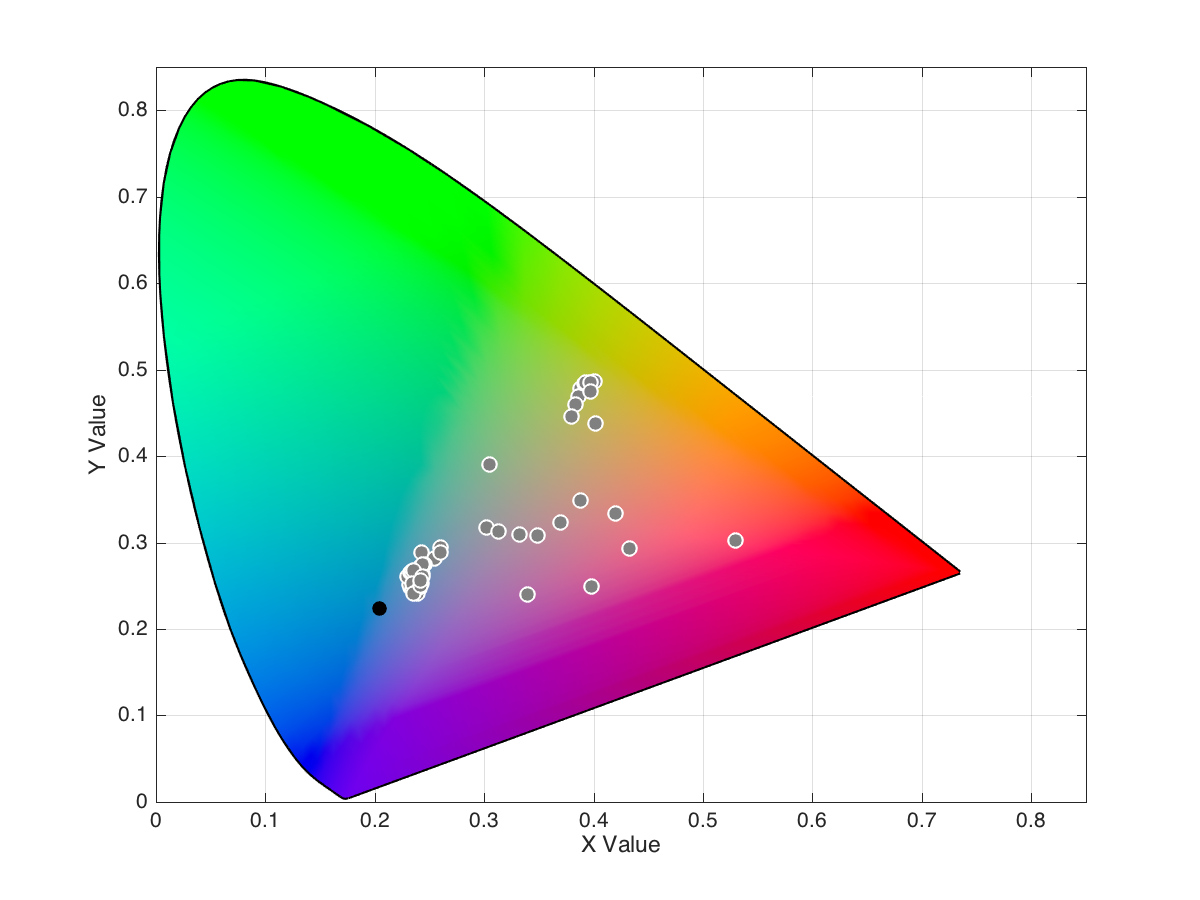
\includegraphics[width=\textwidth]{images/results/13_online_CMYKresponses.png}
    \caption[Online: Answers for Question 13, from regular users, mixed in CMYK Color Model.]{Online: Answers for Question 13, from regular users, mixed in CMYK Color Model.}
    \label{fig:onlinecmykregular_13}
  \end{minipage}\hfill
  \begin{minipage}{0.48\textwidth}
    \centering
    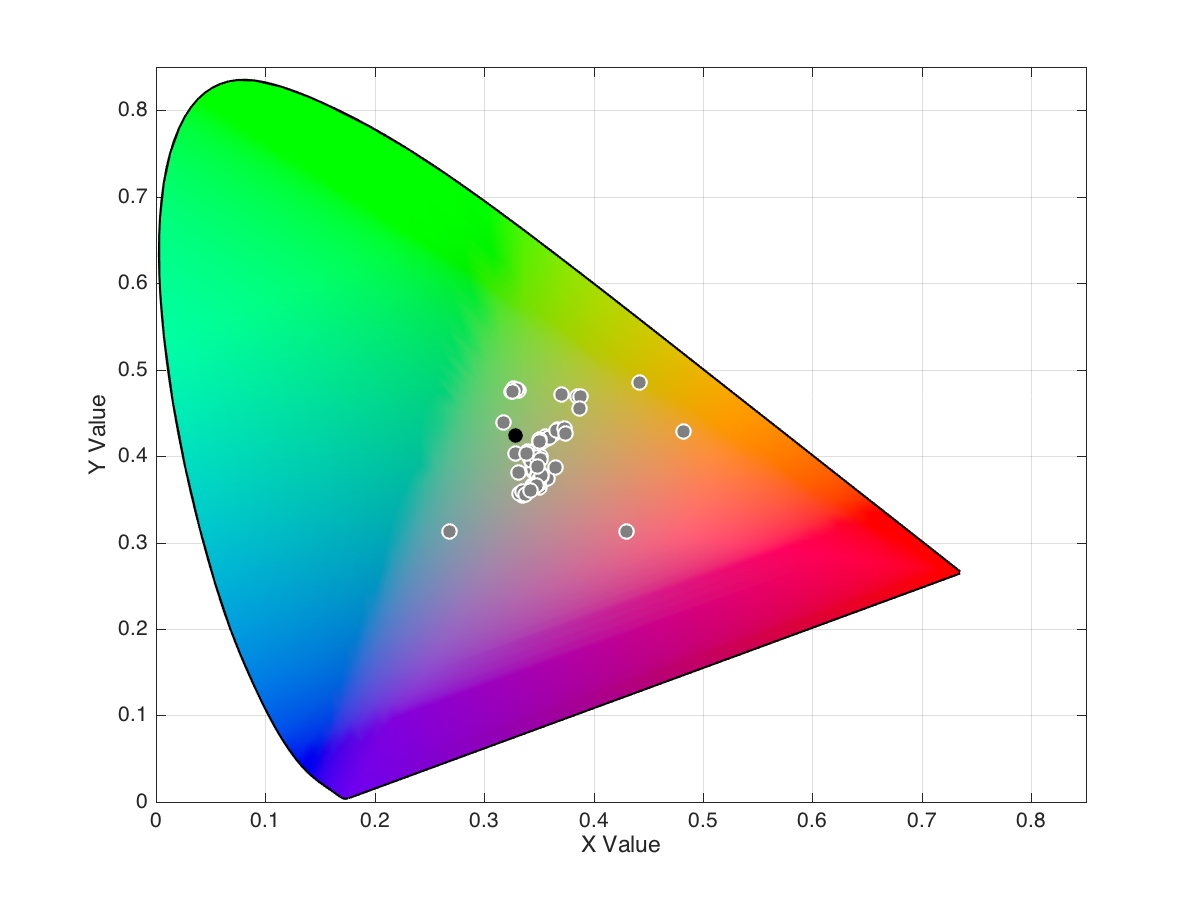
\includegraphics[width=\textwidth]{images/results/17_online_CMYKresponses.png}
    \caption[Online: Answers for Question 17, from regular users, mixed in CMYK Color Model.]{Online: Answers for Question 17, from regular users, mixed in CMYK Color Model.}
    \label{fig:onlinecmykregular_17}
  \end{minipage}
  \vspace{-5pt}
\end{figure}
%
These results indicate that \textbf{CMYK is a highly compatible color model with the users expectations}, as this model presents statistics which prove that CMYK had smaller distances to ideal answers and lower deviation of answers.
Figure \ref{fig:onlinecmykregular_13} represents the results of Question 13, which had wider distances to the pre-calculated CMYK blend, and Figure \ref{fig:onlinecmykregular_17} show the results for Question 17, the question with closer
distances. The diagram of Figure \ref{fig:cmyk_analysis} contains the three top and bottom-valued questions, disposed on top of an interval $[0 ; 0.5]$ of differences. Each question is mapped according to its mean value for
distance to the ideal CMYK Color Model response, while is accompanied by the range of values which compose its answers. \par
%
\begin{figure}[!htbp]
  \centering
  \vspace{-15pt}
  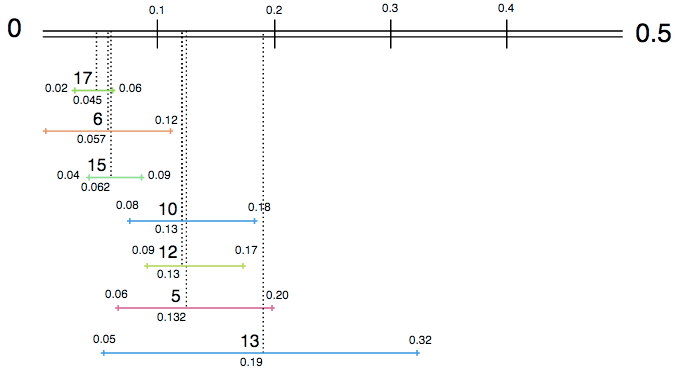
\includegraphics[width=0.65\textwidth]{images/results/cmyk_questions_analysis.png}
  \caption[Best and Worst Questions, according to CMYK Color Model.]{Best and Worst Questions, according to CMYK Color Model.}
  \vspace{-5pt}
  \label{fig:cmyk_analysis}
\end{figure}
%
%%%%%%%%%%%%%%%%%% RGB Analise %%%%%%%%%%%%%%%%%%
%
\paragraph{\ul{RGB Color Model Blendings}}
\label{subsubsec:rgbcolormodel}
%
This color model, as covered before, is complementary to the CMYK color model. Feedback collected from the users was such that, sometimes, the users which knew how to blend in subtractive color models,
tended to be confused and tried to mix additive color models, also. Based on the results collected from the laboratory users, we can tell that the results from this color model are quite similar to CMYK results: the descriptive statistics present
on Table \ref{table:colormodels_distances_labonline_statistics}, prove RGB has one of the lowest mean value of distances ($\overline{x}_{lab} = 0.14$, $\overline{x}_{online} = 0.12$) and one of
the lowest standard deviations ($s_{lab} = 0.05$, $s_{online} = 0.04$ equal to $s_{CMYK-online}$). \par
%
The three questions which have shorter distances are number number six (given orange, expected red and yellow), number nine (given a shade of green, expected green and cyan) and seventeen (given a green, expected cyan and blue). The mean values
distances for this questions were $\overline{x}_{6} = 0.0777$, $\overline{x}_{9} = 0.1005$ and $\overline{x}_{17} = 0.1030$.
On its turn, we consider that the questions which generate the worst results are number two (given magenta, expected red and blue), number ten (given a shade of blue, expected green and magenta) and, again, number thirteen (given a shade of blue,
expected blue and cyan), with correspondent mean values $\overline{x}_{2} = 0.1660$, $\overline{x}_{10} = 0.2107$ and $\overline{x}_{13} = 0.2450$.
Comparing them with the CIE-L*C*h* Color Model, we can observe these values are likely to be similar when compared with the later's worst results, but a little high when compared with CMYK results. \textbf{The colors orange and green continue to
present the best values, while the blue shades are the lowest}. \par
%
\begin{figure}[!htbp]
  \centering
  \vspace{-15pt}
  \begin{minipage}{0.48\textwidth}
    \centering
    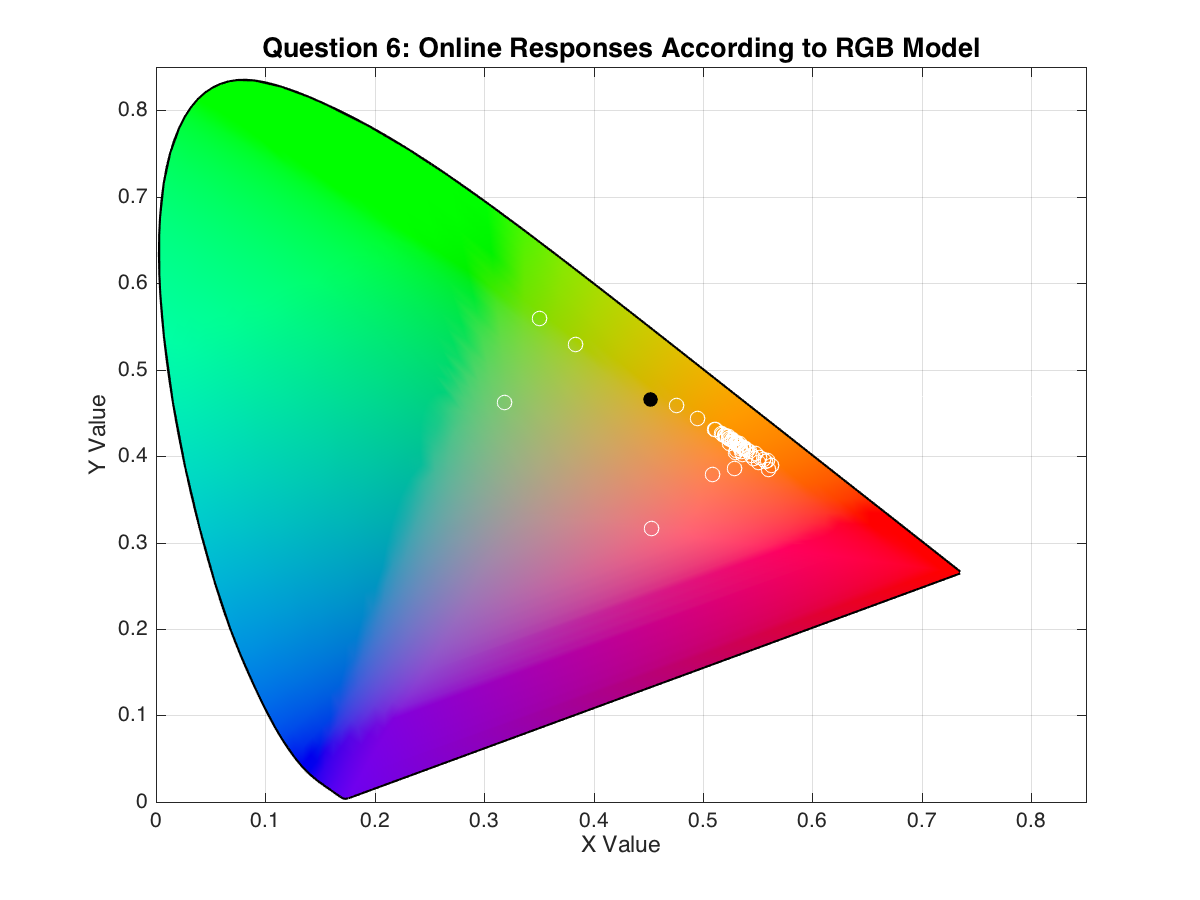
\includegraphics[width=\textwidth]{images/results/6_online_RGBresponses.png}
    \caption[Online: Answers for Question 6, from regular users, mixed in RGB Color Model.]{Online: Answers for Question 6, from regular users, mixed in RGB Color Model.}
    \label{fig:onlinergbregular_6}
  \end{minipage}\hfill
  \begin{minipage}{0.48\textwidth}
    \centering
    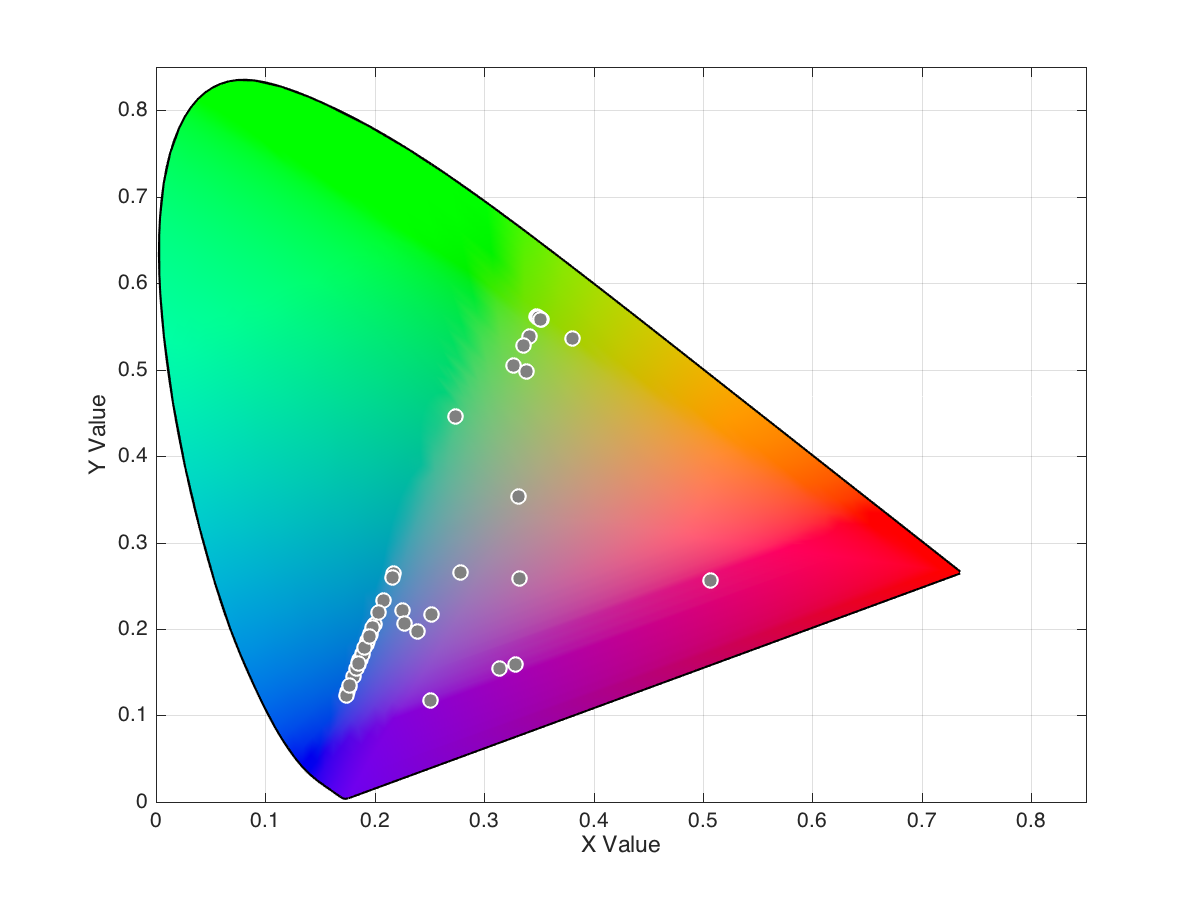
\includegraphics[width=\textwidth]{images/results/13_online_RGBresponses.png}
    \caption[Online: Answers for Question 13, from regular users, mixed in RGB Color Model.]{Online: Answers for Question 13, from regular users, mixed in RGB Color Model.}
    \label{fig:onlinergbregular_13}
  \end{minipage}
  \vspace{-5pt}
\end{figure}
%
When comparing the results from the RGB color model, the majority of users did reveal lack of knowledge in mixing the colors according to an additive color model, as they tended to mix colors according to the CMYK color model. However, this color
model has a high degree of compatibility with every other model, excepting CMYK: performing a Wilcoxon Test ($p < 0.05$), we can infer that RGB does not present statistically significant differences with HSV, CIE-L*a*b* and with CIE-L*C*h* in 10
questions, while presenting statistically significant differences with CMYK in 13 questions.
Relating to the fact that people either tend to blend colors in an additive or subtractive way, we can compare the results from this color model with CMYK model and state that \textbf{users tend to formulate subtractive mental models of color
blending}. However, \textbf{there is room for further investigation, to fully understand if users are influenced by additive color models or subtractive ones}. \par
%
Figure \ref{fig:onlinergbregular_6} represents the results of Question 6, which had the shortest distances to the pre-calculated RGB blend, and Figure \ref{fig:onlinergbregular_13} show the results for Question 13, the question with wider
distances. The diagram of Figure \ref{fig:rgb_analysis} contains the three top and bottom-valued questions, disposed on top of an interval $[0 ; 0.5]$ of differences. \par
%
\begin{figure}[!htbp]
  \centering
  \vspace{-15pt}
  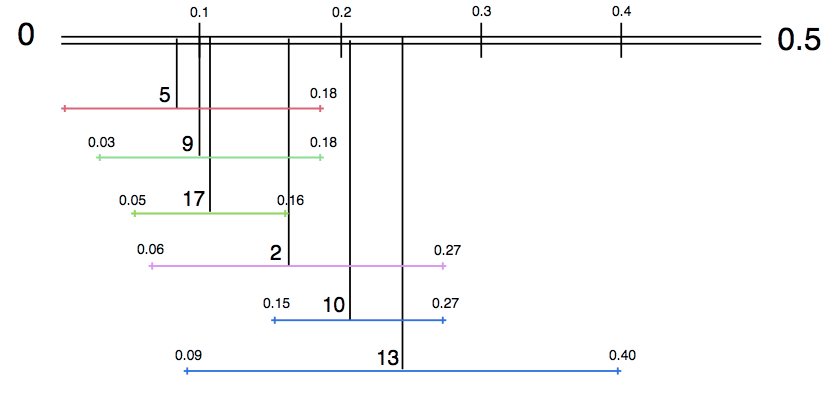
\includegraphics[width=0.65\textwidth]{images/results/rgb_questions_analysis.png}
  \caption[Best and Worst Questions, according RGB Color Model.]{Best and Worst Questions, according to RGB Color Model.}
  \vspace{-5pt}
  \label{fig:rgb_analysis}
\end{figure}
%
%%%%%%%%%%%%%%%%%% Lab Analise %%%%%%%%%%%%%%%%%%
%
\paragraph{\ul{CIE-L*a*b* Color Model Blendings}} \par
\label{par:labcolormodel}
%
This color model has results very similar to CMYK and RGB, since its descriptive statistics have comparable values to this model.
The three questions which have shorter distances are number number six (given orange, expected red and yellow), seventeen (given a green, expected cyan and blue) and number nine (given a shade
of green, expected green and cyan), which are exactly the same as before. The mean values distances for this questions were $\overline{x}_{6} = 0.0509$, $\overline{x}_{17} = 0.1130$ and $\overline{x}_{9} = 0.1142$. \par
%
\begin{figure}[!htbp]
  \centering
  \vspace{-15pt}
  \begin{minipage}{0.48\textwidth}
    \centering
    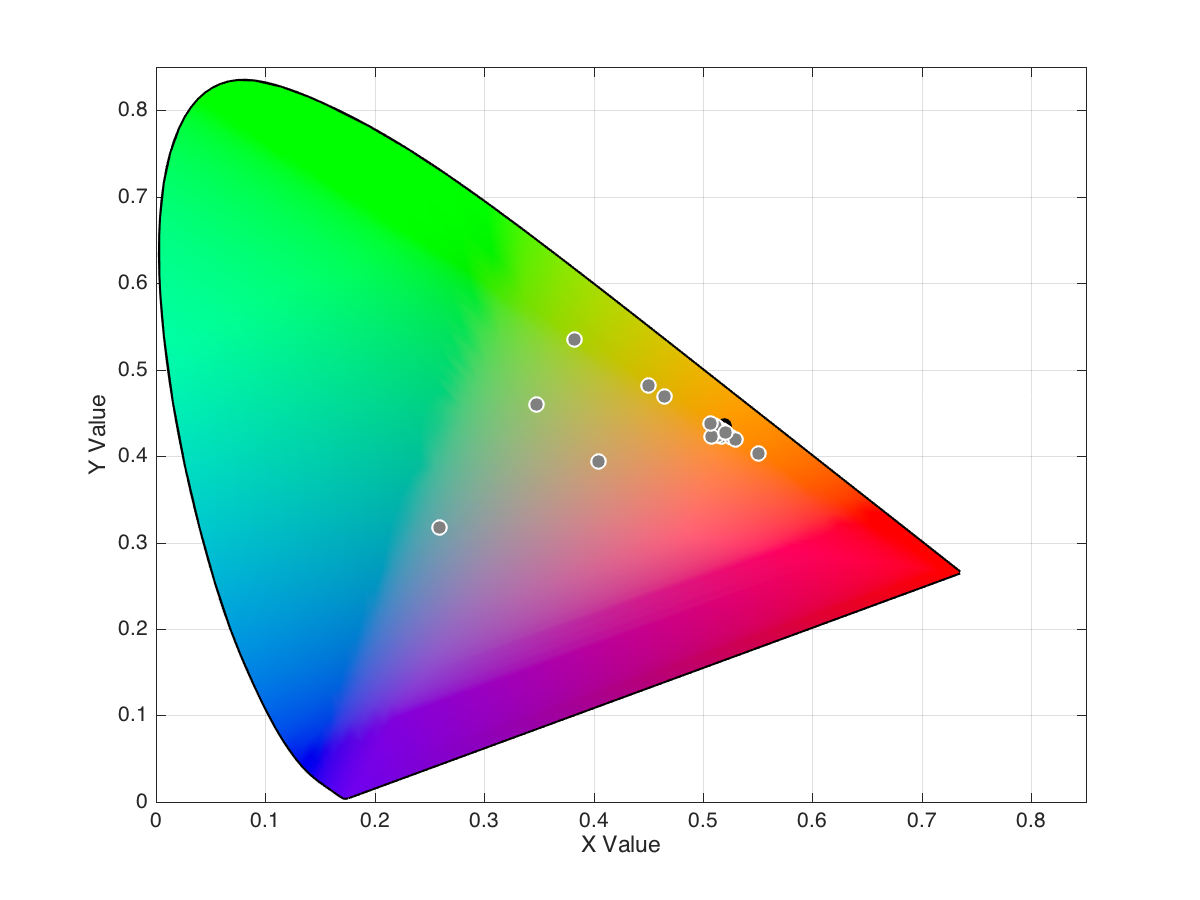
\includegraphics[width=\textwidth]{images/results/6_lab_Labresponses.png}
    \caption[Laboratory: Answers for Question 6, from regular users, mixed in CIE-L*a*b* Color Model.]{Laboratory: Answers for Question 6, from regular users, mixed in CIE-L*a*b* Color Model.}
    \label{fig:lablabregular_6}
  \end{minipage}\hfill
  \begin{minipage}{0.48\textwidth}
    \centering
    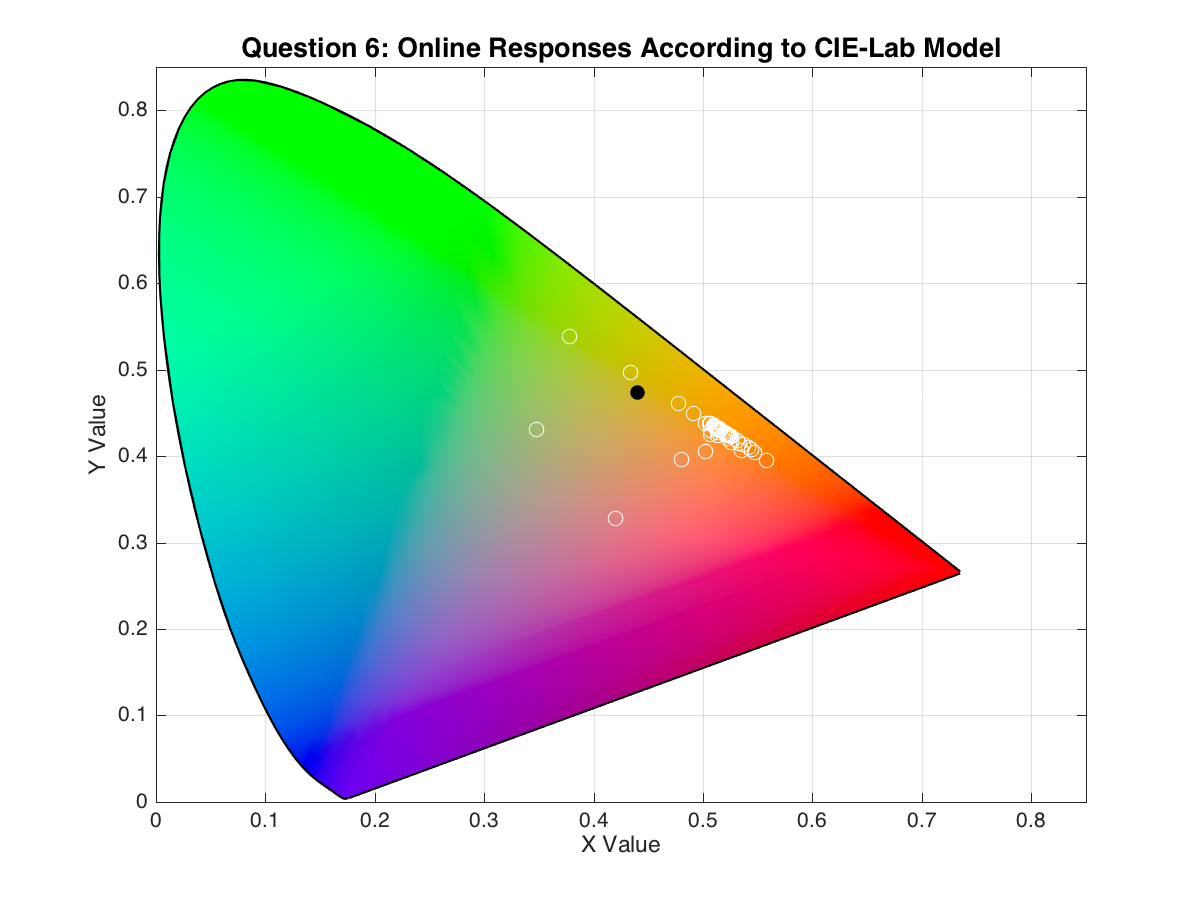
\includegraphics[width=\textwidth]{images/results/6_online_Labresponses.png}
    \caption[Online: Answers for Question 6, from regular users, mixed in CIE-L*a*b* Color Model.]{Online: Answers for Question 6, from regular users, mixed in CIE-L*a*b* Color Model.}
    \label{fig:onlinelabregular_6}
  \end{minipage}
  \vspace{-5pt}
\end{figure}
%
Considering the questions which generate the worst results are number twelve (given a tone of green, expected green and yellow), number ten (given a shade of blue, expected green and magenta) and number thirteen
(given a shade of blue, expected blue and cyan), with correspondent mean values $\overline{x}_{12} = 0.1743$, $\overline{x}_{10} = 0.2107$ and $\overline{x}_{13} = 0.2450$. Comparing them with the CIE-L*C*h* Color Model
(which is currently the worst-valued color model), we can check that these values are (similar to RGB and HSV) nearer to the later's worst results, but still high when compared with CMYK results (so far, the
best-valued color model). \textbf{The colors orange and green proved, once again, that they are capable of producing the best values, while the blue shades provided the lowest again}. \par
%
When comparing the results from the CIE-L*a*b* color model, we detected that this model has significant differences with all other color models: performing a Wilcoxon Test ($p < 0.05$), we can infer that
CIE-L*a*b* does present statistically significant differences with HSV, CMYK and with CIE-L*C*h* in only nine questions, while presenting no statistically significant differences with RGB
in ten questions.
Since the CIE-L*a*b* conveys the entire set of perceived by the human eye, it \textbf{explains why the results associated with this color model are so close to others which yield the best results}.
Figure \ref{fig:lablabregular_6} represents the laboratory results of Question 6, which not only had the best mean value to the pre-calculated RGB blend, but also its best mean value across all color models,
and Figure \ref{fig:onlinelabregular_6} shows the results for the same question, but the online results which confirm the laboratory ones. The diagram of Figure \ref{fig:lab_analysis} contains the three top and bottom-valued questions, disposed on top of an interval $[0 ; 0.5]$ of differences. \par
%
\begin{figure}[!htbp]
  \centering
  \vspace{-15pt}
  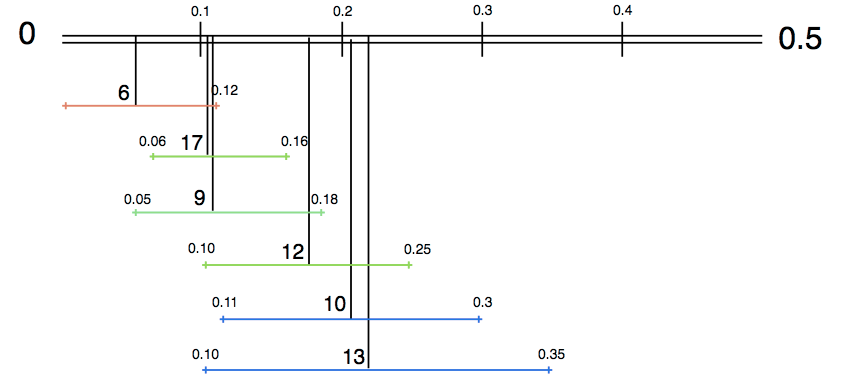
\includegraphics[width=0.65\textwidth]{images/results/lab_questions_analysis.png}
  \caption[Best and Worst Questions, according to CIE-L*a*b* Color Model.]{Best and Worst Questions, according to CIE-L*a*b* Color Model.}
  \vspace{-5pt}
  \label{fig:lab_analysis}
\end{figure}
%
\subsubsection{Color Blending Expectation}
\label{subsubsec:colorblending_exp}
%
Besides asking our users to indicate us the two primitives which composed a color blending of two colors, we intended to go further: \textbf{comprehend if more than detecting two colors of a mixture, a user
is capable of mentally blend two given colors and indicate us its results}. \par
%
Therefore, we reverted the previously analyzed seventeen questions, giving the two primitives of the blending to the user, offering at the same time a color slider which contained discretized pre-calculated
values (which were nothing more than all the results of all questions, blended accordingly to all color models). Contrary to what was done previously, \textbf{we did not blend the answer given by the user,
since the colors presented were already blended}, missing only to calculate the distance of answers to the ideal ones: the results for these questions are expressed on Table \ref{table:expectation_distances_labonline},
with cells shaded in green which represent the best value for each one of questions. \par
%
\begin{table}[!htbp]
  \centering
  \resizebox{0.8\textwidth}{!} {
  \begin{tabular}{@{}cccccclccccclcccc@{}}
    \toprule
                                     & \multicolumn{2}{c}{Presented Colors}                        & \multicolumn{2}{c}{}                                                                                                  & \multicolumn{6}{c}{Laboratory Environment}                                                                                                                                                                                                                                                                     & \multicolumn{6}{c}{Online Environment}                                                                                                                                                                                                                                                                         \\ \cmidrule(lr){2-3} \cmidrule(l){6-17}
    \multirow{-2}{*}{Question ID}    & C1                           & C2                           & \multicolumn{2}{c}{\multirow{-2}{*}{Reference Pair}}                                                                  & \multicolumn{2}{c}{HSV}                                    & CIE-L*C*h*                                                 & CMYK                                                       & RGB                                                        & CIE-L*a*b*                                                 & \multicolumn{2}{c}{HSV}                                    & CIE-L*C*h*                                                 & CMYK                                                       & RGB                                                        & CIE-L*a*b*                                                 \\ \midrule
    \multicolumn{1}{c|}{Question 18} & \multicolumn{1}{c|}{Red}     & \multicolumn{1}{c|}{Green}   & \multicolumn{2}{c||}{\cellcolor[HTML]{FFFF00}(77, 93, 14)}                                                             & \multicolumn{2}{c|}{0.14}                                  & \multicolumn{1}{c|}{0.14}                                  & \multicolumn{1}{c|}{\cellcolor[HTML]{32CB00}\textbf{0.11}} & \multicolumn{1}{c|}{0.15}                                  & \multicolumn{1}{c||}{0.14}                                  & \multicolumn{2}{c|}{\cellcolor[HTML]{FFFFFF}0.12}          & \multicolumn{1}{c|}{\cellcolor[HTML]{FFFFFF}0.12}          & \multicolumn{1}{c|}{\cellcolor[HTML]{32CB00}\textbf{0.08}} & \multicolumn{1}{c|}{\cellcolor[HTML]{FFFFFF}0.12}          & \multicolumn{1}{c|}{0.11}                                  \\ \midrule
    \multicolumn{1}{c|}{Question 19} & \multicolumn{1}{c|}{Red}     & \multicolumn{1}{c|}{Blue}    & \multicolumn{2}{c||}{\cellcolor[HTML]{FF00FF}(59, 28, 97)}                                                             & \multicolumn{2}{c|}{\cellcolor[HTML]{32CB00}\textbf{0.16}} & \multicolumn{1}{c|}{0.23}                                  & \multicolumn{1}{c|}{0.17}                                  & \multicolumn{1}{c|}{\cellcolor[HTML]{32CB00}\textbf{0.16}} & \multicolumn{1}{c||}{0.19}                                  & \multicolumn{2}{c|}{\cellcolor[HTML]{32CB00}\textbf{0.13}} & \multicolumn{1}{c|}{0.24}                                  & \multicolumn{1}{c|}{0.19}                                  & \multicolumn{1}{c|}{0.14}                                  & \multicolumn{1}{c|}{0.19}                                  \\ \midrule
    \multicolumn{1}{c|}{Question 20} & \multicolumn{1}{c|}{Green}   & \multicolumn{1}{c|}{Blue}    & \multicolumn{2}{c||}{\cellcolor[HTML]{00FFFF}(54, 79, 107)}                                                            & \multicolumn{2}{c|}{0.13}                                  & \multicolumn{1}{c|}{0.17}                                  & \multicolumn{1}{c|}{0.14}                                  & \multicolumn{1}{c|}{0.13}                                  & \multicolumn{1}{c||}{\cellcolor[HTML]{32CB00}\textbf{0.11}} & \multicolumn{2}{c|}{0.12}                                  & \multicolumn{1}{c|}{0.17}                                  & \multicolumn{1}{c|}{0.13}                                  & \multicolumn{1}{c|}{0.12}                                  & \multicolumn{1}{c|}{\cellcolor[HTML]{32CB00}\textbf{0.10}} \\ \midrule
    \multicolumn{1}{c|}{Question 21} & \multicolumn{1}{c|}{Red}     & \multicolumn{1}{c|}{Cyan}    & \multicolumn{1}{c||}{\cellcolor[HTML]{80FF00}(45, 76, 12)} & \multicolumn{1}{c||}{\cellcolor[HTML]{7F00FF}(27, 12, 95)} & \multicolumn{1}{c|}{0.28}    & \multicolumn{1}{l|}{0.23}   & \multicolumn{1}{c|}{0.26}                                  & \multicolumn{1}{c|}{0.13}                                  & \multicolumn{1}{c|}{\cellcolor[HTML]{32CB00}\textbf{0.12}} & \multicolumn{1}{c||}{0.17}                                  & \multicolumn{1}{c|}{0.29}    & \multicolumn{1}{l|}{0.23}   & \multicolumn{1}{c|}{0.26}                                  & \multicolumn{1}{c|}{0.13}                                  & \multicolumn{1}{c|}{\cellcolor[HTML]{32CB00}\textbf{0.12}} & \multicolumn{1}{c|}{0.16}                                  \\ \midrule
    \multicolumn{1}{c|}{Question 22} & \multicolumn{1}{c|}{Red}     & \multicolumn{1}{c|}{Magenta} & \multicolumn{2}{c||}{\cellcolor[HTML]{FF0080}(45, 23, 22)}                                                             & \multicolumn{2}{c|}{\cellcolor[HTML]{32CB00}\textbf{0.18}} & \multicolumn{1}{c|}{0.20}                                  & \multicolumn{1}{c|}{0.25}                                  & \multicolumn{1}{c|}{0.21}                                  & \multicolumn{1}{c||}{0.20}                                  & \multicolumn{2}{c|}{\cellcolor[HTML]{32CB00}\textbf{0.14}} & \multicolumn{1}{c|}{0.16}                                  & \multicolumn{1}{c|}{0.20}                                  & \multicolumn{1}{c|}{0.17}                                  & \multicolumn{1}{c|}{0.16}                                  \\ \midrule
    \multicolumn{1}{c|}{Question 23} & \multicolumn{1}{c|}{Red}     & \multicolumn{1}{c|}{Yellow}  & \multicolumn{2}{c||}{\cellcolor[HTML]{FF8000}(49, 37, 5)}                                                              & \multicolumn{2}{c|}{\cellcolor[HTML]{32CB00}\textbf{0.16}} & \multicolumn{1}{c|}{\cellcolor[HTML]{32CB00}\textbf{0.16}} & \multicolumn{1}{c|}{\cellcolor[HTML]{32CB00}\textbf{0.16}} & \multicolumn{1}{c|}{0.18}                                  & \multicolumn{1}{c||}{\cellcolor[HTML]{32CB00}\textbf{0.16}} & \multicolumn{2}{c|}{0.09}                                  & \multicolumn{1}{c|}{\cellcolor[HTML]{32CB00}\textbf{0.08}} & \multicolumn{1}{c|}{\cellcolor[HTML]{32CB00}\textbf{0.08}} & \multicolumn{1}{c|}{0.10}                                  & \multicolumn{1}{c|}{\cellcolor[HTML]{32CB00}\textbf{0.08}} \\ \midrule
    \multicolumn{1}{c|}{Question 24} & \multicolumn{1}{c|}{Cyan}    & \multicolumn{1}{c|}{Magenta} & \multicolumn{2}{c||}{\cellcolor[HTML]{0000FF}(18, 7, 95)}                                                              & \multicolumn{2}{c|}{0.27}                                  & \multicolumn{1}{c|}{0.12}                                  & \multicolumn{1}{c|}{\cellcolor[HTML]{32CB00}\textbf{0.08}} & \multicolumn{1}{c|}{0.12}                                  & \multicolumn{1}{c||}{\cellcolor[HTML]{32CB00}\textbf{0.08}} & \multicolumn{2}{c|}{0.28}                                  & \multicolumn{1}{c|}{0.11}                                  & \multicolumn{1}{c|}{\cellcolor[HTML]{32CB00}\textbf{0.09}} & \multicolumn{1}{c|}{0.13}                                  & \multicolumn{1}{c|}{\cellcolor[HTML]{32CB00}\textbf{0.09}} \\ \midrule
    \multicolumn{1}{c|}{Question 25} & \multicolumn{1}{c|}{Magenta} & \multicolumn{1}{c|}{Yellow}  & \multicolumn{2}{c||}{\cellcolor[HTML]{FF0000}(41, 21, 2)}                                                              & \multicolumn{2}{c|}{0.27}                                  & \multicolumn{1}{c|}{0.18}                                  & \multicolumn{1}{c|}{0.12}                                  & \multicolumn{1}{c|}{0.13}                                  & \multicolumn{1}{c||}{\cellcolor[HTML]{32CB00}\textbf{0.10}} & \multicolumn{2}{c|}{0.21}                                  & \multicolumn{1}{c|}{0.12}                                  & \multicolumn{1}{c|}{0.07}                                  & \multicolumn{1}{c|}{0.07}                                  & \multicolumn{1}{c|}{\cellcolor[HTML]{32CB00}\textbf{0.06}} \\ \midrule
    \multicolumn{1}{c|}{Question 26} & \multicolumn{1}{c|}{Green}   & \multicolumn{1}{c|}{Cyan}    & \multicolumn{2}{c||}{\cellcolor[HTML]{00FF80}(40, 73, 32)}                                                             & \multicolumn{2}{c|}{0.12}                                  & \multicolumn{1}{c|}{\cellcolor[HTML]{32CB00}\textbf{0.10}} & \multicolumn{1}{c|}{\cellcolor[HTML]{32CB00}\textbf{0.10}} & \multicolumn{1}{c|}{0.14}                                  & \multicolumn{1}{c||}{0.11}                                  & \multicolumn{2}{c|}{0.12}                                  & \multicolumn{1}{c|}{\cellcolor[HTML]{32CB00}\textbf{0.11}} & \multicolumn{1}{c|}{0.12}                                  & \multicolumn{1}{c|}{0.14}                                  & \multicolumn{1}{c|}{0.12}                                  \\ \midrule
    \multicolumn{1}{c|}{Question 27} & \multicolumn{1}{c|}{Green}   & \multicolumn{1}{c|}{Magenta} & \multicolumn{1}{c||}{\cellcolor[HTML]{0080FF}(26, 23, 98)} & \multicolumn{1}{c||}{\cellcolor[HTML]{FF8000}(49, 37, 5)}  & \multicolumn{1}{c|}{0.20}    & \multicolumn{1}{l|}{0.24}   & \multicolumn{1}{c|}{0.27}                                  & \multicolumn{1}{c|}{\cellcolor[HTML]{32CB00}\textbf{0.12}} & \multicolumn{1}{c|}{\cellcolor[HTML]{32CB00}\textbf{0.12}} & \multicolumn{1}{c||}{0.13}                                  & \multicolumn{1}{c|}{0.27}    & \multicolumn{1}{l|}{0.18}   & \multicolumn{1}{c|}{0.21}                                  & \multicolumn{1}{c|}{0.10}                                  & \multicolumn{1}{c|}{0.10}                                  & \multicolumn{1}{c|}{\cellcolor[HTML]{32CB00}\textbf{0.09}} \\ \midrule
    \multicolumn{1}{c|}{Question 28} & \multicolumn{1}{c|}{Green}   & \multicolumn{1}{c|}{Yellow}  & \multicolumn{2}{c||}{\cellcolor[HTML]{80FF00}(45, 76, 12)}                                                             & \multicolumn{2}{c|}{0.19}                                  & \multicolumn{1}{c|}{0.17}                                  & \multicolumn{1}{c|}{\cellcolor[HTML]{32CB00}\textbf{0.15}} & \multicolumn{1}{c|}{0.18}                                  & \multicolumn{1}{c||}{0.17}                                  & \multicolumn{2}{c|}{0.17}                                  & \multicolumn{1}{c|}{0.15}                                  & \multicolumn{1}{c|}{\cellcolor[HTML]{32CB00}\textbf{0.12}} & \multicolumn{1}{c|}{0.16}                                  & \multicolumn{1}{c|}{0.15}                                  \\ \midrule
    \multicolumn{1}{c|}{Question 29} & \multicolumn{1}{c|}{Blue}    & \multicolumn{1}{c|}{Cyan}    & \multicolumn{2}{c||}{\cellcolor[HTML]{0080FF}(26, 23, 98)}                                                             & \multicolumn{2}{c|}{0.13}                                  & \multicolumn{1}{c|}{\cellcolor[HTML]{32CB00}\textbf{0.07}} & \multicolumn{1}{c|}{0.09}                                  & \multicolumn{1}{c|}{0.13}                                  & \multicolumn{1}{c||}{0.09}                                  & \multicolumn{2}{c|}{0.13}                                  & \multicolumn{1}{c|}{\cellcolor[HTML]{32CB00}\textbf{0.07}} & \multicolumn{1}{c|}{0.09}                                  & \multicolumn{1}{c|}{0.13}                                  & \multicolumn{1}{c|}{0.09}                                  \\ \midrule
    \multicolumn{1}{c|}{Question 30} & \multicolumn{1}{c|}{Blue}    & \multicolumn{1}{c|}{Magenta} & \multicolumn{2}{c||}{\cellcolor[HTML]{8000FF}(27, 12, 95)}                                                             & \multicolumn{2}{c|}{0.16}                                  & \multicolumn{1}{c|}{\cellcolor[HTML]{32CB00}\textbf{0.12}} & \multicolumn{1}{c|}{0.13}                                  & \multicolumn{1}{c|}{0.15}                                  & \multicolumn{1}{c||}{\cellcolor[HTML]{32CB00}\textbf{0.12}} & \multicolumn{2}{c|}{0.18}                                  & \multicolumn{1}{c|}{\cellcolor[HTML]{32CB00}\textbf{0.13}} & \multicolumn{1}{c|}{\cellcolor[HTML]{32CB00}\textbf{0.13}} & \multicolumn{1}{c|}{0.17}                                  & \multicolumn{1}{c|}{0.13}                                  \\ \midrule
    \multicolumn{1}{c|}{Question 31} & \multicolumn{1}{c|}{Blue}    & \multicolumn{1}{c|}{Yellow}  & \multicolumn{1}{c||}{\cellcolor[HTML]{00FF80}(40, 73, 32)} & \multicolumn{1}{c||}{\cellcolor[HTML]{FF007F}(45, 23, 22)} & \multicolumn{1}{c|}{0.11}    & \multicolumn{1}{l|}{0.24}   & \multicolumn{1}{c|}{0.29}                                  & \multicolumn{1}{c|}{\cellcolor[HTML]{32CB00}\textbf{0.10}}                                  & \multicolumn{1}{c|}{\cellcolor[HTML]{32CB00}\textbf{0.10}}                                  & \multicolumn{1}{c||}{0.14}                                  & \multicolumn{1}{c|}{\cellcolor[HTML]{32CB00}\textbf{0.10}}    & \multicolumn{1}{l|}{0.26}   & \multicolumn{1}{c|}{0.29}                                  & \multicolumn{1}{c|}{0.12}                                  & \multicolumn{1}{c|}{0.13}                                  & \multicolumn{1}{c|}{0.17}                                  \\ \midrule
    \multicolumn{1}{c|}{Question 32} & \multicolumn{1}{c|}{Cyan}    & \multicolumn{1}{c|}{Yellow}  & \multicolumn{2}{c||}{\cellcolor[HTML]{00FF00}(36, 72, 13)}                                                             & \multicolumn{2}{c|}{0.16}                                  & \multicolumn{1}{c|}{0.09}                                  & \multicolumn{1}{c|}{0.09}                                  & \multicolumn{1}{c|}{0.09}                                  & \multicolumn{1}{c||}{\cellcolor[HTML]{32CB00}\textbf{0.07}} & \multicolumn{2}{c|}{0.15}                                  & \multicolumn{1}{c|}{0.08}                                  & \multicolumn{1}{c|}{0.07}                                  & \multicolumn{1}{c|}{0.08}                                  & \multicolumn{1}{c|}{\cellcolor[HTML]{32CB00}\textbf{0.05}} \\ \bottomrule
  \end{tabular}}
  \caption[Results: Distances of Results according to each Color Model, for questions 18 to 32.]{Results: Distances of Results according to each Color Model, for questions 18 to 32, with the distance from itself to the ideal pre-calculated answer.}
  \vspace{-5pt}
  \label{table:expectation_distances_labonline}
\end{table}
%
As seen on the table, the results are roughly similar to the ones found on Table \ref{table:colormodels_distances_questions_statistics}, which depicts the mean values for the results of questions which
presented the result of a given mixture. However, there are some differences which we would like to comment.
%
\begin{table}[!htbp]
  \resizebox{\textwidth}{!} {
  \begin{tabular}{lccccccccccccc}
    \hline
    \multicolumn{1}{c}{}                              & \multicolumn{2}{c}{Presented Colors}             &                                                            & \multicolumn{10}{c}{Possible Results}                                                                                                                                                                                                                                                                       \\ \cline{2-3} \cline{5-14}
    \multicolumn{1}{c}{\multirow{-2}{*}{Question ID}} & C1                   & C2                        & \multirow{-2}{*}{Reference Pair}                           & \multicolumn{2}{c}{HSV}                                    & \multicolumn{2}{c}{CIE-L*C*h}                              & \multicolumn{2}{c}{CMYK}                                  & \multicolumn{2}{c}{RGB}                                   & \multicolumn{2}{c}{CIE-L*a*b*}                            \\ \hline
    \multicolumn{1}{c|}{20}                           & Green                & \multicolumn{1}{c|}{Blue} & \multicolumn{1}{c|}{\cellcolor[HTML]{00FFFF}(54, 79, 107)} & \multicolumn{2}{c|}{\cellcolor[HTML]{00FFFF}(54, 79, 107)} & \multicolumn{2}{c|}{\cellcolor[HTML]{00A5FF}(32, 34, 100)} & \multicolumn{2}{c|}{\cellcolor[HTML]{008080}{\color[HTML]{FFFFFF}(12, 17, 23)}} & \multicolumn{2}{c|}{\cellcolor[HTML]{008080}{\color[HTML]{FFFFFF}(12, 17, 23)}} & \multicolumn{2}{c|}{\cellcolor[HTML]{7D93A6}{\color[HTML]{FFFFFF}(26, 28, 40)}} \\ \hline
                                                      & \multicolumn{1}{l}{} & \multicolumn{1}{l}{}      & \multicolumn{1}{l}{}                                       & $\overline{x}$           & $s$                           & $\overline{x}$           & $s$                           & $\overline{x}$          & $s$                           & $\overline{x}$          & $s$                           & $\overline{x}$           & $s$                          \\ \hline
    \multicolumn{4}{l|}{Distance to Objective - Laboratory}                                                                                                            & 0.13                  & \multicolumn{1}{c|}{0.06}          & 0.17                  & \multicolumn{1}{c|}{0.09}          & 0.14                 & \multicolumn{1}{c|}{0.08}          & 0.13                 & \multicolumn{1}{c|}{0.06}          & \textbf{0.11}         & \multicolumn{1}{c|}{0.05}         \\
    \multicolumn{4}{l|}{Distance to Objective - Online}                                                                                                                & 0.12                  & \multicolumn{1}{c|}{0.06}          & 0.17                  & \multicolumn{1}{c|}{0.08}          & 0.13                 & \multicolumn{1}{c|}{0.07}          & 0.12                 & \multicolumn{1}{c|}{0.06}          & \textbf{0.10}         & \multicolumn{1}{c|}{0.06}         \\ \hline
  \end{tabular}}
  \caption[Question 20, with expected Results.]{Question 20, with expected colors, possible results, mean and standard deviation of distances to Objective colors.}
  \vspace{-5pt}
  \label{table:lab_q20_expected}
\end{table}
%
\begin{itemize}
  \item \ul{Cyan} - As referred before, mistakenly the cyan color was not presented to the user in order to indicate a blending-basis which could create such color. However, we can analyze the results of
  this question present on Table \ref{table:lab_q20_expected}; as seen, the color model which has the closest ideal result is the CIE-L*a*b* ($\overline{x}_{lab} = 0.11$, $\overline{x}_{online} = 0.10$), opposite
  to CIE-L*C*h* which has the farthest response, according to users' responses in both laboratory and online environment. Curiously, HSV, RGB and CMYK all have very close results from each other. Further
  studies may focus in unraveling which is, in fact, the best color model, since \textbf{there is insufficient information to affirm which color model originates the closest distances, according to users'
  expectations}. Figure \ref{fig:onlineregular_20} depicts the answers given by the online users: although this user sample has the lowest distance to ideal answer, it is possible to observe that data is
  a bit scattered across the chromaticity diagram.
  %
  \begin{figure}[!htbp]
    \centering
    \vspace{-15pt}
    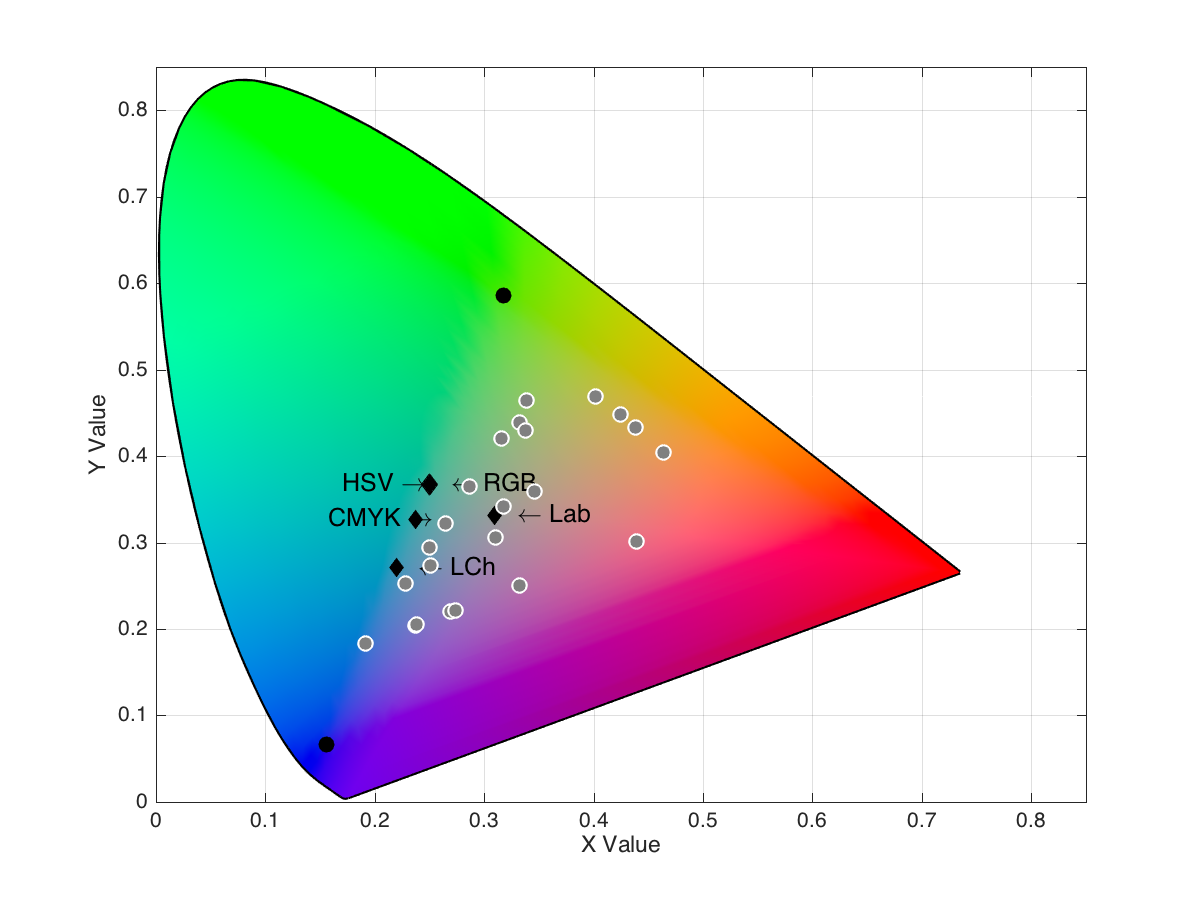
\includegraphics[width=0.48\textwidth]{images/results/20_online_regularUsers.png}
    \caption[Online: Answers for Question 20, from regular users.]{Online: Answers for Question 20, from regular users.}
    \vspace{-15pt}
    \label{fig:onlineregular_20}
  \end{figure}
  %
  \item \ul{Distances} - Comparing the mean distances obtained previously on Table \ref{table:colormodels_distances_labonline_statistics} which were obtained by questions one to seventeen, the distances generated
  by the answers from questions eighteen to thirty-two are a bit higher on the HSV Color Model. However, this could be due to the fact \textbf{we have only presented discretized colors as options, and did not
  leave any wiggle-room for the user to indicate other colors which he thought it could be more appropriate}; moreover, this could be related to \textbf{users tended to explore and choose answers from other color
  models, instead of HSV possible answers}. Even so, the values are similar to the previous studied, being only the HSV and CMYK mean values higher than previously ($\overline{x}_{HSV} = 0.18$, $\overline{x}_{CMYK} = 0.13$).\\
  Blending \ul{Cyan and Yellow to produce green} is an example of a question which had one a higher value ($\overline{x}_{Green = Cyan + Yellow} = 0.11$) when asked the user to indicate the blending-basis with subsequential
  blending in CIE-L*a*b* (question seventeen), and when it was asked the result of the same blending (question nineteen), it provided one of the lowest mean distance values when compared to the ideal CIE-L*a*b* response
  ($\overline{x}_{Cyan + Yellow = Green} = 0.05$); this example if pictured in Figures
  \ref{fig:onlinelabregular_17} and \ref{fig:onlineregular_32}.
  %
  \begin{figure}[!htbp]
    \centering
    \vspace{-15pt}
    \begin{minipage}{0.48\textwidth}
      \centering
      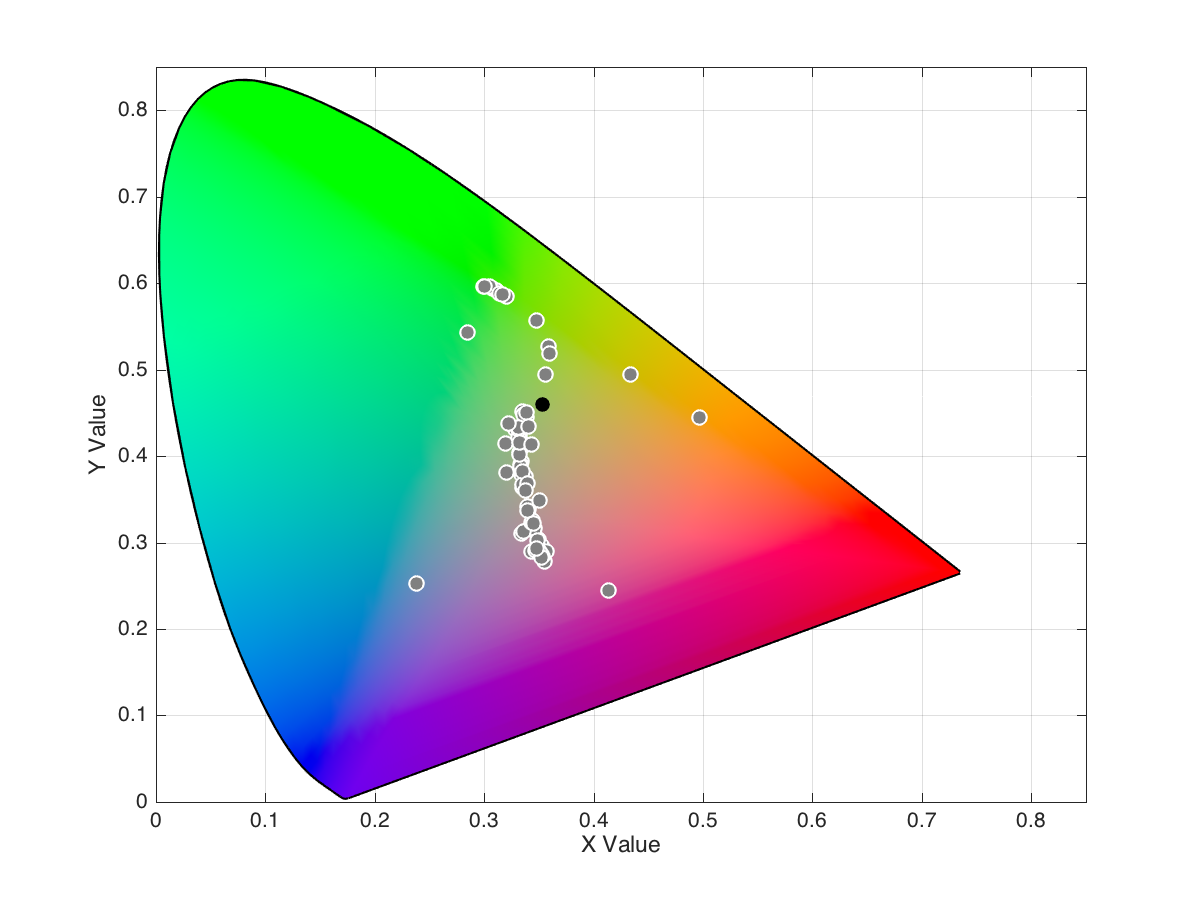
\includegraphics[width=\textwidth]{images/results/17_online_Labresponses.png}
      \caption[Online: Answers for Question 17, from regular users, mixed in CIE-L*a*b* Color Model.]{Online: Answers for Question 17, from regular users, mixed in CIE-L*a*b* Color Model.}
      \label{fig:onlinelabregular_17}
    \end{minipage}\hfill
    \begin{minipage}{0.48\textwidth}
      \centering
      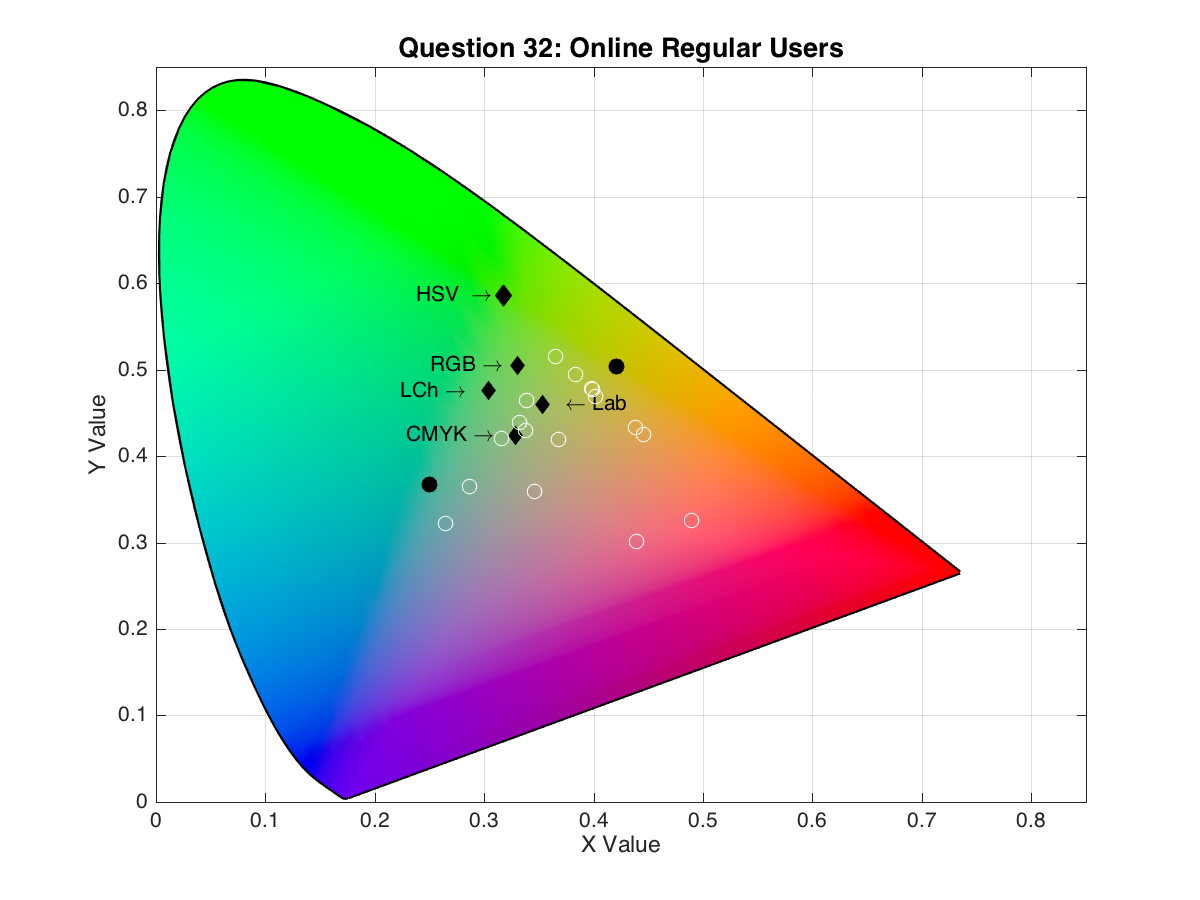
\includegraphics[width=\textwidth]{images/results/32_online_regularUsers.png}
      \caption[Online: Answers for Question 32, from regular users.]{Online: Answers for Question 32, from regular users.}
      \label{fig:onlineregular_32}
    \end{minipage}
    \vspace{-5pt}
  \end{figure}
  %
  \item \ul{Orange Blending} - Comparing the results from all questions, we end up concluding that the question which constantly had best results among all color models was the blending of red and yellow to create
  orange. However, as it is observable, these results represent much higher distances to the ideal answer in any color model, than when given the user the resulting color of the blending. This fact could accuse
  that \textbf{it is harder for the users to detect the result of a color blend, when two blending basis are given, than when the resulting color is given}, even for the orange color blending which produced very good
  results in the previous analysis. This could be related to the lack of descriptive power which the color slider supplied the user, which was referred before. This conclusion is corroborated by the online users which,
  although generating lower mean values than the laboratory ones, are coherent with being higher than the ones previously studied.
  %
  \item \ul{Blue Blending} - Recalling the previous analysis, the results for mixtures which resulted in a blue shade all had the worst results among all questions, across all color models. \emph{Per contra}, the
  results for questions which present a blending basis for creating a blue color had presented much closer distances than before. For example, question twenty-four presented \ul{Cyan and Magenta} seeking a \ul{Blue}
  answer: when the users were asked to indicate the basis (question seven), it generated higher standard deviations which are illustrated in Table \ref{table:colormodels_distances_questions_statistics}. However, as
  seen on Table \ref{table:cyanmagenta_blue_analysis}, the results substantially improve when the users were asked to formulate the result of such blending. \\
  This could potentially suggest that \textbf{according to the users' expectation, it is easier for them to indicate the result of a blue mixture when the blending-basis is given, than when the user is asked
  to create the blending-basis according to their mental color model}.
  %
  \begin{table}[H]
    \resizebox{\textwidth}{!} {
    \begin{tabular}{ccccccccccccc}
      \hline
      \multicolumn{2}{c}{}                                        &                                                          & \multicolumn{10}{c}{Results}                                                                                                                                                                                                                                                                                                                                                                                                                                                                                                                                                             \\ \cline{4-13}
      \multicolumn{2}{c}{\multirow{-2}{*}{Blending Basis}}        & \multirow{-2}{*}{Resulting Color}                        & \multicolumn{2}{c}{HSV}                                                                                              & \multicolumn{2}{c}{CIE-L*C*h}                                                                                        & \multicolumn{2}{c}{CMYK}                                                                                             & \multicolumn{2}{c}{RGB}                                                                                              & \multicolumn{2}{c}{CIE-L*a*b*}                                                               \\ \hline
      Cyan & \multicolumn{1}{c|}{\cellcolor[HTML]{FFFFFF}Magenta} & \multicolumn{1}{c|}{\cellcolor[HTML]{0000FF}{\color[HTML]{FFFFFF}(18, 7, 95)}} & \cellcolor[HTML]{FFFFFF}Laboratory ($\overline{x}$) & \multicolumn{1}{c|}{\cellcolor[HTML]{FFFFFF}Online ($\overline{x}$)} & \cellcolor[HTML]{FFFFFF}Laboratory ($\overline{x}$) & \multicolumn{1}{c|}{\cellcolor[HTML]{FFFFFF}Online ($\overline{x}$)} & \cellcolor[HTML]{FFFFFF}Laboratory ($\overline{x}$) & \multicolumn{1}{c|}{\cellcolor[HTML]{FFFFFF}Online ($\overline{x}$)} & \cellcolor[HTML]{FFFFFF}Laboratory ($\overline{x}$) & \multicolumn{1}{c|}{\cellcolor[HTML]{FFFFFF}Online ($\overline{x}$)} & \cellcolor[HTML]{FFFFFF}Laboratory ($\overline{x}$) & \multicolumn{1}{c|}{Online ($\overline{x}$)} \\ \hline
      \multicolumn{3}{l|}{Given Result, Expected Basis}                                                                      & \textbf{0.16}                                    & \multicolumn{1}{c|}{\textbf{0.13}}                                & 0.23                                             & \multicolumn{1}{c|}{0.18}                                         & 0.10                                             & \multicolumn{1}{c|}{0.11}                                         & 0.15                                             & \multicolumn{1}{c|}{0.17}                                         & 0.17                                             & \multicolumn{1}{c|}{0.22}                 \\
      \multicolumn{3}{l|}{Given Basis, Expected Result}                                                                      & 0.27                                             & \multicolumn{1}{c|}{0.28}                                         & \textbf{0.12}                                    & \multicolumn{1}{c|}{\textbf{0.11}}                                & \textbf{0.08}                                    & \multicolumn{1}{c|}{\textbf{0.09}}                                & \textbf{0.12}                                    & \multicolumn{1}{c|}{\textbf{0.13}}                                & \textbf{0.08}                                    & \multicolumn{1}{c|}{\textbf{0.09}}        \\ \hline
    \end{tabular}}
    \caption[Results of Blending Cyan and Magenta, obtaining Blue.]{Results of Blending Cyan and Magenta, obtaining Blue.}
    \label{table:cyanmagenta_blue_analysis}
  \end{table}
  %
  \item \ul{Color Models Analysis} - There were some changes concerning the descriptive statistics associated with distances values from each color model, specially when discovering which models yielded the best and
  worst results. To help us establish the comparisons between color models, we created an auxiliary Table (\ref{table:colormodels_expectations_labonline_statistics}) which contains the values. Contrary to questions in
  which the user was asked to indicate the blending basis, \textbf{the color model which has the worst results is the HSV Color Model} ($\overline{x}_{HSV} = 0.18$) while the one which has \textbf{the shortest mean distance
  value continues to be CMYK, along with CIE-L*a*b*} ($\overline{x} = 0.13$). Though, when processing the values for the whole statistics, RGB Color Model turns out to be the one which contains the best results: this not only
  is confirmed by the online users' data, but also is contrary to the results from the first analysis which dictated that the best color model was CMYK. This is particularly interesting, since it reveals that \textbf{when
  the users are asked to combine colors after a resulting one is given, they tend to blend according to a subtractive color model (\emph{e.g.} CMYK); but, when the blending-basis is given, the users are likely to mix the colors
  according to an additive color model (\emph{e.g. RGB})}. \\
  On its turn, CIE-L*C*h* continues to reveal itself as the worst-valued Color Model, having the highest standard deviation ($s = 0.07$), the highest range of distances ($range = 0.22$) and the highest variance of values
  ($s^2 = 0.005$), across both study environments.
  %
  \begin{table}[htbp]
    \resizebox{\textwidth}{!} {
    \begin{tabular}{@{}ccccccccccc@{}}
      \toprule
                                                                                         & \multicolumn{5}{c}{Laboratory Environment}                                                                                                                                                                                   & \multicolumn{5}{c}{Online Environment}                                                                                                                                                                               \\ \cmidrule(l){2-11}
      \multirow{-2}{*}{\begin{tabular}[c]{@{}c@{}}Descriptive\\ Statistics\end{tabular}} & HSV                                   & CIE-L*C*h*                             & CMYK                                  & RGB                                    & CIE-L*a*b*                                                 & HSV                                   & CIE-L*C*h*                             & CMYK                                  & RGB                                    & CIE-L*a*b*                                         \\ \midrule
      \multicolumn{1}{c|}{Mean ($\overline{x}$)}                                            & \cellcolor[HTML]{FD6864}\textbf{0.18} & \cellcolor[HTML]{FFFFFF}0.17           & \cellcolor[HTML]{32CB00}\textbf{0.13} & \cellcolor[HTML]{FFFFFF}0.14           & \multicolumn{1}{c|}{\cellcolor[HTML]{32CB00}\textbf{0.13}} & \cellcolor[HTML]{FD6864}\textbf{0.17} & \cellcolor[HTML]{FFFFFF}0.15           & \cellcolor[HTML]{32CB00}\textbf{0.11} & \cellcolor[HTML]{FFFFFF}0.13           & \multicolumn{1}{c|}{\cellcolor[HTML]{FFFFFF}0.12}  \\ \midrule
      \multicolumn{1}{l|}{Std-Dev ($s$)}                                            & \cellcolor[HTML]{FFFFFF}0.06          & \cellcolor[HTML]{FD6864}\textbf{0.07}  & \cellcolor[HTML]{FFFFFF}0.04          & \cellcolor[HTML]{32CB00}\textbf{0.03}  & \multicolumn{1}{c|}{\cellcolor[HTML]{FFFFFF}0.04}          & \cellcolor[HTML]{FD6864}\textbf{0.07} & \cellcolor[HTML]{FD6864}\textbf{0.07}  & \cellcolor[HTML]{FFFFFF}0.04          & \cellcolor[HTML]{32CB00}\textbf{0.03}  & \multicolumn{1}{c|}{\cellcolor[HTML]{FFFFFF}0.04}  \\ \midrule
      \multicolumn{1}{c|}{Maximum Value}                                                 & \cellcolor[HTML]{FFFFFF}0.28          & \cellcolor[HTML]{FFFFFF}0.29           & \cellcolor[HTML]{FFFFFF}0.25          & \cellcolor[HTML]{FFFFFF}0.21           & \multicolumn{1}{c|}{\cellcolor[HTML]{FFFFFF}0.20}          & \cellcolor[HTML]{FFFFFF}0.29          & \cellcolor[HTML]{FFFFFF}0.29           & \cellcolor[HTML]{FFFFFF}0.20          & \cellcolor[HTML]{FFFFFF}0.17           & \multicolumn{1}{c|}{\cellcolor[HTML]{FFFFFF}0.19}  \\ \midrule
      \multicolumn{1}{c|}{Minimum Value}                                                 & \cellcolor[HTML]{FFFFFF}0.11          & \cellcolor[HTML]{FFFFFF}0.07           & \cellcolor[HTML]{FFFFFF}0.08          & \cellcolor[HTML]{FFFFFF}0.09           & \multicolumn{1}{c|}{\cellcolor[HTML]{FFFFFF}0.07}          & \cellcolor[HTML]{FFFFFF}0.09          & \cellcolor[HTML]{FFFFFF}0.07           & \cellcolor[HTML]{FFFFFF}0.07          & \cellcolor[HTML]{FFFFFF}0.07           & \multicolumn{1}{c|}{\cellcolor[HTML]{FFFFFF}0.05}  \\ \midrule
      \multicolumn{1}{c|}{Range}                                                         & \cellcolor[HTML]{FFFFFF}0.17          & \cellcolor[HTML]{FD6864}\textbf{0.22}  & \cellcolor[HTML]{FFFFFF}0.17          & \cellcolor[HTML]{32CB00}\textbf{0.12}  & \multicolumn{1}{c|}{\cellcolor[HTML]{FFFFFF}0.13}          & \cellcolor[HTML]{FFFFFF}0.20          & \cellcolor[HTML]{FD6864}\textbf{0.22}  & \cellcolor[HTML]{FFFFFF}0.13          & \cellcolor[HTML]{32CB00}\textbf{0.10}  & \multicolumn{1}{c|}{\cellcolor[HTML]{FFFFFF}0.14}  \\ \midrule
      \multicolumn{1}{c|}{Variance ($s^2$)}                                         & \cellcolor[HTML]{FFFFFF}0.003         & \cellcolor[HTML]{FD6864}\textbf{0.005} & \cellcolor[HTML]{FFFFFF}0.002         & \cellcolor[HTML]{32CB00}\textbf{0.001} & \multicolumn{1}{c|}{\cellcolor[HTML]{FFFFFF}0.002}         & \cellcolor[HTML]{FFFFFF}0.004         & \cellcolor[HTML]{FD6864}\textbf{0.005} & \cellcolor[HTML]{FFFFFF}0.002         & \cellcolor[HTML]{32CB00}\textbf{0.001} & \multicolumn{1}{c|}{\cellcolor[HTML]{FFFFFF}0.002} \\ \bottomrule
    \end{tabular}}
    \caption[Condensed Statistics for Distances to Ideal Results, according to each Color Model, for questions 18 to 32.]{Condensed Statistics for Distances to Ideal Results, according to each Color Model, for questions 18 to 32. In Green/Red shade, the best/worst result for each descriptive statistic.}
    \label{table:colormodels_expectations_labonline_statistics}
  \end{table}
  %
\end{itemize} \par
%
Therefore, we can summarize the results in one table, which ranks the color models \emph{per} color blending, dividing it between two strands: based on the values that represent questions in which the user was
asked to indicate the blending-basis, and based on the values that represent questions in which the user was asked to point out the correct blending result when given two colors. These results are presented in
Table \ref{table:blendings_models_rank}. The color models were ranked according to the descriptive statistics' values generated by each question, weighted with the results from the laboratory environment and the
validation from the online users: for each question, we started by searching for the lowest mean value from the laboratory values, then comparing it with its correspondent from the online environment to validate
it; if there was any tie between values from the same environment, \textbf{the untie would be done by evaluating the standard deviations} and it would be chosen the color model which had the lowest value. If the
untie was not possible, then \textbf{we did not have enough information to state which color model was better than another}. \par
%
For example, we performed the following evaluation for \textbf{question four} values:
%
\begin{enumerate}
  \item On the laboratory environment, the color model which had \ul{the lowest mean} value was \textbf{CMYK} ($\overline{x}_{CMYK} = 0.10$); the same for the online environment ($\overline{x}_{CMYK} = 0.11$).
  \item On the laboratory environment, the color model which had \ul{the second lowest mean} value was \textbf{HSV} ($\overline{x}_{HSV} = 0.12$); the same for the online environment ($\overline{x}_{HSV} = 0.11$).
  \item On the laboratory environment, the color model which had \ul{the third lowest mean} value was \textbf{RGB} ($\overline{x}_{RGB} = 0.19$); the same for the online environment ($\overline{x}_{RGB} = 0.21$).
  \item Lastly, there were two color models which had the highest mean values, on the laboratory environment: \textbf{CIE-L*a*b* and CIE-L*C*h*} ($\overline{x} = 0.20$); however, the value from the online environment
  was lower for CIE-L*C*h* Color Model ($\overline{x}_{LCh} = 0.22$), than the CIE-L*a*b*.
  \item Therefore, we conclude that the color models can be ranked in the following order, \ul{according to their descriptive statistics}: \textbf{CMYK, HSV, RGB, CIE-L*C*h* and CIE-L*a*b*}.
\end{enumerate}
%
Marked in \textbf{bold}, on Table \ref{table:blendings_models_rank}, are the color models which we have concluded to yield the best results, according to each type of question asked: \textbf{CMYK} when given the
result and asked for the blending-basis, and \textbf{CMYK and RGB} for the questions whose blending-basis was given and the result was asked. For the blends of Magenta-Yellow and Blue-Cyan, we did not found
conclusive results, as referred before: for the first one, it was not possible to concretely state which color model was the best, since all color models yielded similar closer distances; for the later blending, it was possible
to concretely affirm which color model was the best or worst, since all color models provided higher distances, very similar between each other.
%
\begin{table}[htbp]
  \resizebox{\textwidth}{!} {
  \begin{tabular}{@{}ccclcccccccccc@{}}
  \toprule
  \multicolumn{2}{c}{Blending Basis}                                       & \multicolumn{2}{c}{Blending Result}                        & \multicolumn{5}{c}{Given the Result, Asked for Basis}                                                                                                                                                 & \multicolumn{5}{c}{Given the Basis, Asked for Result}                                                                                                                                                                                                                   \\ \midrule
    C1                      & C2                                             & \multicolumn{2}{c|}{C3}                                    & \#1                                                        & \#2                                & \#3                             & \#4                             & \multicolumn{1}{c|}{\#5}        & \#1                                                  & \#2                                                  & \#3                                               & \#4                                               & \multicolumn{1}{c|}{\#5}                          \\ \midrule
    Red                     & \multicolumn{1}{c|}{Green}                     & \multicolumn{2}{c|}{\cellcolor[HTML]{FFFF00}(77, 93, 14)}  & \multicolumn{1}{c|}{\textbf{CMYK}}                         & \multicolumn{1}{c|}{CIE-L*a*b*}    & \multicolumn{1}{c|}{RGB}        & \multicolumn{1}{c|}{HSV}        & \multicolumn{1}{c|}{CIE-L*C*h*} & \multicolumn{1}{c|}{\textbf{CMYK}}                   & \multicolumn{1}{c|}{CIE-L*a*b*}                      & \multicolumn{1}{c|}{HSV}                          & \multicolumn{1}{c|}{\textbf{RGB}}                 & \multicolumn{1}{c|}{CIE-L*C*h*}                   \\ \midrule
    Red                     & \multicolumn{1}{c|}{Blue}                      & \multicolumn{2}{c|}{\cellcolor[HTML]{FF00FF}(59, 28, 97)}  & \multicolumn{1}{c|}{\textbf{CMYK}}                         & \multicolumn{1}{c|}{CIE-L*a*b*}    & \multicolumn{1}{c|}{CIE-L*C*h*} & \multicolumn{1}{c|}{RGB}        & \multicolumn{1}{c|}{HSV}        & \multicolumn{1}{c|}{HSV}                             & \multicolumn{1}{c|}{\textbf{RGB}}                    & \multicolumn{1}{c|}{\textbf{CMYK}}                & \multicolumn{1}{c|}{CIE-L*a*b*}                   & \multicolumn{1}{c|}{CIE-L*C*h*}                   \\ \midrule
    Green                   & \multicolumn{1}{c|}{Blue}                      & \multicolumn{2}{c|}{\cellcolor[HTML]{00FFFF}(54, 79, 107)} & \multicolumn{5}{c|}{-}                                                                                                                                                                                & \multicolumn{1}{c|}{CIE-L*a*b*}                      & \multicolumn{2}{c|}{\textbf{HSV, RGB}}                                                                   & \multicolumn{1}{c|}{\textbf{CMYK}}                & \multicolumn{1}{c|}{CIE-L*C*h*}                   \\ \midrule
                            & \multicolumn{1}{c|}{}                          & \multicolumn{2}{c|}{\cellcolor[HTML]{80FF00}(45, 76, 12)}  & \multicolumn{1}{c|}{\textbf{CMYK}}                         & \multicolumn{1}{c|}{HSV}           & \multicolumn{1}{c|}{RGB}        & \multicolumn{1}{c|}{CIE-L*a*b*} & \multicolumn{1}{c|}{CIE-L*C*h*} & \multicolumn{1}{c|}{}                                & \multicolumn{1}{c|}{}                                & \multicolumn{1}{c|}{}                             & \multicolumn{1}{c|}{}                             & \multicolumn{1}{c|}{}                             \\ \cmidrule(lr){3-9}
    \multirow{-2}{*}{Red}   & \multicolumn{1}{c|}{\multirow{-2}{*}{Cyan}}    & \multicolumn{2}{c}{\cellcolor[HTML]{7F00FF}(27, 12, 95)}   & \multicolumn{1}{c|}{\textbf{CMYK}}                         & \multicolumn{1}{c|}{HSV}           & \multicolumn{1}{c|}{RGB}        & \multicolumn{1}{c|}{CIE-L*C*h*} & \multicolumn{1}{c|}{CIE-L*a*b*} & \multicolumn{1}{c|}{\multirow{-2}{*}{\textbf{RGB}}}  & \multicolumn{1}{c|}{\multirow{-2}{*}{\textbf{CMYK}}} & \multicolumn{1}{c|}{\multirow{-2}{*}{CIE-L*a*b*}} & \multicolumn{1}{c|}{\multirow{-2}{*}{HSV}}        & \multicolumn{1}{c|}{\multirow{-2}{*}{CIE-L*C*h*}} \\ \midrule
    Red                     & \multicolumn{1}{c|}{Magenta}                   & \multicolumn{2}{c|}{\cellcolor[HTML]{FF0080}(45, 23, 22)}  & \multicolumn{1}{c|}{\textbf{CMYK}}                         & \multicolumn{3}{c|}{CIE-L*C*h*, CIE-L*a*b*, RGB}                                                       & \multicolumn{1}{c|}{HSV}        & \multicolumn{1}{c|}{HSV}                             & \multicolumn{1}{c|}{CIE-L*C*h*, CIE-L*a*b*}          & \multicolumn{1}{c|}{}                             & \multicolumn{1}{c|}{\textbf{RGB}}                 & \multicolumn{1}{c|}{\textbf{CMYK}}                \\ \midrule
    Red                     & \multicolumn{1}{c|}{Yellow}                    & \multicolumn{2}{c|}{\cellcolor[HTML]{FF8000}(49, 37, 5)}   & \multicolumn{1}{c|}{CIE-L*a*b*}                            & \multicolumn{3}{c|}{\textbf{CMYK, HSV, RGB}}                                                           & \multicolumn{1}{c|}{CIE-L*C*h*} & \multicolumn{3}{c|}{\textbf{CMYK, CIE-L*C*h*, CIE-L*a*b*}}                                                                                                      & \multicolumn{1}{c|}{HSV}                          & \multicolumn{1}{c|}{\textbf{RGB}}                 \\ \midrule
    Cyan                    & \multicolumn{1}{c|}{Magenta}                   & \multicolumn{2}{c|}{\cellcolor[HTML]{0000FF}(18, 7, 95)}   & \multicolumn{1}{c|}{\textbf{CMYK}}                                  & \multicolumn{1}{c|}{RGB}           & \multicolumn{1}{c|}{HSV}        & \multicolumn{1}{c|}{CIE-L*a*b*} & \multicolumn{1}{c|}{CIE-L*C*h*} & \multicolumn{2}{c|}{\textbf{CMYK, CIE-L*a*b*}}                                                              & \multicolumn{1}{c|}{CIE-L*C*h*}                   & \multicolumn{1}{c|}{\textbf{RGB}}                 & \multicolumn{1}{c|}{HSV}                          \\ \midrule
    Magenta                 & \multicolumn{1}{c|}{Yellow}                    & \multicolumn{2}{c|}{\cellcolor[HTML]{FF0000}(41, 21, 2)}   & \multicolumn{5}{c|}{Inconclusive Results}                                                                                                                                                             & \multicolumn{1}{c|}{CIE-L*a*b*}                      & \multicolumn{1}{c|}{\textbf{CMYK}}                   & \multicolumn{1}{c|}{\textbf{RGB}}                 & \multicolumn{1}{c|}{CIE-L*C*h*}                   & \multicolumn{1}{c|}{HSV}                          \\ \midrule
    Green                   & \multicolumn{1}{c|}{Cyan}                      & \multicolumn{2}{c|}{\cellcolor[HTML]{00FF80}(40, 73, 32)}  & \multicolumn{1}{c|}{\textbf{CMYK}}                         & \multicolumn{1}{c|}{RGB}           & \multicolumn{1}{c|}{CIE-L*a*b*} & \multicolumn{1}{c|}{HSV}        & \multicolumn{1}{c|}{CIE-L*C*h*} & \multicolumn{1}{c|}{CIE-L*C*h*}                      & \multicolumn{1}{c|}{\textbf{CMYK}}                   & \multicolumn{1}{c|}{CIE-L*a*b*}                   & \multicolumn{1}{c|}{HSV}                          & \multicolumn{1}{c|}{\textbf{RGB}}                 \\ \midrule
                            & \multicolumn{1}{c|}{}                          & \multicolumn{2}{c|}{\cellcolor[HTML]{0080FF}(26, 23, 98)}  & \multicolumn{1}{c|}{\cellcolor[HTML]{FFFFFF}\textbf{CMYK}} & \multicolumn{1}{c|}{RGB}           & \multicolumn{1}{c|}{CIE-L*a*b*} & \multicolumn{1}{c|}{HSV}        & \multicolumn{1}{c|}{CIE-L*C*h*} & \multicolumn{1}{c|}{}                                & \multicolumn{1}{c|}{}                                & \multicolumn{1}{c|}{}                             & \multicolumn{1}{c|}{}                             & \multicolumn{1}{c|}{}                             \\ \cmidrule(lr){3-9}
    \multirow{-2}{*}{Green} & \multicolumn{1}{c|}{\multirow{-2}{*}{Magenta}} & \multicolumn{2}{c}{\cellcolor[HTML]{FF8000}(49, 37, 5)}    & \multicolumn{1}{c|}{HSV}                                   & \multicolumn{1}{c|}{\textbf{CMYK}} & \multicolumn{1}{c|}{CIE-L*C*h*} & \multicolumn{1}{c|}{CIE-L*a*b*} & \multicolumn{1}{c|}{RGB}        & \multicolumn{1}{c|}{\multirow{-2}{*}{\textbf{RGB}}}  & \multicolumn{1}{c|}{\multirow{-2}{*}{\textbf{CMYK}}} & \multicolumn{1}{c|}{\multirow{-2}{*}{CIE-L*a*b*}} & \multicolumn{1}{c|}{\multirow{-2}{*}{HSV}}        & \multicolumn{1}{c|}{\multirow{-2}{*}{CIE-L*C*h*}} \\ \midrule
    Green                   & \multicolumn{1}{c|}{Yellow}                    & \multicolumn{2}{c|}{\cellcolor[HTML]{80FF00}(45, 76, 12)}  & \multicolumn{1}{c|}{HSV}                                   & \multicolumn{1}{c|}{\textbf{CMYK}} & \multicolumn{1}{c|}{RGB}        & \multicolumn{1}{c|}{CIE-L*a*b*} & \multicolumn{1}{c|}{CIE-L*C*h*} & \multicolumn{1}{c|}{\textbf{CMYK}}                   & \multicolumn{1}{c|}{CIE-L*C*h*, CIE-L*a*b*}          & \multicolumn{1}{c|}{}                             & \multicolumn{1}{c|}{\textbf{RGB}}                 & \multicolumn{1}{c|}{HSV}                          \\ \midrule
    Blue                    & \multicolumn{1}{c|}{Cyan}                      & \multicolumn{2}{c|}{\cellcolor[HTML]{0080FF}(26, 23, 98)}  & \multicolumn{5}{c|}{Inconclusive Results}                                                                                                                                                             & \multicolumn{1}{c|}{CIE-L*C*h*}                      & \multicolumn{1}{c|}{CIE-L*a*b*}                      & \multicolumn{1}{c|}{\textbf{CMYK}}                & \multicolumn{2}{c|}{\textbf{HSV, RGB}}                                                                \\ \midrule
    Blue                    & \multicolumn{1}{c|}{Magenta}                   & \multicolumn{2}{c|}{\cellcolor[HTML]{8000FF}(27, 12, 95)}  & \multicolumn{1}{c|}{\textbf{CMYK}}                         & \multicolumn{1}{c|}{HSV}           & \multicolumn{1}{c|}{RGB}        & \multicolumn{1}{c|}{CIE-L*a*b*} & \multicolumn{1}{c|}{CIE-L*C*h*} & \multicolumn{2}{c|}{CIE-L*C*h*, CIE-L*a*b*}                                                                 & \multicolumn{1}{c|}{\textbf{CMYK}}                & \multicolumn{1}{c|}{\textbf{RGB}}                 & \multicolumn{1}{c|}{HSV}                          \\ \midrule
                            & \multicolumn{1}{c|}{}                          & \multicolumn{2}{c|}{\cellcolor[HTML]{00FF80}(40, 73, 32)}  & \multicolumn{1}{c|}{\textbf{CMYK}}                         & \multicolumn{1}{c|}{HSV}           & \multicolumn{1}{c|}{RGB}        & \multicolumn{1}{c|}{CIE-L*a*b*} & \multicolumn{1}{c|}{CIE-L*C*h*} & \multicolumn{1}{c|}{}                                & \multicolumn{1}{c|}{}                                & \multicolumn{1}{c|}{}                             & \multicolumn{1}{c|}{}                             & \multicolumn{1}{c|}{}                             \\ \cmidrule(lr){3-9}
    \multirow{-2}{*}{Blue}  & \multicolumn{1}{c|}{\multirow{-2}{*}{Yellow}}  & \multicolumn{2}{c|}{\cellcolor[HTML]{FF007F}(45, 23, 22)}  & \multicolumn{1}{c|}{\textbf{CMYK}}                         & \multicolumn{1}{c|}{CIE-L*a*b*}    & \multicolumn{1}{c|}{RGB}        & \multicolumn{1}{c|}{HSV}        & \multicolumn{1}{c|}{CIE-L*C*h*} & \multicolumn{1}{c|}{\multirow{-2}{*}{\textbf{CMYK}}} & \multicolumn{1}{c|}{\multirow{-2}{*}{\textbf{RGB}}}  & \multicolumn{1}{c|}{\multirow{-2}{*}{HSV}}        & \multicolumn{1}{c|}{\multirow{-2}{*}{CIE-L*a*b*}} & \multicolumn{1}{c|}{\multirow{-2}{*}{CIE-L*C*h*}} \\ \midrule
    Cyan                    & \multicolumn{1}{c|}{Yellow}                    & \multicolumn{2}{c|}{\cellcolor[HTML]{00FF00}(36, 72, 13)}  & \multicolumn{1}{c|}{\textbf{CMYK}}                         & \multicolumn{1}{c|}{HSV}           & \multicolumn{1}{c|}{RGB}        & \multicolumn{1}{c|}{CIE-L*a*b*} & \multicolumn{1}{c|}{CIE-L*C*h*} & \multicolumn{1}{c|}{CIE-L*a*b*}                      & \multicolumn{1}{c|}{\textbf{CMYK}}                   & \multicolumn{1}{c|}{CIE-L*C*h*}                   & \multicolumn{1}{c|}{\textbf{RGB}}                 & \multicolumn{1}{c|}{HSV}                          \\ \bottomrule
  \end{tabular}}
  \caption[Colors Models, ranked from best to worst, associated to every color blending studied.]{Colors Models, ranked from best to worst, associated to every color blending studied.}
  \label{table:blendings_models_rank}
\end{table}
%
\subsection{Color Mixtures and Color Naming}
\label{subsec:results_colormixtures}
%
Being the color models covered in the extensive previous analysis, we are left to analyze and break down each color mixture, understanding if there is a particular color blending which has an added level of
difficulty. As stated on Section \ref{sec:impl_objectives}, it is also interesting to study if the users have a particular choice to order the colors when demonstrating their answers, given its implications on how to draft \ul{Information Visualization Artifacts},
such as sliders, scales or color blends to convey information.
%
This subSection will be composed on two main groups: on the first one, we will focus our attention on the color blendings which are \textbf{based on primary colors, to generate other primary colors} to comprehend
if the users can detect and formulate primary color blendings; the second group of this subSection will contain a \textbf{brief investigation about the difficulty found when blending colors}, focusing our attention
not only on each question, but also on providing a general perception of how the study went, regarding the facility of unveiling color mixtures. \par
%
We also performed a color analysis by comparing the colors given by our users, with the ones obtained with the XKCD's Color Bins referred on the \emph{Data Processing} Section (\ref{subsec:results_preparation}) of this document. This way,
we can make sense out of the values, giving them meaning and necessary categorization. This is going to be useful when analyzing the proximity of values.
%
\subsubsection{Primary Colors}
\label{subsubsec:primarycolors}
%
Among all the questions proponed to the user, there were of six of them which presented as the result of a color mixture, either one of the following primary colors: \textbf{Red, Green, Blue, Cyan, Magenta,}
or \textbf{Yellow}. These results are the primitives from one additive color model (RGB) and one subtractive color model (CMYK): what we intend to know is if the user is capable of creating color blendings
which result in these colors; since these color models are complementary, the user must reveal knowledge of mixing colors according to these two models, while creating blendings with colors from the opposite
color model. These questions are refreshed again on Table \ref{table:primary_blends}. \par
%
\begin{table}[htbp]
  \resizebox{\textwidth}{!} {
  \begin{tabular}{ccccclclclclcl}
    \hline
                                  & \multicolumn{2}{c}{Blending Basis}                          &                                                                          & \multicolumn{10}{c}{Possible Results}                                                                                                                                                                                                                                                                                                                                                                 \\ \cline{2-3} \cline{5-14}
    \multirow{-2}{*}{Question ID} & C1                           & C2                           & \multirow{-2}{*}{Blending Result}                                        & \multicolumn{2}{c}{HSV}                                                         & \multicolumn{2}{c}{CIE-L*C*h}                                                    & \multicolumn{2}{c}{CMYK}                                                         & \multicolumn{2}{c}{RGB}                                                          & \multicolumn{2}{c}{CIE-L*a*b*}                             \\ \hline
    \multicolumn{1}{c|}{8, 25}    & \multicolumn{1}{c|}{Magenta} & \multicolumn{1}{c||}{Yellow}  & \multicolumn{1}{c||}{\cellcolor[HTML]{FF0000}{\color[HTML]{FFFFFF} Red}}  & \multicolumn{2}{c||}{\cellcolor[HTML]{FF0000}{\color[HTML]{FFFFFF} (41, 21, 2)}} & \multicolumn{2}{c||}{\cellcolor[HTML]{FF6755}{\color[HTML]{FFFFFF} (48, 32, 12)}} & \multicolumn{2}{c||}{\cellcolor[HTML]{FF8080}{\color[HTML]{FFFFFF} (53, 38, 25)}} & \multicolumn{2}{c||}{\cellcolor[HTML]{FF8080}{\color[HTML]{FFFFFF} (53, 38, 25)}} & \multicolumn{2}{c|}{\cellcolor[HTML]{FFA6A6}(62, 51, 43)}  \\ \hline \hline
    \multicolumn{1}{c|}{17, 32}   & \multicolumn{1}{c|}{Cyan}    & \multicolumn{1}{c||}{Yellow}  & \multicolumn{1}{c||}{\cellcolor[HTML]{00FF00}Green}                       & \multicolumn{2}{c||}{\cellcolor[HTML]{00FF00}(36, 72, 13)}                       & \multicolumn{2}{c||}{\cellcolor[HTML]{6EFFA3}(49, 77, 47)}                        & \multicolumn{2}{c||}{\cellcolor[HTML]{80FF80}(49, 78, 33)}                        & \multicolumn{2}{c||}{\cellcolor[HTML]{80FF80}(49, 78, 33)}                        & \multicolumn{2}{c|}{\cellcolor[HTML]{C4FF9E}(66, 87, 46)}  \\ \hline \hline
    \multicolumn{1}{c|}{7, 24}    & \multicolumn{1}{c|}{Cyan}    & \multicolumn{1}{c||}{Magenta} & \multicolumn{1}{c||}{\cellcolor[HTML]{0000FF}{\color[HTML]{FFFFFF} Blue}} & \multicolumn{2}{c||}{\cellcolor[HTML]{0000FF}{\color[HTML]{FFFFFF} (18, 7, 95)}} & \multicolumn{2}{c||}{\cellcolor[HTML]{00CAFF}(39, 49, 102)}                       & \multicolumn{2}{c||}{\cellcolor[HTML]{8080FF}{\color[HTML]{FFFFFF} (35, 27, 98)}} & \multicolumn{2}{c||}{\cellcolor[HTML]{8080FF}{\color[HTML]{FFFFFF} (35, 27, 98)}} & \multicolumn{2}{c|}{\cellcolor[HTML]{C6AEFF}(56, 50, 101)} \\ \hline \hline
    \multicolumn{1}{c|}{20}       & \multicolumn{1}{c|}{Green}   & \multicolumn{1}{c||}{Blue}    & \multicolumn{1}{c||}{\cellcolor[HTML]{00FFFF}Cyan}                        & \multicolumn{2}{c||}{\cellcolor[HTML]{00FFFF}(54, 79, 107)}                      & \multicolumn{2}{c||}{\cellcolor[HTML]{00A5FF}(32, 34, 100)}                       & \multicolumn{2}{c||}{\cellcolor[HTML]{008080}(12, 17, 23)}                        & \multicolumn{2}{c||}{\cellcolor[HTML]{008080}(12, 17, 23)}                        & \multicolumn{2}{c|}{\cellcolor[HTML]{7D93A6}(26, 28, 40)}  \\ \hline \hline
    \multicolumn{1}{c|}{2, 19}    & \multicolumn{1}{c|}{Red}     & \multicolumn{1}{c||}{Blue}    & \multicolumn{1}{c||}{\cellcolor[HTML]{FF00FF}Magenta}                     & \multicolumn{2}{c||}{\cellcolor[HTML]{FF00FF}(59, 28, 97)}                       & \multicolumn{2}{c||}{\cellcolor[HTML]{FB0080}{\color[HTML]{FFFFFF} (44, 22, 22)}} & \multicolumn{2}{c||}{\cellcolor[HTML]{800080}{\color[HTML]{FFFFFF} (13, 6, 21)}}  & \multicolumn{2}{c||}{\cellcolor[HTML]{800080}{\color[HTML]{FFFFFF} (13, 6, 21)}}  & \multicolumn{2}{c|}{\cellcolor[HTML]{CA0088}(29, 14, 25)}  \\ \hline \hline
    \multicolumn{1}{c|}{1, 18}    & \multicolumn{1}{c|}{Red}     & \multicolumn{1}{c||}{Green}   & \multicolumn{1}{c||}{\cellcolor[HTML]{FFFF00}Yellow}                      & \multicolumn{2}{c||}{\cellcolor[HTML]{FFFF00}(77, 93, 14)}                       & \multicolumn{2}{c||}{\cellcolor[HTML]{D7A700}(42, 42, 6)}                         & \multicolumn{2}{c||}{\cellcolor[HTML]{808000}(17, 20, 3)}                         & \multicolumn{2}{c||}{\cellcolor[HTML]{808000}(17, 20, 3)}                         & \multicolumn{2}{c|}{\cellcolor[HTML]{C9AB00}(39, 42, 6)}   \\ \hline
  \end{tabular}}
  \caption[Color Blends based on Primary Colors, which result in other Primary Colors.]{Color Blends based on Primary Colors, which result in other Primary Colors.}
  \label{table:primary_blends}
\end{table}
%
As analyzed before, according to the users' responses and expectations, these questions show a fair degree of concordance when blending the mixture-basis, since they all tend tend to present better results when
blended according to a CMYK Color Model. However, we have found an interesting behavior from our users when answering these questions: some users indicated the resulting color on both the reference pairs (\emph{e.g.}
Red was presented, and the users indicated twice the color Red in their answers); we will briefly analyze the values for each of the blendings referred on Table \ref{table:primary_blends}, as it has already been
analyzed before.
%
\paragraph{\ul{Magenta + Yellow = Red}}
%
In this question, it was expected that users indicate a mixing of Magenta and Yellow to blend in a result of Red. These colors are primitives from the CMYK Color Model which, when blended, generate a color from the
complementary color model, the RGB. However, the laboratory users did focus their answers on \textbf{orange, green, blue and even red hue}; moreover, these results were similar among the online users and did not
demonstrated a consensual answer pair. \\
%
Additionally, five laboratory users (from thirteen which indicated a pair of two answers - $38.46\%$ of the users) and forty-two online users (from sixty-two - $67.74\%$ of the users) indicated, at least, one time the
red color as an answer. We can even run some descriptive statistics on top of the \ul{distance values between the given answers and the expected Magenta-Yellow Pair} ($\overline{x} = 0.49$, $s = 0.25$) and observe that
these evidences lead us to believe that \textbf{the users do not know how to create a red color based on other primary colors}. \\
%
When analyzing question number twenty-five, in which we ask the user which color is the result of blending Magenta and Yellow, we conclude that \textbf{the results are, also,
scattered a bit}, which leads us to reinforce the statement above. \textbf{There is also no observable tendency to begin the color blending with a particular shade of a color}. Figures \ref{fig:redblend_1} and
\ref{fig:redblend_2} show us the answers given by the online users in, respectively, question eight and twenty-five. \\
%
Finally, since we have produced the mapping between given values and color bins, we can perform a qualitative analysis of
each answer pair's colors names while comparing it to the expected ones. The expected pair was \ul{Magenta-Yellow}: among
62 answers from the online users to question 8, \textbf{we conclude that the colors Magenta and Yellow were among the least
indicated ones}, being Magenta indicated four times and five times. The most repeated color was Red, being indicated more than
70 times: there were 31 answer-pairs ($50\%$) which contained the color Red twice! When given by the user, the Magenta was combined
with Green and Red, while Yellow was combined with Red, Green and Blue; however, the specific pair Magenta-Yellow was never indicated.
%
\begin{figure}[!htbp]
  \centering
  \begin{minipage}{0.48\textwidth}
    \centering
    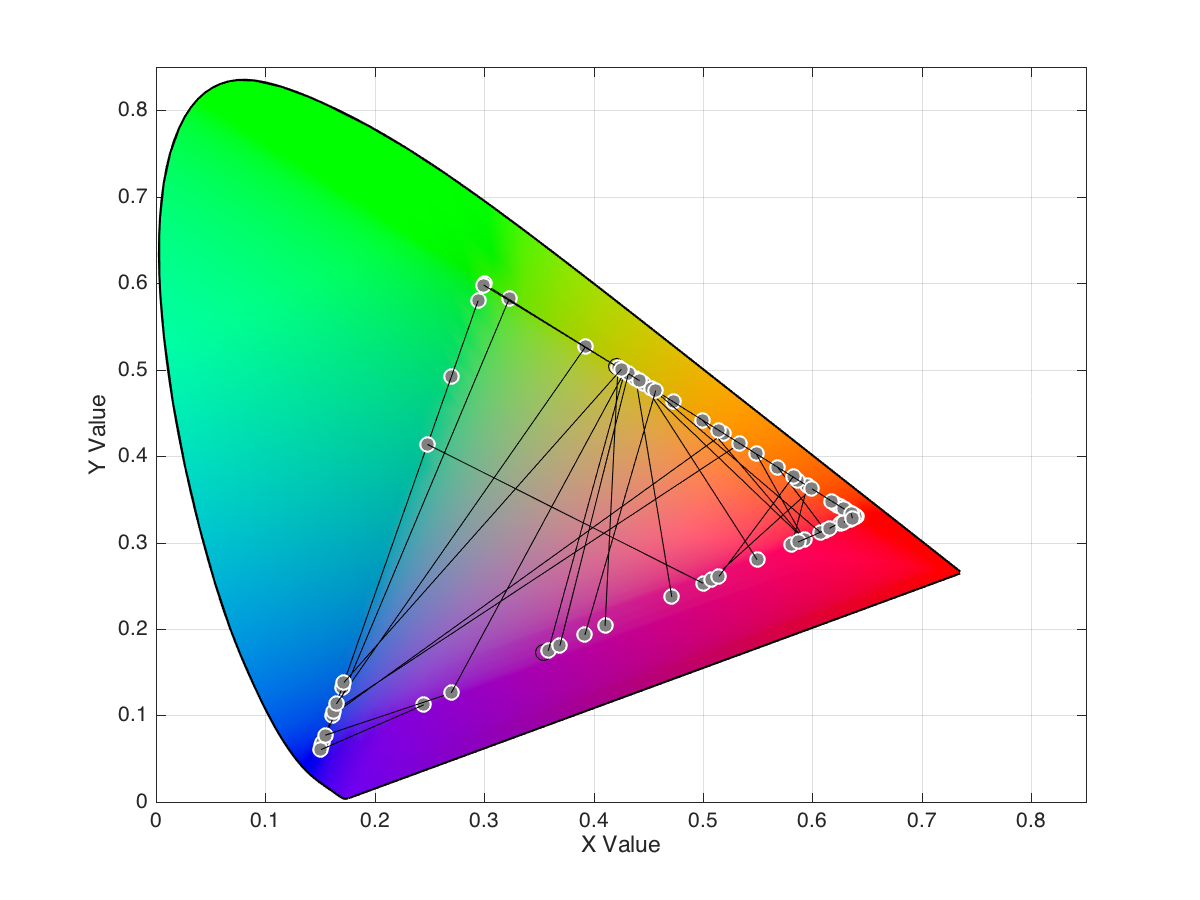
\includegraphics[width=\textwidth]{images/results/8_online_regularUsers.png}
    \caption[Online: Answers for Question 8, from regular users.]{Online: Answers for Question 8, from regular users.}
    \label{fig:redblend_1}
  \end{minipage}\hfill
  \begin{minipage}{0.48\textwidth}
    \centering
    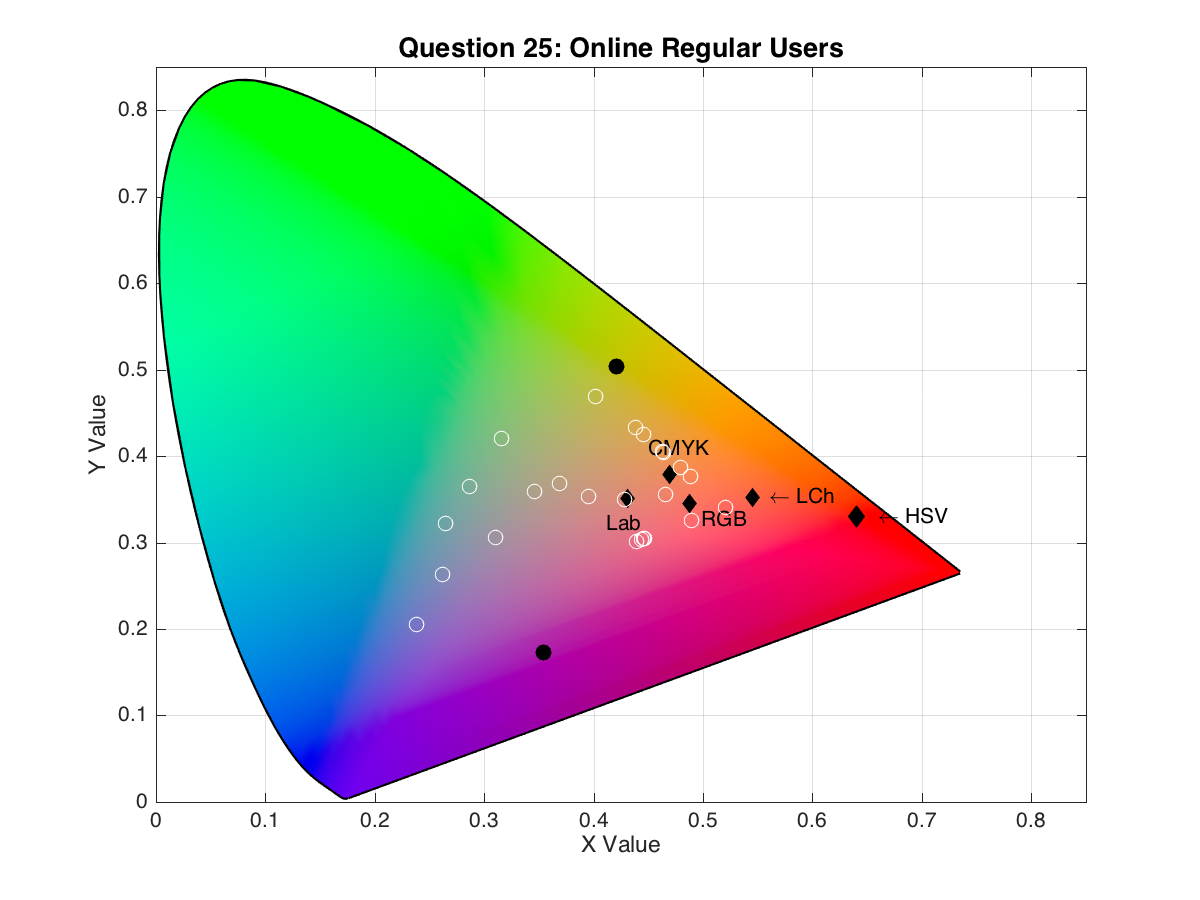
\includegraphics[width=\textwidth]{images/results/25_online_regularUsers.png}
    \caption[Online: Answers for Question 25, from regular users.]{Online: Answers for Question 25, from regular users.}
    \label{fig:redblend_2}
  \end{minipage}
\end{figure}
%
\paragraph{\ul{Cyan + Yellow = Green}}
%
Regarding this, it was expected that users indicate a mixing of Cyan and Yellow to blend in a result of Green. Similarly to the previous blend, these colors are primitives from the CMYK Color Model that, when blended,
generate a color from the RGB Color Model. Curiously, both the laboratory and online users provided their answers on similar pairs, comprised between \textbf{blue shades and yellow ones}; the most repeated
color pairs were, in fact, Blue shades combined with tones of green and yellow, as observable on Figure \ref{fig:greenblend_1}. \\
%
Additionally, only two laboratory users (from twenty-three which indicated a pair of two answers - $8.70\%$ of the users) and six online users (from seventy-one - $8.45\%$ of the users) indicated an answer pair which did not even
nearly approximate to the desired hues. Running some descriptive statistics on top of the distance values between the given answers and the expected Magenta-Yellow Pair ($\overline{x} = 0.40$, $s = 0.21$) did reveal longer distances
also; however, since the majority of answers are near a cyan hue tending to a blue one, we consider these answers as valid ones. These evidences lead us to believe that \textbf{the users do present knowledge on how to create a green color
based on other primary colors, such as cyan/blue and yellow}. \\
%
When analyzing question number thirty-two, in which we ask the user which color is the result of blending Cyan and Yellow, we conclude that \textbf{the results, as previously happened with other primary blends, are a bit scattered}.
As before, \textbf{there is no observable tendency to begin the color blending with a particular shade of a color}. Figures \ref{fig:greenblend_2} and\ref{fig:greenblend_2} show us the answers given by the online users in, respectively,
question seventeen and thirty-two. \\
%
We can perform a qualitative analysis of each answer pair's colors names while comparing it to the expected ones. The
expected pair was \ul{Cyan and Yellow}: among 71 answers from the online users to question 17, \textbf{we conclude
that the color Yellow was among the least indicated ones}; however, users have diverged a little when indicating the cyan
color, since \textbf{the users have answered with colors varying between Blue, Navy-Blue, Sky-Blue, Light-Blue and Teal}, with frequencies
of 37, 11, 3, 1 and 1 respectively, while Cyan was only referred 4 times. Though, users have referenced a lot more times the
Green color, which is the presented one: 77 times to be more precise, with \textbf{53 answer-pairs formed with a Blue shade and Green} ($75\%$ of the
totality of pairs) and 10 pairs which contained the Green color twice. If analyzed, the CIE Chromaticity Diagram in Figure \ref{fig:greenblend_1} consolidates
this idea, revealing the dispersion of blue derived colors' usage, but a slight concentration of answers in the neighborhood of Green and Yellow.
Regarding the latter color, it was combined 4 times with blue shades which is another indicator that \textbf{users presented strong Blue-Green/Yellow blending
capabilities}.
%
\begin{figure}[!htbp]
  \centering
  \begin{minipage}{0.48\textwidth}
    \centering
    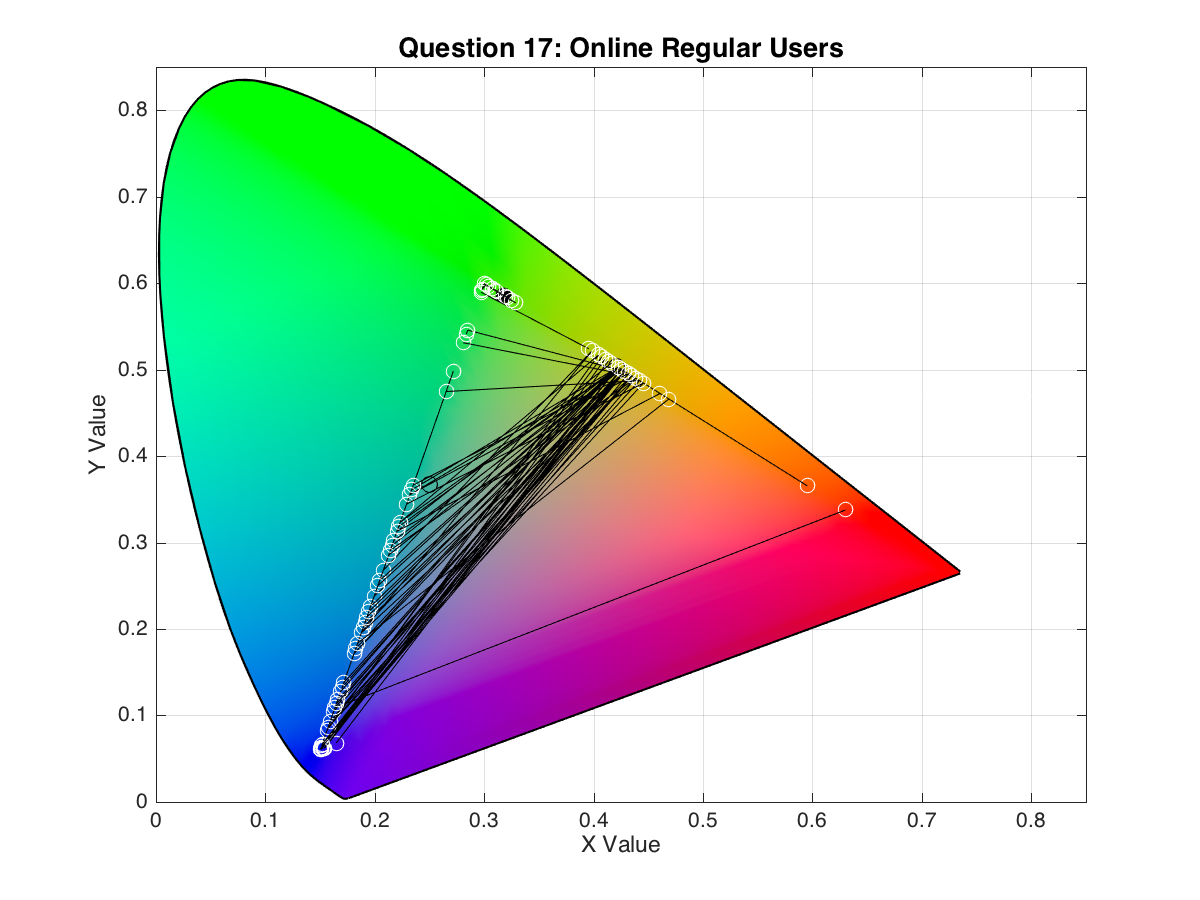
\includegraphics[width=\textwidth]{images/results/17_online_regularUsers.png}
    \caption[Online: Answers for Question 17, from regular users.]{Online: Answers for Question 17, from regular users.}
    \label{fig:greenblend_1}
  \end{minipage}\hfill
  \begin{minipage}{0.48\textwidth}
    \centering
    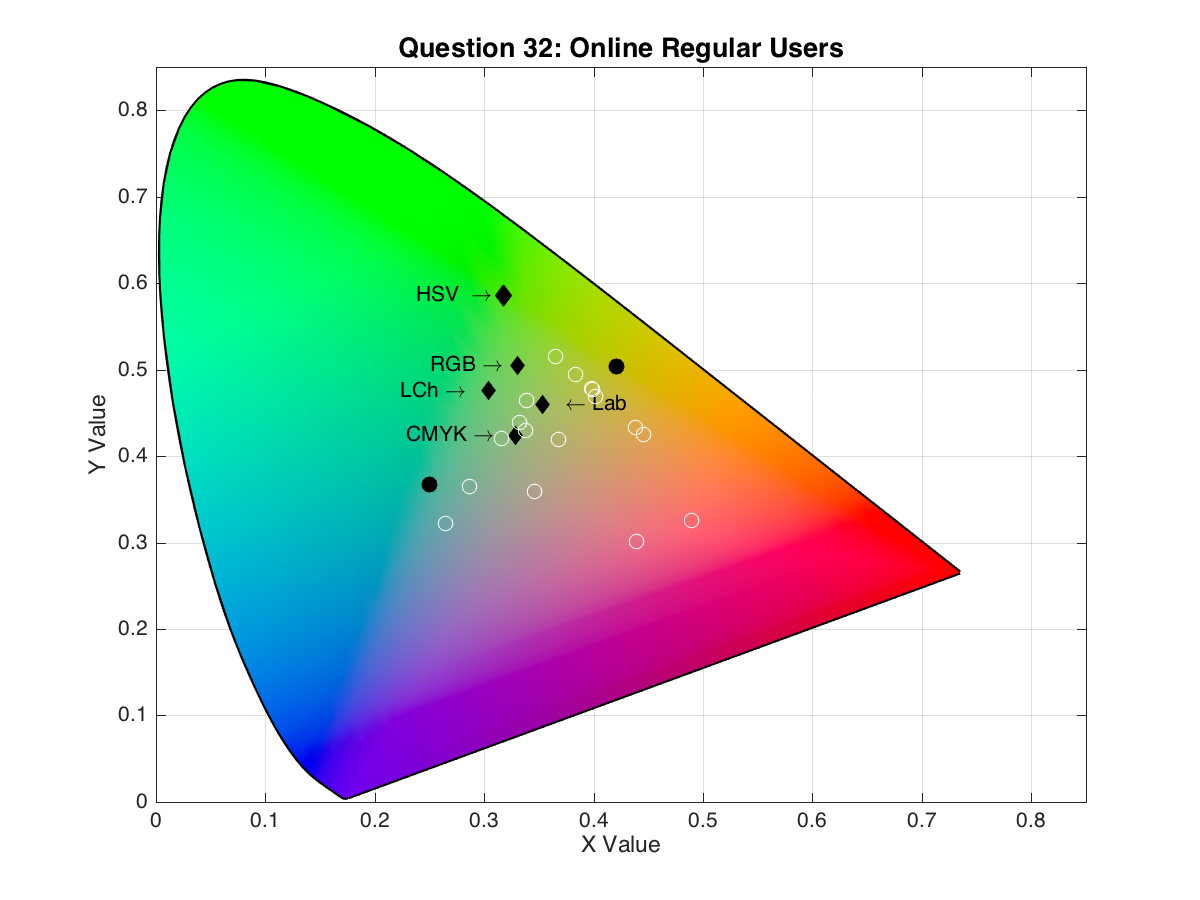
\includegraphics[width=\textwidth]{images/results/32_online_regularUsers.png}
    \caption[Online: Answers for Question 32, from regular users.]{Online: Answers for Question 32, from regular users.}
    \label{fig:greenblend_2}
  \end{minipage}
\end{figure}
%
\paragraph{\ul{Cyan + Magenta = Blue}}
%
In this question, it was expected that users indicate a mixing of Cyan and Magenta to blend in a result of Blue; these colors are primitives from the CMYK Color Model. Both the laboratory and online users provided their answers
on similar pairs, comprised between \textbf{blue shades, yellow ones, magenta's and pink, and some greens and reds}. There was also an interesting aggregation of results on both environment, near the green and yellow shades.  \\
%
However, as seen on Figures \ref{fig:blueblend_1} and \ref{fig:blueblend_2} there exists a tendency of users indicating answers very close to the given color (Blue Hue). This could reveal an \textbf{inability of detecting a blue blending
basis}, which could be related to the (lack of) descriptive power among blue colors, previously referred. \\
5
Running some descriptive statistics on top of the distance values between the given answers and the expected Cyan-Magenta Pair ($\overline{x} = 0.45$, $s = 0.11$) reveals the same high mean distance value, but a lower than previous
standard deviation of results. Due to the fact that the users indicated some answers in the magenta zone of colors and some blue/cyan hues, we could state that \textbf{although there is no strong evidence to verify this color blending, the
users show a mild ability to blend cyan and magenta, providing a blue color}. \\
%
When analyzing question number twenty-four, in which we ask the user which color is the result of blending Cyan and Magenta, we conclude that \textbf{the results, as previously happened with other primary blends, are a bit scattered}.
As before, \textbf{there is no observable tendency to begin the color blending with a particular shade of a color}. \par
%
Performing a qualitative analysis of each answer pair's colors names while comparing it to the expected pair was
\ul{Cyan-Magenta}, we obtain the following results: among 76 answers from the online users to question 7, \textbf{we conclude
that the colors Cyan and Magenta were among the least indicated ones}; instead, the users have indicated related shades to these colors,
like Blue (97 times, consistent with the previously analyzed blending using Cyan), Pink (10 times), Purple and Red with smaller repetitions.
However, it is interesting to observe that the users consistently answered a Green shade 26 times, as observed in the CIE Chromaticity Diagram
in Figure \ref{fig:blueblend_2}. The users answered 35 times with an answer pair of Blue-Blue ($46\%$ of users sample), 11 times Green-Green ($15\%$),
and 8 pairs with Blue shaded colors and Magenta derived ones ($11\%$). This is a question with poorer results, which may bye derived from aforementioned
problems related to human blue color perception.
%
\begin{figure}[!htbp]
  \centering
  \begin{minipage}{0.48\textwidth}
    \centering
    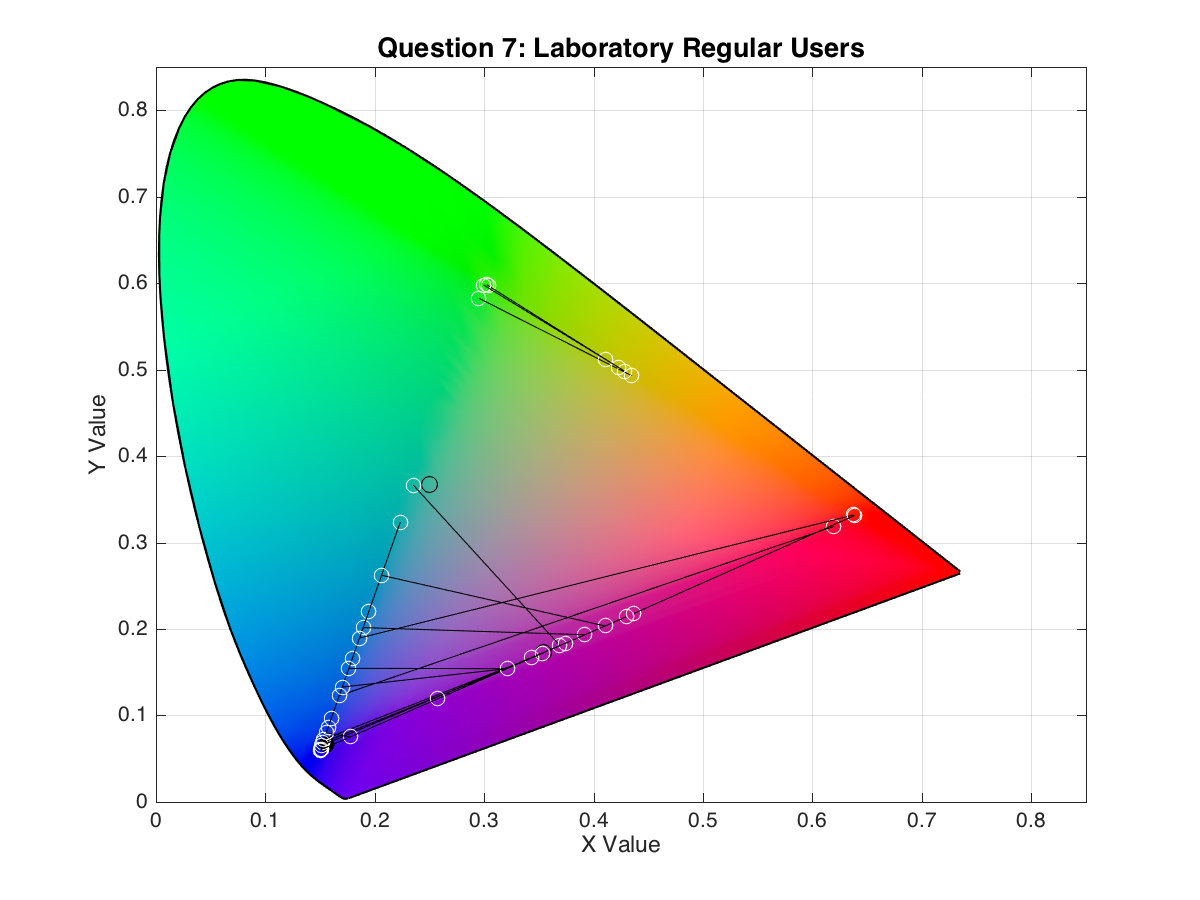
\includegraphics[width=\textwidth]{images/results/7_lab_regularUsers.png}
    \caption[Laboratory: Answers for Question 7, from regular users.]{Laboratory: Answers for Question 7, from regular users.}
    \label{fig:blueblend_1}
  \end{minipage}\hfill
  \begin{minipage}{0.48\textwidth}
    \centering
    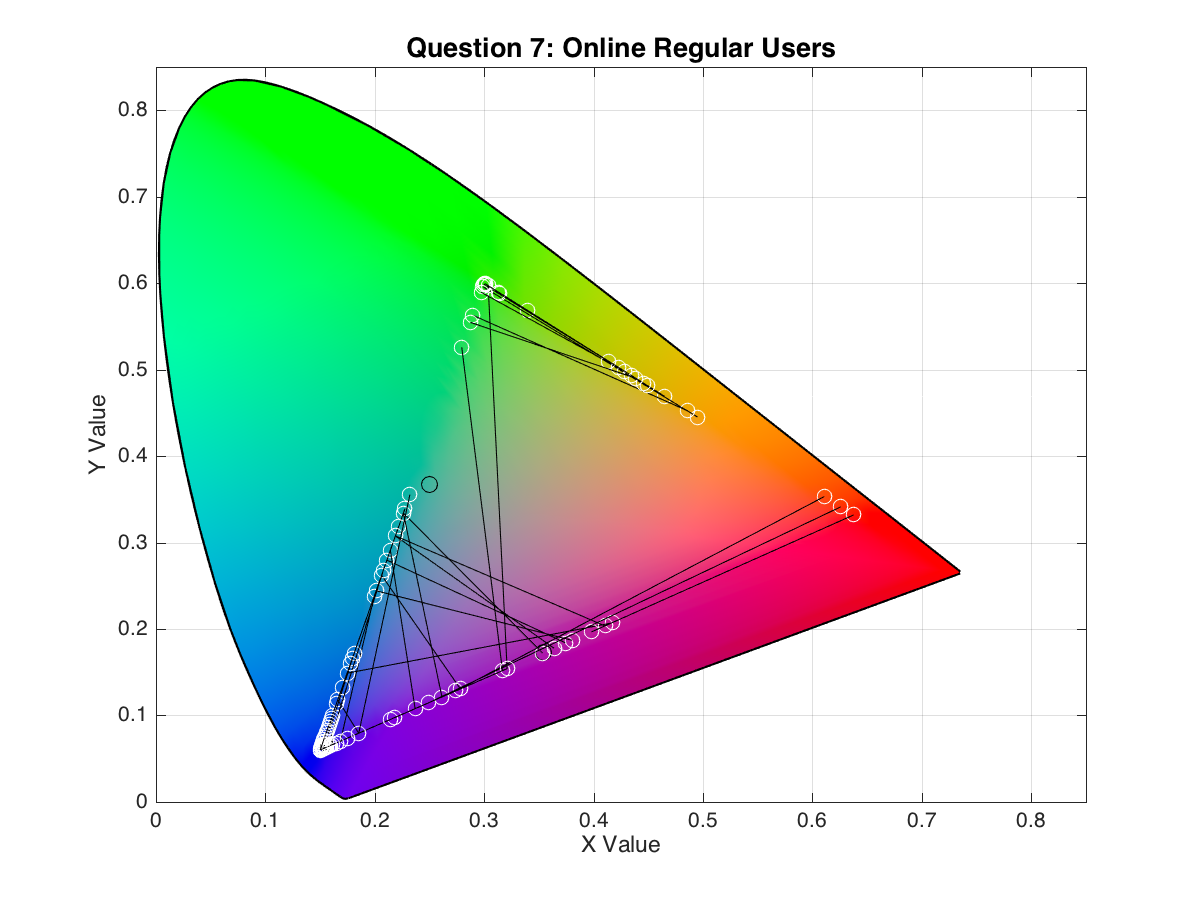
\includegraphics[width=\textwidth]{images/results/7_online_regularUsers.png}
    \caption[Online: Answers for Question 7, from regular users.]{Online: Answers for Question 7, from regular users.}
    \label{fig:blueblend_2}
  \end{minipage}
\end{figure}
%
\paragraph{\ul{Green + Blue = Cyan}}
%
As said before, this color blending was only conducted only in one way. In this question, it was expected that users indicate the result of mixing Green and Blue: Cyan; these colors are primitives from the RGB Color Model. Both the laboratory
and online users provided similar results, with an aggregation of them on the blue and cyan hues on both environment, and also in the orange hue (for unknown reasons).  \\
%
Running some descriptive statistics on top of the distance values between the given answer and the expected Cyan Color ($\overline{x} = 0.13$, $s = 0.06$) reveals some proximity to the reference pair, and a lower standard deviation of results.
Ideally, the results should be compared with the other type of question asked; since there is no question to compare and based on previous analyzed results, we can affirm that \textbf{there are mild evidences that users can detect a Green-Blue blend
to provide a Cyan color}. However, \textbf{further studies should deepen this question and determine if this affirmation could be corroborated}.
%
\paragraph{\ul{Red + Blue = Magenta}}
%
In this question, it was expected that users indicate a mixing of Red and Blue to mix in a result of Magenta. Both the laboratory and online users provided their answers on similar pairs, comprised between \textbf{blue shades, yellow ones, magenta's and
pink, and some greens and reds}. There was also an interesting aggregation of results on both environment, \textbf{along the line which unites Blue and Red}, with some scattering among the cyan and teal colors.  \\
However, as seen on Figure \ref{fig:magentablend_1} there exists a tendency of users indicating answers very close to the given color (Blue Hue). This scattering of results could be related to the \textbf{blue blending
detection problems}, previously referred. \\
%
Running some descriptive statistics on top of the distance values between the given answers and the expected Red-Blue Pair ($\overline{x} = 0.53$, $s = 0.36$) reveals the highest mean distance value so far, and also a deviation of results higher than before.
the users indicated some scattered answers in the blue zone of the chromaticity diagram: answers include Light-Blue, Sky-Blue, Navy-Blue and Cyan, besides the typical Blue; on the other hand, the users have indicated spared answers in the Magenta zone: Dark-Purple,
Pink, Magenta and Red. This shattering of data is consistent with the deviation of values obtained: we could state that \textbf{the users demonstrated some basic conception of blending red and blue to obtain magenta}. However, \textbf{the users have indicated more
detailed colors, contrary to other color blends previously evaluated}, which may have implications on the level of detail that the displaying of color should have. \\
%
Analyzing question number nineteen, in which we ask the user which color is the result of blending Red and Blue, we conclude that \textbf{the results, as previously happened with other primary blends, are a bit scattered}, leaving no plausible conclusion to formulate.
In this blending, \textbf{there is an observable tendency to begin the color blending with the red color}: on a frequency of twenty-four laboratory users, six of them ($25\%$) indicated a Red value as the first color, leaving the second color to indicate a
more detailed color; the same happens when analyzing sixty-three online users, where $33\%$ of them indicated a Red color as the first value. Relating the late dataset, it was also interesting to observe that $33\%$ of the users left the Blue color as a second answer.
This could be due to \textbf{magenta being a relatively close color to a red hue}, leading the user to indicate firstly the color which he recalls the most, that happens to be red.
%
\begin{figure}[!htbp]
  \centering
  \begin{minipage}{0.48\textwidth}
    \centering
    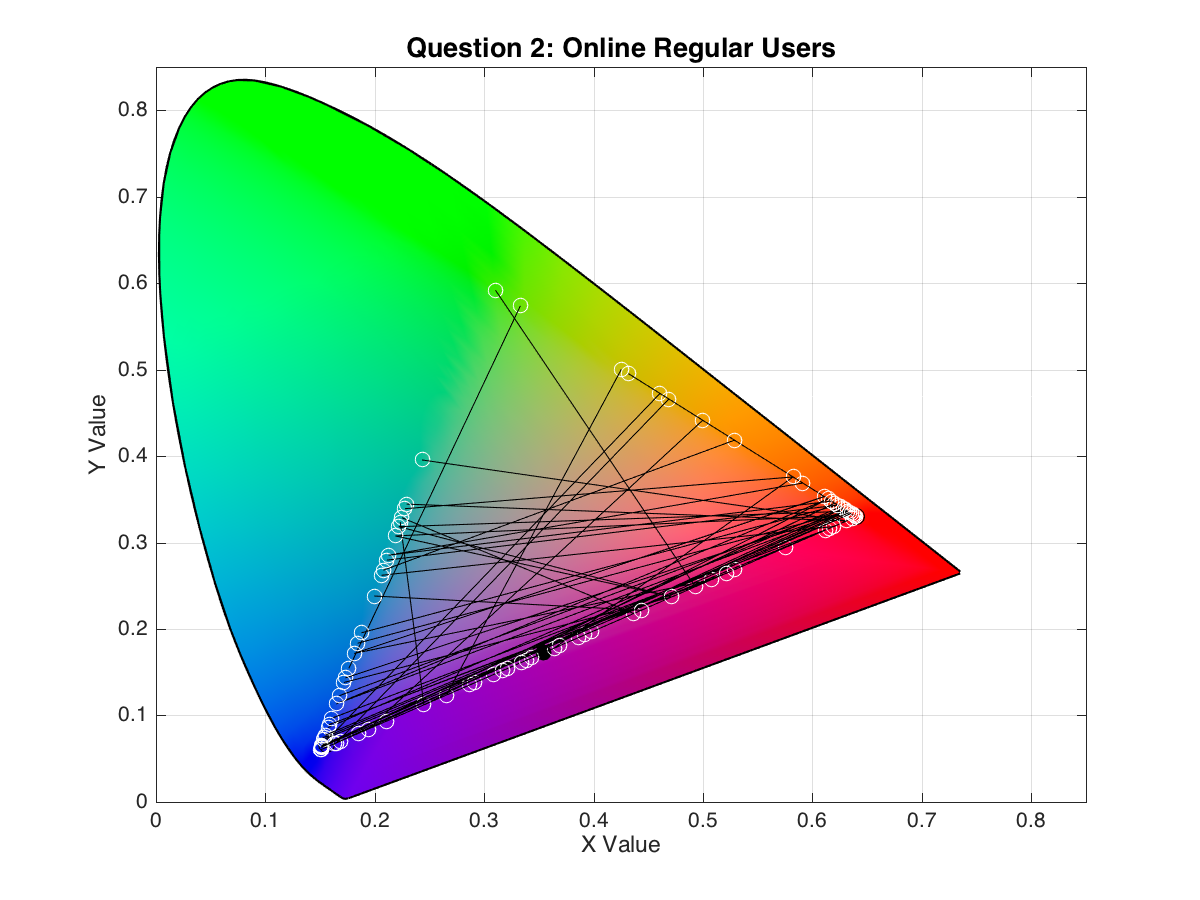
\includegraphics[width=\textwidth]{images/results/2_online_regularUsers.png}
    \caption[Online: Answers for Question 2, from regular users.]{Online: Answers for Question 2, from regular users.}
    \label{fig:magentablend_1}
  \end{minipage}\hfill
  \begin{minipage}{0.48\textwidth}
    \centering
    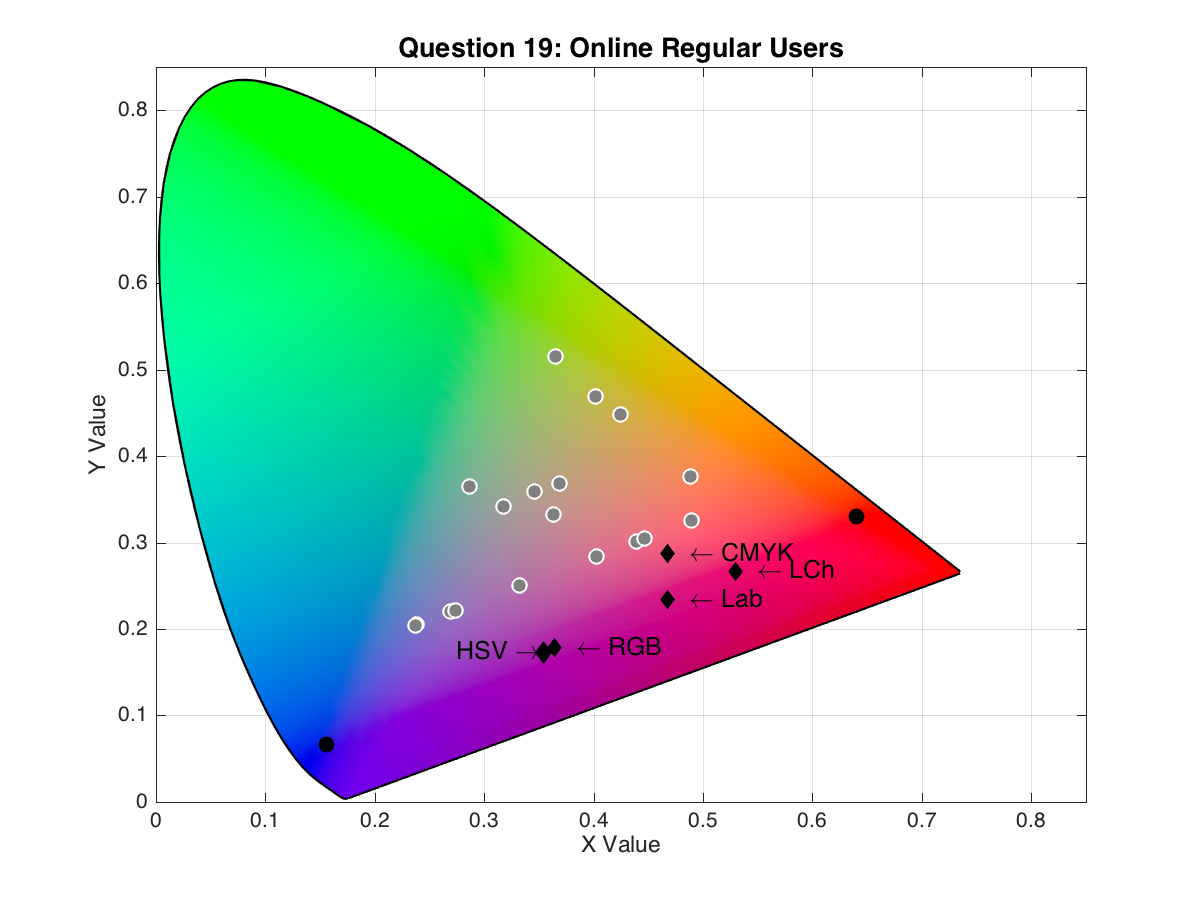
\includegraphics[width=\textwidth]{images/results/19_online_regularUsers.png}
    \caption[Online: Answers for Question 19, from regular users.]{Online: Answers for Question 19, from regular users.}
    \label{fig:magentablend_2}
  \end{minipage}
\end{figure}
%
\paragraph{\ul{Red + Green = Yellow}}
%
Lastly, it was expected that users indicate a mixing of Red and Green to mix in a result of Yellow. Both the laboratory and online users provided their answers on similar pairs, comprised between \textbf{blue shades, yellow ones, red and cyan}. There was also an
interesting aggregation of results on both environment, \textbf{along the line which unites Blue and Green, and Green and Red}, with a heavy concentration of results near the yellow shades, as seen on Figure \ref{fig:yellowblend_1}. \\
%
The answer-pairs which contained Yellow presented this colors slightly shaded to orange, which could signify that \textbf{the users provided an orangish-yellow with another color in order to blend the first one to the ideal Yellow Hue}. \\
%
Running some descriptive statistics on top of the distance ($\overline{x} = 0.41$, $s = 0.22$) reveals roughly the same mean distance and standard deviation as before. In this question, the users revealed a balmy concordance amongst themselves, according to color bins
labeling: the users centralized their answers on Blue, Navy-Blue, Orange, Red, Yellow and Green. We could state that \textbf{the users demonstrated some basic conception of blending red and green to obtain yellow}, but further studies should focus on understating which
influence is the blue color exercising on the user's mental model, since it was a constant result among study environments. \\
%
Analyzing question number eighteen, in which we ask the user which color is the result of blending Red and Green, we conclude that \textbf{the results show an approximation to the ideal color result, but a scattering over orange and yellow colors}.
In this blending, \textbf{there is a slight observable tendency to begin the color blending with a red color}, as depicted in online users' dataset ($20\%$ of fifty-three users) started the mixture with a Red Color. However, this is not a relevant result by itself: it is
indeed consistent with the result collect from the previous mixture. \\
%
Performing a qualitative analysis of each answer pair's colors names while comparing it to the expected pair was
\ul{Red-Green}, we obtain the following results: among 53 answers from the online users to question 1, \textbf{we conclude
that the colors Red and Green were among the most indicated ones}; the reference pair was indicated 15 times ($28.3\%$),
while the Green-Green pair also referred in other questions appears 25 repetitions ($47\%$): this latter pair may be referred
by the user as an "escape answer", when he does not knwo what to blend. This could be observed in Figure \ref{fig:yellowblend_1}.

instead, the users have indicated related shades to these colors,
like Blue (97 times, consistent with the previously analyzed blending using Cyan), Pink (10 times), Purple and Red with smaller repetitions.
However, it is interesting to observe that the users consistently answered a Green shade 26 times, as observed in the CIE Chromaticity Diagram
in Figure \ref{fig:blueblend_2}. The users answered 35 times with an answer pair of Blue-Blue ($46\%$ of users sample), 11 times Green-Green ($15\%$),
and 8 pairs with Blue shaded colors and Magenta derived ones ($11\%$). This is a question with poorer results, which may bye derived from aforementioned
problems related to human blue color perception.
%
\begin{figure}[!htbp]
  \centering
  \begin{minipage}{0.48\textwidth}
    \centering
    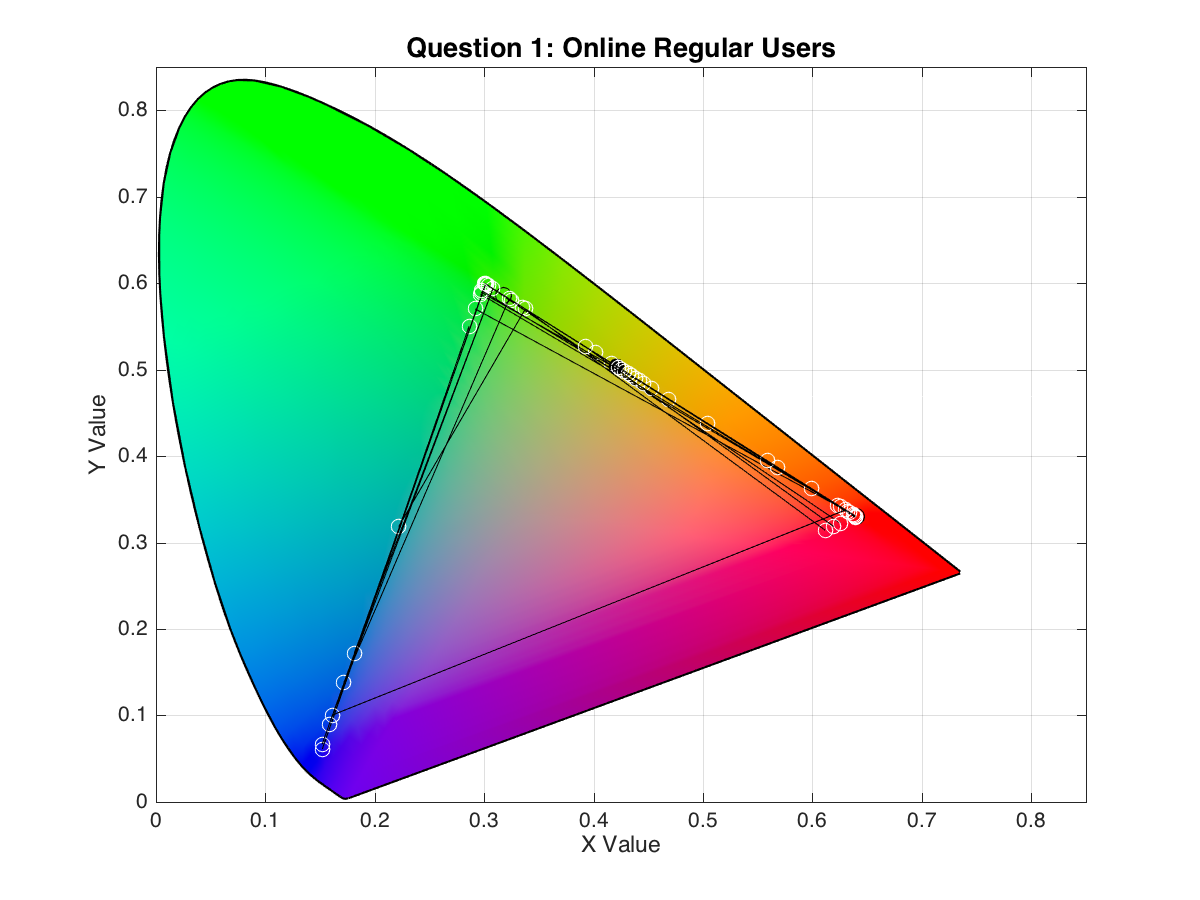
\includegraphics[width=\textwidth]{images/results/1_online_regularUsers.png}
    \caption[Online: Answers for Question 1, from regular users.]{Online: Answers for Question 1, from regular users.}
    \label{fig:yellowblend_1}
  \end{minipage}\hfill
  \begin{minipage}{0.48\textwidth}
    \centering
    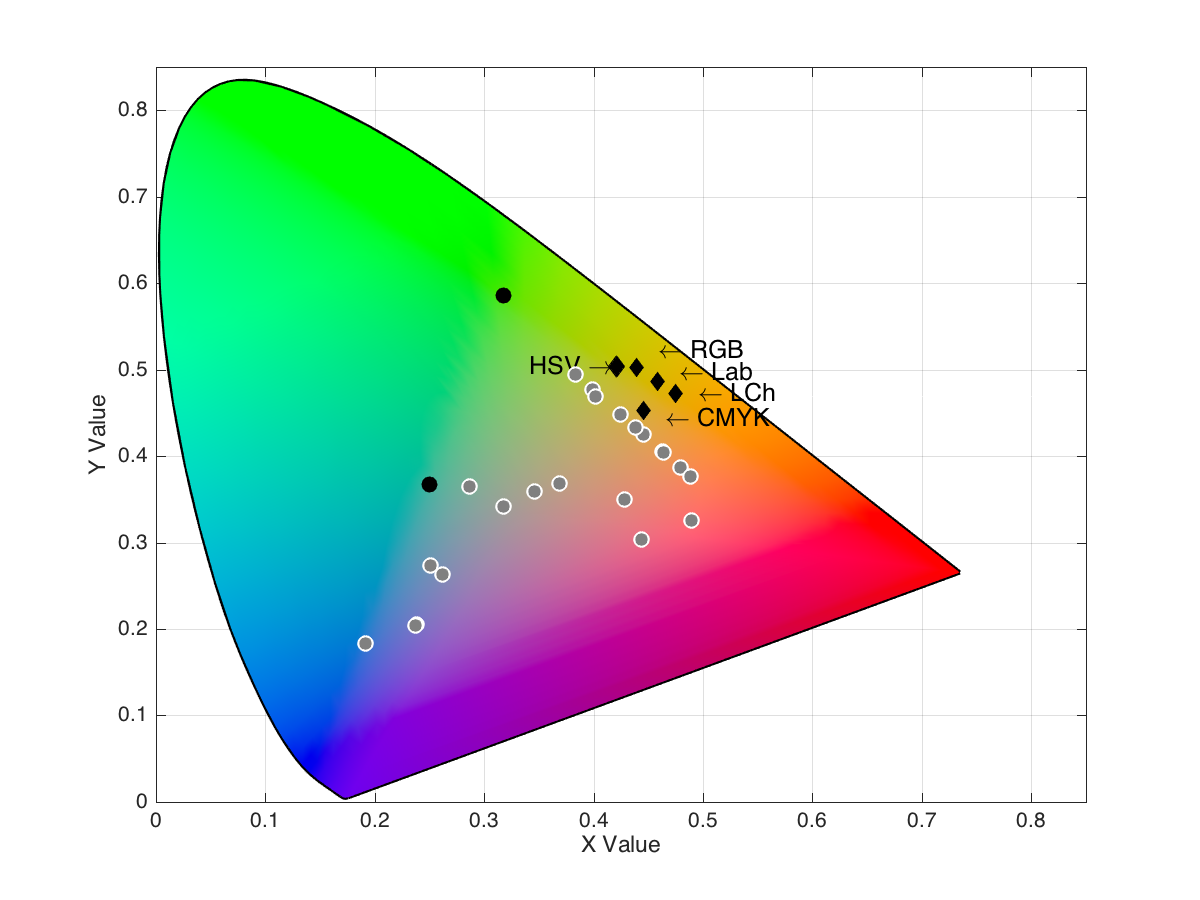
\includegraphics[width=\textwidth]{images/results/18_online_regularUsers.png}
    \caption[Online: Answers for Question 18, from regular users.]{Online: Answers for Question 18, from regular users.}
    \label{fig:yellowblend_2}
  \end{minipage}
\end{figure}
%
\subsubsection{Color Blending Effort}
\label{subsubsec:difficulty_rating}
%
We have collected from the users the easiness of blending two shades of colors, when concluding each answer. This easiness is reflected in an numerical scale, ranged from one to five, being one the hardest level of effort, and five the easiest level
of effort. The results were gathered and analyzed, and are resumed in Table \ref{table:difficulties_blendings}, where we associate to each color blending the effort degrees the users found when answering the two types of questions discussed before.
For better appreciation, the table presents in green shaded cells the color blendings which have a $Mo$ value of Difficulty level equal to five, and shaded in red the color blendings which present the lowest $Mo$ value (two). \par
%
\begin{table}[htbp]
  \resizebox{\textwidth}{!} {
  \begin{tabular}{@{}ccclcccccccccccc@{}}
    \toprule
    \multicolumn{2}{c}{}                                                     & \multicolumn{2}{c}{}                                       & \multicolumn{6}{c}{Given the Result, Asked for Basis}                                                                                                                                                                               & \multicolumn{6}{c}{Given the Basis, Asked for the Result}                                                                                                                                                                                                                                                                   \\ \cmidrule(l){5-16}
    \multicolumn{2}{c}{\multirow{-2}{*}{Blending Basis}}                     & \multicolumn{2}{c}{\multirow{-2}{*}{Blending Result}}      & \multicolumn{3}{c}{Laboratory}                                                                                   & \multicolumn{3}{c}{Online}                                                                                       & \multicolumn{3}{c}{Laboratory}                                                                                                                      & \multicolumn{3}{c}{Online}                                                                                                                                            \\ \midrule
    C1                      & C2                                             & \multicolumn{2}{c|}{C3}                                    & Mean ($\overline{x}$)        & Std-Dev ($s$)         & Mode ($Mo$)                                             & Mean ($\overline{x}$)        & Std-Dev ($s$)         & \multicolumn{1}{c|}{Mode ($Mo$)}                        & Mean ($\overline{x}$)                          & Std-Dev ($s$)                          & Mode ($Mo$)                                             & Mean ($\overline{x}$)                          & Std-Dev ($s$)                          & \multicolumn{1}{c|}{Mode ($Mo$)}                                          \\ \midrule
    Red                     & \multicolumn{1}{c|}{Green}                     & \multicolumn{2}{c|}{\cellcolor[HTML]{FFFF00}(77, 93, 14)}  & \multicolumn{1}{c|}{3.58} & \multicolumn{1}{c|}{1.21}  & \multicolumn{1}{c|}{\cellcolor[HTML]{32CB00}\textbf{5}} & \multicolumn{1}{c|}{3.72} & \multicolumn{1}{c|}{1.45}  & \multicolumn{1}{c||}{\cellcolor[HTML]{32CB00}\textbf{5}} & \multicolumn{1}{c|}{3.10}                   & \multicolumn{1}{c|}{1.05}                   & \multicolumn{1}{c|}{3}                                  & \multicolumn{1}{c|}{2.67}                   & \multicolumn{1}{c|}{1.20}                   & \multicolumn{1}{c|}{3}                                                    \\ \midrule
    Red                     & \multicolumn{1}{c|}{Blue}                      & \multicolumn{2}{c|}{\cellcolor[HTML]{FF00FF}(59, 28, 97)}  & \multicolumn{1}{c|}{3.13} & \multicolumn{1}{c|}{1.41}  & \multicolumn{1}{c|}{3}                                  & \multicolumn{1}{c|}{3.17} & \multicolumn{1}{c|}{1.26}  & \multicolumn{1}{c||}{3}                                  & \multicolumn{1}{c|}{3.54}                   & \multicolumn{1}{c|}{0.96}                   & \multicolumn{1}{c|}{3}                                  & \multicolumn{1}{c|}{3.57}                   & \multicolumn{1}{c|}{1.23}                   & \multicolumn{1}{c|}{\cellcolor[HTML]{32CB00}\textbf{5}}                   \\ \midrule
    Green                   & \multicolumn{1}{c|}{Blue}                      & \multicolumn{2}{c|}{\cellcolor[HTML]{00FFFF}(54, 79, 107)} & \multicolumn{6}{c||}{-}                                                                                                                                                                                                              & \multicolumn{1}{c|}{3.32}                   & \multicolumn{1}{c|}{1.22}                   & \multicolumn{1}{c|}{\cellcolor[HTML]{FD6864}\textbf{2}} & \multicolumn{1}{c|}{3.10}                   & \multicolumn{1}{c|}{1.25}                   & \multicolumn{1}{c|}{3}                                                    \\ \midrule
                            & \multicolumn{1}{c|}{}                          & \multicolumn{2}{c|}{\cellcolor[HTML]{80FF00}(45, 76, 12)}  & \multicolumn{1}{c|}{3.95} & \multicolumn{1}{c|}{1.09}  & \multicolumn{1}{c|}{4}                                  & \multicolumn{1}{c|}{3.80} & \multicolumn{1}{c|}{1.05}  & \multicolumn{1}{c||}{3}                                  & \multicolumn{1}{c|}{}                       & \multicolumn{1}{c|}{}                       & \multicolumn{1}{c|}{}                                   & \multicolumn{1}{c|}{}                       & \multicolumn{1}{c|}{}                       & \multicolumn{1}{c|}{}                                                     \\ \cmidrule(lr){3-10}
    \multirow{-2}{*}{Red}   & \multicolumn{1}{c|}{\multirow{-2}{*}{Cyan}}    & \multicolumn{2}{c|}{\cellcolor[HTML]{7F00FF}(27, 12, 95)}  & \multicolumn{1}{c|}{3.28} & \multicolumn{1}{c|}{0.97}  & \multicolumn{1}{c|}{3}                                  & \multicolumn{1}{c|}{3.49} & \multicolumn{1}{c|}{1.15}  & \multicolumn{1}{c||}{4}                                  & \multicolumn{1}{c|}{\multirow{-2}{*}{3.14}} & \multicolumn{1}{c|}{\multirow{-2}{*}{1.06}} & \multicolumn{1}{c|}{\multirow{-2}{*}{3}}                & \multicolumn{1}{c|}{\multirow{-2}{*}{2.97}} & \multicolumn{1}{c|}{\multirow{-2}{*}{1.11}} & \multicolumn{1}{c|}{\multirow{-2}{*}{3}}                                  \\ \midrule
    Red                     & \multicolumn{1}{c|}{Magenta}                   & \multicolumn{2}{c|}{\cellcolor[HTML]{FF0080}(45, 23, 22)}  & \multicolumn{1}{c|}{3.22} & \multicolumn{1}{c|}{0.81}  & \multicolumn{1}{c|}{3}                                  & \multicolumn{1}{c|}{3.13} & \multicolumn{1}{c|}{1.19}  & \multicolumn{1}{c||}{3}                                  & \multicolumn{1}{c|}{3.14}                   & \multicolumn{1}{c|}{0.89}                   & \multicolumn{1}{c|}{3}                                  & \multicolumn{1}{c|}{3.10}                   & \multicolumn{1}{c|}{1.08}                   & \multicolumn{1}{c|}{3}                                                    \\ \midrule
    Red                     & \multicolumn{1}{c|}{Yellow}                    & \multicolumn{2}{c|}{\cellcolor[HTML]{FF8000}(49, 37, 5)}   & \multicolumn{1}{c|}{3.86} & \multicolumn{1}{c|}{1.08}  & \multicolumn{1}{c|}{4}                                  & \multicolumn{1}{c|}{4.08} & \multicolumn{1}{c|}{1.00}  & \multicolumn{1}{c||}{\cellcolor[HTML]{32CB00}\textbf{5}} & \multicolumn{1}{c|}{3.26}                   & \multicolumn{1}{c|}{1.06}                   & \multicolumn{1}{c|}{3}                                  & \multicolumn{1}{c|}{4.10}                   & \multicolumn{1}{c|}{1.05}                   & \multicolumn{1}{c|}{\cellcolor[HTML]{32CB00}\textbf{5}}                   \\ \midrule
    Cyan                    & \multicolumn{1}{c|}{Magenta}                   & \multicolumn{2}{c|}{\cellcolor[HTML]{0000FF}(18, 7, 95)}   & \multicolumn{1}{c|}{3.5}  & \multicolumn{1}{c|}{1.19}  & \multicolumn{1}{c|}{3}                                  & \multicolumn{1}{c|}{3.32} & \multicolumn{1}{c|}{1.59}  & \multicolumn{1}{c||}{\cellcolor[HTML]{32CB00}\textbf{5}} & \multicolumn{1}{c|}{3.04}                   & \multicolumn{1}{c|}{1.23}                   & \multicolumn{1}{c|}{\cellcolor[HTML]{FD6864}\textbf{2}} & \multicolumn{1}{c|}{2.90}                   & \multicolumn{1}{c|}{1.23}                   & \multicolumn{1}{c|}{3}                                                    \\ \midrule
    Magenta                 & \multicolumn{1}{c|}{Yellow}                    & \multicolumn{2}{c|}{\cellcolor[HTML]{FF0000}(41, 21, 2)}   & \multicolumn{1}{c|}{2.92} & \multicolumn{1}{c|}{1.22}  & \multicolumn{1}{c|}{\cellcolor[HTML]{FD6864}\textbf{2}} & \multicolumn{1}{c|}{2.62} & \multicolumn{1}{c|}{1.50}  & \multicolumn{1}{c||}{\cellcolor[HTML]{32CB00}\textbf{5}} & \multicolumn{1}{c|}{2.70}                   & \multicolumn{1}{c|}{0.82}                   & \multicolumn{1}{c|}{3}                                  & \multicolumn{1}{c|}{2.75}                   & \multicolumn{1}{c|}{1.24}                   & \multicolumn{1}{c|}{\cellcolor[HTML]{FD6864}\textbf{2}}                   \\ \midrule
    Green                   & \multicolumn{1}{c|}{Cyan}                      & \multicolumn{2}{c|}{\cellcolor[HTML]{00FF80}(40, 73, 32)}  & \multicolumn{1}{c|}{3.42} & \multicolumn{1}{c|}{0.90}  & \multicolumn{1}{c|}{3}                                  & \multicolumn{1}{c|}{3.26} & \multicolumn{1}{c|}{1.10}  & \multicolumn{1}{c||}{4}                                  & \multicolumn{1}{c|}{3.50}                   & \multicolumn{1}{c|}{1.20}                   & \multicolumn{1}{c|}{4}                                  & \multicolumn{1}{c|}{2.94}                   & \multicolumn{1}{c|}{1.19}                   & \multicolumn{1}{c|}{\cellcolor[HTML]{FD6864}\textbf{2}}                   \\ \midrule
                            & \multicolumn{1}{c|}{}                          & \multicolumn{2}{c|}{\cellcolor[HTML]{0080FF}(26, 23, 98)}  & \multicolumn{1}{c|}{3.43} & \multicolumn{1}{c|}{1.16}  & \multicolumn{1}{c|}{3}                                  & \multicolumn{1}{c|}{3.50} & \multicolumn{1}{c|}{1.35}  & \multicolumn{1}{c||}{3}                                  & \multicolumn{1}{c|}{}                       & \multicolumn{1}{c|}{}                       & \multicolumn{1}{c|}{}                                   & \multicolumn{1}{c|}{}                       & \multicolumn{1}{c|}{}                       & \multicolumn{1}{c|}{\cellcolor[HTML]{FD6864}}                             \\ \cmidrule(lr){3-10}
    \multirow{-2}{*}{Green} & \multicolumn{1}{c|}{\multirow{-2}{*}{Magenta}} & \multicolumn{2}{c|}{\cellcolor[HTML]{FF8000}(49, 37, 5)}   & \multicolumn{1}{c|}{4.17} & \multicolumn{1}{c|}{0.887} & \multicolumn{1}{c|}{\cellcolor[HTML]{32CB00}\textbf{5}} & \multicolumn{1}{c|}{2.06} & \multicolumn{1}{c|}{1.035} & \multicolumn{1}{c||}{\cellcolor[HTML]{32CB00}\textbf{5}} & \multicolumn{1}{c|}{\multirow{-2}{*}{2.68}} & \multicolumn{1}{c|}{\multirow{-2}{*}{1.16}} & \multicolumn{1}{c|}{\multirow{-2}{*}{3}}                & \multicolumn{1}{c|}{\multirow{-2}{*}{2.25}} & \multicolumn{1}{c|}{\multirow{-2}{*}{1.17}} & \multicolumn{1}{c|}{\multirow{-2}{*}{\cellcolor[HTML]{FD6864}\textbf{2}}} \\ \midrule
    Green                   & \multicolumn{1}{c|}{Yellow}                    & \multicolumn{2}{c|}{\cellcolor[HTML]{80FF00}(45, 76, 12)}  & \multicolumn{1}{c|}{3.71} & \multicolumn{1}{c|}{0.96}  & \multicolumn{1}{c|}{3}                                  & \multicolumn{1}{c|}{3.67} & \multicolumn{1}{c|}{1.07}  & \multicolumn{1}{c||}{4}                                  & \multicolumn{1}{c|}{3.18}                   & \multicolumn{1}{c|}{1.19}                   & \multicolumn{1}{c|}{3}                                  & \multicolumn{1}{c|}{3.31}                   & \multicolumn{1}{c|}{1.24}                   & \multicolumn{1}{c|}{4}                                                    \\ \midrule
    Blue                    & \multicolumn{1}{c|}{Cyan}                      & \multicolumn{2}{c|}{\cellcolor[HTML]{0080FF}(26, 23, 98)}  & \multicolumn{1}{c|}{3.63} & \multicolumn{1}{c|}{1.26}  & \multicolumn{1}{c|}{\cellcolor[HTML]{32CB00}\textbf{5}} & \multicolumn{1}{c|}{3.53} & \multicolumn{1}{c|}{1.12}  & \multicolumn{1}{c||}{4}                                  & \multicolumn{1}{c|}{3.48}                   & \multicolumn{1}{c|}{0.99}                   & \multicolumn{1}{c|}{3}                                  & \multicolumn{1}{c|}{3.41}                   & \multicolumn{1}{c|}{1.12}                   & \multicolumn{1}{c|}{3}                                                    \\ \midrule
    Blue                    & \multicolumn{1}{c|}{Magenta}                   & \multicolumn{2}{c|}{\cellcolor[HTML]{8000FF}(27, 12, 95)}  & \multicolumn{1}{c|}{3.50} & \multicolumn{1}{c|}{0.8}   & \multicolumn{1}{c|}{3}                                  & \multicolumn{1}{c|}{3.49} & \multicolumn{1}{c|}{1.13}  & \multicolumn{1}{c||}{3}                                  & \multicolumn{1}{c|}{3.25}                   & \multicolumn{1}{c|}{1.11}                   & \multicolumn{1}{c|}{4}                                  & \multicolumn{1}{c|}{3.19}                   & \multicolumn{1}{c|}{1.16}                   & \multicolumn{1}{c|}{3}                                                    \\ \midrule
                            & \multicolumn{1}{c|}{}                          & \multicolumn{2}{c|}{\cellcolor[HTML]{00FF80}(40, 73, 32)}  & \multicolumn{1}{c|}{3.75} & \multicolumn{1}{c|}{0.86}  & \multicolumn{1}{c|}{4}                                  & \multicolumn{1}{c|}{3.58} & \multicolumn{1}{c|}{1.14}  & \multicolumn{1}{c||}{4}                                  & \multicolumn{1}{c|}{}                       & \multicolumn{1}{c|}{}                       & \multicolumn{1}{c|}{}                                   & \multicolumn{1}{c|}{}                       & \multicolumn{1}{c|}{}                       & \multicolumn{1}{c|}{}                                                     \\ \cmidrule(lr){3-10}
    \multirow{-2}{*}{Blue}  & \multicolumn{1}{c|}{\multirow{-2}{*}{Yellow}}  & \multicolumn{2}{c|}{\cellcolor[HTML]{FF007F}(45, 23, 22)}  & \multicolumn{1}{c|}{3.47} & \multicolumn{1}{c|}{0.83}  & \multicolumn{1}{c|}{3}                                  & \multicolumn{1}{c|}{3.27} & \multicolumn{1}{c|}{1.17}  & \multicolumn{1}{c||}{3}                                  & \multicolumn{1}{c|}{\multirow{-2}{*}{3.57}} & \multicolumn{1}{c|}{\multirow{-2}{*}{1.03}} & \multicolumn{1}{c|}{\multirow{-2}{*}{4}}                & \multicolumn{1}{c|}{\multirow{-2}{*}{3.61}} & \multicolumn{1}{c|}{\multirow{-2}{*}{1.12}} & \multicolumn{1}{c|}{\multirow{-2}{*}{3}}                                  \\ \midrule
    Cyan                    & \multicolumn{1}{c|}{Yellow}                    & \multicolumn{2}{c|}{\cellcolor[HTML]{00FF00}(36, 72, 13)}  & \multicolumn{1}{c|}{3.96} & \multicolumn{1}{c|}{0.98}  & \multicolumn{1}{c|}{4}                                  & \multicolumn{1}{c|}{3.90} & \multicolumn{1}{c|}{1.16}  & \multicolumn{1}{c||}{\cellcolor[HTML]{32CB00}\textbf{5}} & \multicolumn{1}{c|}{3.36}                   & \multicolumn{1}{c|}{0.95}                   & \multicolumn{1}{c|}{4}                                  & \multicolumn{1}{c|}{3.54}                   & \multicolumn{1}{c|}{1.17}                   & \multicolumn{1}{c|}{3}                                                    \\ \bottomrule
  \end{tabular}}
  \caption[Color Blending Effort, according to users' answers.]{Color Blending Effort, according to users' answers.}
  \label{table:difficulties_blendings}
\end{table}
%
As seen on the table, the results are in agreement with the ones collected and concluded before: the \textbf{blending of Red-Green resulting in Yellow}, \textbf{blending of Red-Yellow and Green-Magenta, both resulting in Orange} and the
\textbf{blending of Cyan-Yellow resulting in Green} were the mixtures which, according to the users' answers, had the lowest effort of blending, consequently the highest rating of easiness; particularly for the mixture of Red and Yellow, resulting in
Orange, it provides the best results in both question types. Contrary, the questions which had the lowest results were almost always the ones in which the user was inquired about the result of given blending basis. \par
%
Nevertheless, it is interesting to observe that the results for the generality of questions encircle the rating of 2 and 3 in the interval $[1 ; 5]$, which could indicate that \textbf{apart from the obvious color blendings which proved to yield the
best results, all the other blendings show nor an easy or hard level of effort to mix the basis}. These results are confirmed by the online responses, by running a Friedman Test which indicates us that there are no statistically significant differences
($p < 0.05$) when comparing the results from the laboratory environment, with the online results. \par
%
During the analysis and data cleaning, we have found a substantial portion of data which reflected the users' answers which contained only one component, when it was expected a pair of two. These answers were separated from the original dataset and we
have decided not to eliminate these answers, since they could provide useful inputs to our analysis, discerning if the users did not indicate a second color for the sake of convenience, or because they did not know what to blend, or simply to blend the given
answer with a white color, lightning it down to a lighter color. The blendings which had more solitary answer were \textbf{Green-Magenta, producing a Blue shade} (\ul{63 entries}), \textbf{Red-Green, producing Yellow} (\ul{60 entries}) and
\textbf{Blue-Yellow, producing a Pink shade} (56 entries); the ones which had less were \textbf{Red-Yellow, producing a Orange shade} (26 entries), \textbf{Green-Yellow, producing a Lime-Green color} (24 entries) and \textbf{Blue-Magenta,
producing a Purple shade} (20 entries). Analyzing these answers, we conclude that the option of \textbf{indicating only one color \ul{is not} due to knowing just one primitive of the blending}, since a barely set of users indicated correctly one primitive.
However, there was a tendency for users to indicate colors which were near ($distance < 0.1$) the resulting color (already presented): this could indicate that \textbf{the users either left an empty color as a whitening one, along with a darker shade than the
result, or they indicated the same color as the result, according to their expectation and color perception}. Since it is not possible for us to judge this information based on these results only, it would be ideal if further studies could deepen this matter.
Figures \ref{fig:white_2} and \ref{fig:white_3} all represent the set of answer-pairs with one white component, for questions one, ten and fifteen, respectively. \par
%
\begin{figure}[!htbp]
  \centering
  \begin{minipage}{0.48\textwidth}
    \centering
    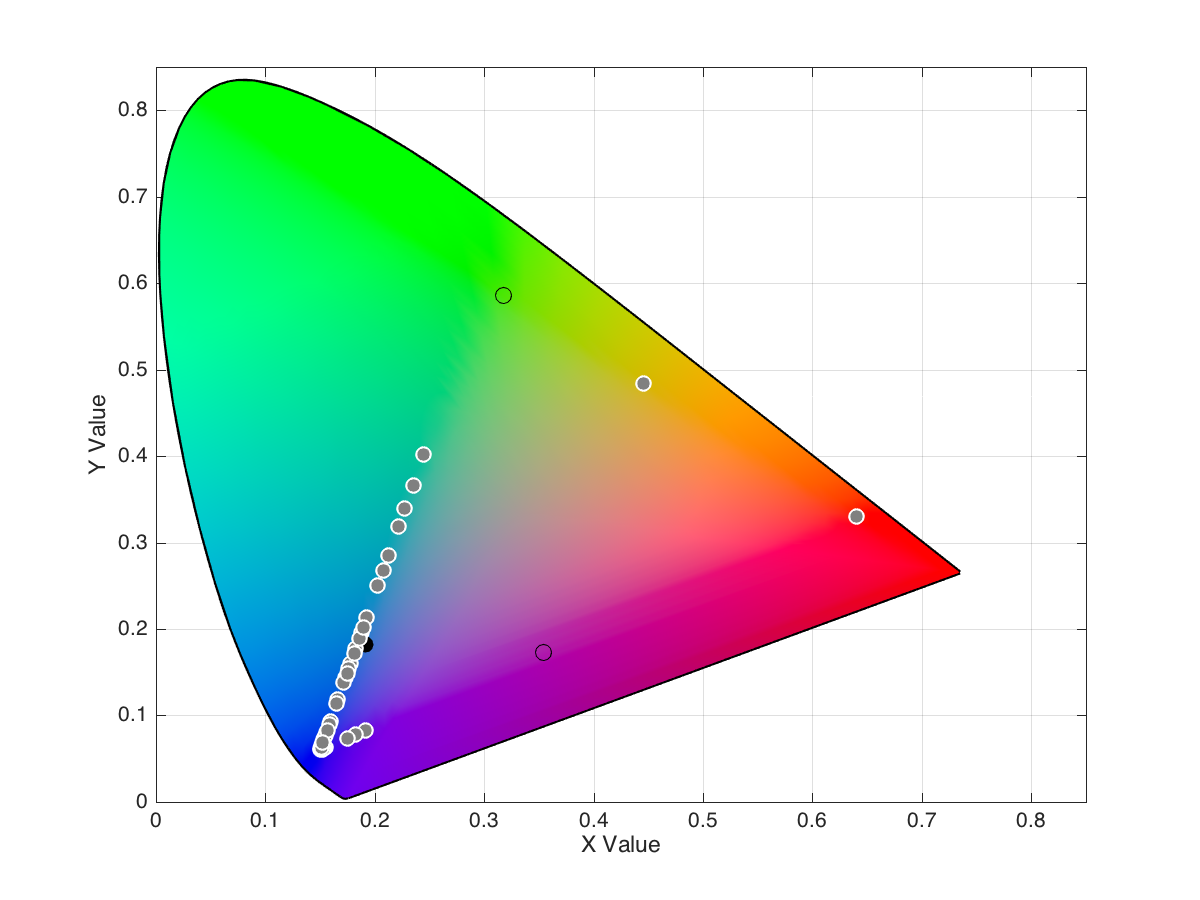
\includegraphics[width=\textwidth]{images/results/10_white_answers.png}
    \caption[Answer-pairs with one white component, from Question 10.]{Answer-pairs with one white component, from Question 10.}
    \label{fig:white_2}
  \end{minipage}\hfill
  \begin{minipage}{0.48\textwidth}
    \centering
    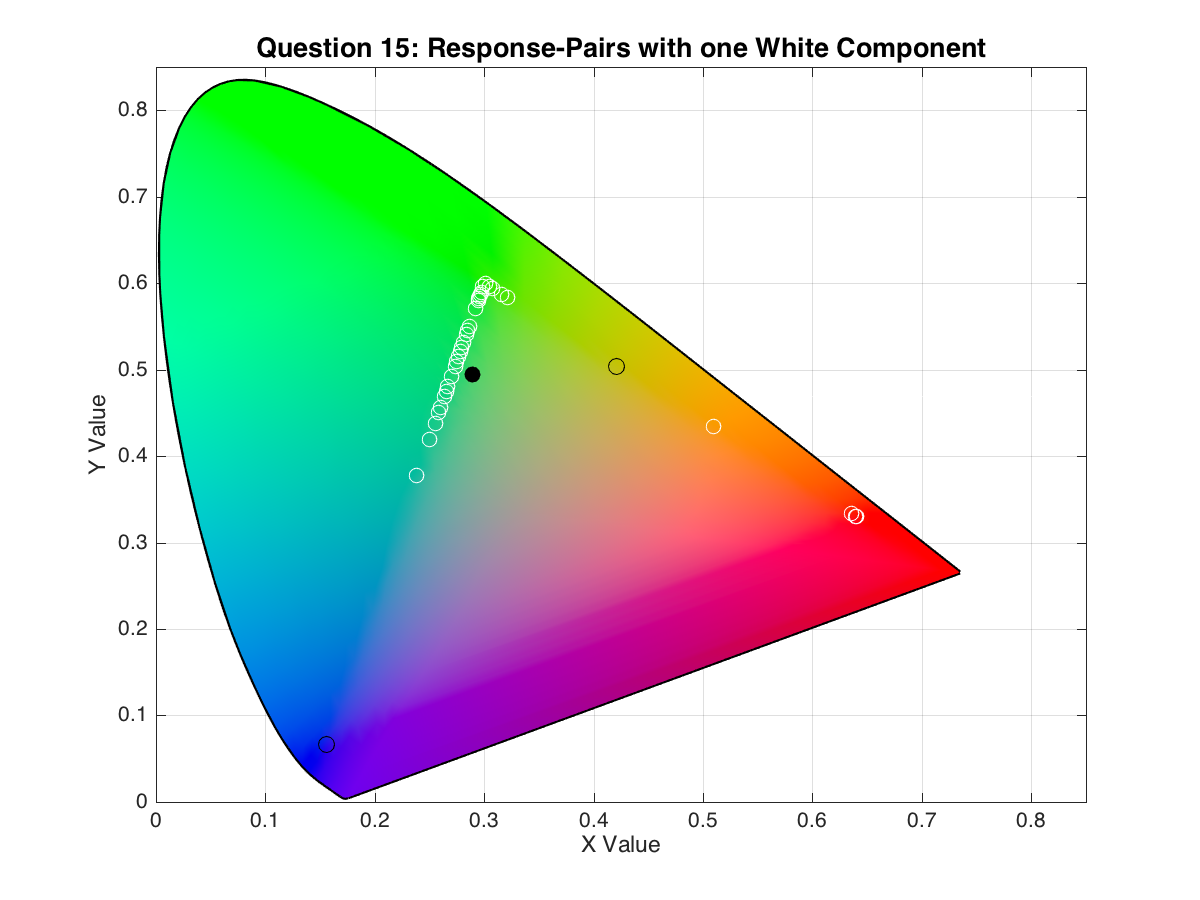
\includegraphics[width=\textwidth]{images/results/15_white_answers.png}
    \caption[Answer-pairs with one white component, from Question 15.]{Answer-pairs with one white component, from Question 15.}
    \label{fig:white_3}
  \end{minipage}
\end{figure}
%
\subsection{Demographic Results}
\label{subsec:results_demographic}
%
To conclude the analysis of our dataset, we performed a set of statistic tests to realize if there is some kind of connection between the demographic information of our users and the answers given by them, for example a relation between the answers given by
the male and female users, or even if the younger users interpret the color blendings differently from the older ones. As referred in the beginning of this Section, we have separated the users among some demographic groups: regarding the age division we have
created six groups (users aged below 20 years, aged between 20 and 29, between 30 and 39, 40 and 49, 50 and 59, and above 60 years), and for the gender we have divided the dataset according to female, male and other gendered users. These groups were, then, iterated
by question, performing a \ul{Spearman's Rank-Order Correlation test} between the ages and genders, with the answers; since the amount of data available is quite high, this test would dictate which questions would be subject of further analysis in this Section. \par
%
Additionally, it would be interesting to perform a crossed analysis between genders and age groups: however, the size of the dataset does not provide the amount of information needed to corroborate such analysis. Hereupon, we are going to divide the analysis of these demographic
groups on the next subSections, starting by analyzing the results for the age groups highlighting the questions which manifested statistically significant correlations, followed by the evaluation of the gender groups. To end this Section, we will perform an additional
informal evaluation of the results collected from color vision deficient users.
%
\subsubsection{Age Groups}
\label{subsubsec:demo_age}
%
Recalling Table \ref{table:profiling_genderacademic}, present of Section \ref{subsec:results_userprofile}, we have collected a total of 259 users, being \ul{38 users aged below 20 years}, \ul{162 users aged between 20 and 29 years}, \ul{20 users aged between 30 and 39 years},
\ul{19 users aged between 40 and 49 years}, \ul{12 users aged between 50 and 59 years} and \ul{8 users aged above 60 years}. When analyzing the results from all 32 questions, for each of these age groups, with Spearman's Correlation test we conclude that there are no statistically
significant correlations ($\rho < 0.05$) when comparing the distances from answers blended in each color model (HSV, CIE-L*C*h*, CMYK, RGB and CIE-L*a*b*) with the age from the users, for the majority of questions except for a small subset: from all 32 questions asked, seven of them presented weak,
positive and negative correlation between the age values and the calculated distances, which have statistically significant correlation values ($\rho < 0.05$). \par
%
These questions are \ul{number six} ($r_s(6) = 0.22$, $\rho = 0.013$), \ul{seven} ($r_s(7) = -0.18$, $\rho = 0.032$), \ul{eight} ($r_s(8) = -0.21$, $\rho = 0.015$), \ul{nine} ($r_s(9) = 0.19$, $\rho = 0.029$), \ul{nineteen} ($r_s(19) = 0.19, \rho = 0.028$), \ul{twenty-five}
($r_s(25) = 0.18$, $\rho = 0.034$) and, finally, question \ul{thirty-one} ($r_s(31) = -0.19$, $\rho = 0.031$). \par
%
To better comprehend the differences between age groups on the aforementioned questions, we have executed a Wilcoxon Signed-rank Test ($p < 0.05$) in order to detect significant differences which exist, between results for each color model, by age group. The test reveals that:
%
\begin{enumerate}
  \item There are statistically significant differences ($p = 0.021$) on \ul{question six} (expected Red-Yellow, presented Orange color), when blending the answers in \ul{HSV Color Model}, between the users aged \ul{below 20 years} and the ones aged \ul{between 40 and 49 years};
  \item There are statistically significant differences ($p = 0.042$) on \ul{question seven} (expected Cyan-Magenta, presented Blue color), when blending the answers in \ul{RGB Color Model}, between the users aged \ul{between 40 and 49} and the ones aged \ul{between 50 and 59 years}.
  Also, there are significant differences ($p = 0.043$) when blending the same answers according to the \ul{CIE-L*a*b* Color Model}, between the same age groups.
  \item There are statistically significant differences on \ul{question 25} (expected Red, presented Magenta-Yellow pair), when measuring the distances from the answers to the ideal blending, according to \ul{CIE-L*a*b* Color Model}, between the following age groups:
  %
    \begin{itemize}
      \item The users aged \ul{below 20 years} and the ones aged \ul{between 20 and 29 years} ($p = 0.038$);
      \item The users aged \ul{between 20 and 29 years} and the ones aged \ul{between 30 and 39 years} ($p = 0.002$);
      \item The users aged \ul{between 20 and 29 years} and the ones aged \ul{between 40 and 49 years} ($p = 0.028$).
    \end{itemize}
  %
  \item There are statistically significant differences on \ul{question 31} (expected Green or a shade of Magenta, presented Blue-Yellow pair), when measuring the distances from the answers according to the following Color Models:
  %
    \begin{itemize}
      \item \ul{HSV}, for the distances to the shade of Magenta, between the users aged \ul{below 20 years} and the ones aged \ul{between 40 and 49 years} ($p = 0.008$);
      \item \ul{CMYK}, between the users aged \ul{below 20 years} and the ones aged \ul{between 40 and 49 years} ($p = 0.042$);
      \item \ul{CIE-L*a*b*}, between the users aged \ul{below 20 years} and the ones aged \ul{between 40 and 49 years} ($p = 0.032$).
    \end{itemize}
  %
\end{enumerate} \par
%
These values indicate us that the age group which was always present in each difference, for the selected questions, was \textbf{the users aged between 40 and 49 years}. However, \textbf{there is insufficient information for us to confirm that this age group presents much different values
from the others}, since these questions present a minority of the sample. It is also \textbf{not possible to affirm that there are significant differences between all age groups}, because there are more questions which do not present any difference \emph{per} color model and the analyzed
differences include only a subset of all age groups. Hence, \textbf{we did not found relevant differences between age groups}; further studies should explore this research topic. \par
%
Figures \ref{fig:age_1} and \ref{fig:age_2} reflects the statistically significant difference when blending the answers from the orange blending (question six), in \ul{HSV Color Model}, between the users aged below 20 years and the ones aged between 40 and 49 years.
%
\begin{figure}[!htbp]
  \centering
  \begin{minipage}{0.48\textwidth}
    \centering
    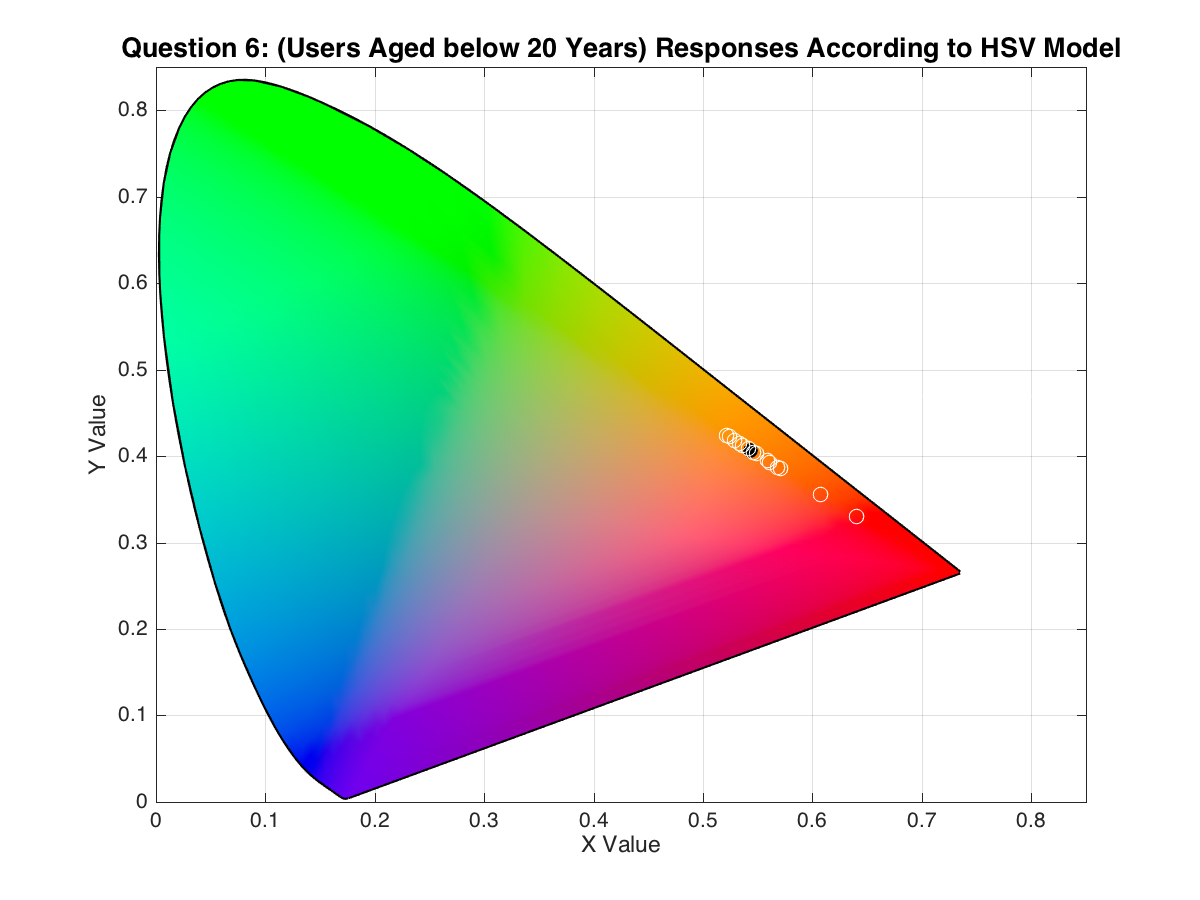
\includegraphics[width=\textwidth]{images/results/6_demo_age20_HSVresponses.png}
    \caption[Demographic Results, Question 6, Age below 20 years, according to HSV.]{Demographic Results, from Question 6, from users aged below 20 years, blended according to HSV Color Model.}
    \label{fig:age_1}
  \end{minipage}\hfill
  \begin{minipage}{0.48\textwidth}
    \centering
    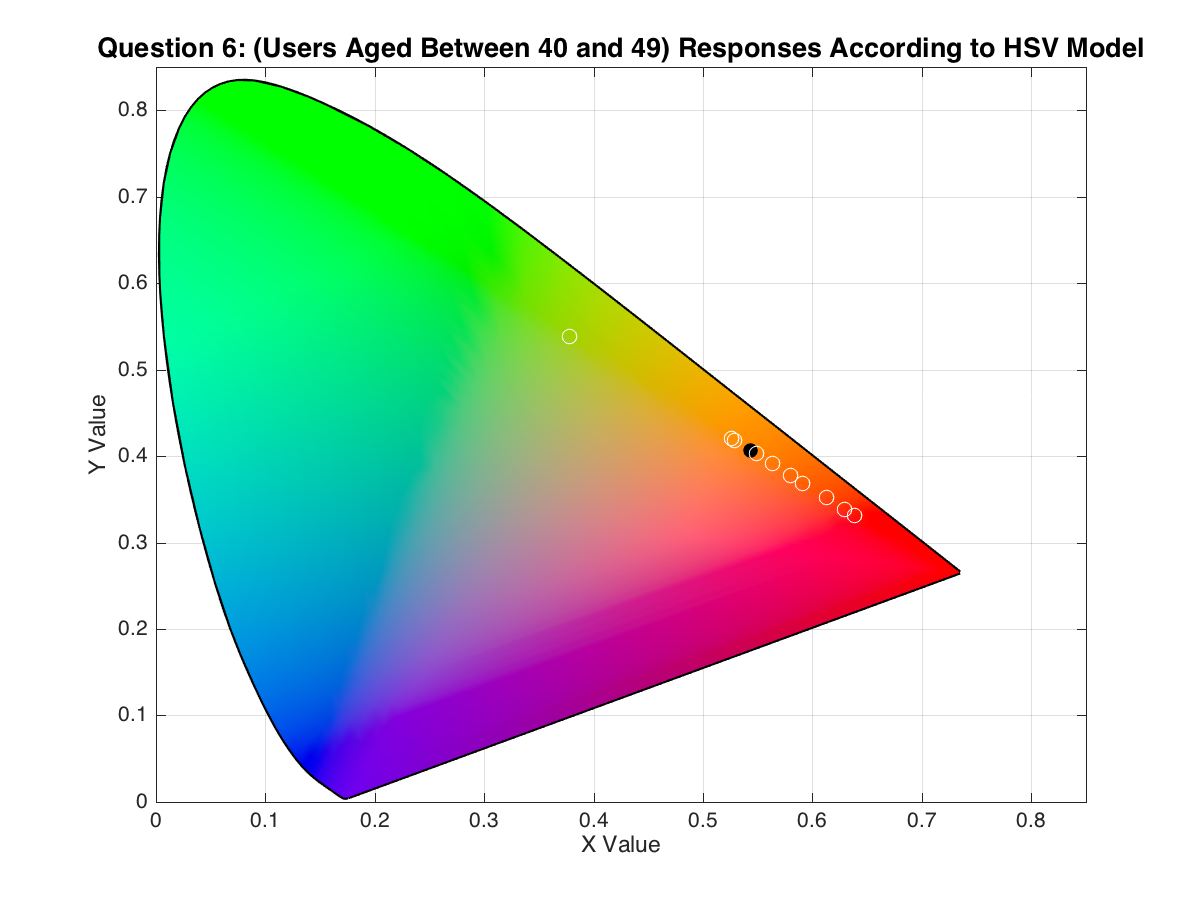
\includegraphics[width=\textwidth]{images/results/6_demo_age40_49_HSVresponses.png}
    \caption[Demographic Results, Question 6, Age between 40-49 years, according to HSV.]{Demographic Results, from Question 6, for answers given by users aged between 40 and 49 years, blended according to HSV Color Model.}
    \label{fig:age_2}
  \end{minipage}
\end{figure}
%
\subsubsection{Gender Groups}
\label{subsubsec:demo_age}
%
Recalling Table \ref{table:profiling_genderacademic}, we have collected a total of 259 users, being \ul{105 Female Users}, \ul{152 Male Users} and \ul{2 Other Gender Users}. Similarly to what was done before, we analyzed the results from
all 32 questions, for each of these gender groups, with Spearman's Correlation test: we have conclude that there are no statistically significant correlations ($\rho < 0.05$) when comparing the distances from answers blended in each color model with users' gender, for the majority of questions.
Notwithstanding, eight of them presented weak, positive and negative correlation between the gender types and the calculated distances, which have statistically significant correlation values ($\rho < 0.05$). \par
%
These questions are \ul{number six} ($r_s(6) = 0.17$, $\rho = 0.049$), \ul{nine} ($r_s(9) = -0.17$, $\rho = 0.043$), \ul{eleven} ($r_s(11) = 0.182$, $\rho = 0.038$), \ul{fifteen} ($r_s(15) = 0.22$, $\rho = 0.012$), \ul{sixteen} ($r_s(16) = -0.19, \rho = 0.024$), \ul{seventeen}
($r_s(17) = 0.18$, $\rho = 0.037$), question \ul{twenty-two} ($r_s(22) = 0.19$, $\rho = 0.024$) and, finally, question number \ul{thirty} ($r_s(30) = 0.19$, $\rho = 0.025$). \par
%
Equally to age groups' analysis, we have executed a Wilcoxon Signed-rank Test ($p < 0.05$) in order to detect significant differences which exist, between results for each color model, by gender group. The test reveals that:
%
\begin{enumerate}
  \item There are statistically significant differences ($p = 0.027$) on \ul{question nine} (expected Green-Cyan, presented a tone of Green), when blending the answers in \ul{CMYK Color Model}, between the \ul{Male} and \ul{Female} users. Among 64 cases, 38 of them presented wider distances for
  Female users, while 20 were higher for Male users;
  \item There are statistically significant differences ($p = 0.035$) on \ul{question eleven} (expected Green-Magenta, presented Orange color), when blending the answers in \ul{HSV Color Model}, between the \ul{Male} and \ul{Female} users. Among 61 cases, 23 of them presented wider distances for
  Female users, while 33 were higher for Male users;
  \item There are statistically significant differences ($p = 0.048$) on \ul{question 15} (expected Blue-Yellow, presented a tone of Green), when blending the answers in \ul{CIE-L*C*h* Color Model}, between the \ul{Male} and \ul{Female} users. Among 63 cases, 25 of them presented wider distances for
  Female users, while 33 were higher for Male users;
  \item There are statistically significant differences on \ul{question 16} (expected Blue-Yellow, presented a shade of Magenta) between the \ul{Male} and \ul{Female} users, when blending their answers according to the following color models:
  %
    \begin{itemize}
      \item \ul{RGB}, with 63 cases, 39 of them presented wider distances for Female users, while 17 were higher for Male users ($p = 0.009$);
      \item \ul{CIE-L*a*b*}, with 63 cases, 38 of them presented wider distances for Female users, while 19 were higher for Male users ($p = 0.009$);
    \end{itemize}
  %
  \item There are statistically significant differences ($p = 0.011$) on \ul{question 17} (expected Cyan-Yellow, presented Green color), when blending the answers in \ul{CIE-L*a*b* Color Model}, between the \ul{Male} and \ul{Female} users. Among 63 cases, 38 of them presented wider distances for
  Female users, while 19 were higher for Male users;
  \item There are statistically significant differences on \ul{question 23} (expected Orange, presented Red-Yellow pair), when measuring the distances from the answers according to the following Color Models:
  %
    \begin{itemize}
      \item \ul{HSV}, with 69 cases, 19 of them presented wider distances for Female users, while 38 were higher for Male users ($p = 0.005$);
      \item \ul{CMYK}, with 69 cases, 16 of them presented wider distances for Female users, while 33 were higher for Male users ($p = 0.006$);
      \item \ul{RGB}, with 69 cases, 120 of them presented wider distances for Female users, while 39 were higher for Male users ($p = 0.008$);
    \end{itemize}
  %
\end{enumerate} \par
%
These values potentiate a conclusion which was discussed in the theoretical background of this master thesis: there is a mild difference between the results from the Female gendered users, and the Male ones. It is not an absolute difference, since \textbf{not every question had presented significant
differences between gender groups}; it is \textbf{not possible to formulate a conclusion about which gender generates the wider or closer distances to the ideal answer (according to each Model)}, since there is no visible pattern about this subject. There were no significant differences between female
or male users, and the \emph{other} gendered users: this could due to the lack of a significant user sample relating the later gender. \par
%
This leads us to conclude that there is, in fact, space for a theory on \textbf{the existence of a difference in color perception by the female users, when compared with the male users}: this difference is observable in our study results, but not substantial to formulate any a formal research conclusion.
Figures \ref{fig:gender_1} and \ref{fig:gender_2} represents the statistically significant difference when blending the answers from the shade of magenta blending (question 16), in \ul{RGB Color Model}, between the Female and Male users: in these Figures, \textbf{we can distinguish an eventual lack of color
descriptive power concerning Male users} - whose answers are conveying to the grey center of the chromaticity diagram (the black dot on the Figure) - contrasting with the Female one, whose answers show a regular disposition along the edge which unites the Magenta and Red colors.
%
\begin{figure}[!htbp]
  \centering
  \begin{minipage}{0.48\textwidth}
    \centering
    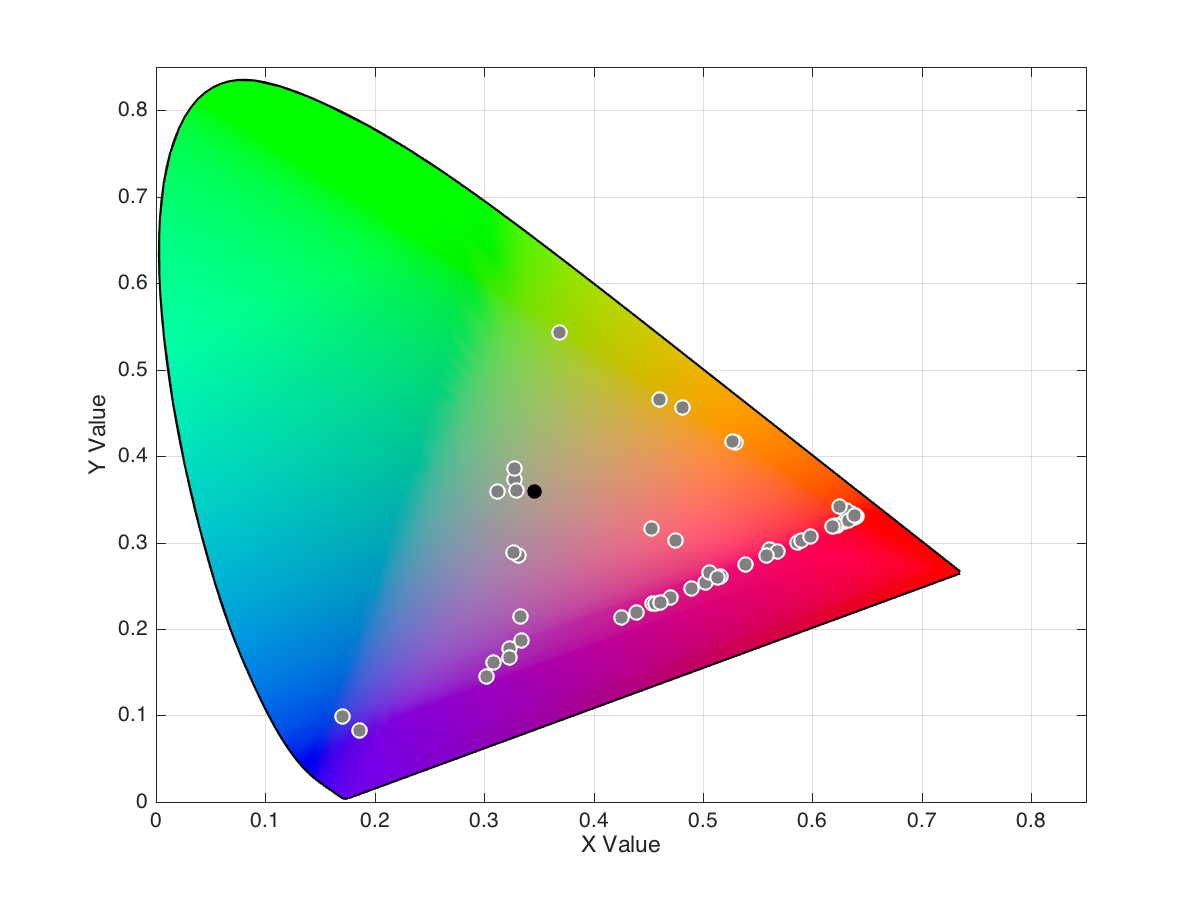
\includegraphics[width=\textwidth]{images/results/16_demo_genderF_RGBresponses.png}
    \caption[Demographic Results, Question 16, Female users, according to RGB.]{Demographic Results, from Question 16, from female users, blended according to RGB Color Model.}
    \label{fig:gender_1}
  \end{minipage}\hfill
  \begin{minipage}{0.48\textwidth}
    \centering
    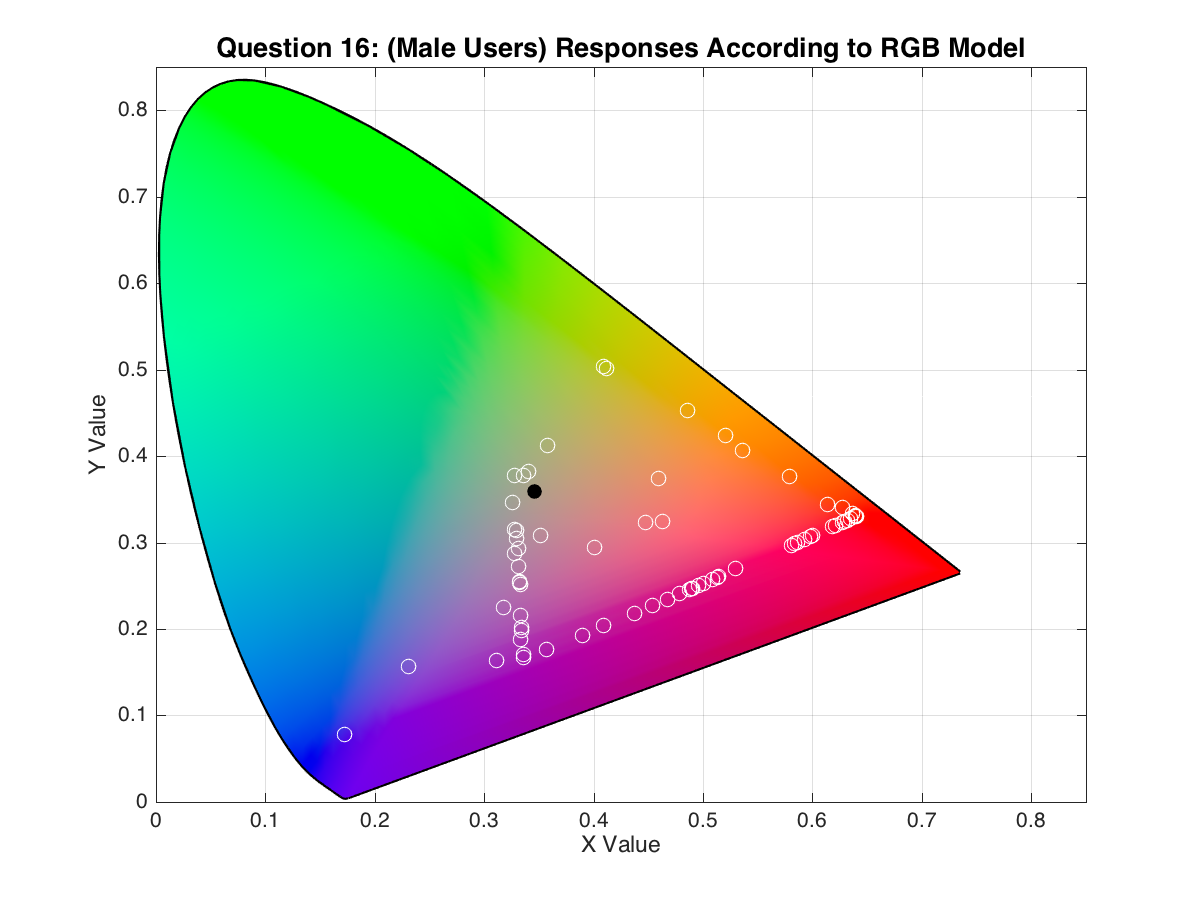
\includegraphics[width=\textwidth]{images/results/16_demo_genderM_RGBresponses.png}
    \caption[Demographic Results, Question 16, Male users, according to RGB.]{Demographic Results, from Question 16, from male users, blended according to RGB Color Model.}
    \label{fig:gender_2}
  \end{minipage}
\end{figure}
%
\subsubsection{Color Vision Deficient Users Group}
\label{subsubsec:demo_daltonic}
%
Based on the criteria defined on Section \ref{sec:impl_evaluationcriteria}, we have analyzed the collected user sample and verified if there was any user which had any type of color vision deficiency. This filtering of users was accomplished via the data collected on the \emph{Color Vision Deficiencies Test
Phase}. We had \ul{one laboratory user} which we have determined to have \textbf{\emph{Deuteranopia}, a Red-Green deficiency} and \ul{two online users} which have \textbf{\emph{Deuteranopia and Protanopia}}, each one. Since there is not enough information and data sample to perform a statistic analysis and we
did not know which colors to expect, according to each color vision deficiency when blending the answers, we performed a qualitative analysis. Though, in this Section, we give examples of some questions which presented colors that could not be correctly visualized by each color vision deficiency. \par
%
\paragraph{\ul{Magenta + Yellow = Red}}
%
In this color blending (question number eight), it was asked the users to indicate a Magenta-Yellow pair to mix into a Red color. While the non-color vision deficient users (therefore, simply called \emph{regular users}) have indicated a myriad of possible answer pairs waging between green, blue, yellow and magenta, the
color vision deficient (therefore, simply called \emph{daltonic users}) gave answer-pairs very close to the resulting color; this case can be observe on Figures \ref{fig:dalt_1} and \ref{fig:dalt_2}. This could be caused due to the fact that the Red color, for both types of deficiencies in Red-Green cones, the users
received a Yellow stimulus, instead of a Red one (recall Figure \ref{fig:correscolorblind}, of Section \ref{subsubsec:visual_deficiencies}).
%
\begin{figure}[!htbp]
  \centering
  \begin{minipage}{0.48\textwidth}
    \centering
    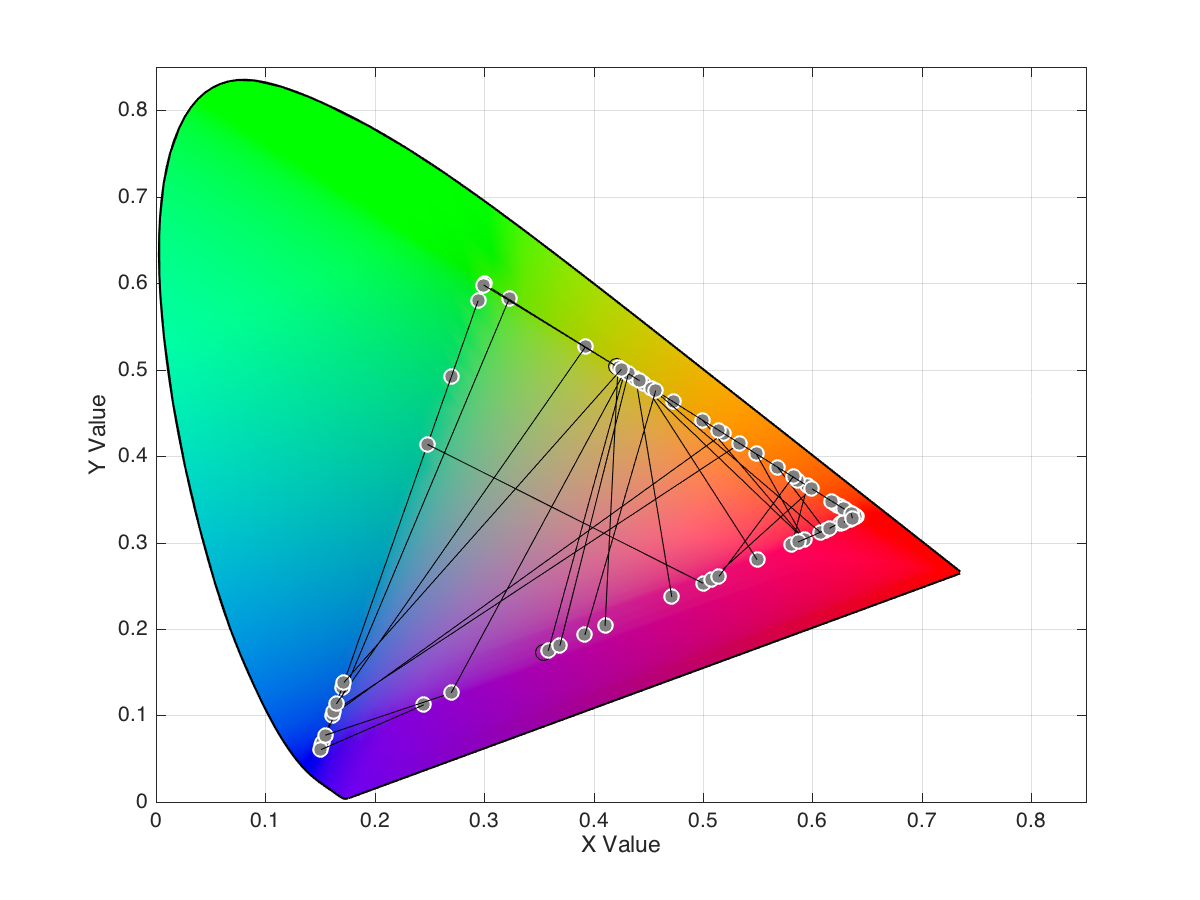
\includegraphics[width=\textwidth]{images/results/8_online_regularUsers.png}
    \caption[Online: Answers for Question 8, from regular users.]{Online: Answers for Question 8, from regular users.}
    \label{fig:dalt_1}
  \end{minipage}\hfill
  \begin{minipage}{0.48\textwidth}
    \centering
    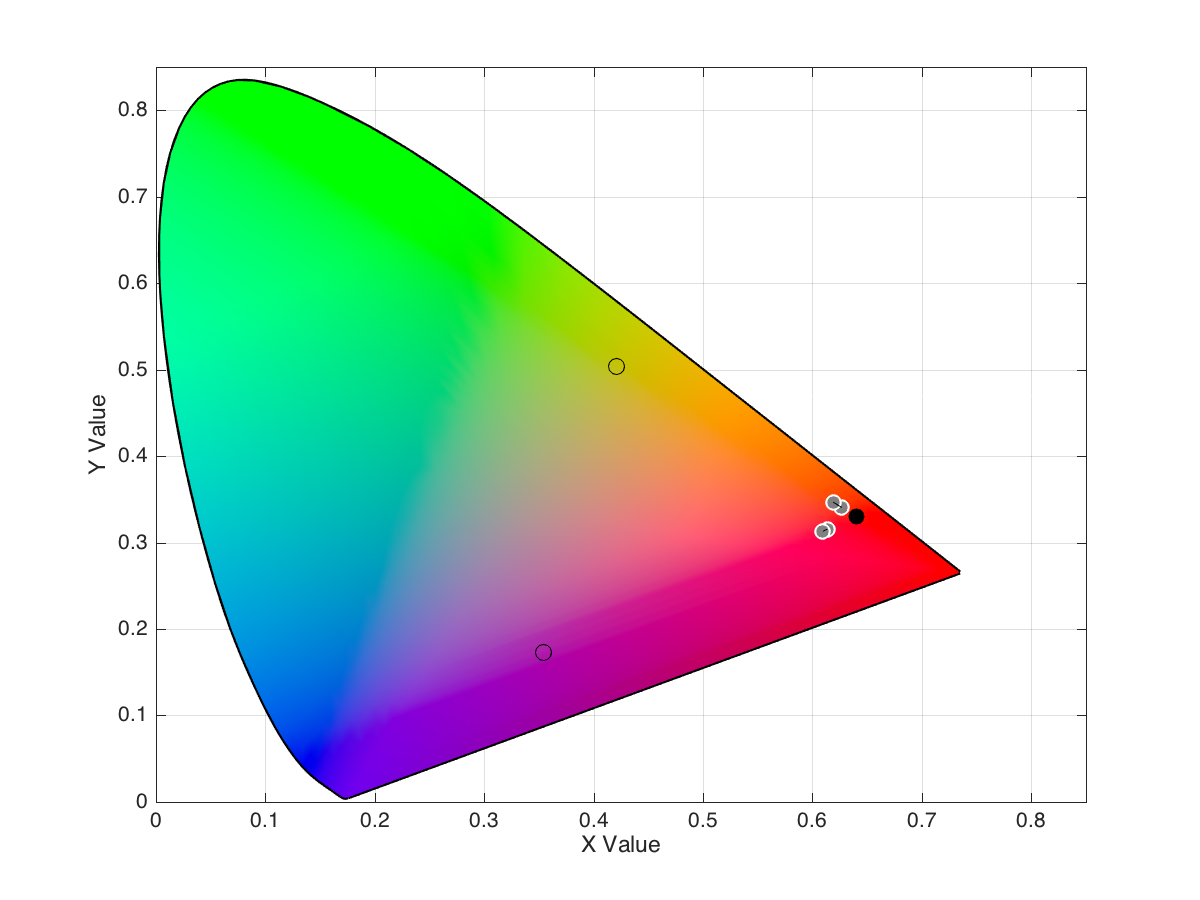
\includegraphics[width=\textwidth]{images/results/8_online_daltonicUsers.png}
    \caption[Online: Answers for Question 8, from daltonic users.]{Online: Answers for Question 8, from daltonic users.}
    \label{fig:dalt_2}
  \end{minipage}
\end{figure} \par
%
\paragraph{\ul{Cyan + Yellow = Green}}
%
On the other hand, when we presented one of the blending which collected the best results from all (question 17), the users answered in a similar fashion from the regular users. It was asked the users to indicate a Cyan-Yellow pair to mix into a Green color, and the three daltonic users from both study environment have
answered with similar answer-pairs. The laboratory user answered with a Green-Green pair, while the online users answered with a Yellow-Cyan one; this could have many reasons to happen, since these color vision deficiencies transform the Green presented color onto a Yellow shade, but preserves the Blue color as it is, and
the yellow color is a very common color to perceive among these deficiencies. \par
%
We could make the following analysis: the laboratory user either mixed Yellow-Yellow (adjusted to its color vision deficiency) because he didn't realize the blending-basis, or simply because for him, the yellow color cannot be decomposed onto two primitive colors; respecting the online users, they could have provided this
pair since they know for fact to which regular color the color they see correspond to, or because they see a darker shade of yellow (presented) and wanted to indicate a blending basis of Yellow and a darker color like Blue, to darken the mixture. Figures \ref{fig:dalt_3} and \ref{fig:dalt_4} help us supporting this explanation.
%
\begin{figure}[!htbp]
  \centering
  \begin{minipage}{0.48\textwidth}
    \centering
    \includegraphics[width=\textwidth]{images/results/17_lab_daltonicUsers.png}
    \caption[Laboratory: Answers for Question 17, from daltonic users.]{Laboratory: Answers for Question 17, from daltonic users.}
    \label{fig:dalt_3}
  \end{minipage}\hfill
  \begin{minipage}{0.48\textwidth}
    \centering
    \includegraphics[width=\textwidth]{images/results/17_online_daltonicUsers.png}
    \caption[Online: Answers for Question 17, from daltonic users.]{Online: Answers for Question 17, from daltonic users.}
    \label{fig:dalt_4}
  \end{minipage}
\end{figure} \\ \par
%
This is a \textbf{purely informal analysis}, since it does not provide any type of statistics and does not produce any type of research conclusion: in order to obtain factual conclusions about this investigation subject, it should be developed an entire user study with daltonic users, providing the necessary amount of data to be correctly
analyzed.
%
%%%%%%%%%%%%%%%%%%%%%%%%%%%%%%%%%%%%%%%%%%%%%%%%%%%%%%%%%%%%%%%%%%%%%%%%%%%%%%%%%%%%%%%%%%%%%%%%%%%%%%%%%%%%%%%%%%%%%%%%%%%%%%%%%%%%%%%%%%%%%%%%%%%
%                                                                DISCUSSION                                                                       %
%%%%%%%%%%%%%%%%%%%%%%%%%%%%%%%%%%%%%%%%%%%%%%%%%%%%%%%%%%%%%%%%%%%%%%%%%%%%%%%%%%%%%%%%%%%%%%%%%%%%%%%%%%%%%%%%%%%%%%%%%%%%%%%%%%%%%%%%%%%%%%%%%%%
%
\section{Discussion}
\label{sec:results_discussion}
%
The goal of this color study was to: \textbf{study a way to present color information which does not influence color perception}, \textbf{understand if there is any mental organization of color} and \textbf{study the influence of discrete and continuous color scales} on
user's answers. Additionally, it was relevant to understand which color model stood as the best to blend colors which are more similar to users' expectation. This user study was developed in two different conditions: in a \textbf{Laboratory Environment}, which allowed us
to calibrate ans control the entire study conditions, and in a \textbf{Online Environment}, which allowed us to broadcast our study to a larger set of users. \par
%
We have defined a set of questions which we wanted to answer to, as follows:
\textbf{Q1:} Which Color Model meets best the users' expectations, when blending two colors?,
\textbf{Q2:} Is there evidence of a spatial arrangement of colors, when users are indicating possible color mixtures' results?, and
\textbf{Q3:} Are there evidences from differences across demographic groups, such as the age or gender?.
%
We have performed a statistical analysis of the processed data obtained from the user study: the main data which was analyzed was the one obtained in the laboratory environment, being the online data only the corroboration of the main data. We have started by drafting a
profile from the users which we have obtained the data from: our user sample is composed by \textbf{259 users}, being 105 Females, 152 Males and a minority of 2 Other gendered users, \textbf{171 of these} have a High-Degree of Education and \textbf{215 users} have
Portuguese Nationality. \par
%
In order to study which color model yields the best results, we have interpolated each answer-pair given by the users according to each color model in study: HSV, CIE-L*C*h*, CMYK, RGB and CIE-L*a*b*. These interpolations were performed on the subset of questions comprised between
number 1 and 17, which represent the questions in which the result of a given mixture was given, and the user had to answer the question by indicating the answer-pair which he thought it would fit the ideal blending-basis.
We have observed that \textbf{the color blending which constantly yielded the best results across all color models is the mixing of Red-Yellow, to achieve Orange}, while the mixture which provided the worst results when evaluating the distance from the user's
answers and the ideal answers, is \textbf{the blending of Green-Magenta, resulting in a Blue shade}: these results are consistent with the ones collected by Gama and Gonçalves \cite{Gama20141} before, which concluded that the success rates were higher for blending pairs
like Red-Yellow, and worst for pairs which correspond to a wider angle in a Hue circle. For instance, \textbf{blending Cyan and Yellow, to obtain Green} had very good results, generating the lowest values for evaluated descriptive statistics across each
every color model ($\overline{x}$, $s$, $s^2$). These results are, also, \textbf{consistent with the fact that the human color perception is conditioned by the amount of Cones present in our eyes} since the users have more descriptive power for colors near the
green zone of the spectrum, due to the fact that the eye has substantially more green sensitive cones than blue ones, indicating that minimum variations within Blue colors could not be detected. \par
%
When analyzing the answers by Color Model, we can observe that \textbf{the HSV Color Model, along with CMYK and RGB, is the one which presents the lowest standard deviation of distances} between the results from the online environment, while \textbf{the Color Model
which presented the lowest mean value for distances was the CMYK Color Model}. The RGB, HSV and CIE-L*a*b* Color Models all generate values very similar to each other, so \textbf{further studies should focus on discerning which color model is better than others, between
HSV, RGB and CIE-L*a*b*}, since there were no relevant differences among them. \par
%
On the other hand, the CIE-L*C*h* Color Model is the one which typically provided the worst results across all color blendings, therefore being \textbf{the one which least resembles the users' expectations when blending colors}. The CMYK Color Model is, by far, the one
which presents the best results for most of the descriptive statistics, being corroborated by the results from the online environment: the distances from the given answers when blended according to the CMYK Color Model, presented consistently the lowest values across
all questions. In fact, the questions which yielded better results are majorly related to primitives of the CMYK color model; this success could be related to the fact that people tend to formulate mental models of color based on ink mixing in childhood
\cite{Gossett2004}, mostly associating it to Red, Yellow, Blue (RYB) and CMYK Color Models without even knowing it: \textbf{These results indicate that CMYK is a highly compatible color model with the users expectations}. For these reasons, we can answer question
\textbf{Q1}, stating that \textbf{the color model which most resembles the user's expectation, when blending two colors according to a given result, is the CMYK Color Model}. Since CMYK is an additive color model, it is safe to say that \ul{the type of color models which
most resembles the user's expectation, when blending two colors according to a given result, is a subtractive color model}. \par
%
It is also interesting to observe that the users are able to blend primary colors (Red, Green, Blue, Cyan, Magenta and Yellow) using other primary colors as the blending-basis: however, the results obtained for \textbf{Blue and Cyan are consistent with the ones
obtained previously}: there is no strong evidence that the users can produce Blue (or blue-derived) color blendings. In opposition, when \textbf{creating Green, Magenta and Yellow}, the users revealed some basic conception of blending their basis, with more emphasis
on the process of creating Magenta: users have indicated more detailed shades of Red to create the color mixture, contrary to other color blends evaluated, which may have implications on the level of detail that the displaying of color should have. This leads us to
answer question \textbf{Q2}: \textbf{for color blendings which involve the Red color there is, in fact, evidence that the users sort the colors when indicating the blending-basis, revealing some mental color organization}: in the latter case of the Magenta blending, users may have indicated
first the Red shades, since it is a color that is more similar to Magenta (the resulting one) and users may have used it to start the mixture, just like when using paint colors. \par
%
Besides asking our users to indicate us the two primitives which composed a color blending of two colors, we intended to go further: comprehend if more than detecting two colors of a mixture, a user is capable of mentally blend two given colors and indicate us its results.
Therefore, we reverted the way blendings were presented, giving the two primitives of the blending to the user, offering at the same time a color slider which contained discretized pre-calculated values (which were nothing more than all the results of all questions,
blended accordingly to all color models). The distances for these questions were higher than the previous ones: this could be due to the fact \textbf{we have only presented discretized colors as options, and did not leave any wiggle-room for the user to indicate other
colors which he thought it could be more appropriate}. For certain colors (\emph{e.g.} the orange blending) the results were equally good, since there are \textbf{color blendings which users are more familiar with and, therefore, are more intuitive}. \par
%
We have also performed a demographic analysis to ascertain if there was any plausible difference present in our dataset, between demographic groups. We have conducted an analysis \emph{per} age groups (users aged below 20 years, between 20-29, 30-39, 40-49, 50-59 and
above 60 years) and gender groups (Female, Male and Other gendered). Regarding the \ul{age groups}, we have not found relevant differences between age groups, since not every color blending had presented statistically significant differences between the groups; however,
from the ones which had presented differences, the users aged between 40 and 49 years were present in every difference detected. Still, \textbf{we do not have enough ground truth to support a conclusion about the existence of age differences}. \par
%
We cannot say the same thing about \ul{gender groups} differences: there is a mild difference between the results from the Female gendered users, and the Male ones. It is not an absolute difference, since not every question had presented significant differences between
gender groups; also, it is not possible to formulate a conclusion about which gender generates the wider or closer distances to the ideal answer (according to each Model), since there is no visible pattern about this subject. There were no significant differences
between female or male users, and the other gendered users: this could due to the lack of a significant user sample relating the later gender. This leads us to conclude that \textbf{there is, in fact, space for a theory on the existence of a difference in color
perception by the female users, when compared with the male users}: this difference is observable in our study results, but not substantial to formulate any a formal research conclusion. \par
%
Finally, we have studied the users' effort in blending colors: the results are in agreement with the ones collected and concluded before, in which the blending of Red-Green resulting in Yellow, blending of Red-Yellow and Green-Magenta, both resulting in Orange and the
blending of Cyan-Yellow resulting in Green were the mixtures which, according to the users’ answers, had the lowest effort when blending, consequently the highest rating of easiness. It is interesting to observe that the results for the generality of questions encircle
the rating of two and three, on a scale from one to five, which could indicate that apart from the obvious color blendings which proved to yield the best results, all \textbf{the other blendings show nor an easy or hard level of effort to mix the basis}. Answering question
\textbf{Q3}, \textbf{it is possible to observe that there are evidences of difference between demographic groups, but only between genders}.
%
\subsection{Guidelines for the usage of Color Blending}
\label{subsec:guidelines}
%
The following list enumerates a set of guidelines which we are able to formulate, based on our user study, about the usage of color blending when sketching visualizations:
%
\begin{enumerate}
  \item To maximize the compatibility with the user's expectations, \textbf{choose} color blends which present Orange shades based on mixing Red and Yellow.
  \item Color blends which present a resulting color of Green are welcomed by the user, since it is easier for him to detect smaller changes on \textbf{green shades}, than on blue shades.
  \item The Yellow color provides very good results, when blending Red and Yellow. The CMYK Color Model is the one which has the best results, according to user's expectations.
  \item To maximize the compatibility with the user's expectations, \textbf{avoid} presenting colors which are near Blue shades, since the user's perception does not yield the best results.
  \item When using Red shades, the best blending-basis is Red and Magenta. If the resulting color is presented instead of the basis, the color model which is has better results is the CMYK; however,
  if the blending-basis is presented and the result asked, avoid the CMYK and present the result interpolated according to HSV Color Model.
  \item Presenting the resultant color from a given blending, generally, produces better results than asking the user to blend the color according to his mental model of color.
  \item The color model which best resembles the user's expectation is a subtractive one, for example \textbf{CMYK}. However, do \textbf{not} use it to present Blue shades since it yields higher distances to user's expectation.
  \item If the usage of CMYK Color Model is not convenient, the usage of HSV, RGB and CIE-L*a*b* produces similar results between each other, but slightly weaker results when compared to CMYK.
  \item Avoid using the CIE-L*C*h* Color Model when blending colors according to the user's expectations. Except when asking the result for the following color blendings: Green and Cyan, Blue and Cyan, Blue and Magenta, and
  Red and Yellow.
  \item Consider including the white color in the set of presented colors for the user to work with.
\end{enumerate}
%
\subsection{Calibration Resiliency}
\label{subsec:results_calibration}
%
During the analysis of the dataset, we verified that there was a smaller set of five online users which had presented erratic calibration
values. Since these users could provide interesting values to establish a comparison between values gathered on a calibrated,
\emph{versus} an uncalibrated study environment, we have kept them in a separate dataset for comparisons. These users, similarly to color
vision deficient users, were subject of a qualitative comparison, due to the fact that there is insufficient data to demonstrate significant
comparisons. \par
%
Since the laboratory users performed the color study inside a controlled and calibrated environment, they are not examined in this analysis.
Performing a Friedman Test over the results from calibrated users and uncalibrated users, we concluded that only two questions
show statistically significant differences between results: they are question two ($\chi^2 = 24.853$, $p < 0.05$) an question 13
($\chi^2 = 17.209$, $p < 0.05$). However, when analyzing the chromaticity diagrams from question two, present in Figures \ref{fig:uncal_1}
and \ref{fig:uncal_2}, we end up concluding that \textbf{there is no substantial difference between calibrated and uncalibrated results}.
Remember that question 2 asked for a answer-pair of Red-Blue to a Magenta color presented.
%
\begin{figure}[!htbp]
  \centering
  \begin{minipage}{0.48\textwidth}
    \centering
    \includegraphics[width=\textwidth]{images/results/2_online_regularUsers.png}
    \caption[Online: Answers for Question 2, from calibrated users.]{Online: Answers for Question 2, from calibrated users.}
    \label{fig:uncal_1}
  \end{minipage}\hfill
  \begin{minipage}{0.48\textwidth}
    \centering
    \includegraphics[width=\textwidth]{images/results/2_online_uncalibratedUsers.png}
    \caption[Online: Answers for Question 2, from uncalibrated users.]{Online: Answers for Question 2, from uncalibrated users.}
    \label{fig:uncal_2}
  \end{minipage}
\end{figure} \par
%
To consider that a user presented a calibration which was not correct, we based our evaluation on the \textbf{Calibration Test Phase} of the
study: there is still the chance that, despite the user provided wrong values considering the ones expected, his calibration was in fact
correct to carry out the study. Since the majority of questions of this user study revealed no significant difference between calibrations,
we can state that \textbf{this color study was resilient to changes in calibration values}; however, there is \textbf{no relevant research
conclusions to elaborate from this subject}.
%
\subsection{Implications for InfoVis}
\label{subsec:results_discussion_infovis}
%
This research produced a set of useful results which could have some impact in the \gls{InfoVis} Research area. As it is know,
conveying data values through marks and channels is typical of an infovis: via geometric shapes, their size, length, motion, or hue;
particularly, the latter is an interesting topic, which is to convey information via color. Using one color to transmit the information
contained in one variable is straightforward (though discussion may be raised about which is the best color), the not-so-trivial subject about
this is when we want to carry more than one variable with different colors: do color blendings effectively work when two colors are mixed and
presented to the user? \par
%
There are many ways to tackle the blending of colors when presenting two data variables in an infovis: for example, one can attribute a color
in its maximum saturation to each variable and simply blend them, presenting to the user the result already digested. However, this raises
many questions such as \emph{Which color model should be used to present the color blending result?}, or \emph{Which color blending should be
used to provide the best results, as well as creating an appealing visualization?}; one can also ask if \emph{Is there any rule-of-thumb for
adding relative quantities of each color?}. \par
%
Though this subject may be extended to blendings with more than two colors, we believed that \textbf{the more colors involved in a color mixture,
the greater the confusion which may happen when trying to interpret the results carried in each color}: this could occur, since the majority of
users may not be familiar with the process of mixing colors, as it is not a task conducted out recurrently in a daily basis. If the user is not
familiar with the process, this could cause an overhead when he tries to interpret the visualization and, if he cannot interpret it, whatever
happens next may lead him to leave the visualization since he may not be able to overcome the inherent learning curve. \par
%
It is important to understand what is best to keep the user's focus, while corresponding to his expectations at the same time: is it to present the
information visualization already with the colors blended, leaving to the user the task of perceiving the underlying values? Or is it better to give
the user the freedom to blend the colors which he feels more comfortable with? We conducted a color study with a sample of users, where we presented
a set of colors which resulted from blending pairs of two colors according to five color models (HSV, CMYK, RGB, CIE-L*a*b* and CIE-L*C*h*). The colors
were presented in the study interface in agreement with the HSV Color Model, since it was the one which could provide the \emph{tools} of presenting the
color as we wanted in the visualization: varying \textbf{H}ue, maximum \textbf{S}aturation and maximum \textbf{V}alue, so we could range the colors we
wanted to present inside the range of $[0º ; 360º]$. It is totally valid to use the HSV Color Model to manipulate the colors presented in a information
visualization (typically developed using web technologies), since it provides light colors, shades and greys only by varying the H, S and V primitives. \par
%
Though, we have found that \textbf{the color model which better corresponds to the user's blending expectation is the CMYK Color Model}: this is
notably interesting, since we can relate this result with the known fact that the users created their mental models of color according to infant
experiences of paint pigments blending. In fact, the users are much more familiar with blending paint colors, than blending light colors: except
for the users which are familiar with RGB Color Model (typically the Computer Science ones), the majority of users formulated their mental model of
color in accordance with subtractive color models. \par
%
CMYK, then, proves to be the color model which most likely the users would follow if they had to decompose a color presented. There are some artifacts
which could support the color blending analysis, like Legends, but it would be better for the user if the information visualization is self-contained
and he did not depend on analyzing other artifacts. This is what a visualization Designer, ultimately, wants: to create mappings which are natural
for the user to follow and compose. We have discovered that the \textbf{color blendings which are more inherent to the user are the ones which
generate Green, Orange or Yellow}, being \textbf{Blue derived shades the least detectable color blendings}: again, this is consistent with the known
fact that the human perception of color is deeply affected by the number of color-detecting cells in the eye, which have higher frequencies for
\textbf{M}edium and \textbf{L}arge Wavelength Sensitive Cones (Green-Red color perception), than \textbf{S}mall Wavelength Sensitive Cones
(Blue color perception). \par
%
The creation of any visualization should be supported by a convenient color scale, which should be adapted to the type of data which is trying to
convey: if the data we are conveying does need an ordering, then \ul{no Hue} should be provided since the users will see categories that are not there.
On the other hand, it should not be provided \ul{any Luminance or Saturation} when categories are wanted, because the users will see order that are not
there. In our study, we provided a continuous color scale when we asked for the color-pair which originated a given result color, since the underlying
values of the slider were simply the Hue angles from the HSV color model; contrary, we have presented a discrete color scale when asked for the result
of blending a given blending-basis, since the values of the slider were the pre-calculated results according to each color model. Our user study confirms
that \textbf{the usage of continuous color scales should be limited to cases in which the user is intended to oscillate the value of a variable and adjust
it as he may}, and that \textbf{the usage of discrete color scales should be indicated when giving the user tools to blend colors associated to
pre-defined containers of information} as Gama and Gonçalves stated \cite{Gama20142}.\par
%
We have gathered a generous amount of data from users which provide only one answer, followed by a white color; these users lead us to conclude that
\textbf{it would be of major interest to the user to include the white color in a color scale} so he can adjust the percentage of color which he wants
to indicate. This would be interesting when providing visualizations in which the user could perceive a relative amount of data associated with a color,
for example in a choropleth (\emph{e.g.} Figure \ref{fig:choropleth}), where the user is presented with the same color but in different shades or tones. \par
%
It was also interesting to observe that the users are capable of formulating better the blending-basis when given the result, than formulating the result
when given the blending-basis; this could be related to act of creating and imagining the colors which are not given, it may be easier for the user to
indicate colors which he knows (which belong to a set of \emph{named-colors}, like Red, Green or Yellow), than to create a product of two colors. For
example, \textbf{it was easier for the users to indicate that \ul{Magenta and Yellow result in a Red shade} when given the result, than when the basis
was given}. Imagining an information visualization, it is the same as stating that \textbf{it is best for the user to perceive an already blended color
and process it according to its mental model of color}, than to give a white screen and ask the user to create the color blendings. \par
%
Additionally, it would be interesting to explore the differences between genders (Female and Male) and adapt the amount of \emph{descriptiveness} visually
perceived by the user according to its gender; since it is plausible that there is, in fact, some mild difference between the color descriptive power of
man and woman, \textbf{an information visualization that could provide such feature would be, besides more enjoyable, more adapted to the descriptive
capabilities of each user} and capable of providing better results and less frustration.
%
